\documentclass[aspectratio=169,12pt]{beamer}
\usepackage[utf8]{inputenc}
\usepackage[T5]{fontenc}
\usepackage[vietnamese]{babel}
\usepackage{lmodern}
\usepackage{graphicx}
\usepackage{booktabs}
\usepackage{tabularx}
\usepackage{multicol}
\usepackage{tikz}
\usepackage{xcolor}

\usetheme{Madrid}
\usefonttheme{professionalfonts}

% --- Custom Colors & Settings ---
\definecolor{UBrandBlue}{RGB}{0, 71, 155}
\definecolor{UBrandGold}{RGB}{255, 184, 28}
\setbeamercolor{palette primary}{bg=UBrandBlue,fg=white}
\setbeamercolor{palette secondary}{bg=UBrandGold,fg=black}
\setbeamercolor{palette tertiary}{bg=UBrandBlue!80!black,fg=white}
\setbeamercolor{title}{bg=UBrandBlue,fg=white}
\setbeamercolor{item}{fg=UBrandBlue}


\title[Thực hành - Chương 09]{CHƯƠNG 9}
\subtitle{Trình bày Kết quả Phân tích Dữ liệu}
\author[Giảng viên]{Trí tuệ Nhân tạo cho Kế toán (AI in Accounting)}
\institute[Đại học]{Khoa Kế toán - Kiểm toán}
\date{Bài giảng Thực hành 09}

\begin{document}

\begin{frame}
    \titlepage
\end{frame}

\begin{frame}{Intro 9.0}

    \begin{figure}[h]
        \centering
        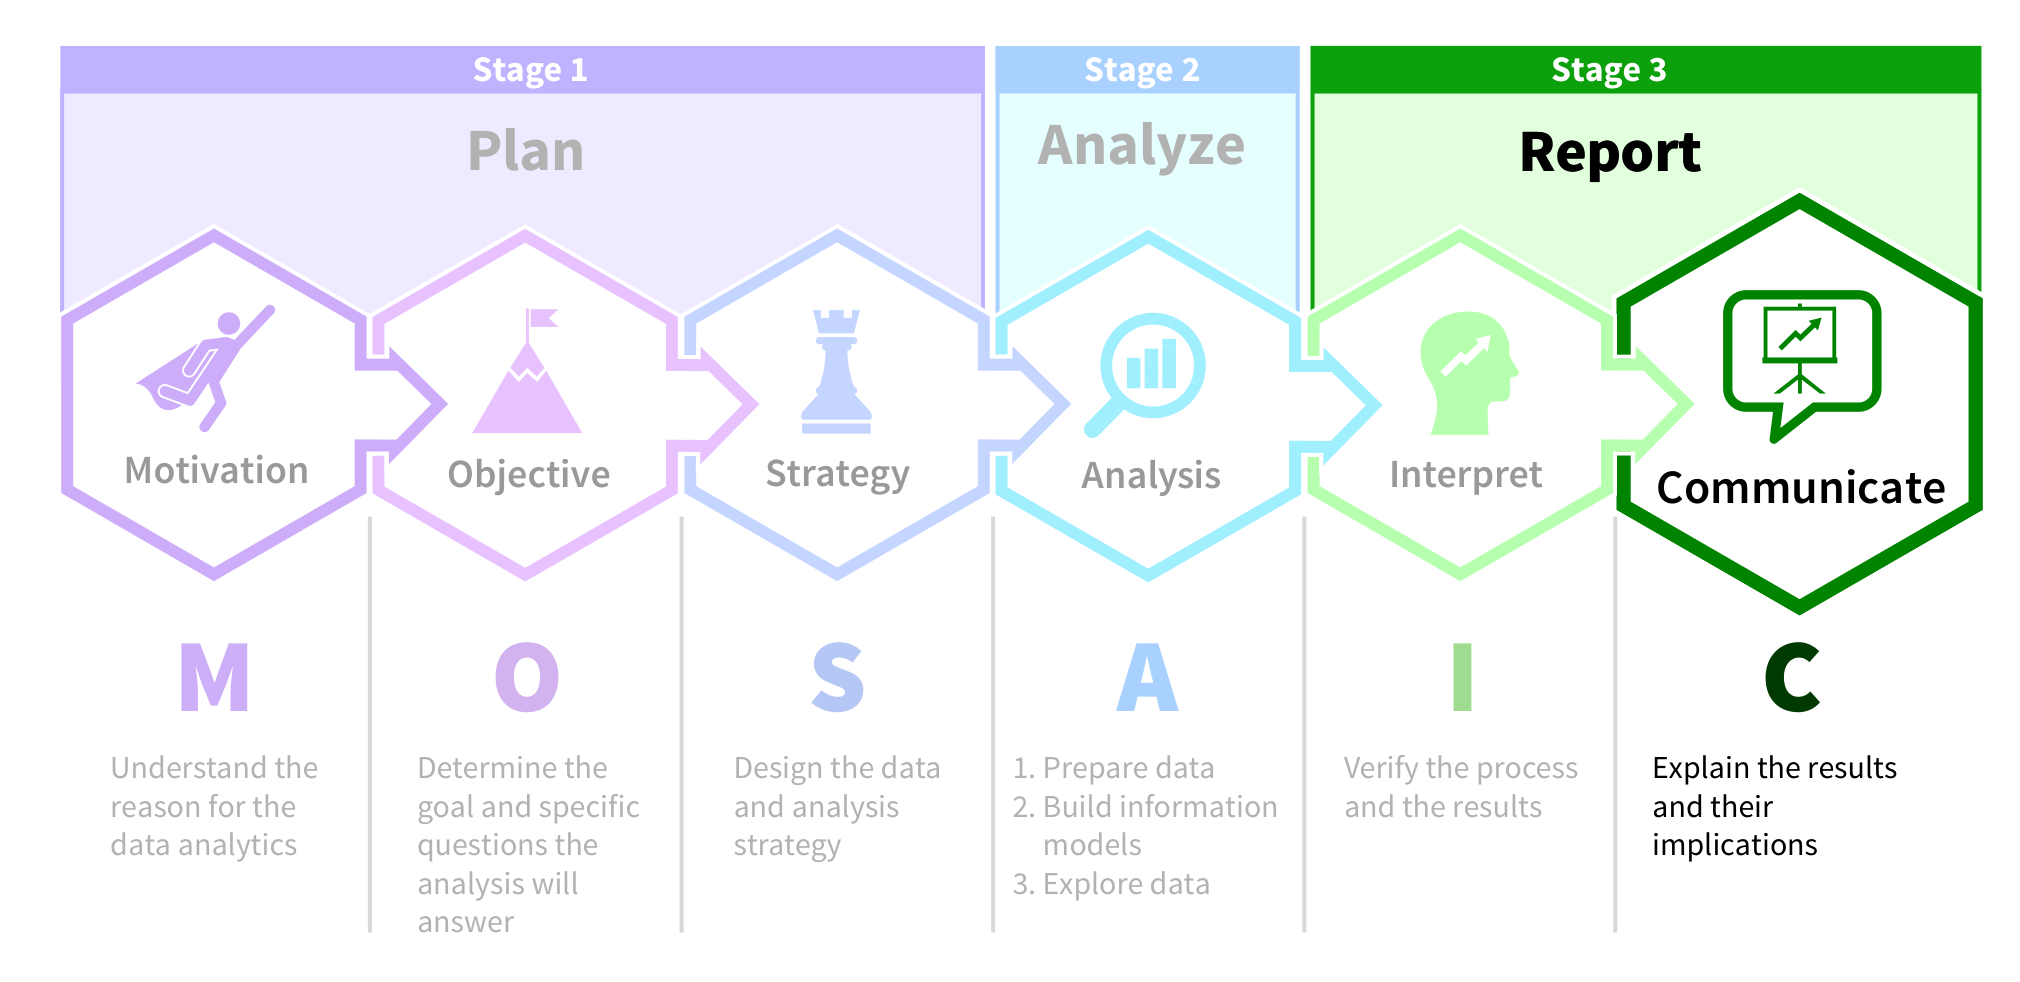
\includegraphics[width=0.95\textwidth,height=0.75\textheight,keepaspectratio]{../textbookForPractice/Figures/Ch_09/Intro 9.0.png}
    \end{figure}
\end{frame}

\begin{frame}{ILLUSTRATION 9.1}

    \begin{figure}[h]
        \centering
        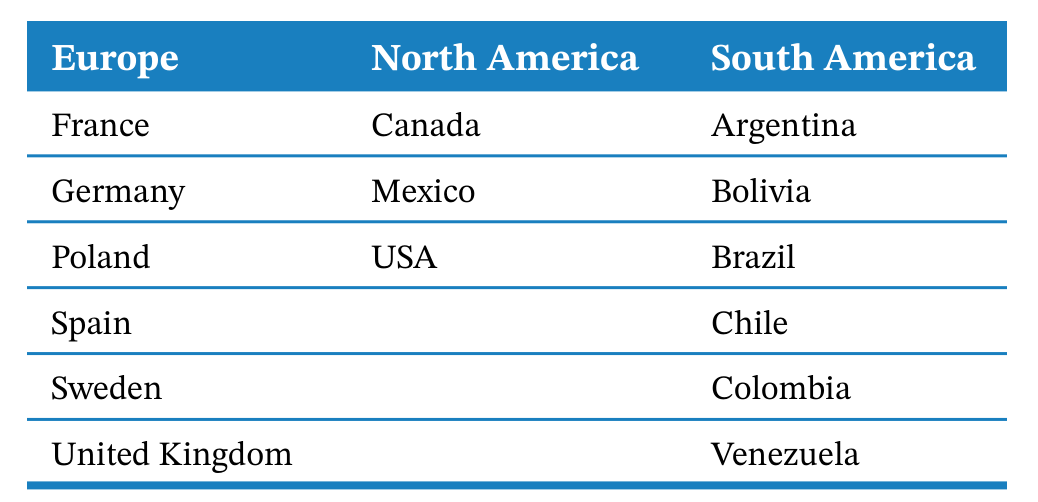
\includegraphics[width=0.95\textwidth,height=0.75\textheight,keepaspectratio]{../textbookForPractice/Figures/Ch_09/ILLUSTRATION 9.1.png}
    \end{figure}
\end{frame}

\begin{frame}{ILLUSTRATION 9.2}

    \begin{figure}[h]
        \centering
        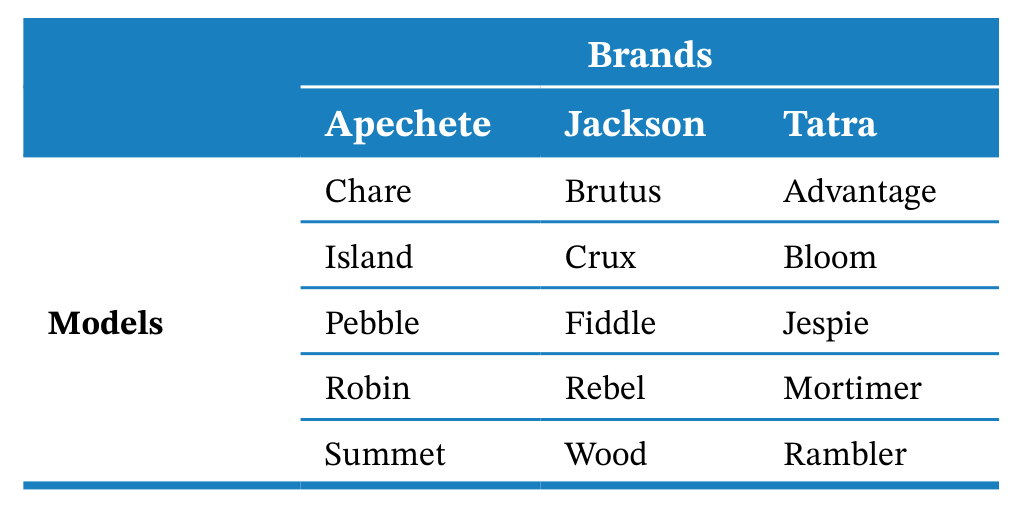
\includegraphics[width=0.95\textwidth,height=0.75\textheight,keepaspectratio]{../textbookForPractice/Figures/Ch_09/ILLUSTRATION 9.2.png}
    \end{figure}
\end{frame}

\begin{frame}{ILLUSTRATION 9.3}

    \begin{figure}[h]
        \centering
        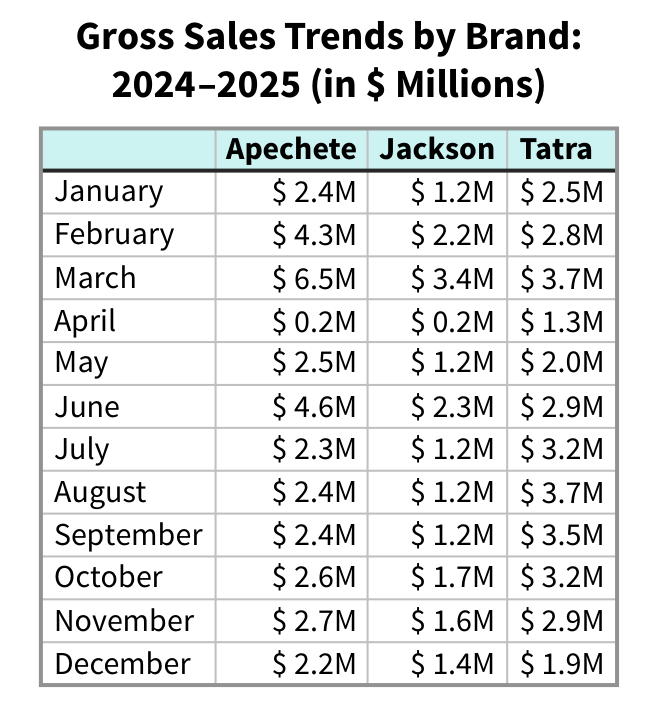
\includegraphics[width=0.95\textwidth,height=0.75\textheight,keepaspectratio]{../textbookForPractice/Figures/Ch_09/ILLUSTRATION 9.3.png}
    \end{figure}
\end{frame}

\begin{frame}{Chương 9: Trình bày Kết quả Phân tích Dữ liệu}
\begin{itemize}
    \item \textbf{Mục tiêu:} Xây dựng năng lực phân tích dữ liệu và trình bày kết quả cho kế toán viên.
    \item \textbf{Tầm quan trọng:} Đóng vai trò là cầu nối giữa dữ liệu kỹ thuật và quyết định chiến lược.
    \item \textbf{Lộ trình:} Từ định nghĩa câu chuyện dữ liệu đến tạo trực quan hóa và nhận diện các biểu đồ gây hiểu lầm.
\end{itemize}
\end{frame}

\begin{frame}{ILLUSTRATION 9.4}

    \begin{figure}[h]
        \centering
        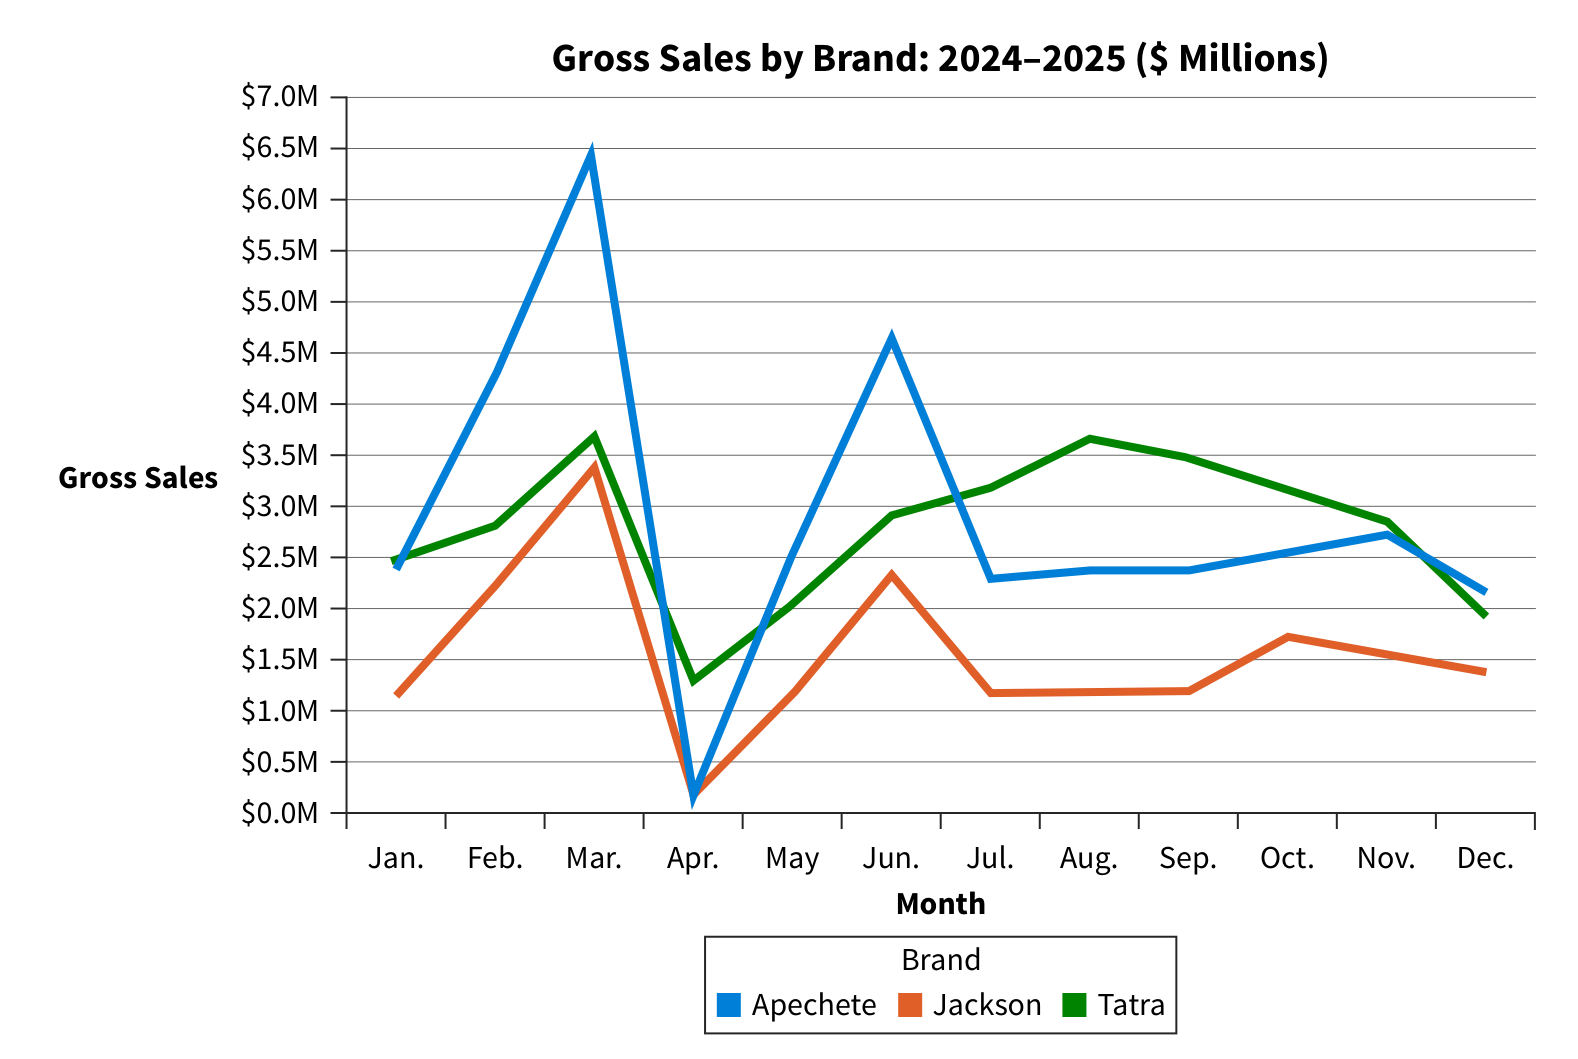
\includegraphics[width=0.95\textwidth,height=0.75\textheight,keepaspectratio]{../textbookForPractice/Figures/Ch_09/ILLUSTRATION 9.4.png}
    \end{figure}
\end{frame}

\begin{frame}{ILLUSTRATION 9.5}

    \begin{figure}[h]
        \centering
        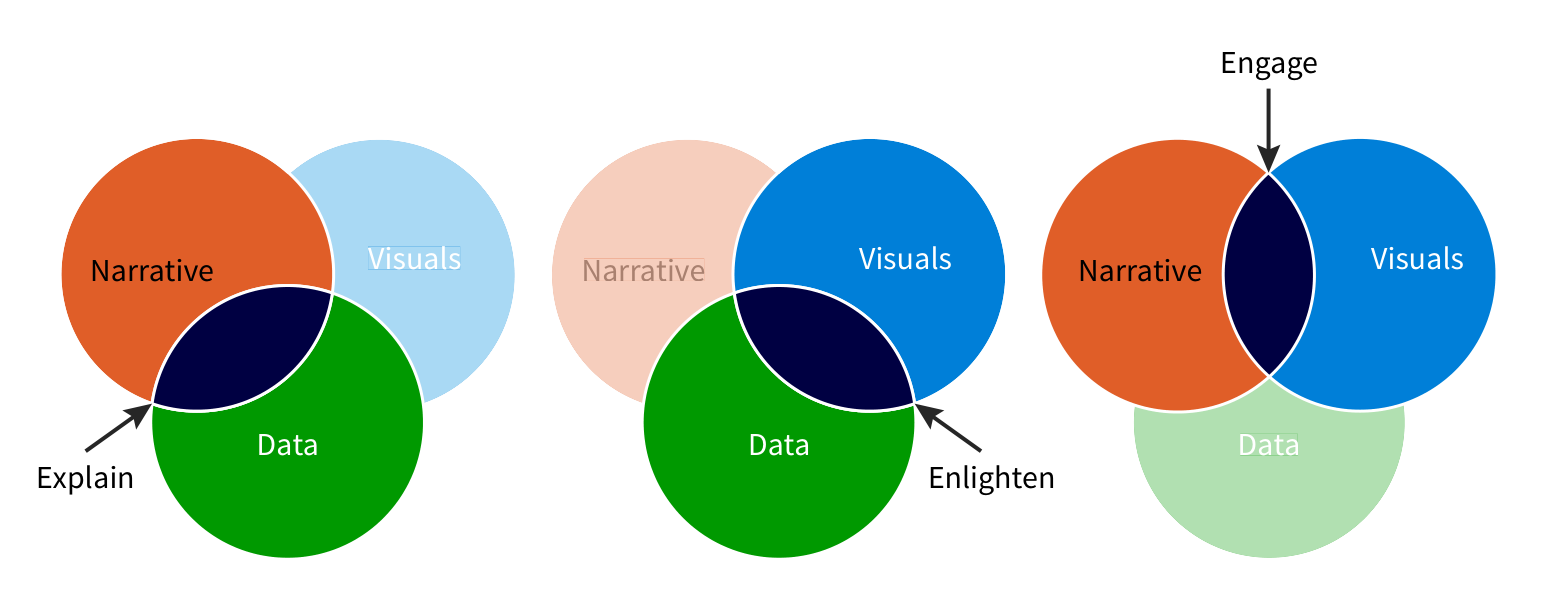
\includegraphics[width=0.95\textwidth,height=0.75\textheight,keepaspectratio]{../textbookForPractice/Figures/Ch_09/ILLUSTRATION 9.5.png}
    \end{figure}
\end{frame}

\begin{frame}{ILLUSTRATION 9.6}

    \begin{figure}[h]
        \centering
        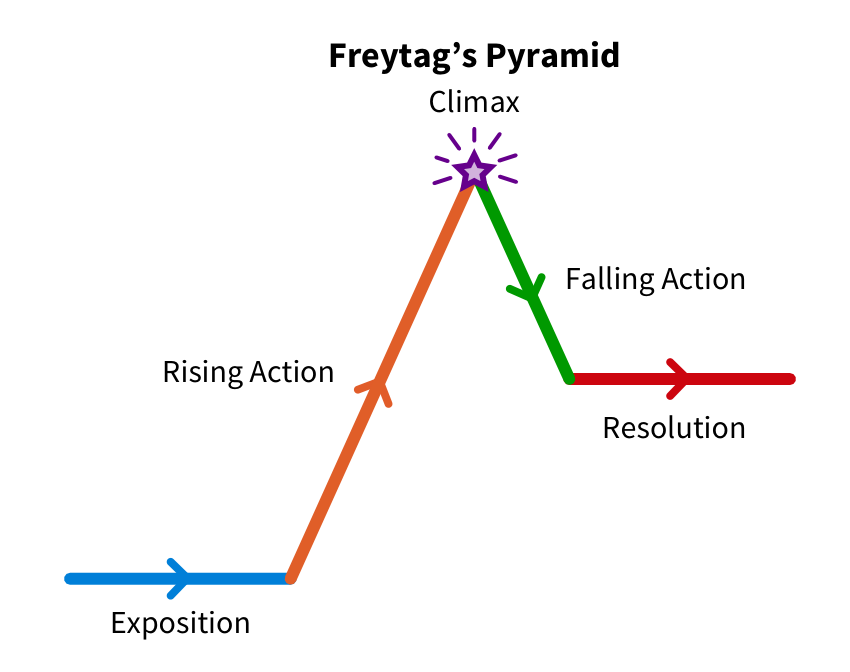
\includegraphics[width=0.95\textwidth,height=0.75\textheight,keepaspectratio]{../textbookForPractice/Figures/Ch_09/ILLUSTRATION 9.6.png}
    \end{figure}
\end{frame}

\begin{frame}{9.1 Kể Chuyện Bằng Dữ Liệu}
\begin{itemize}
    \item \textbf{Câu chuyện dữ liệu (Data Story) là gì?} Là sự giao thoa giữa dữ liệu, hình ảnh trực quan, và tường thuật logic.
    \item \textbf{Mục đích:} Giúp chuyển hóa những bảng số liệu khô khan thành các insight có thể hành động.
    \item Không chỉ là vẽ biểu đồ, mà là việc trả lời câu hỏi: \textit{"Dữ liệu này có ý nghĩa gì đối với công ty?"}
\end{itemize}
\end{frame}

\begin{frame}{ILLUSTRATION 9.7}

    \begin{figure}[h]
        \centering
        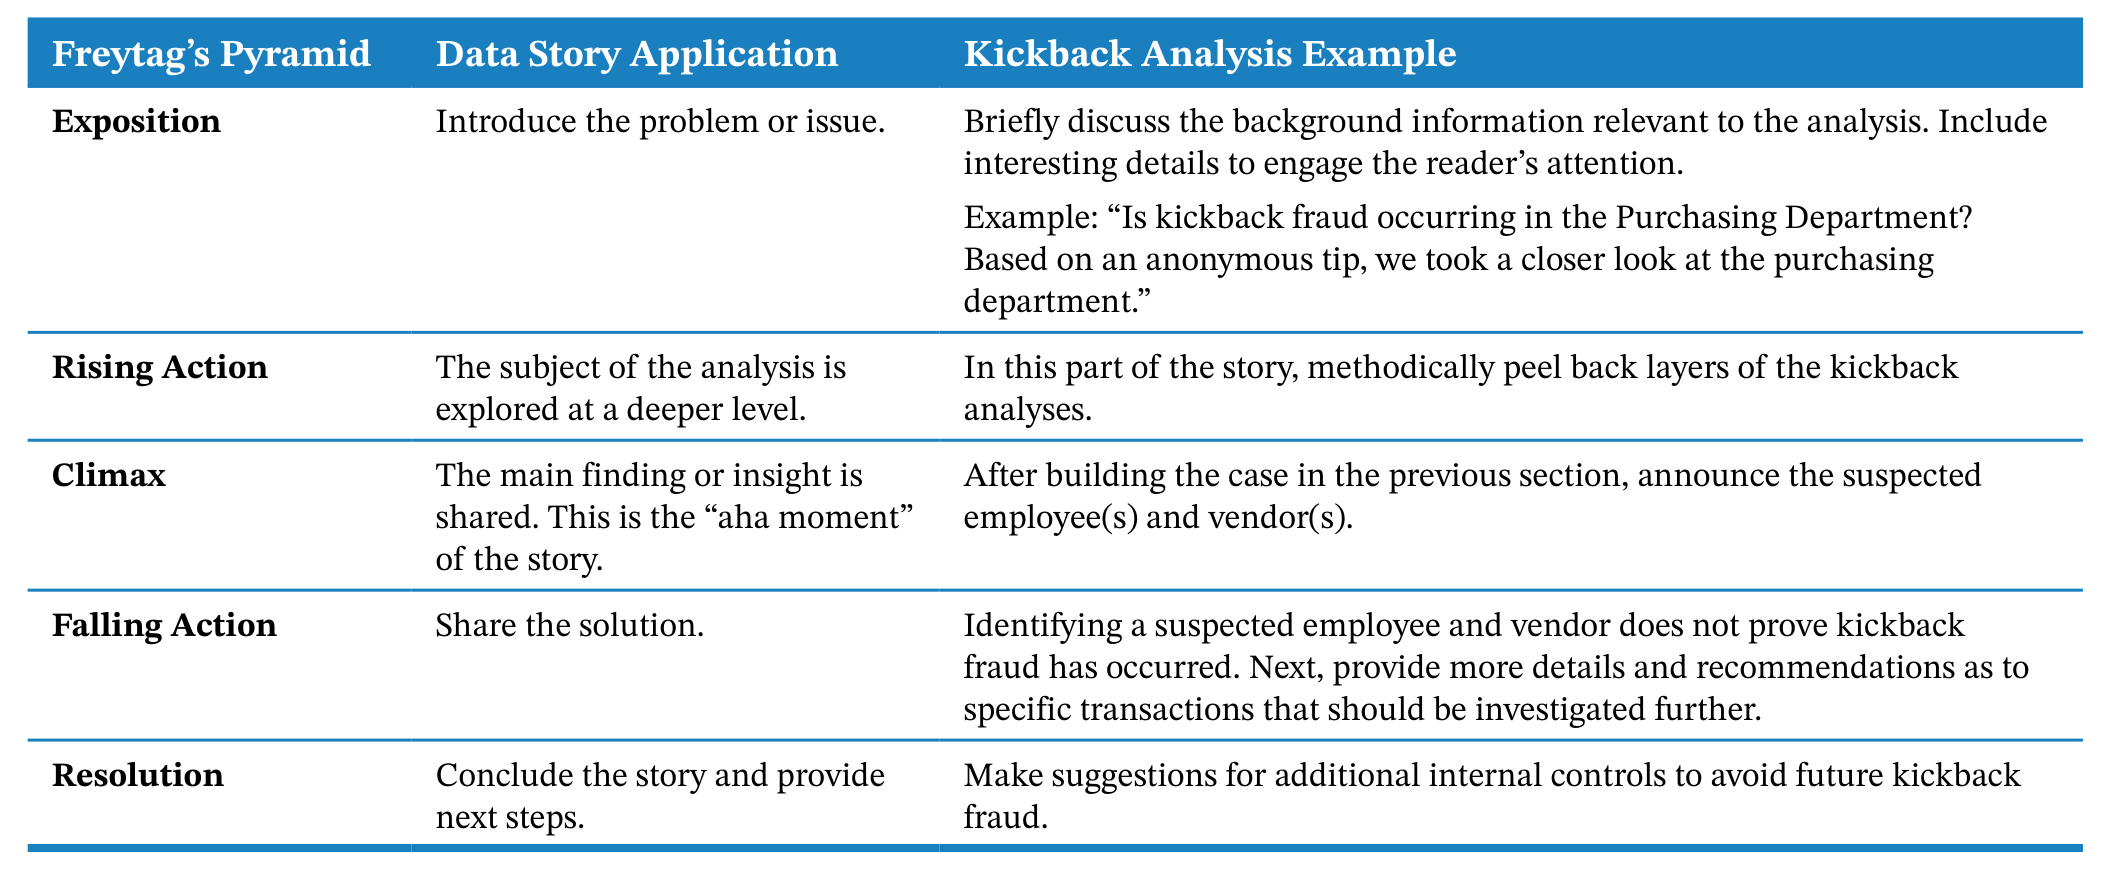
\includegraphics[width=0.95\textwidth,height=0.75\textheight,keepaspectratio]{../textbookForPractice/Figures/Ch_09/ILLUSTRATION 9.7.png}
    \end{figure}
\end{frame}

\begin{frame}{ILLUSTRATION 9.8}

    \begin{figure}[h]
        \centering
        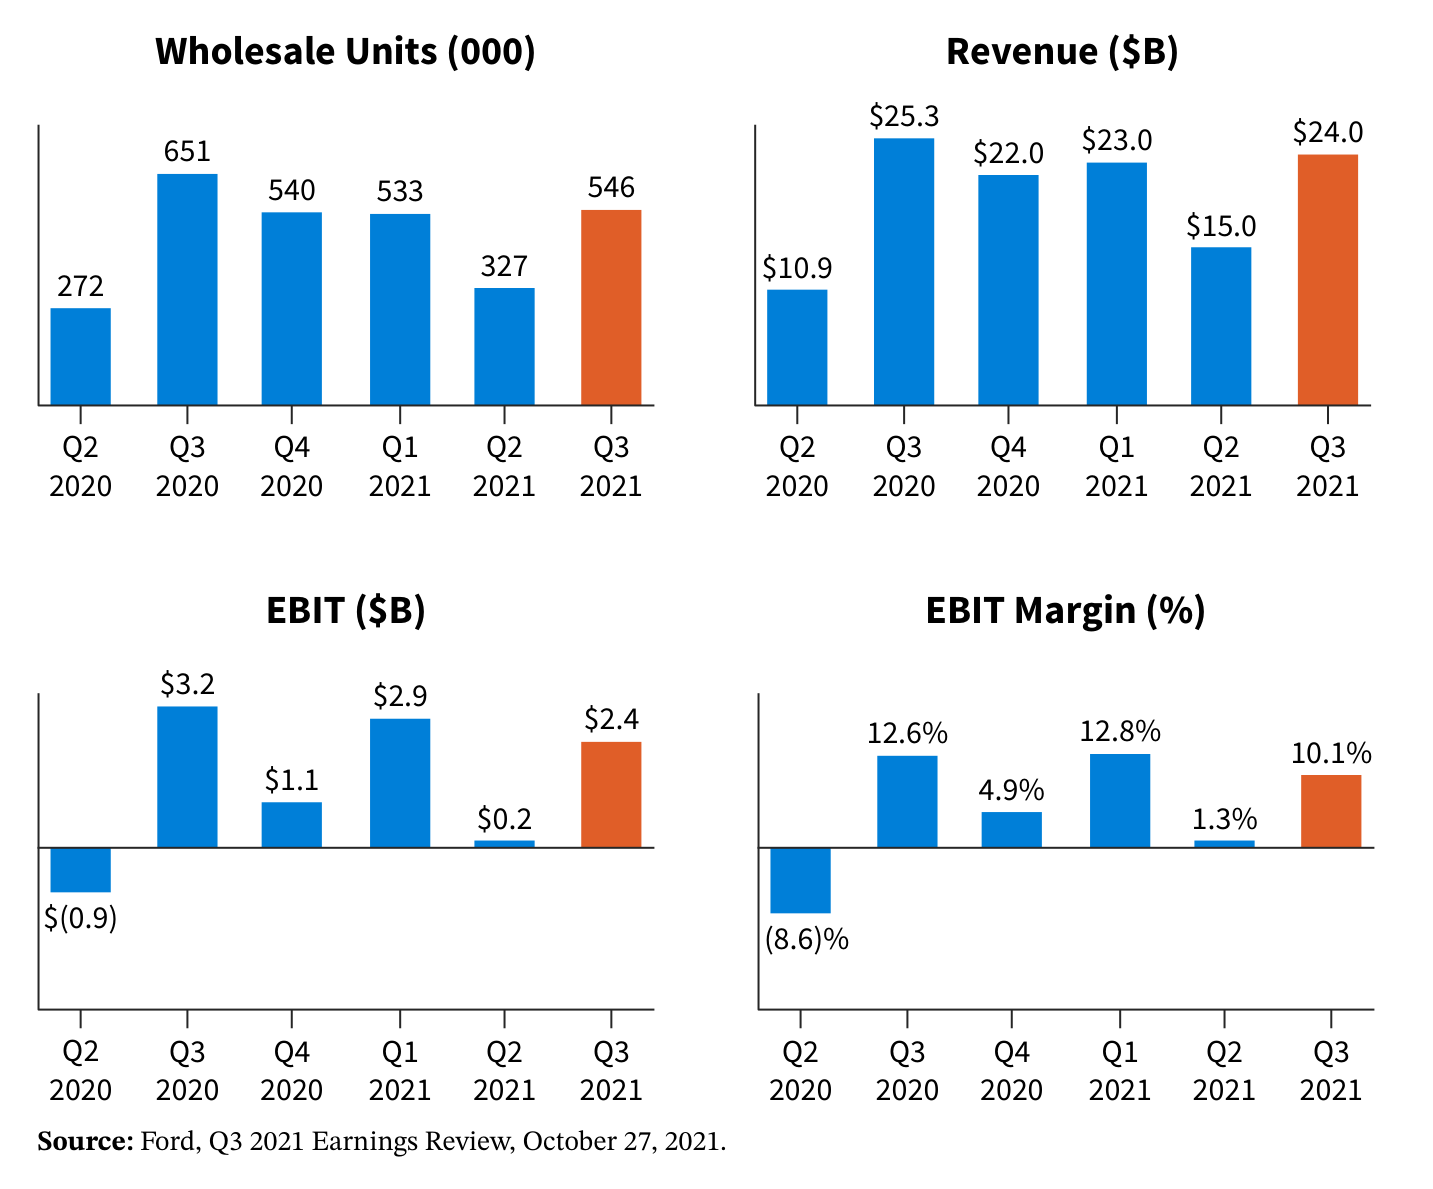
\includegraphics[width=0.95\textwidth,height=0.75\textheight,keepaspectratio]{../textbookForPractice/Figures/Ch_09/ILLUSTRATION 9.8.png}
    \end{figure}
\end{frame}

\begin{frame}{ILLUSTRATION 9.9}

    \begin{figure}[h]
        \centering
        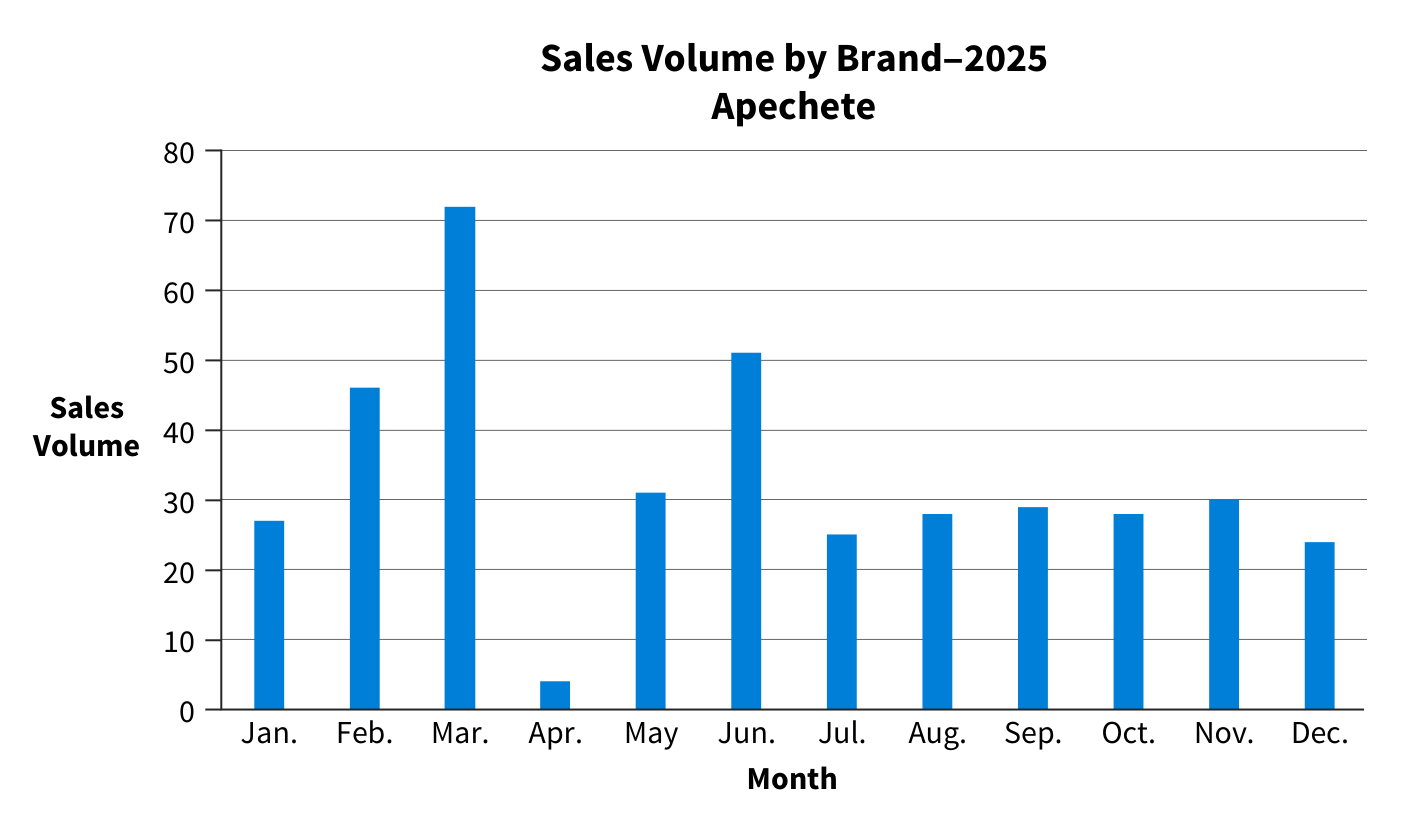
\includegraphics[width=0.95\textwidth,height=0.75\textheight,keepaspectratio]{../textbookForPractice/Figures/Ch_09/ILLUSTRATION 9.9.png}
    \end{figure}
\end{frame}

\begin{frame}{Phát triển Năng lực Dữ liệu}
\begin{itemize}
    \item \textbf{Data Literacy:} Khả năng đọc, làm việc, phân tích và tranh luận bằng dữ liệu.
    \item \textbf{Vai trò của Kế toán:} Là chuyên gia am hiểu hoạt động tài chính, kế toán viên ở vị thế lý tưởng nhất để trở thành "người kể chuyện" bằng dữ liệu cho Ban Giám đốc.
\end{itemize}
\end{frame}

\begin{frame}{ILLUSTRATION 9.10}

    \begin{figure}[h]
        \centering
        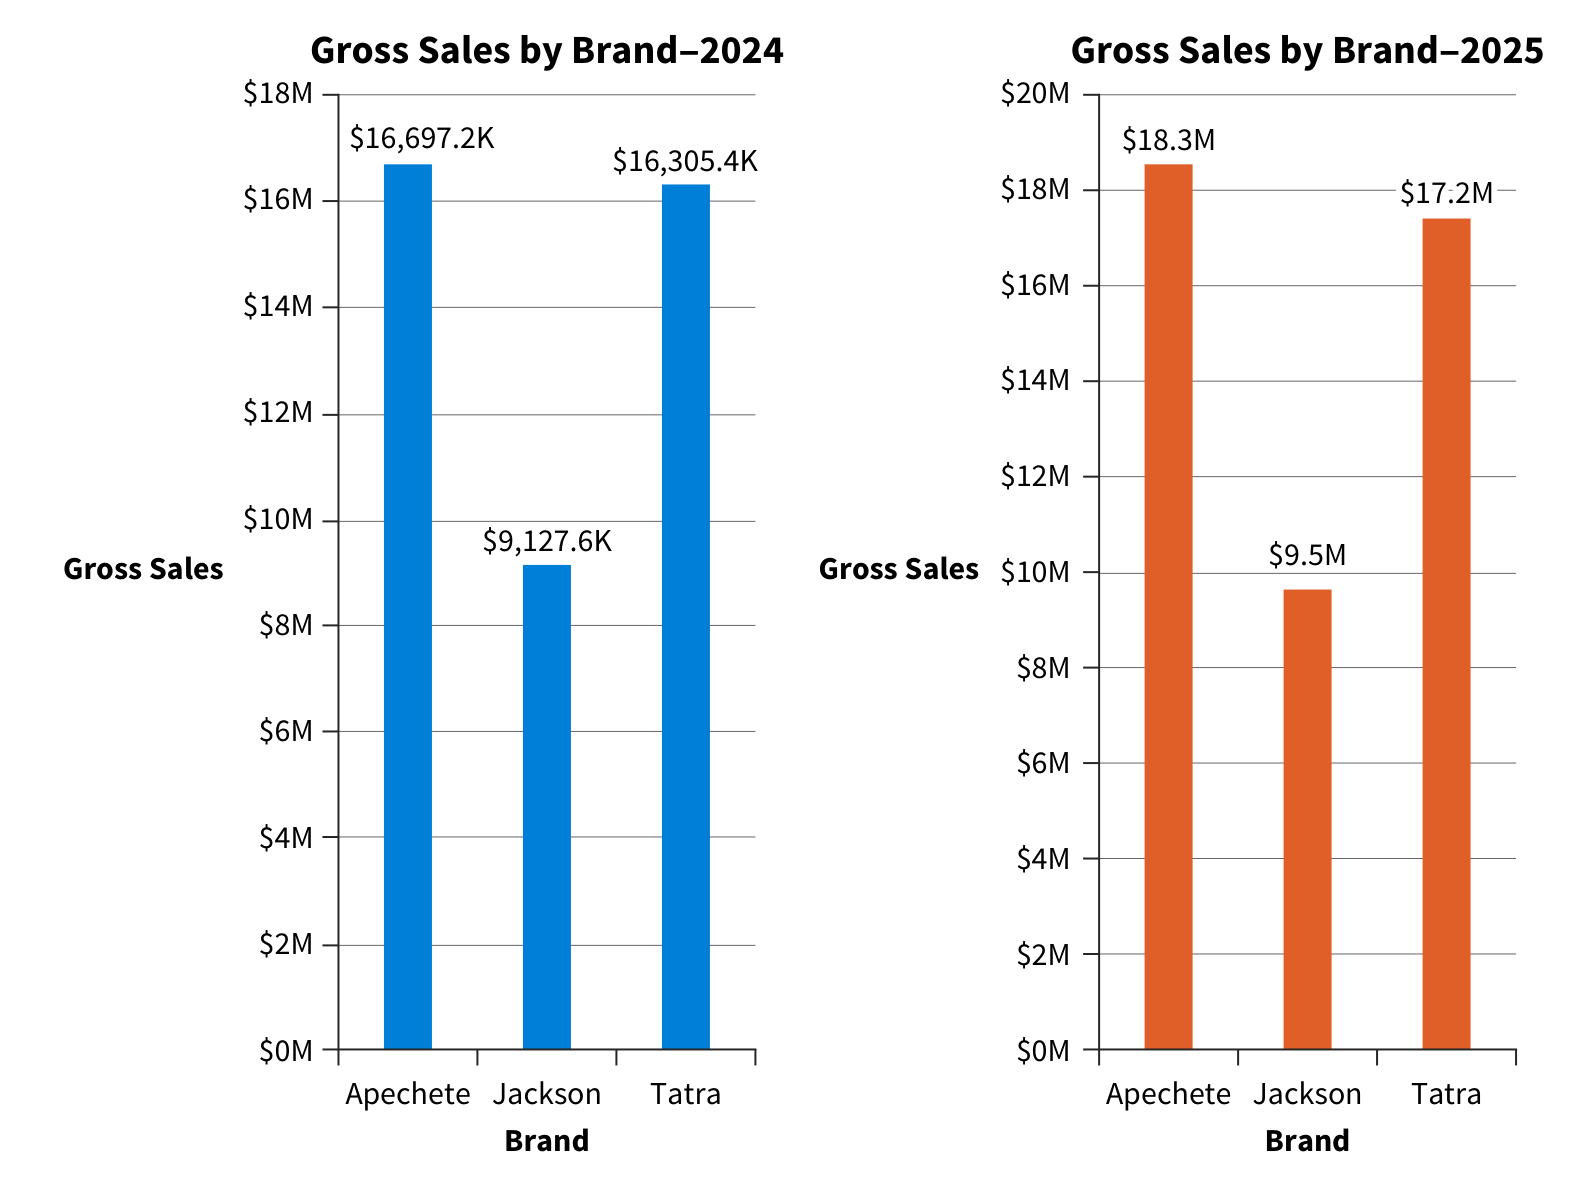
\includegraphics[width=0.95\textwidth,height=0.75\textheight,keepaspectratio]{../textbookForPractice/Figures/Ch_09/ILLUSTRATION 9.10.png}
    \end{figure}
\end{frame}

\begin{frame}{ILLUSTRATION 9.11}

    \begin{figure}[h]
        \centering
        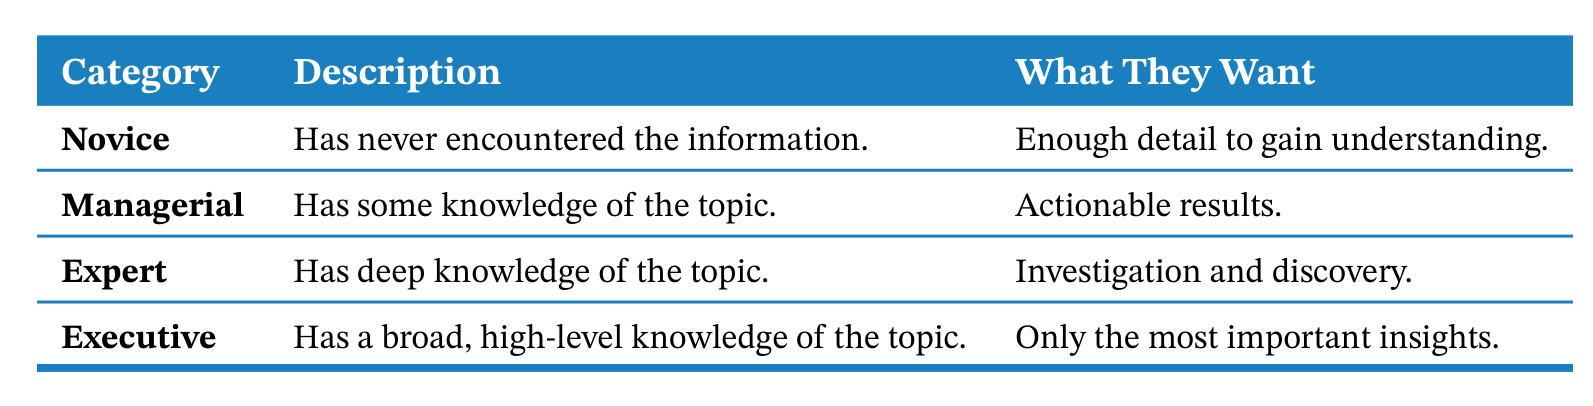
\includegraphics[width=0.95\textwidth,height=0.75\textheight,keepaspectratio]{../textbookForPractice/Figures/Ch_09/ILLUSTRATION 9.11.png}
    \end{figure}
\end{frame}

\begin{frame}{ILLUSTRATION 9.12}

    \begin{figure}[h]
        \centering
        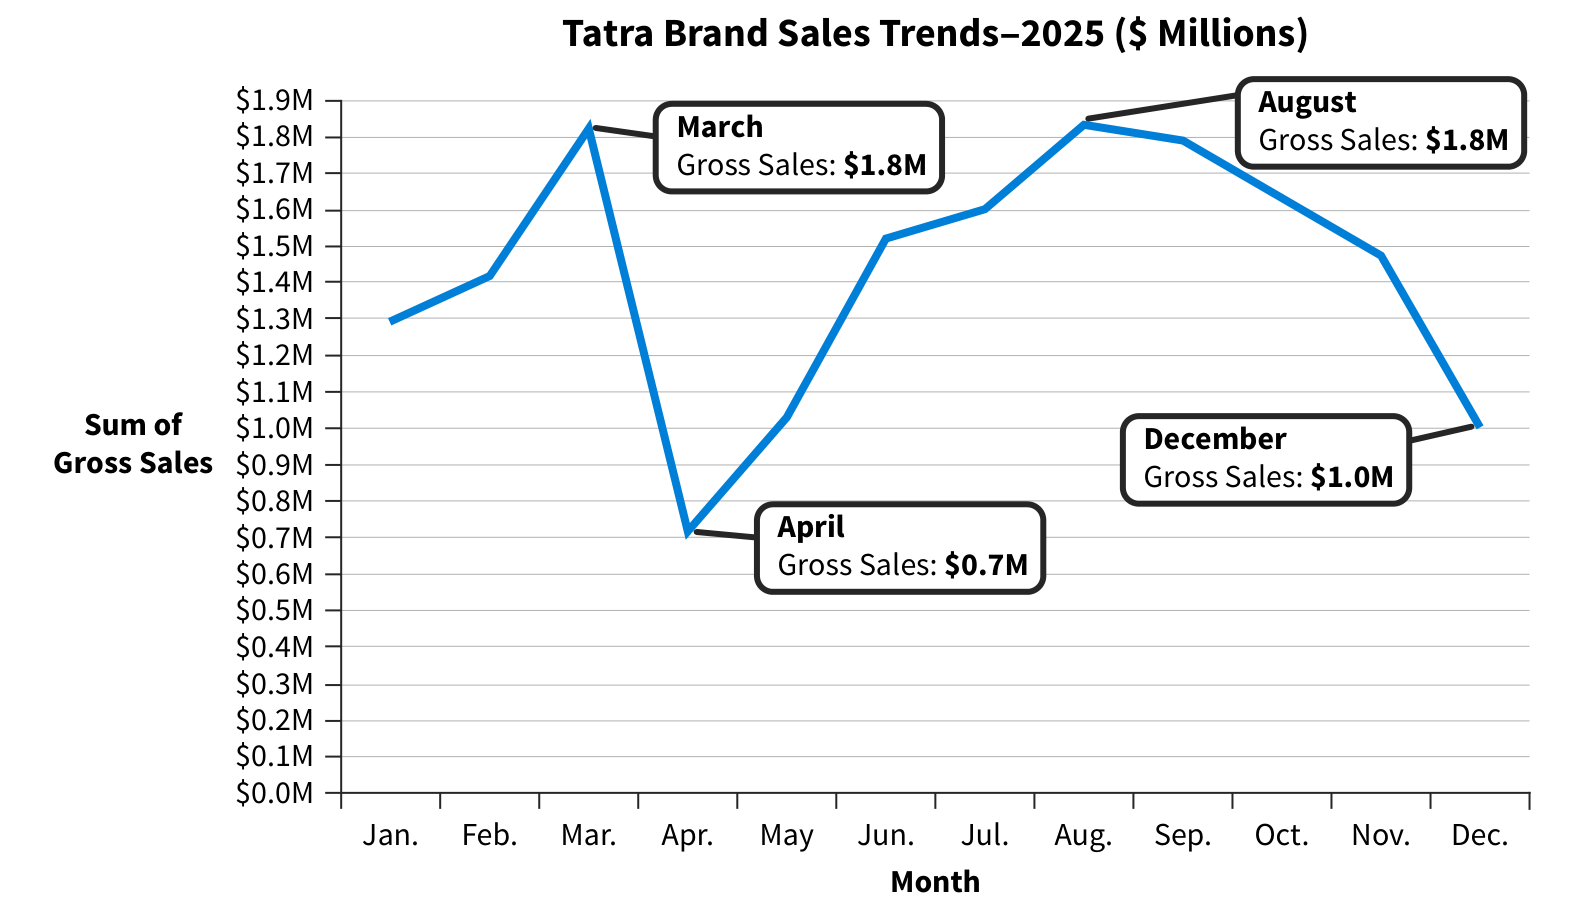
\includegraphics[width=0.95\textwidth,height=0.75\textheight,keepaspectratio]{../textbookForPractice/Figures/Ch_09/ILLUSTRATION 9.12.png}
    \end{figure}
\end{frame}

\begin{frame}{Kỹ thuật Xây dựng Câu chuyện}
\begin{itemize}
    \item \textbf{Bối cảnh (Context):} Dữ liệu này được thu thập khi nào? Nó phản ánh xu hướng gì?
    \item \textbf{Giao tiếp hiệu quả (Communicate Effectively):} Hãy trình bày rõ ràng thông điệp, đừng bắt khán giả phải tự tìm câu trả lời trong dữ liệu.
    \item Xác định cấu trúc cốt truyện: Bắt đầu bằng thực trạng, chỉ ra nút thắt (vấn đề) và đề xuất giải pháp.
\end{itemize}
\end{frame}

\begin{frame}{ILLUSTRATION 9.13}

    \begin{figure}[h]
        \centering
        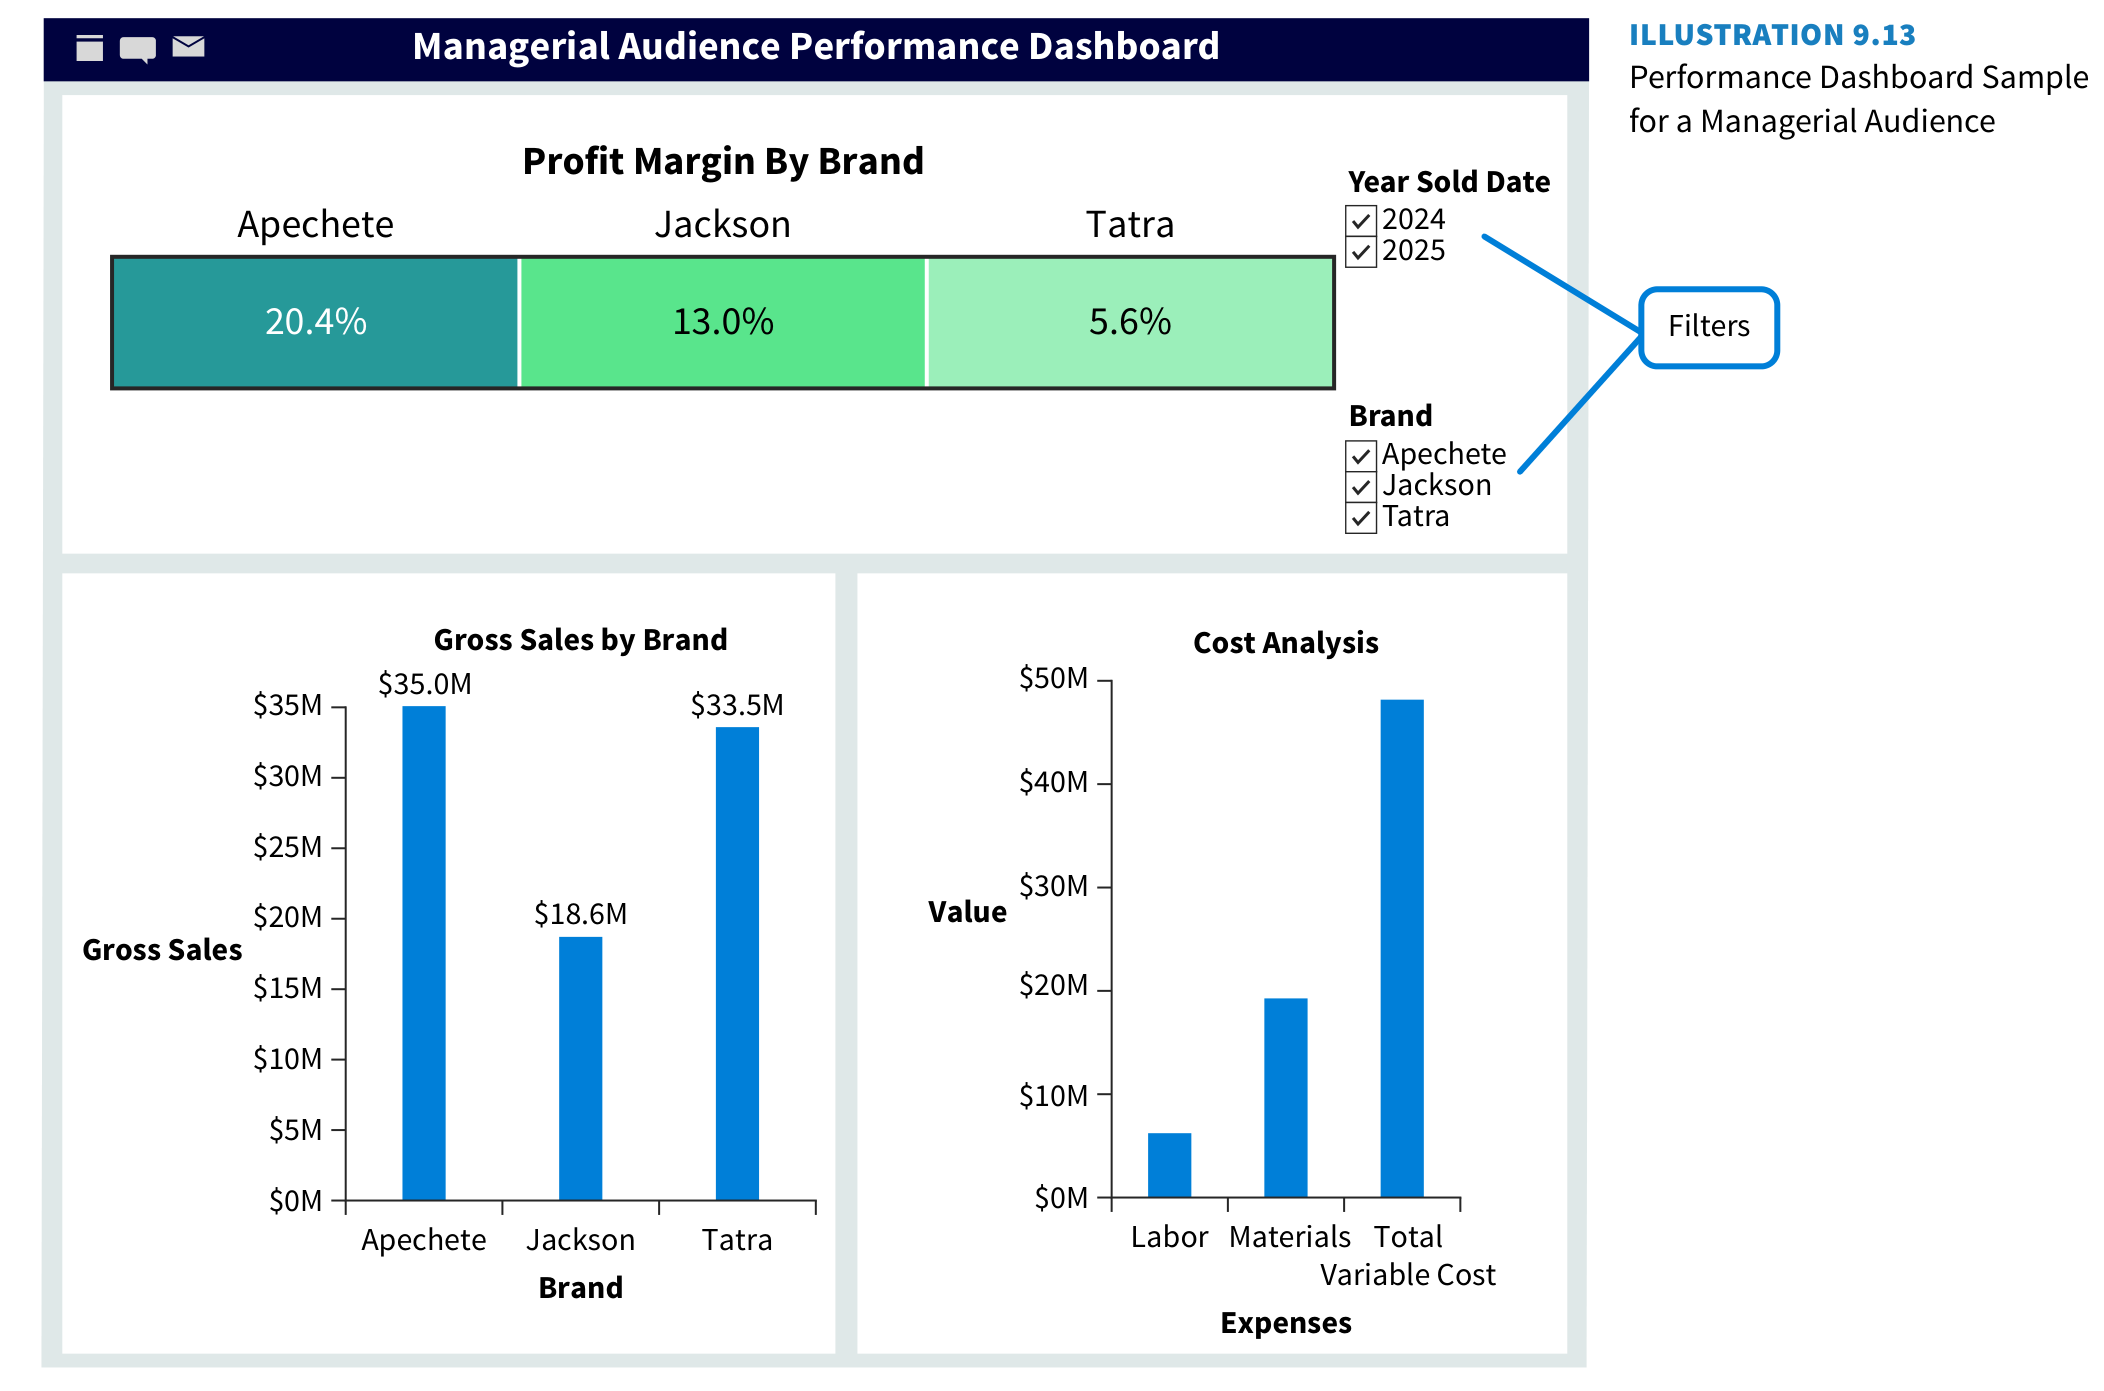
\includegraphics[width=0.95\textwidth,height=0.75\textheight,keepaspectratio]{../textbookForPractice/Figures/Ch_09/ILLUSTRATION 9.13.png}
    \end{figure}
\end{frame}

\begin{frame}{ILLUSTRATION 9.14}

    \begin{figure}[h]
        \centering
        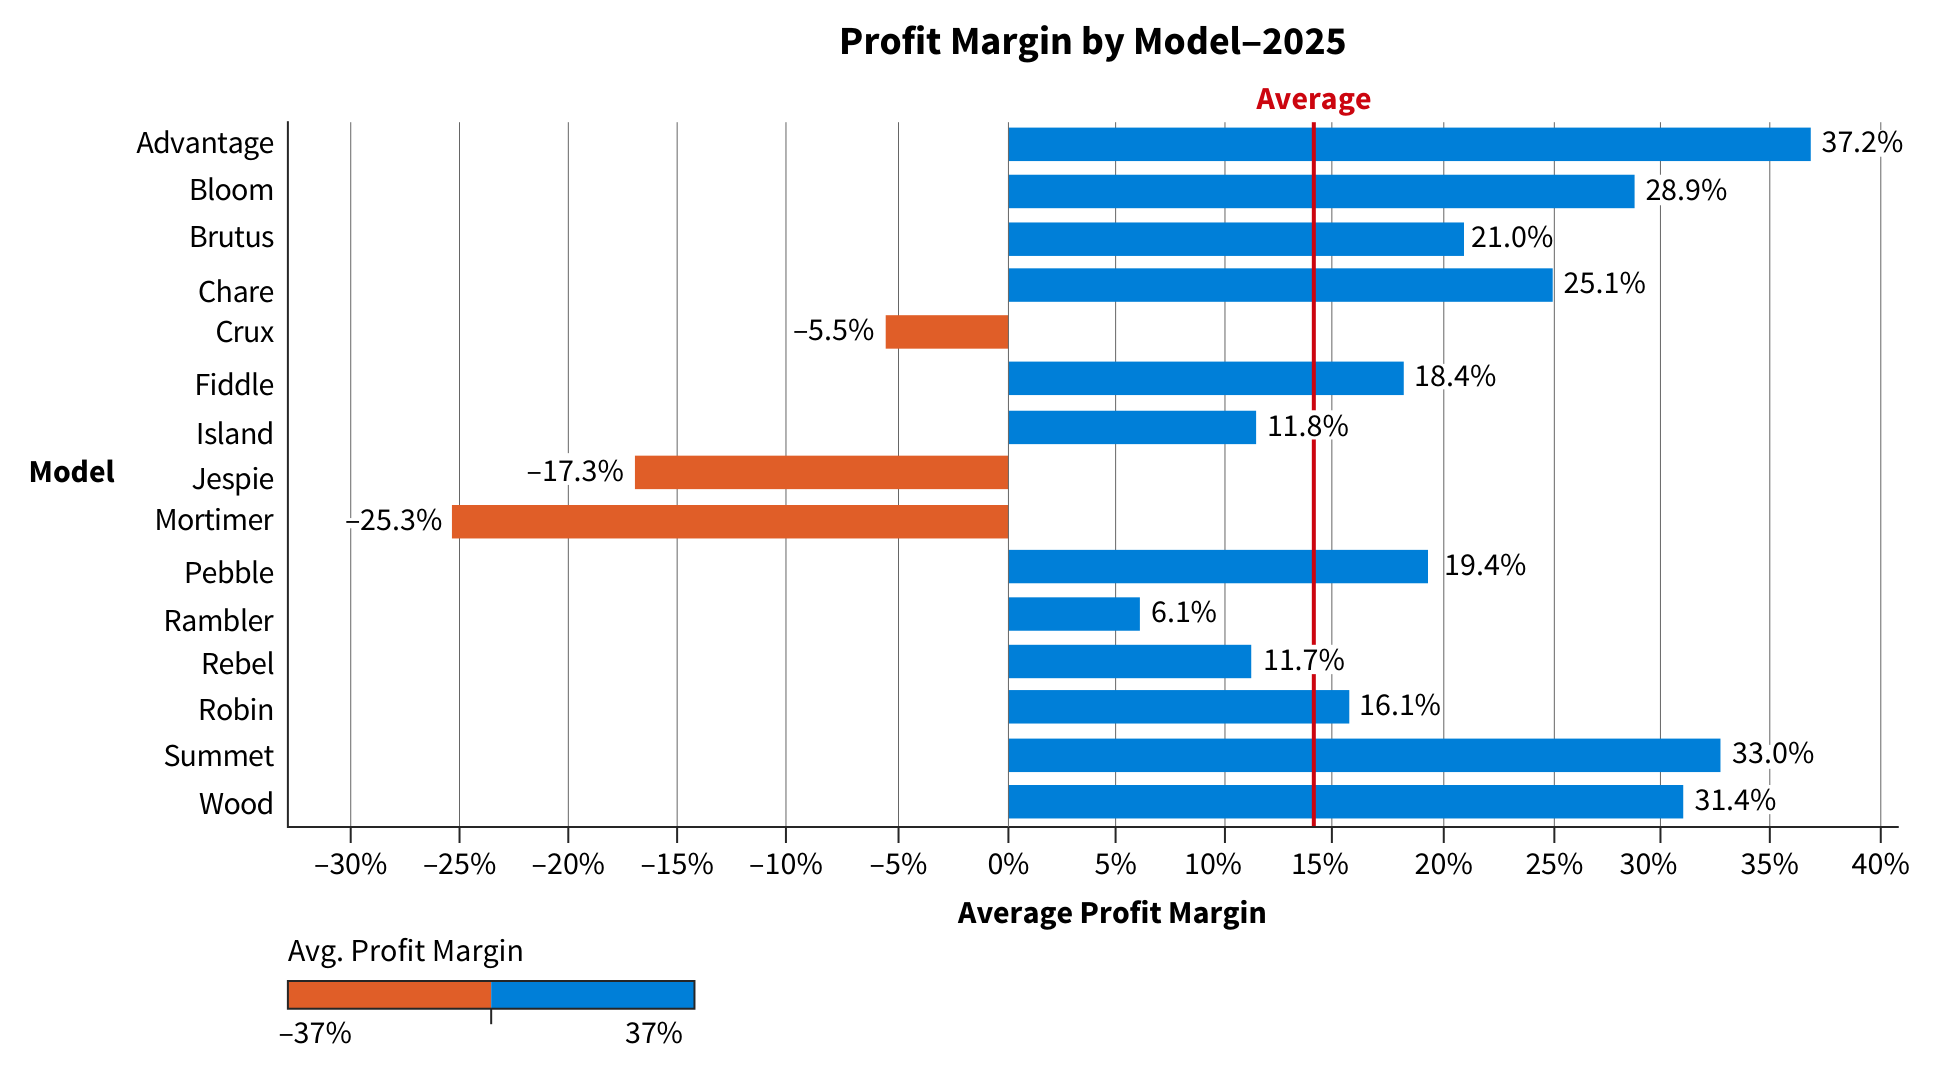
\includegraphics[width=0.95\textwidth,height=0.75\textheight,keepaspectratio]{../textbookForPractice/Figures/Ch_09/ILLUSTRATION 9.14.png}
    \end{figure}
\end{frame}

\begin{frame}{ILLUSTRATION 9.15}

    \begin{figure}[h]
        \centering
        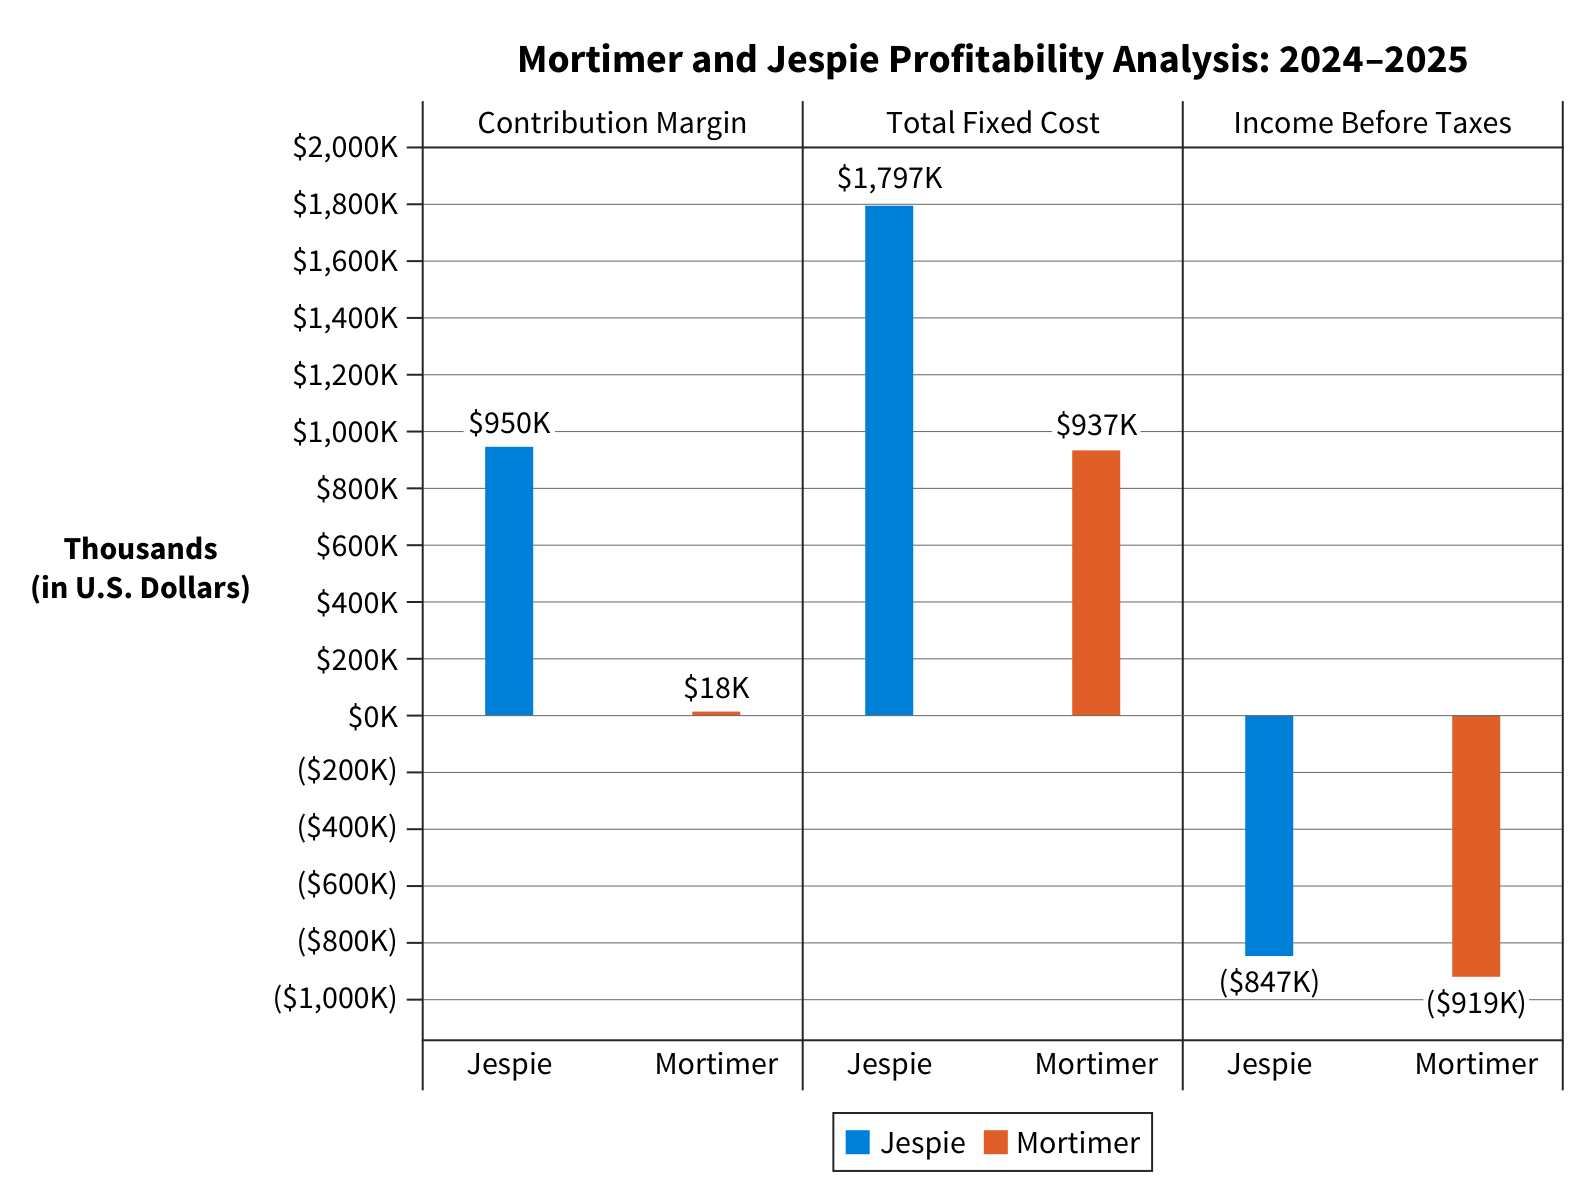
\includegraphics[width=0.95\textwidth,height=0.75\textheight,keepaspectratio]{../textbookForPractice/Figures/Ch_09/ILLUSTRATION 9.15.png}
    \end{figure}
\end{frame}

\begin{frame}{9.2 Quy Trình Tạo Trực Quan Hóa}
\begin{itemize}
    \item Trực quan hóa dữ liệu hiệu quả cần một quy trình tuần tự.
    \item \textbf{Quy trình 3 bước cốt lõi:}
    \begin{enumerate}
        \item Xác minh Dữ liệu (Verify the Data)
        \item Thấu hiểu Khán giả (Consider the Audience)
        \item Xác định Mục tiêu (Define the Objective)
    \end{enumerate}
\end{itemize}
\end{frame}

\begin{frame}{ILLUSTRATION 9.16}

    \begin{figure}[h]
        \centering
        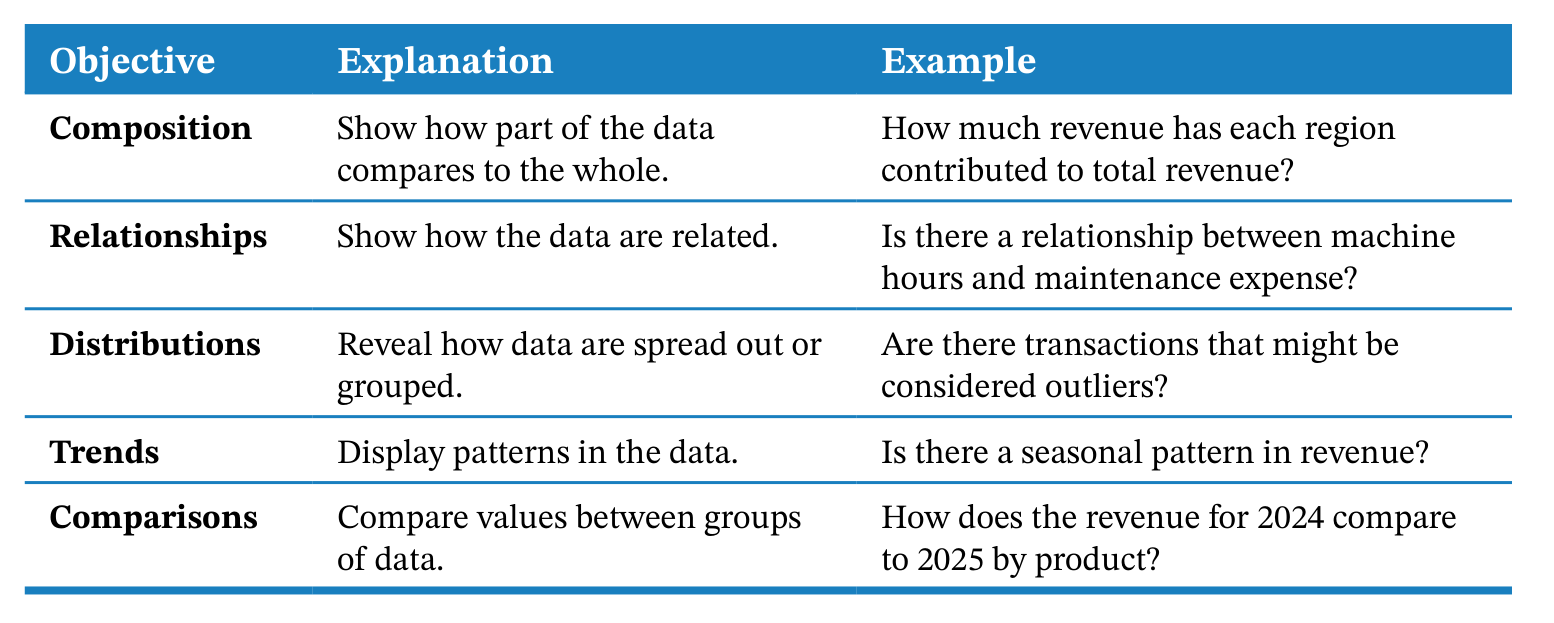
\includegraphics[width=0.95\textwidth,height=0.75\textheight,keepaspectratio]{../textbookForPractice/Figures/Ch_09/ILLUSTRATION 9.16.png}
    \end{figure}
\end{frame}

\begin{frame}{ILLUSTRATION 9.17}

    \begin{figure}[h]
        \centering
        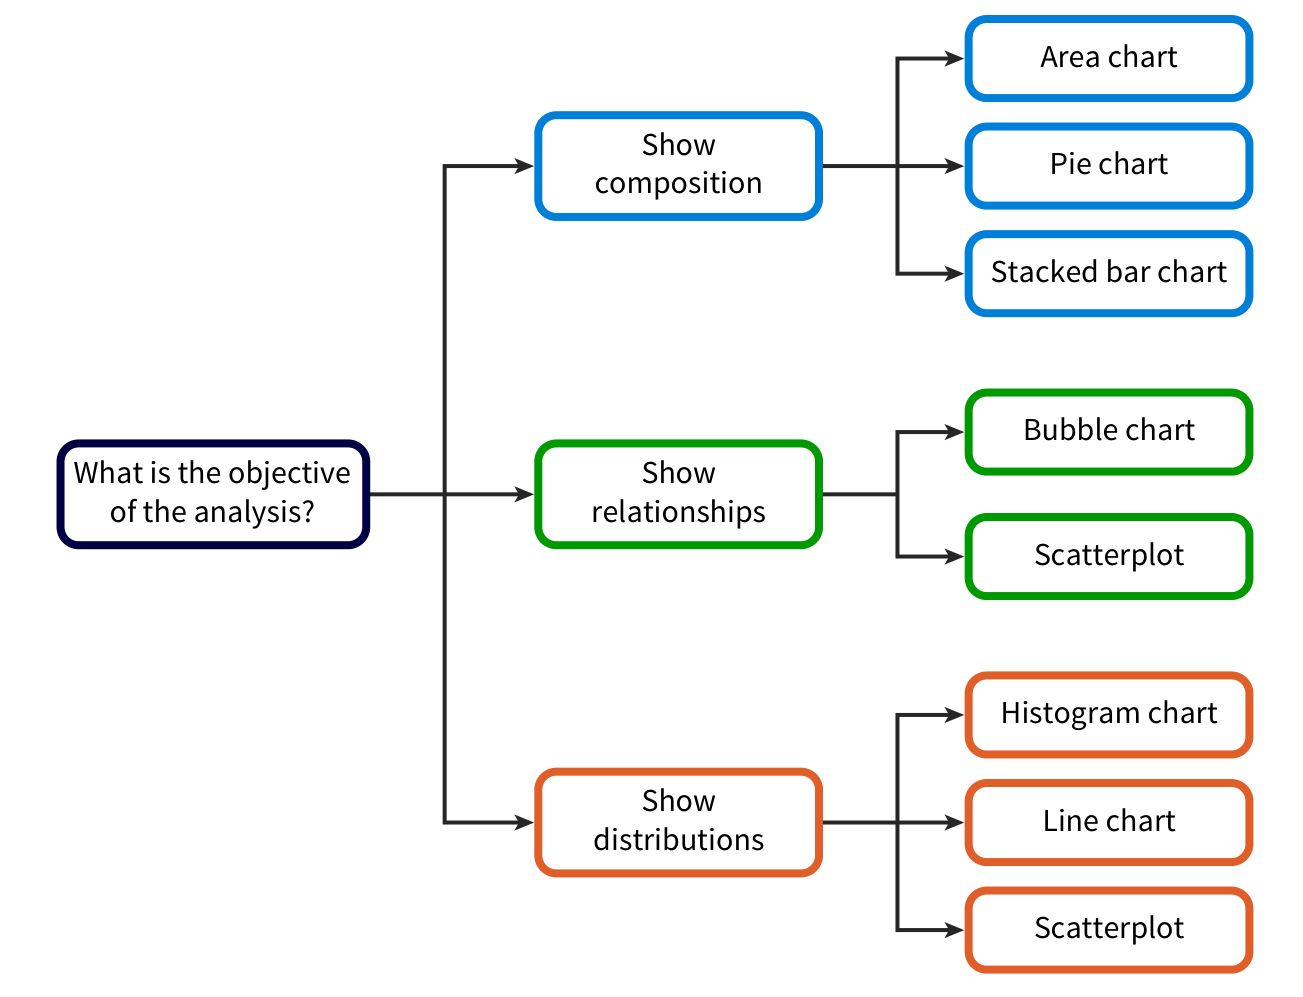
\includegraphics[width=0.95\textwidth,height=0.75\textheight,keepaspectratio]{../textbookForPractice/Figures/Ch_09/ILLUSTRATION 9.17.png}
    \end{figure}
\end{frame}

\begin{frame}{ILLUSTRATION 9.18}

    \begin{figure}[h]
        \centering
        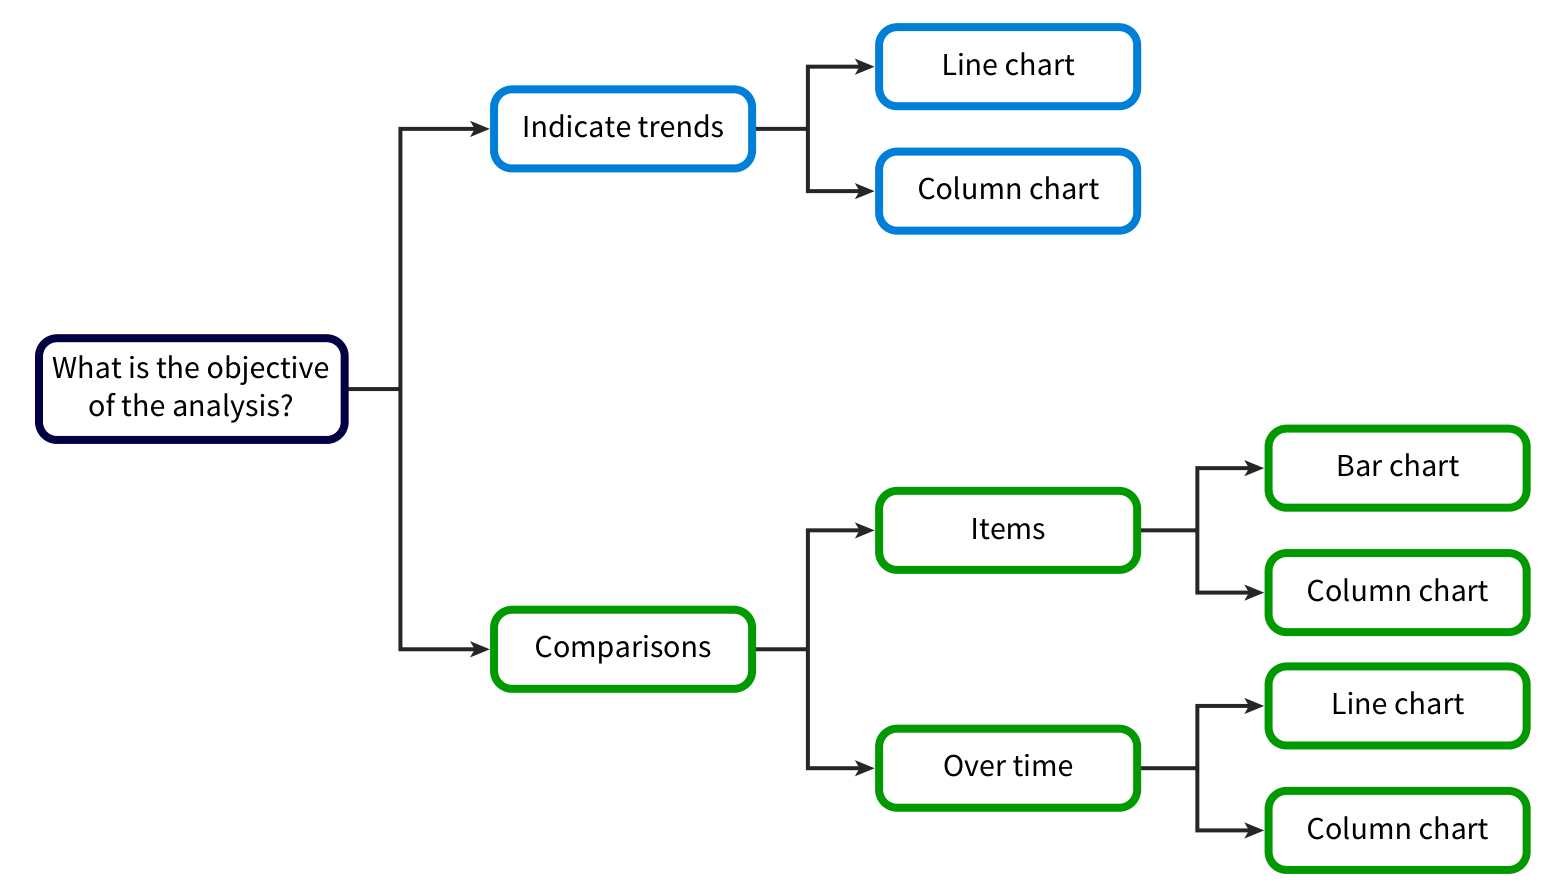
\includegraphics[width=0.95\textwidth,height=0.75\textheight,keepaspectratio]{../textbookForPractice/Figures/Ch_09/ILLUSTRATION 9.18.png}
    \end{figure}
\end{frame}

\begin{frame}{Bước 1 \& 2: Xác minh \& Thấu hiểu Khán giả}
\begin{itemize}
    \item \textbf{Xác minh Dữ liệu:} Đảm bảo tính chính xác, đầy đủ và hợp lệ. Dữ liệu sai sẽ dẫn đến biểu đồ sai (Garbage In, Garbage Out).
    \item \textbf{Thấu hiểu Khán giả:} Ai sẽ xem biểu đồ này? Họ có kiến thức chuyên môn về tài chính hay không? Mức độ chi tiết họ cần là bao nhiêu?
\end{itemize}
\end{frame}

\begin{frame}{ILLUSTRATION 9.19}

    \begin{figure}[h]
        \centering
        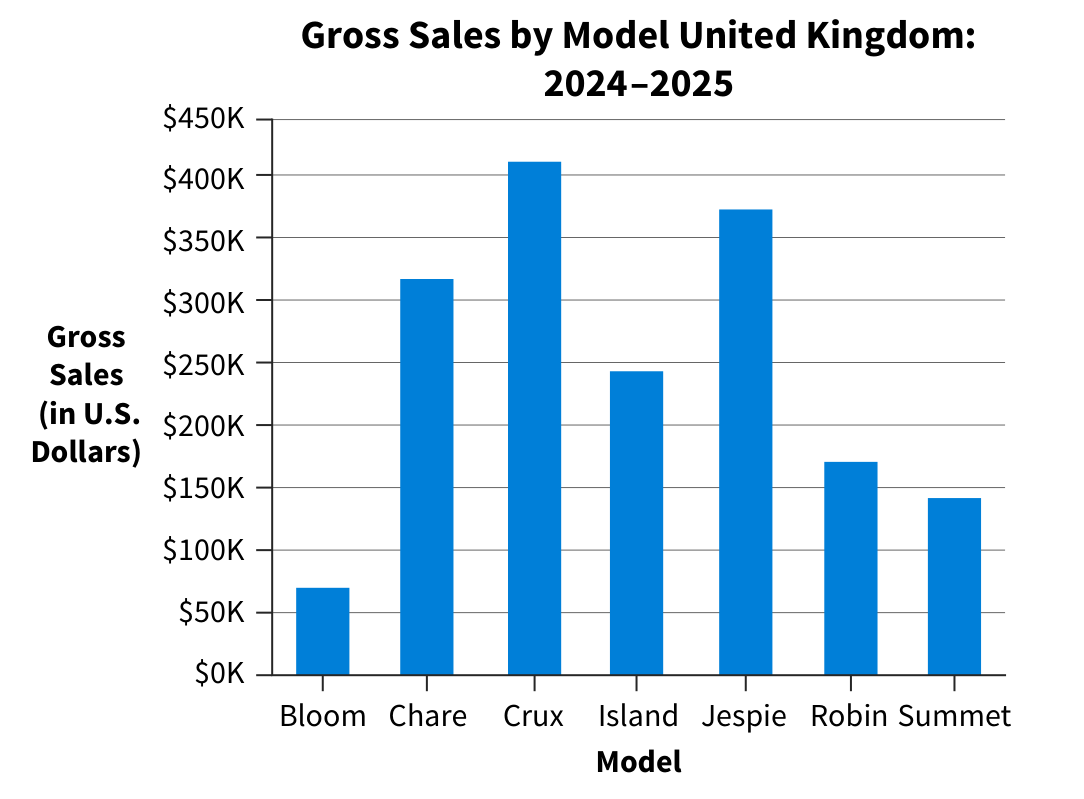
\includegraphics[width=0.95\textwidth,height=0.75\textheight,keepaspectratio]{../textbookForPractice/Figures/Ch_09/ILLUSTRATION 9.19.png}
    \end{figure}
\end{frame}

\begin{frame}{ILLUSTRATION 9.20}

    \begin{figure}[h]
        \centering
        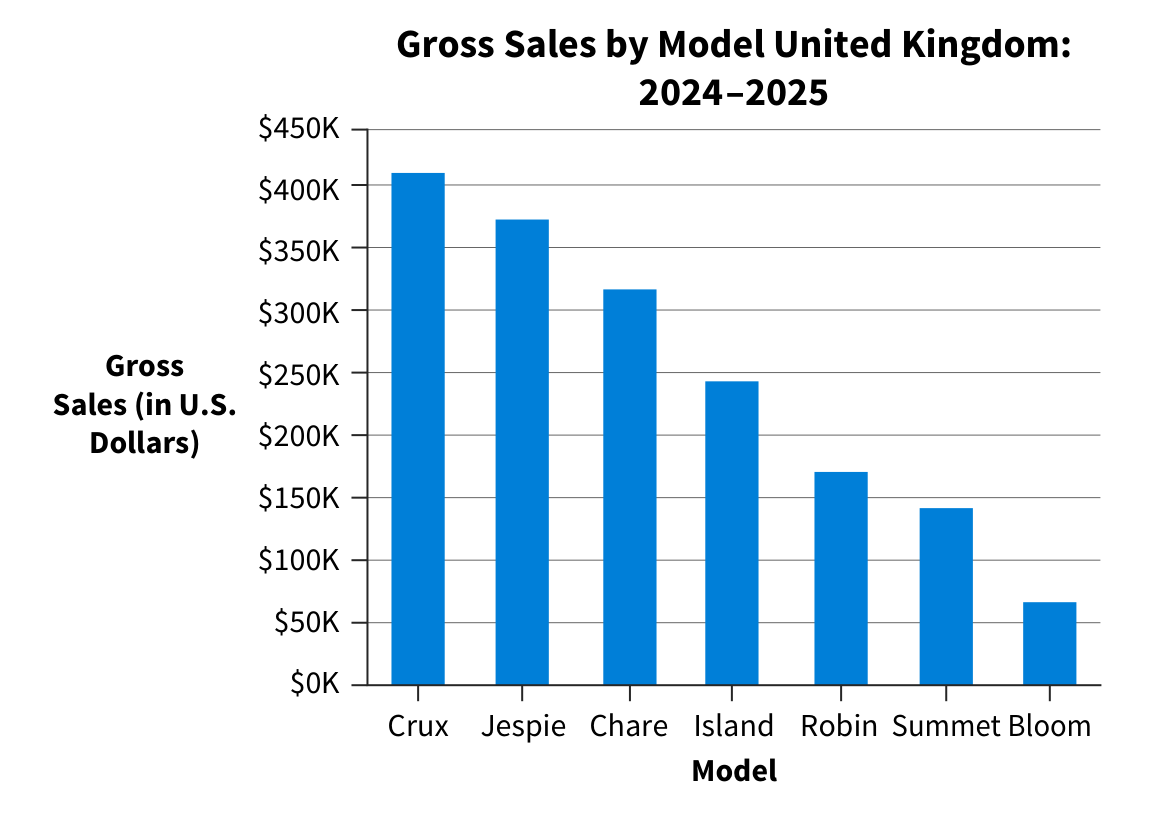
\includegraphics[width=0.95\textwidth,height=0.75\textheight,keepaspectratio]{../textbookForPractice/Figures/Ch_09/ILLUSTRATION 9.20.png}
    \end{figure}
\end{frame}

\begin{frame}{ILLUSTRATION 9.21}

    \begin{figure}[h]
        \centering
        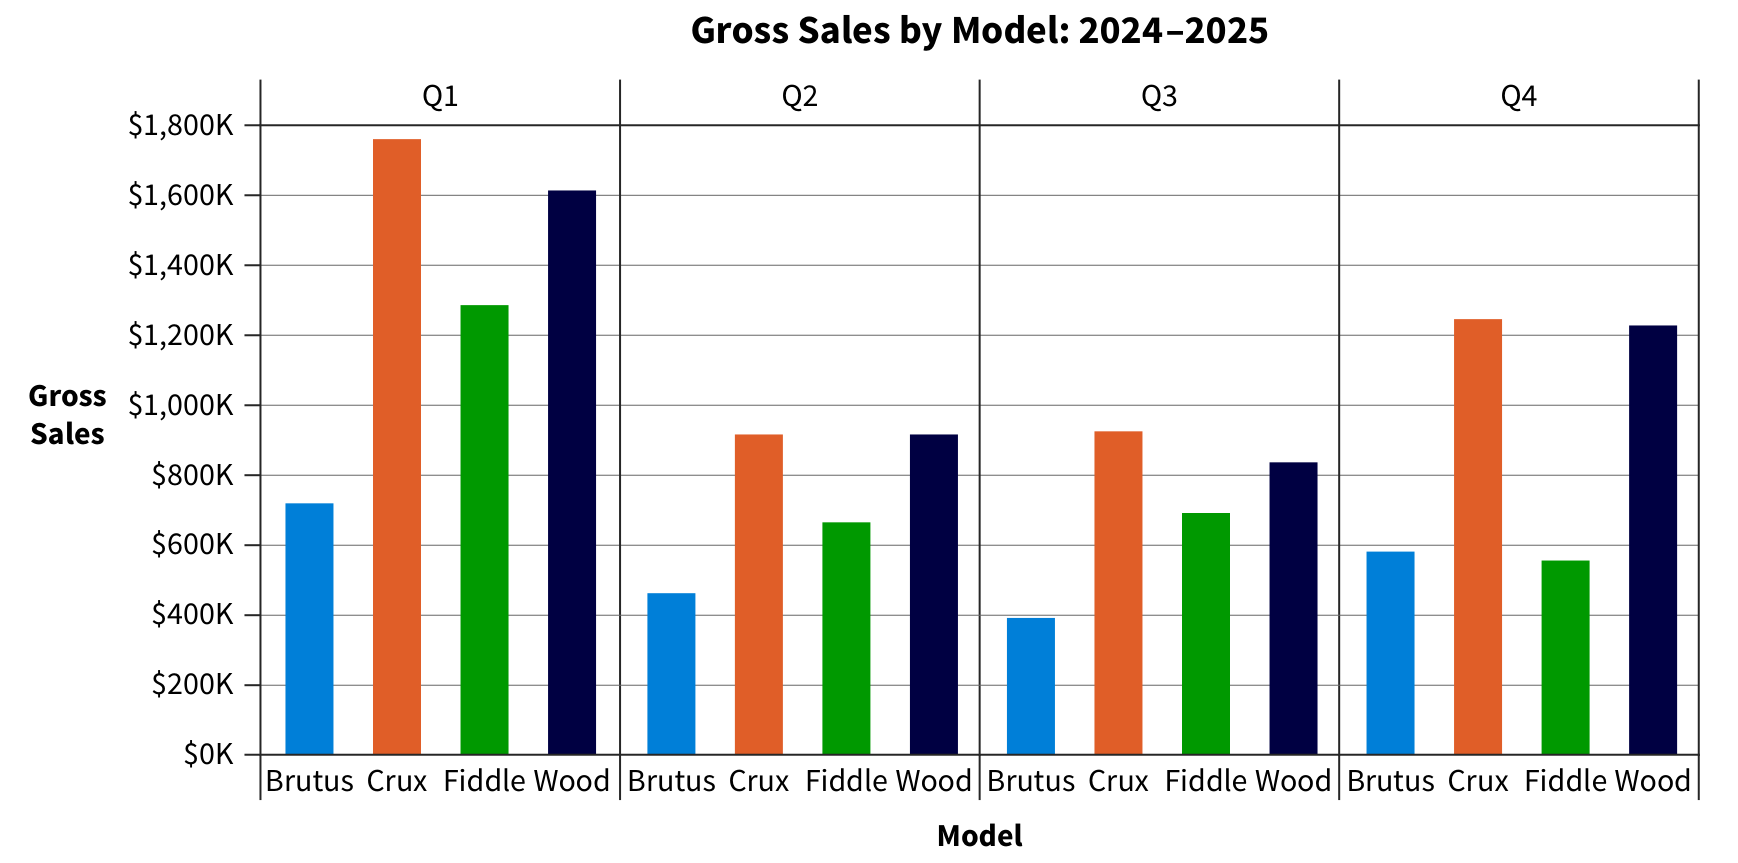
\includegraphics[width=0.95\textwidth,height=0.75\textheight,keepaspectratio]{../textbookForPractice/Figures/Ch_09/ILLUSTRATION 9.21.png}
    \end{figure}
\end{frame}

\begin{frame}{Bước 3: Xác định Mục tiêu (Define the Objective)}
\begin{itemize}
    \item \textbf{Mục tiêu:} Biểu đồ nhằm mục đích so sánh, chỉ ra xu hướng, hay hiển thị tỷ trọng?
    \item \textbf{Lựa chọn biểu đồ (Chart selection):} Phải chọn đúng biểu đồ phù hợp với mục tiêu.
    \begin{itemize}
        \item \textit{Ví dụ:} So sánh giữa các mục thì dùng Bar Chart. Xem xu hướng theo thời gian thì dùng Line Chart.
    \end{itemize}
\end{itemize}
\end{frame}

\begin{frame}{ILLUSTRATION 9.22}

    \begin{figure}[h]
        \centering
        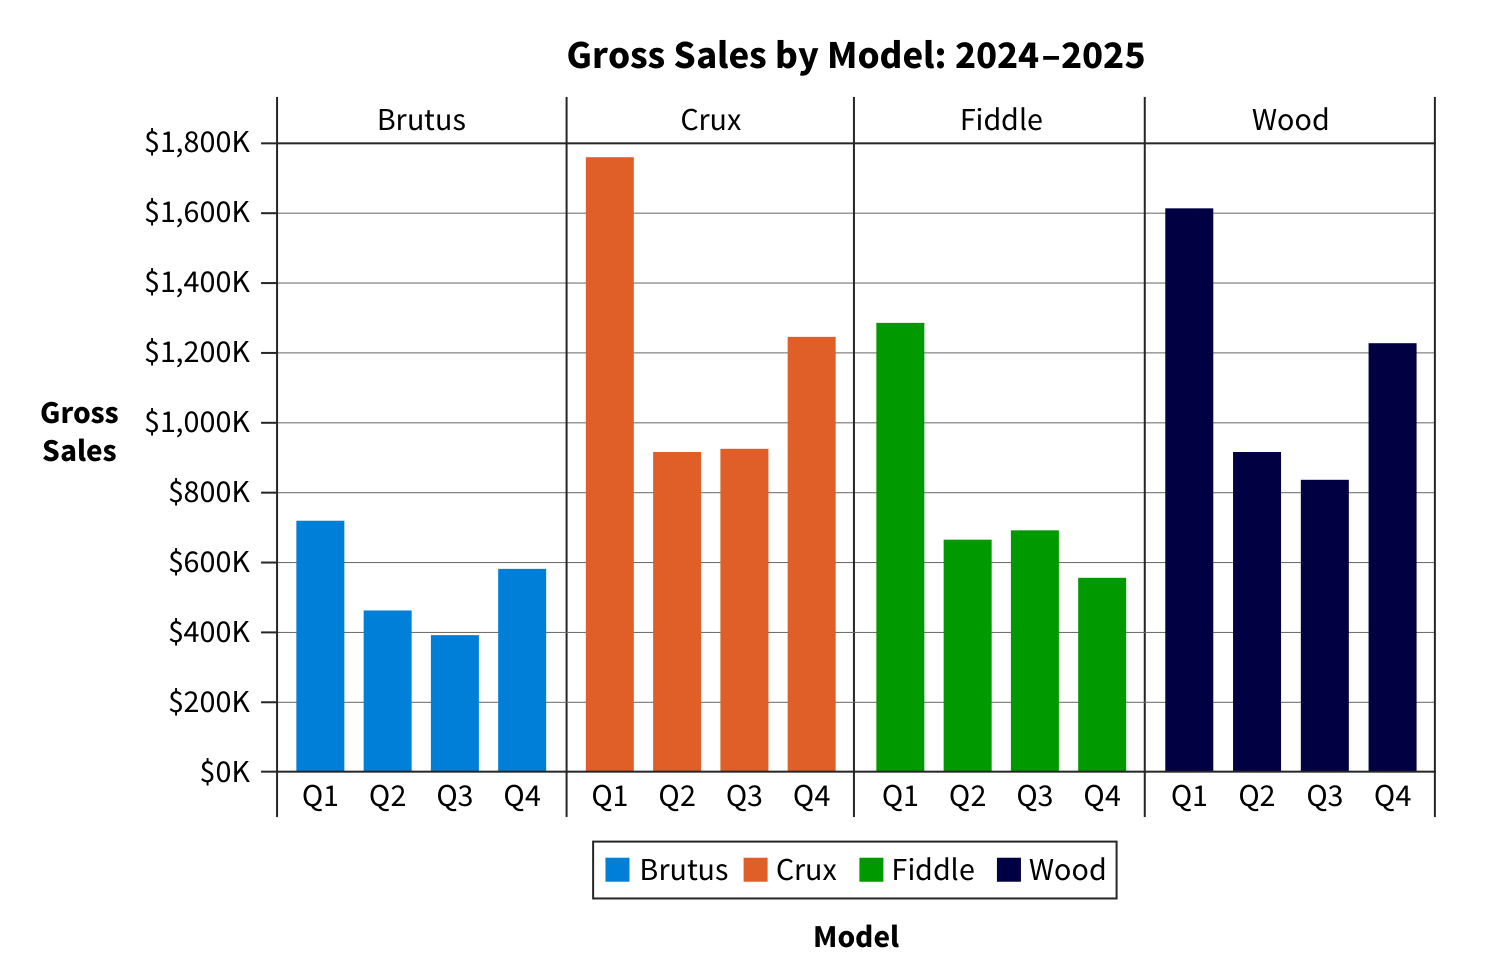
\includegraphics[width=0.95\textwidth,height=0.75\textheight,keepaspectratio]{../textbookForPractice/Figures/Ch_09/ILLUSTRATION 9.22.png}
    \end{figure}
\end{frame}

\begin{frame}{ILLUSTRATION 9.23}

    \begin{figure}[h]
        \centering
        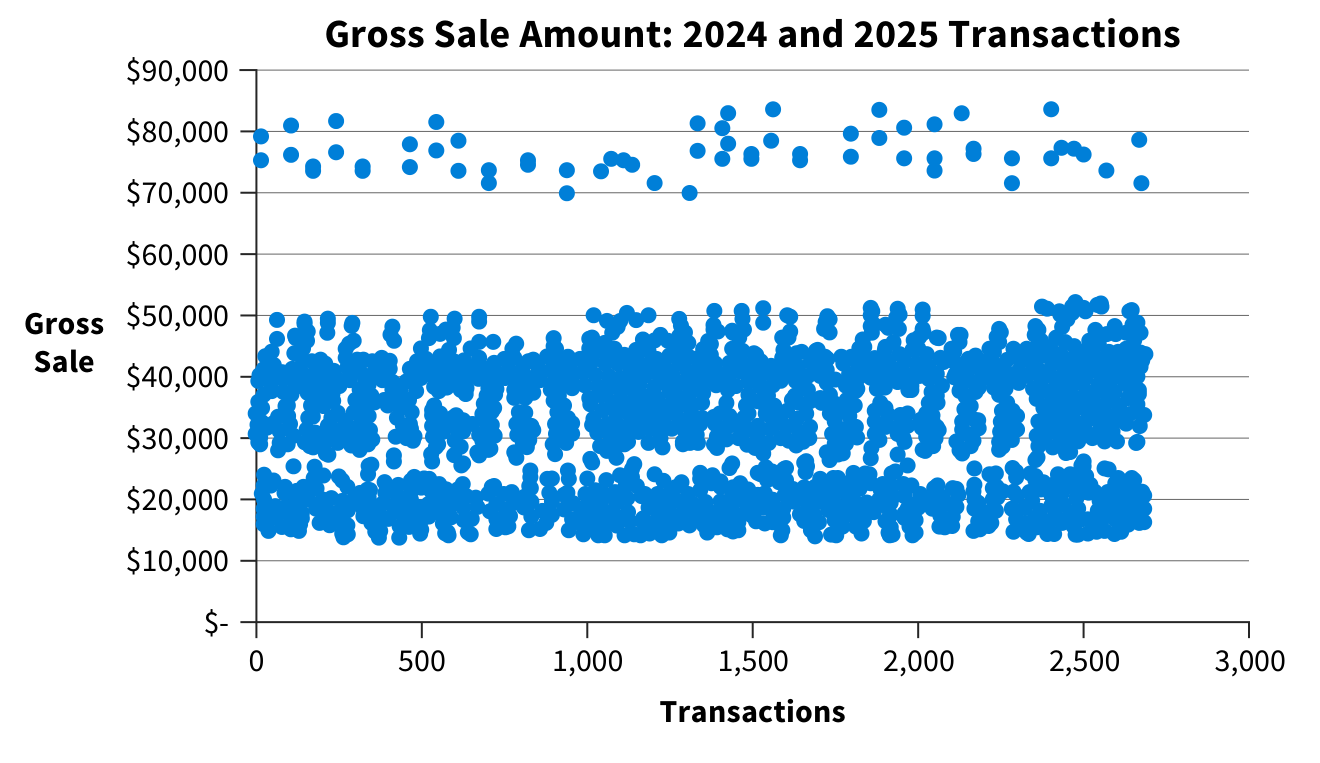
\includegraphics[width=0.95\textwidth,height=0.75\textheight,keepaspectratio]{../textbookForPractice/Figures/Ch_09/ILLUSTRATION 9.23.png}
    \end{figure}
\end{frame}

\begin{frame}{ILLUSTRATION 9.24}

    \begin{figure}[h]
        \centering
        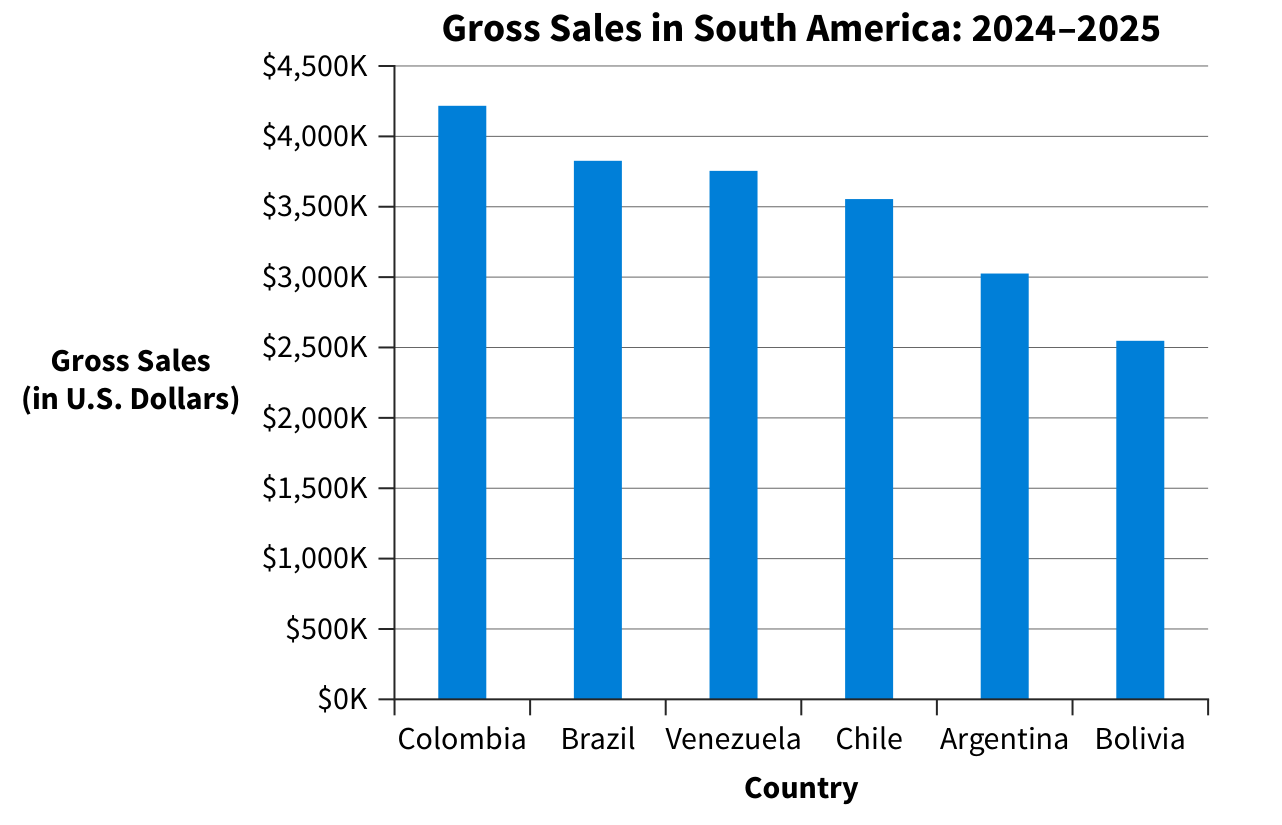
\includegraphics[width=0.95\textwidth,height=0.75\textheight,keepaspectratio]{../textbookForPractice/Figures/Ch_09/ILLUSTRATION 9.24.png}
    \end{figure}
\end{frame}

\begin{frame}{9.3 Đặc Điểm Trực Quan Hóa Hiệu Quả}
\begin{itemize}
    \item \textbf{Hiệu quả là gì?} Là khả năng truyền tải thông điệp nhanh nhất và ít gây nhầm lẫn nhất.
    \item \textbf{Nhận thức Thị giác (Visual Perception):} Não bộ con người được tối ưu hóa để xử lý hình ảnh và màu sắc thay vì các con số dạng văn bản.
    \item Chìa khóa: Khai thác sức mạnh của hệ thống thị giác để hướng sự chú ý của người xem.
\end{itemize}
\end{frame}

\begin{frame}{ILLUSTRATION 9.25}

    \begin{figure}[h]
        \centering
        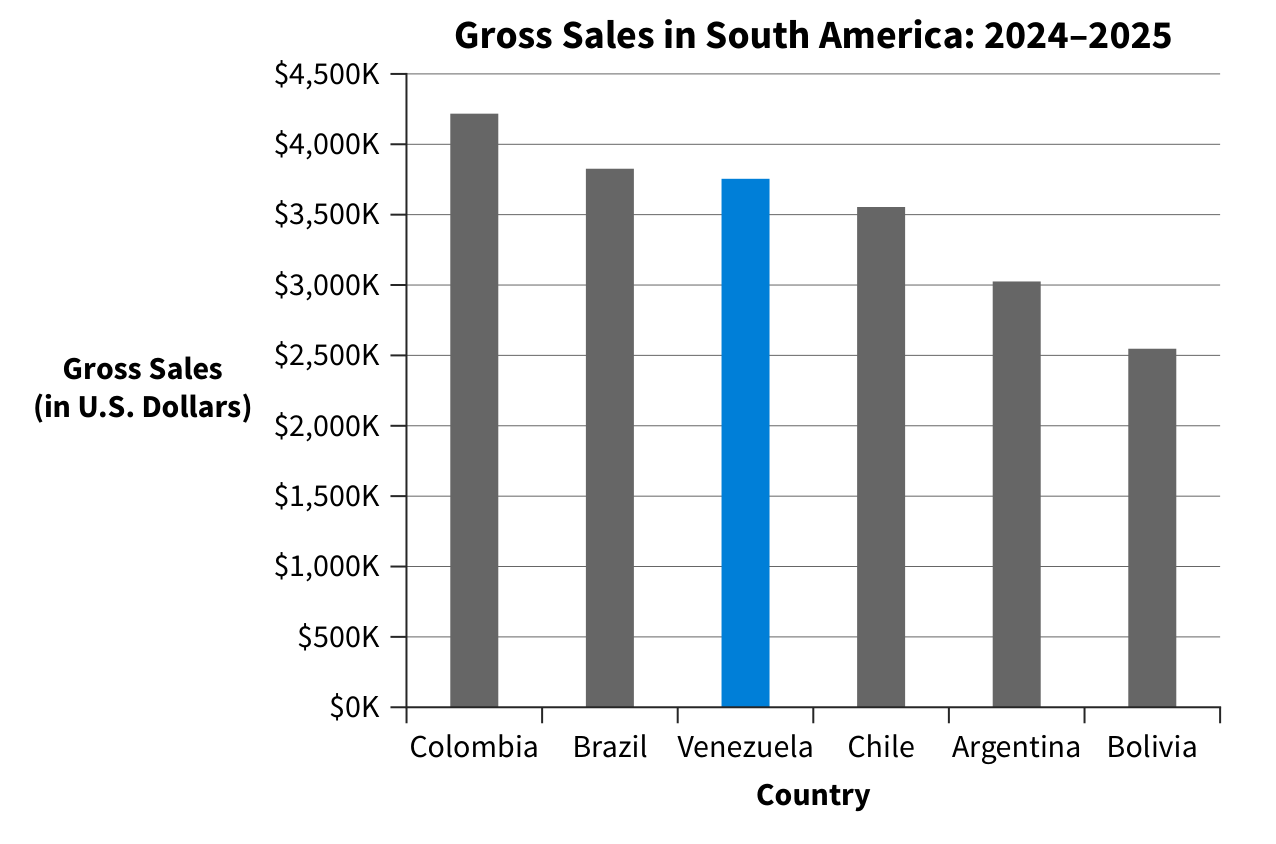
\includegraphics[width=0.95\textwidth,height=0.75\textheight,keepaspectratio]{../textbookForPractice/Figures/Ch_09/ILLUSTRATION 9.25.png}
    \end{figure}
\end{frame}

\begin{frame}{ILLUSTRATION 9.26}

    \begin{figure}[h]
        \centering
        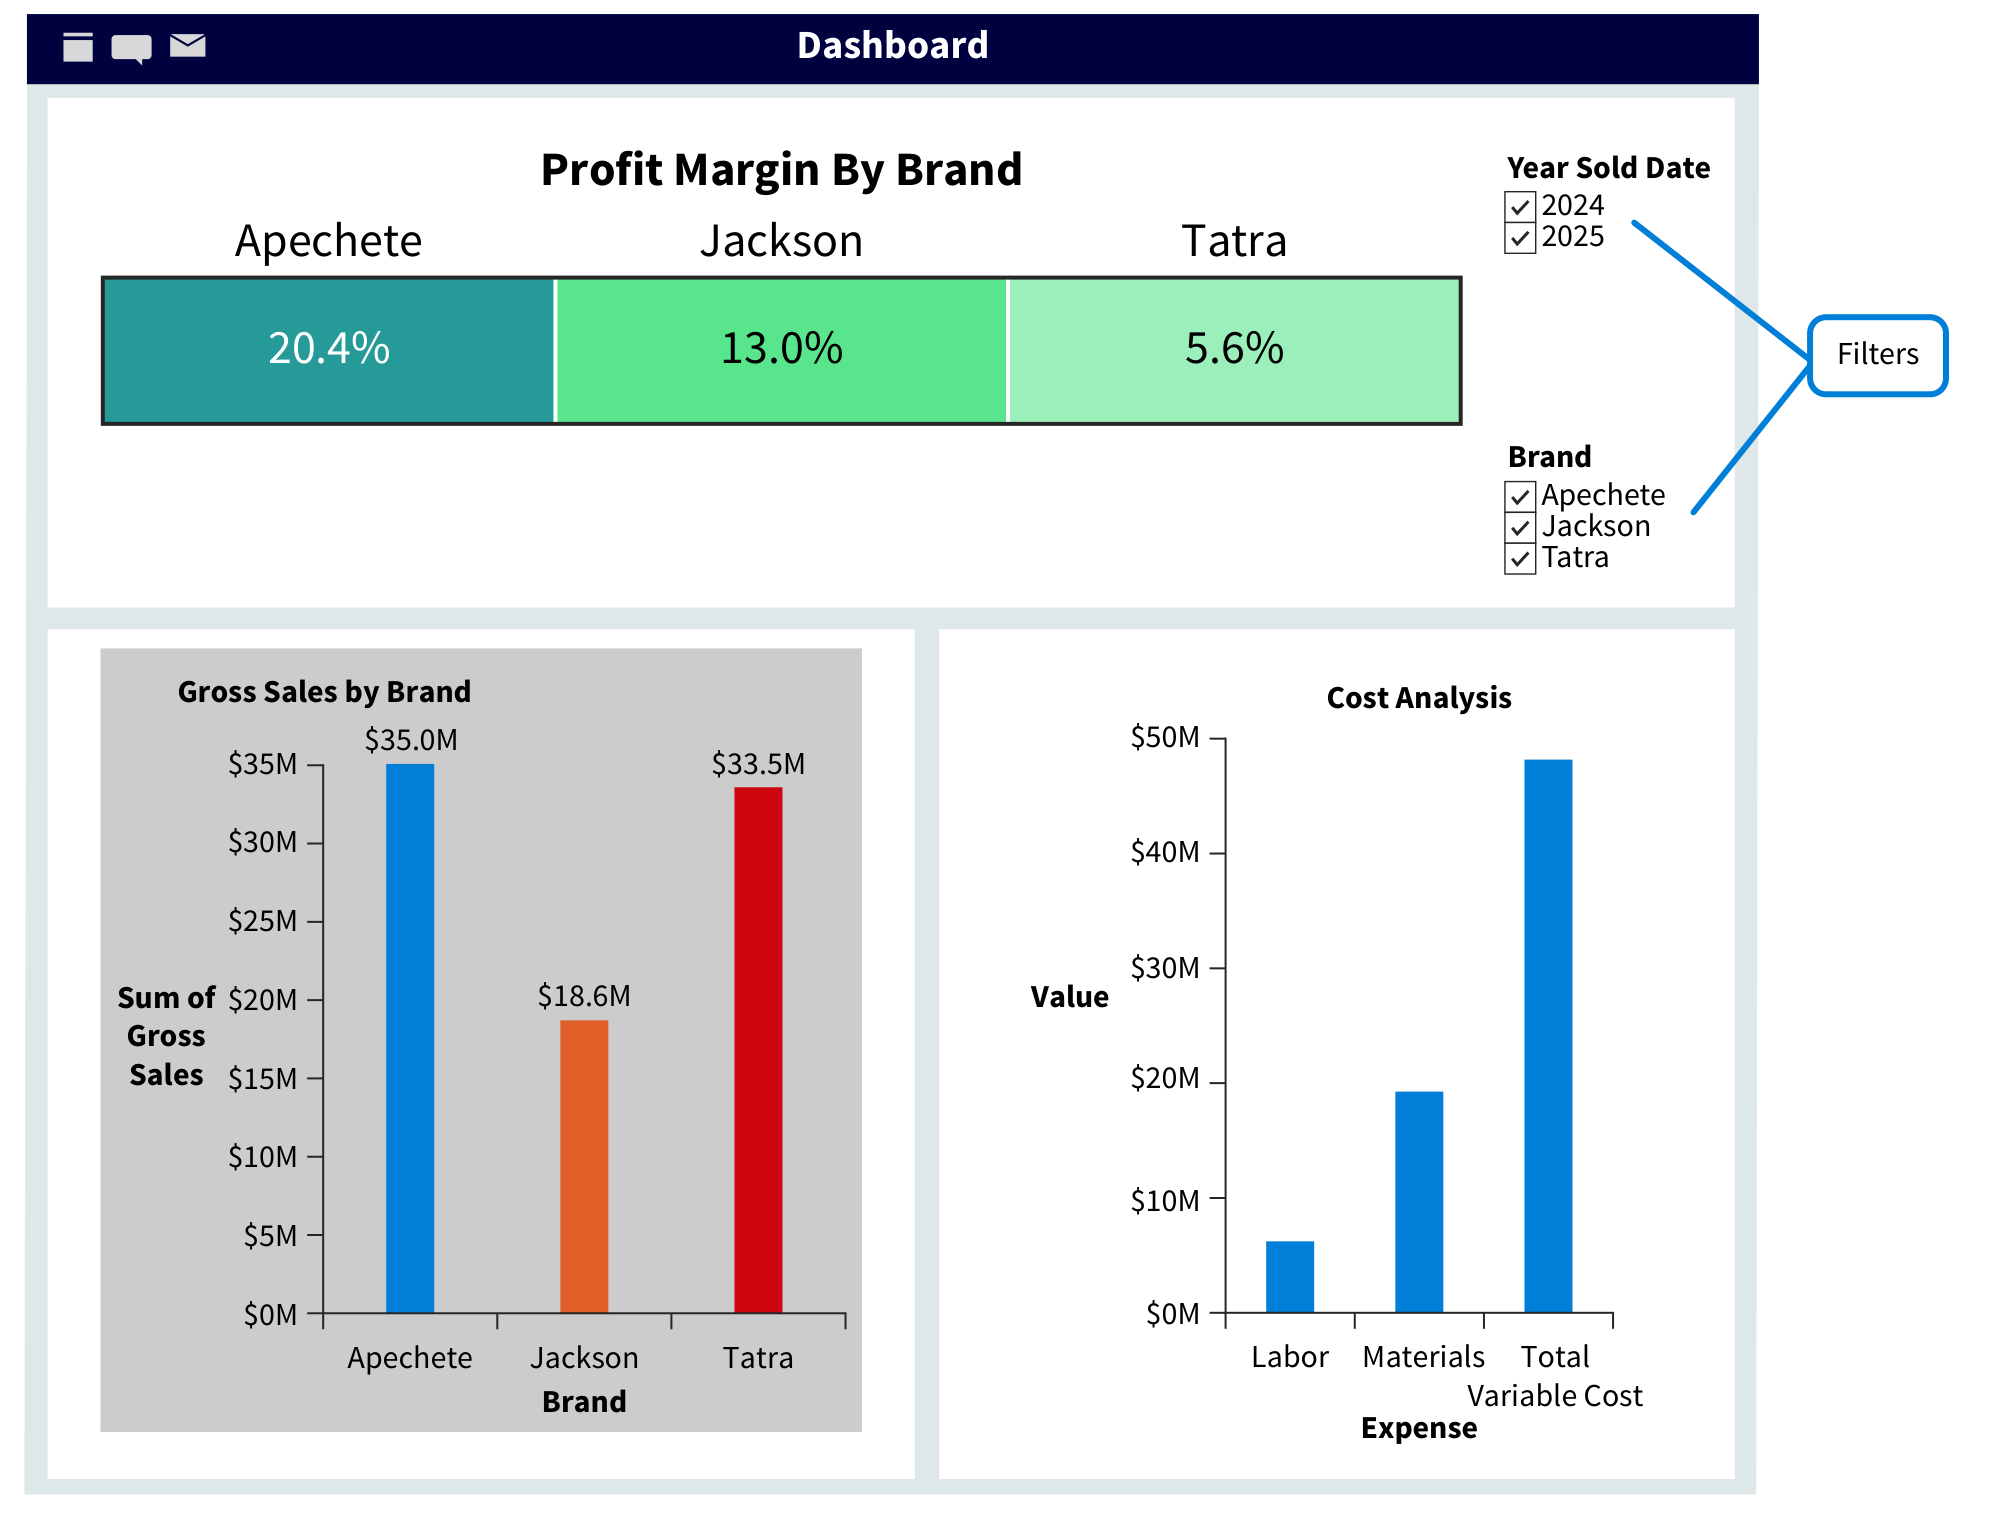
\includegraphics[width=0.95\textwidth,height=0.75\textheight,keepaspectratio]{../textbookForPractice/Figures/Ch_09/ILLUSTRATION 9.26.png}
    \end{figure}
\end{frame}

\begin{frame}{ILLUSTRATION 9.27}

    \begin{figure}[h]
        \centering
        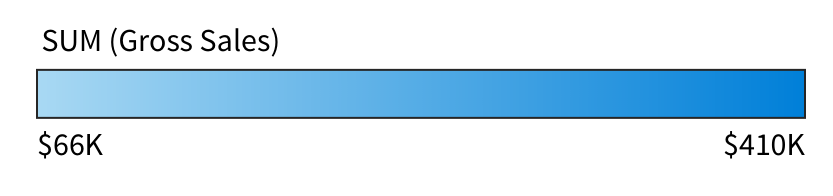
\includegraphics[width=0.95\textwidth,height=0.75\textheight,keepaspectratio]{../textbookForPractice/Figures/Ch_09/ILLUSTRATION 9.27.png}
    \end{figure}
\end{frame}

\begin{frame}{Các Thuộc tính Tiền-chú-ý (Preattentive Attributes)}
\begin{itemize}
    \item \textbf{Định nghĩa:} Các đặc điểm mà não bộ xử lý vô thức trước cả khi ta tập trung suy nghĩ.
    \item \textbf{Màu sắc (Color):} Sử dụng màu đỏ để nhấn mạnh sự bất thường hoặc thua lỗ.
    \item \textbf{Kích thước \& Hình dạng (Size \& Shape):} Dùng điểm lớn hơn hoặc đường nét đậm hơn để nhấn mạnh dữ liệu quan trọng nhất.
\end{itemize}
\end{frame}

\begin{frame}{ILLUSTRATION 9.28}

    \begin{figure}[h]
        \centering
        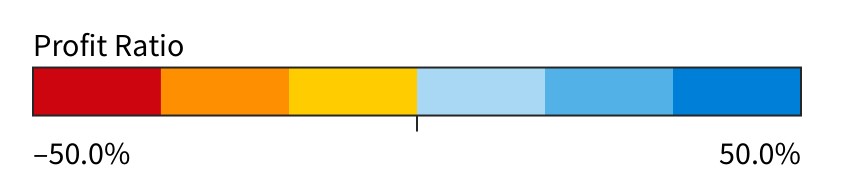
\includegraphics[width=0.95\textwidth,height=0.75\textheight,keepaspectratio]{../textbookForPractice/Figures/Ch_09/ILLUSTRATION 9.28.png}
    \end{figure}
\end{frame}

\begin{frame}{ILLUSTRATION 9.29}

    \begin{figure}[h]
        \centering
        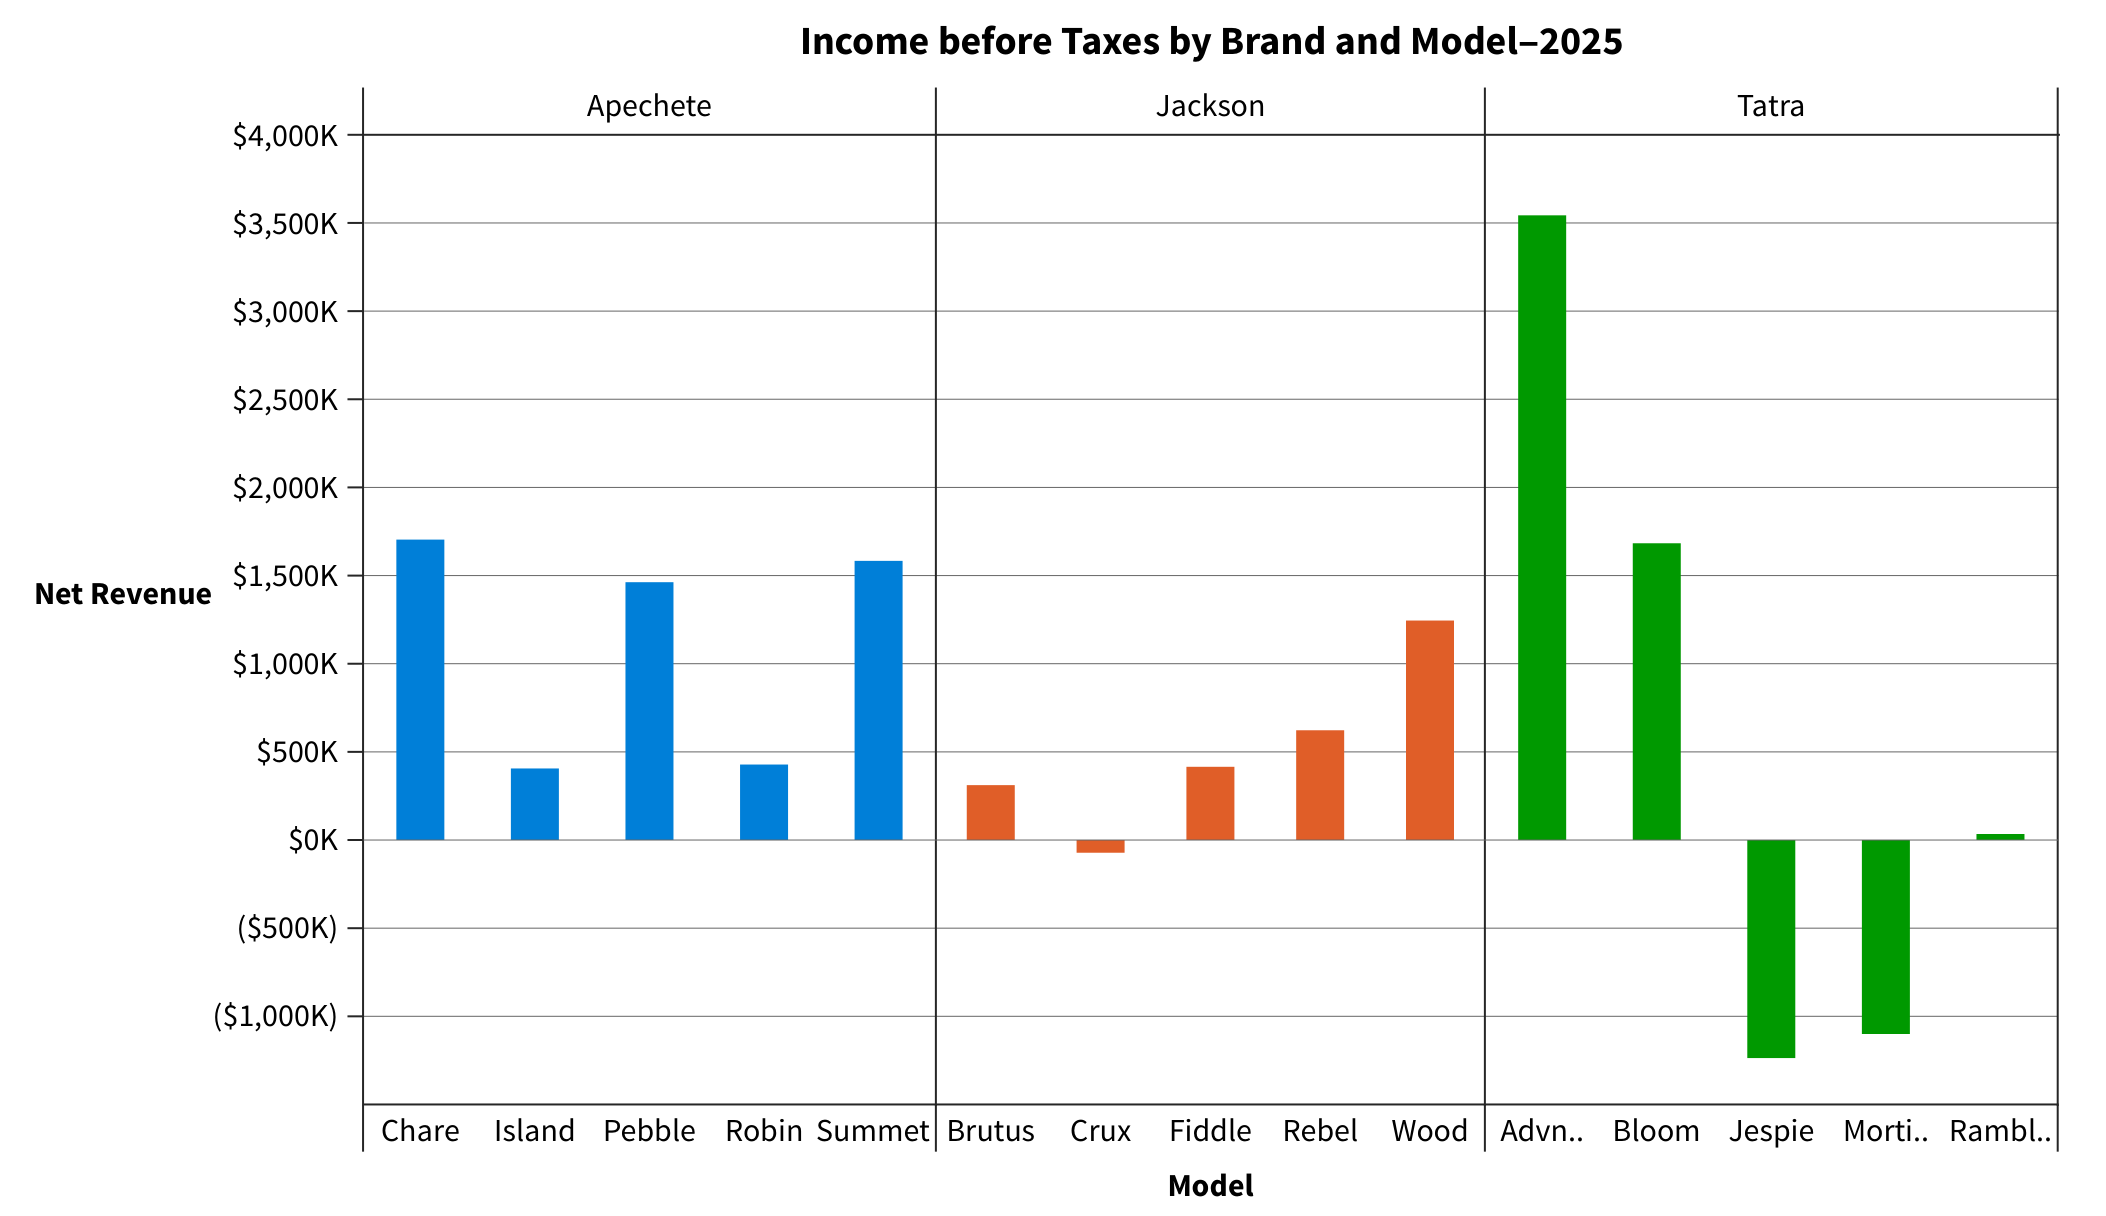
\includegraphics[width=0.95\textwidth,height=0.75\textheight,keepaspectratio]{../textbookForPractice/Figures/Ch_09/ILLUSTRATION 9.29.png}
    \end{figure}
\end{frame}

\begin{frame}{ILLUSTRATION 9.30}

    \begin{figure}[h]
        \centering
        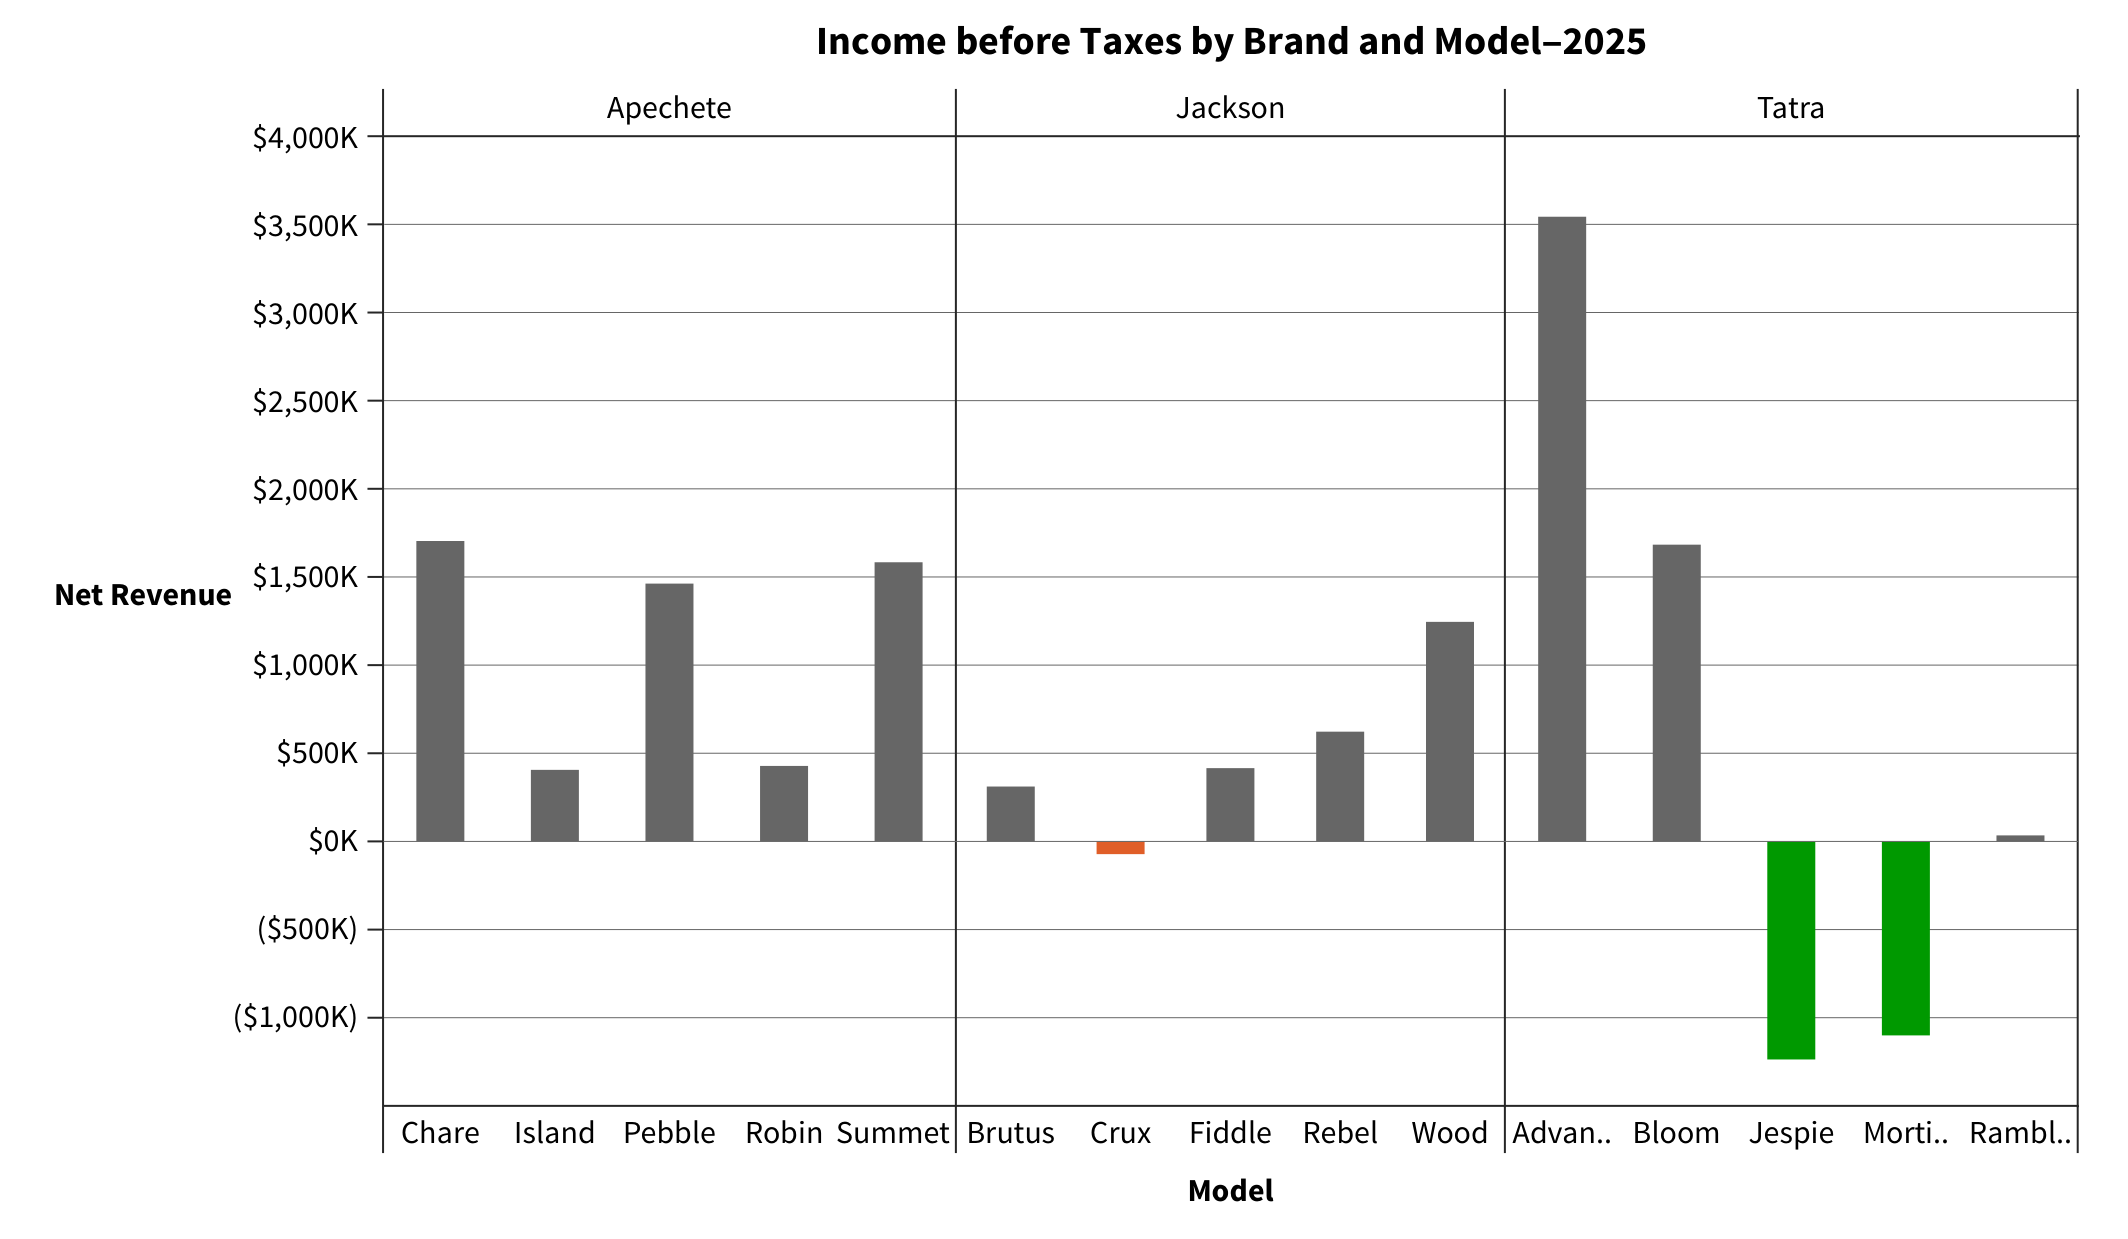
\includegraphics[width=0.95\textwidth,height=0.75\textheight,keepaspectratio]{../textbookForPractice/Figures/Ch_09/ILLUSTRATION 9.30.png}
    \end{figure}
\end{frame}

\begin{frame}{Tối Giản Hóa và Tránh Lộn Xộn}
\begin{itemize}
    \item \textbf{Avoid Clutter:} Tránh sự rối rắm không cần thiết.
    \item \textbf{Chartjunk:} Các thành phần trang trí không mang lại giá trị thông tin (VD: Hiệu ứng 3D, lưới nền quá đậm, màu sắc sặc sỡ không cần thiết).
    \item Tối giản hóa giúp thông điệp chính nổi bật (Nguyên lý Tỷ lệ Dữ liệu/Mực in - Data-ink ratio).
\end{itemize}
\end{frame}

\begin{frame}{ILLUSTRATION 9.31}

    \begin{figure}[h]
        \centering
        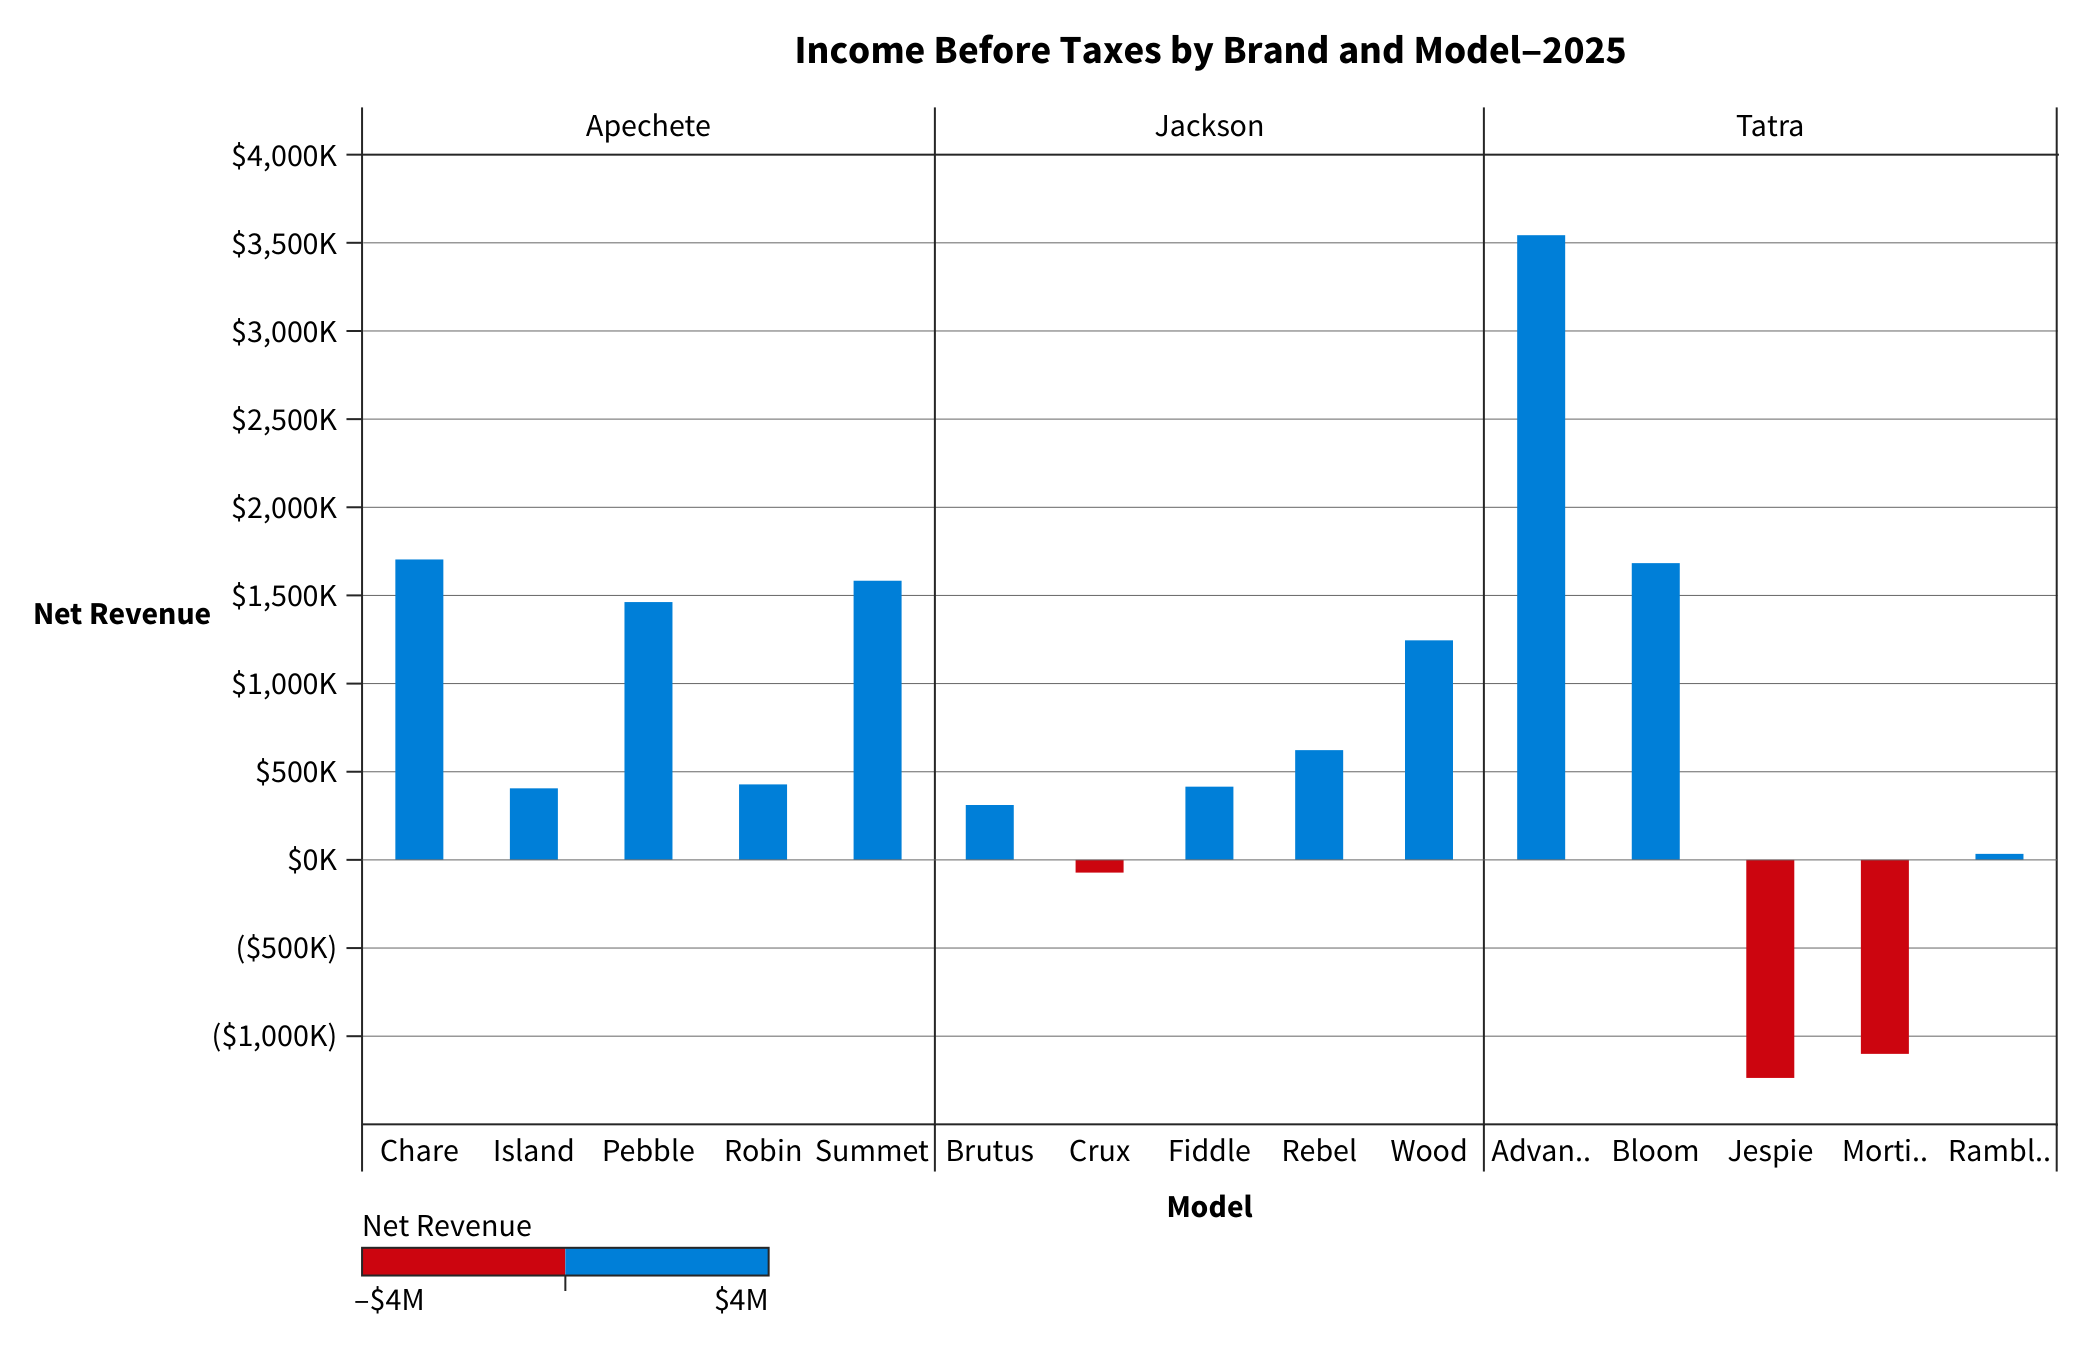
\includegraphics[width=0.95\textwidth,height=0.75\textheight,keepaspectratio]{../textbookForPractice/Figures/Ch_09/ILLUSTRATION 9.31.png}
    \end{figure}
\end{frame}

\begin{frame}{ILLUSTRATION 9.32}

    \begin{figure}[h]
        \centering
        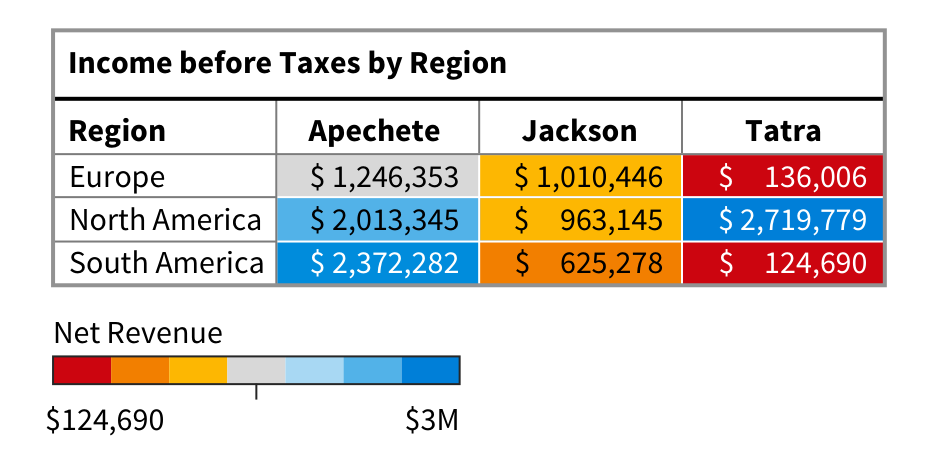
\includegraphics[width=0.95\textwidth,height=0.75\textheight,keepaspectratio]{../textbookForPractice/Figures/Ch_09/ILLUSTRATION 9.32.png}
    \end{figure}
\end{frame}

\begin{frame}{ILLUSTRATION 9.33}

    \begin{figure}[h]
        \centering
        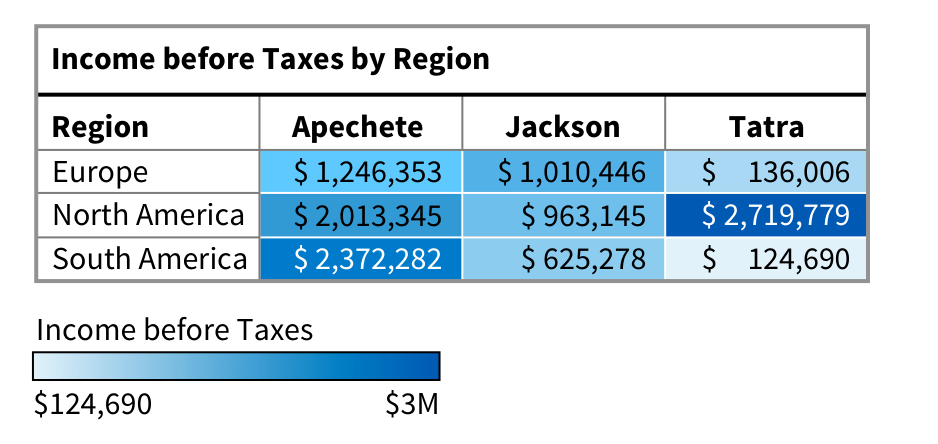
\includegraphics[width=0.95\textwidth,height=0.75\textheight,keepaspectratio]{../textbookForPractice/Figures/Ch_09/ILLUSTRATION 9.33.png}
    \end{figure}
\end{frame}

\begin{frame}{9.4 Nhận Diện Trực Quan Hóa Gây Hiểu Lầm}
\begin{itemize}
    \item Dữ liệu có thể không biết nói dối, nhưng biểu đồ thì có thể (Misleading Data Visualizations).
    \item Việc thiết kế sai nguyên tắc có thể bóp méo góc nhìn của người xem.
    \item Kế toán viên cần tinh ý nhận diện những cạm bẫy thiết kế phổ biến.
\end{itemize}
\end{frame}

\begin{frame}{ILLUSTRATION 9.34}

    \begin{figure}[h]
        \centering
        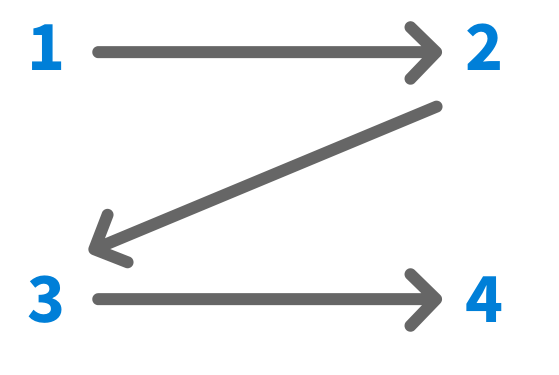
\includegraphics[width=0.95\textwidth,height=0.75\textheight,keepaspectratio]{../textbookForPractice/Figures/Ch_09/ILLUSTRATION 9.34.png}
    \end{figure}
\end{frame}

\begin{frame}{ILLUSTRATION 9.35}

    \begin{figure}[h]
        \centering
        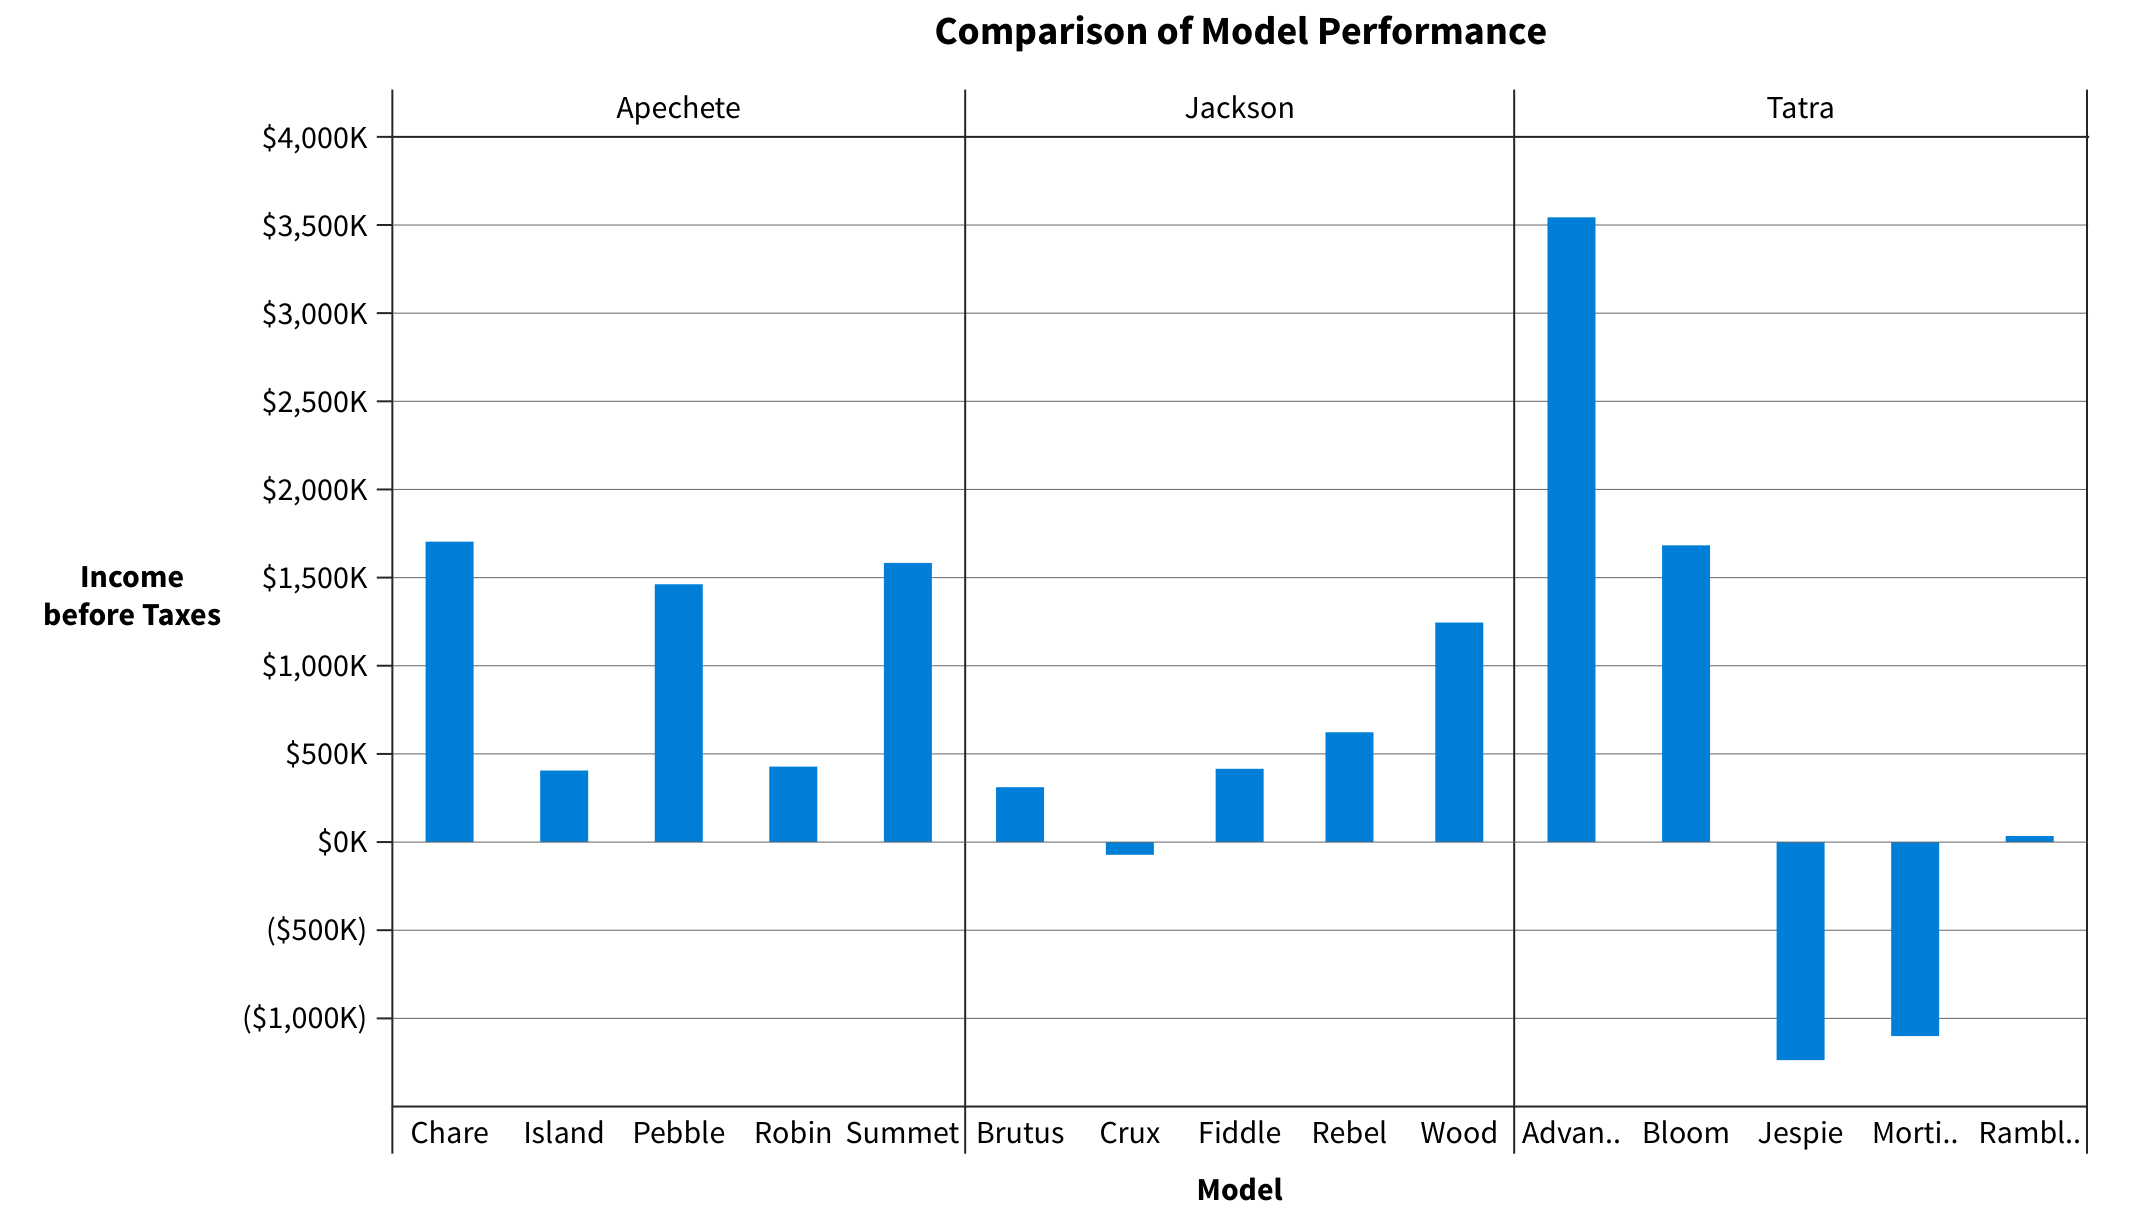
\includegraphics[width=0.95\textwidth,height=0.75\textheight,keepaspectratio]{../textbookForPractice/Figures/Ch_09/ILLUSTRATION 9.35.png}
    \end{figure}
\end{frame}

\begin{frame}{ILLUSTRATION 9.36}

    \begin{figure}[h]
        \centering
        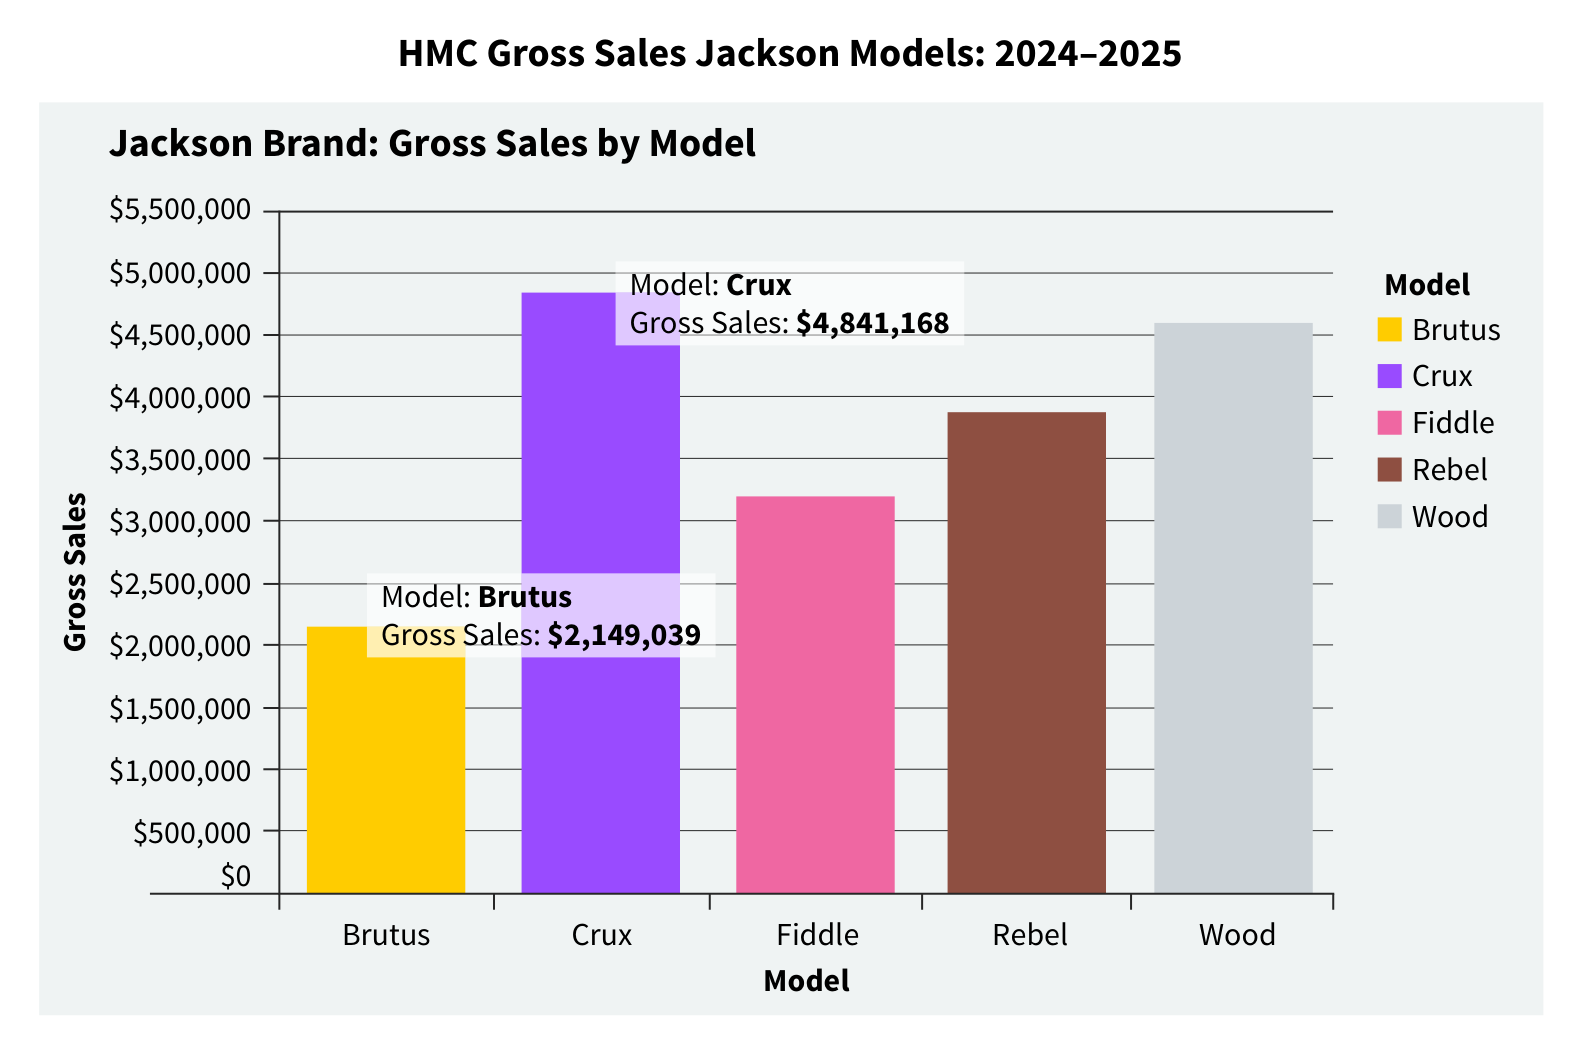
\includegraphics[width=0.95\textwidth,height=0.75\textheight,keepaspectratio]{../textbookForPractice/Figures/Ch_09/ILLUSTRATION 9.36.png}
    \end{figure}
\end{frame}

\begin{frame}{Lỗi 1: Bỏ qua đường cơ sở (Omitting Baseline)}
\begin{itemize}
    \item Đối với biểu đồ cột (Bar chart), trục Y \textbf{bắt buộc} phải bắt đầu từ số 0.
    \item \textbf{Hậu quả:} Nếu trục Y bị cắt xén, một sự chênh lệch nhỏ sẽ bị khuếch đại thành một sự thay đổi khổng lồ.
\end{itemize}
\end{frame}

\begin{frame}{ILLUSTRATION 9.37}

    \begin{figure}[h]
        \centering
        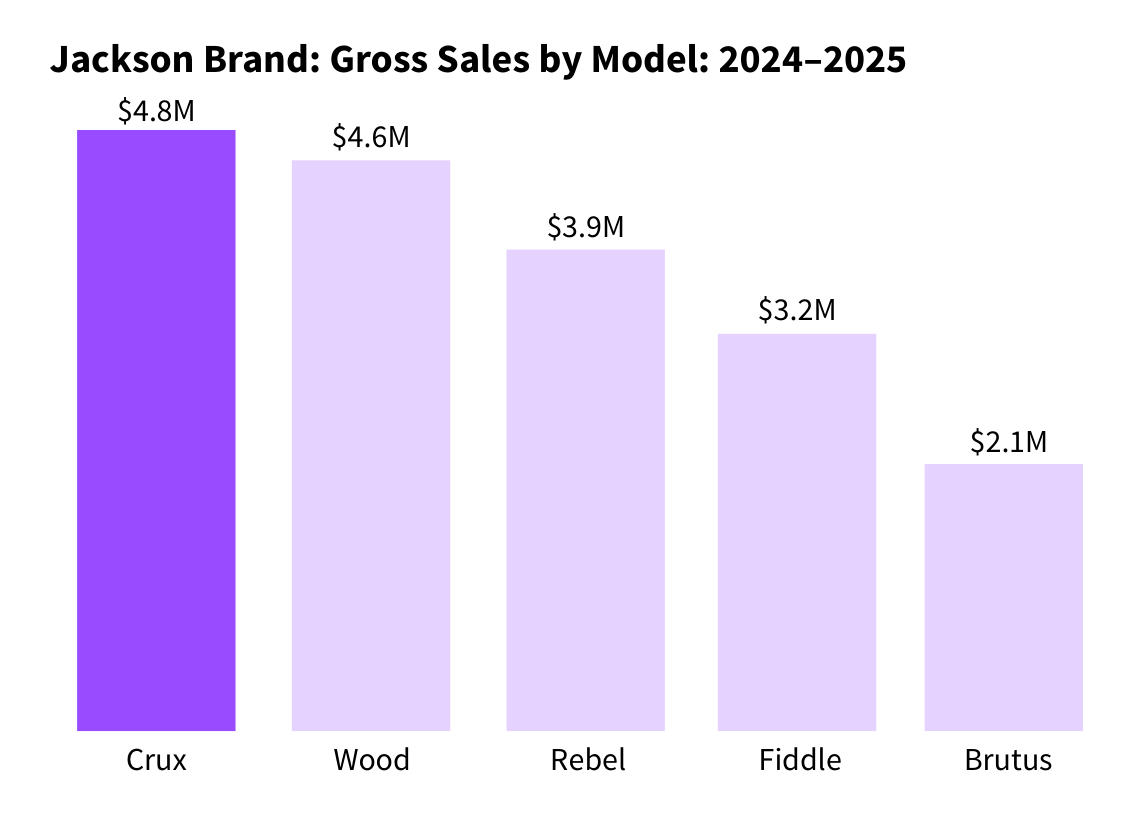
\includegraphics[width=0.95\textwidth,height=0.75\textheight,keepaspectratio]{../textbookForPractice/Figures/Ch_09/ILLUSTRATION 9.37.png}
    \end{figure}
\end{frame}

\begin{frame}{ILLUSTRATION 9.38}

    \begin{figure}[h]
        \centering
        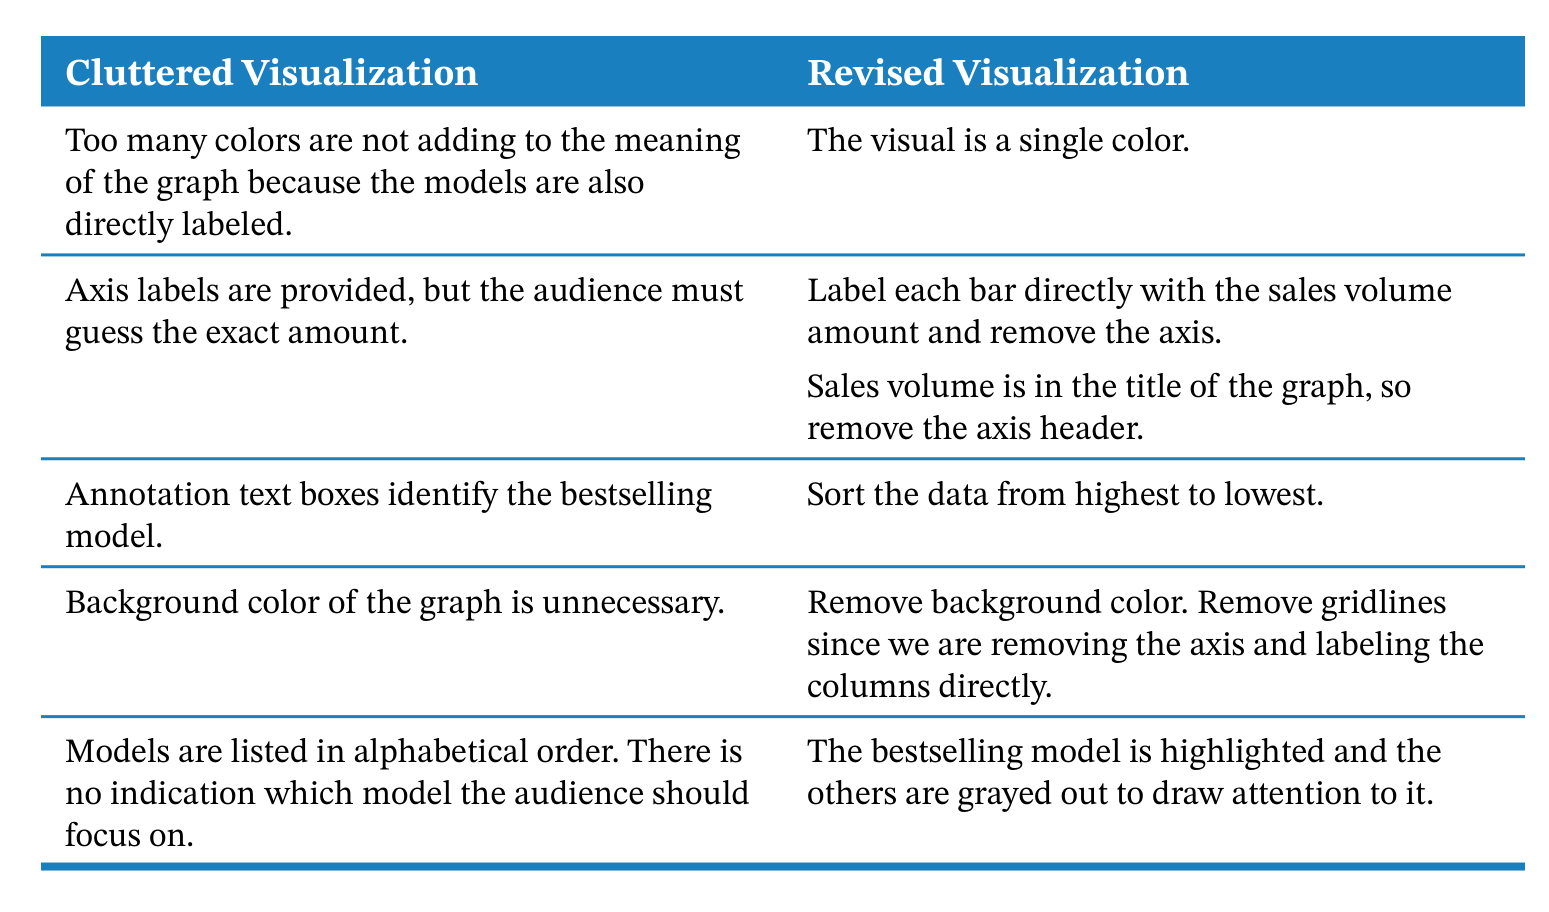
\includegraphics[width=0.95\textwidth,height=0.75\textheight,keepaspectratio]{../textbookForPractice/Figures/Ch_09/ILLUSTRATION 9.38.png}
    \end{figure}
\end{frame}

\begin{frame}{ILLUSTRATION 9.39}

    \begin{figure}[h]
        \centering
        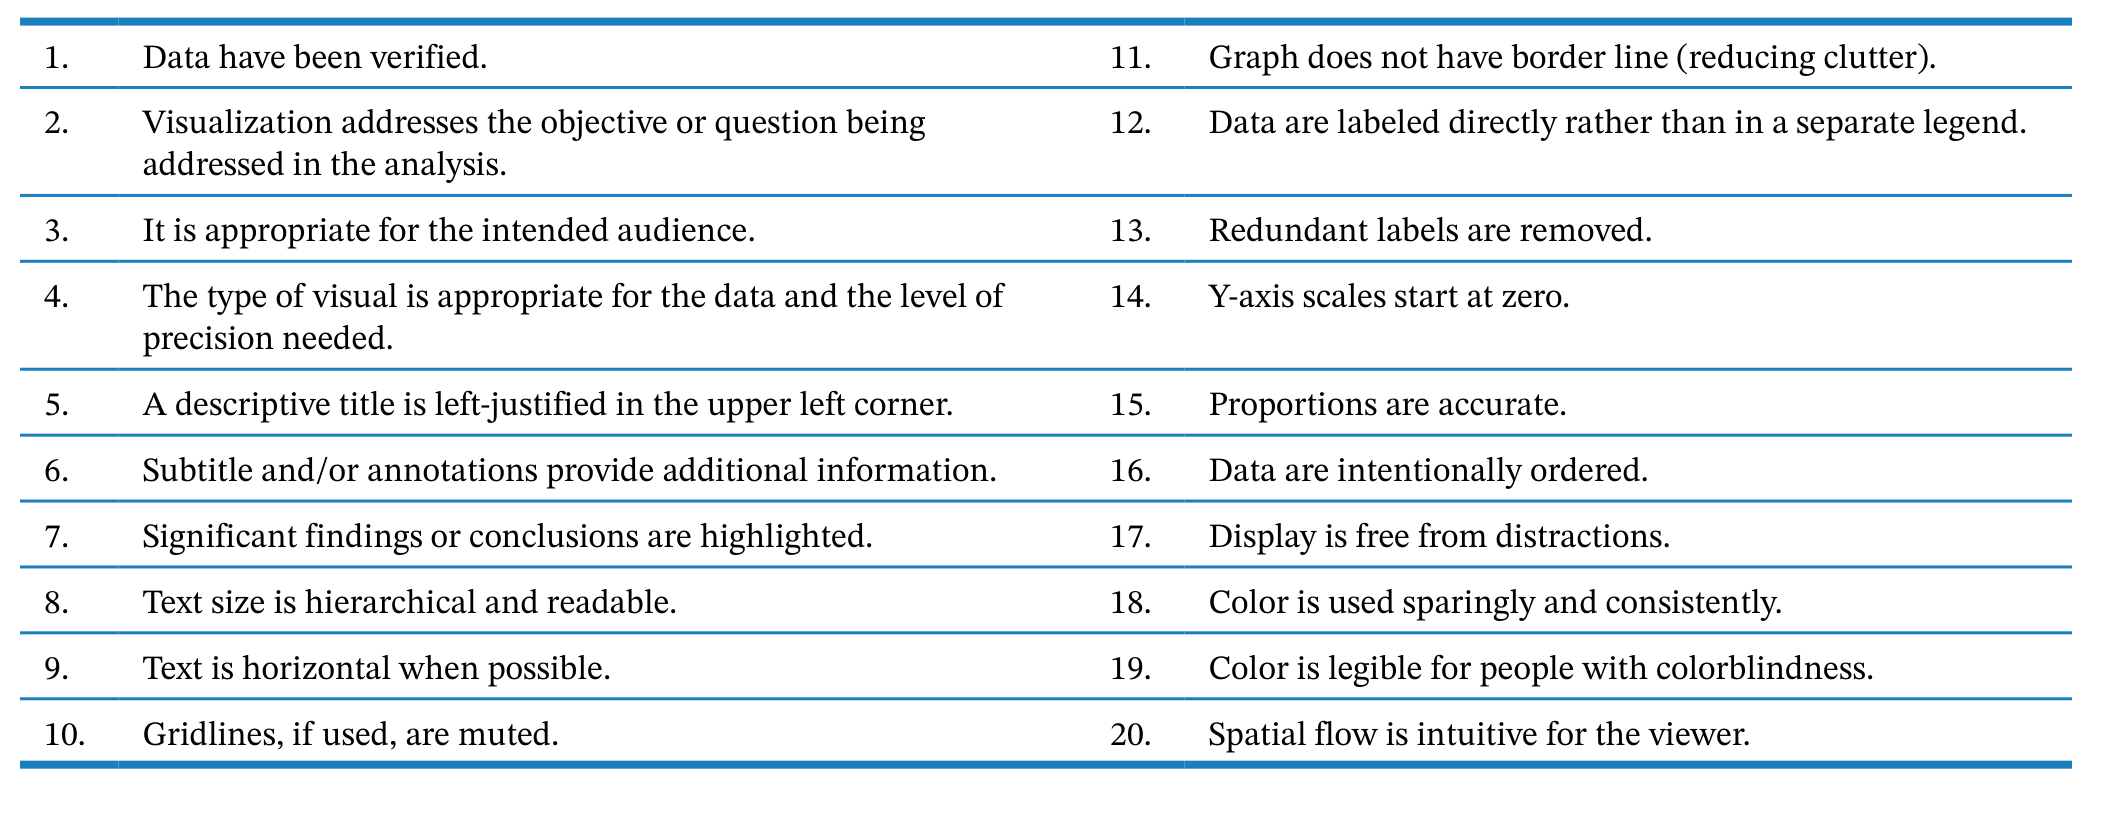
\includegraphics[width=0.95\textwidth,height=0.75\textheight,keepaspectratio]{../textbookForPractice/Figures/Ch_09/ILLUSTRATION 9.39.png}
    \end{figure}
\end{frame}

\begin{frame}{Lỗi 2: Thao Túng Trục Y}
\begin{itemize}
    \item \textbf{Đảo ngược trục (Inverted Y-axis):} Gây cảm giác lầm tưởng rằng số liệu đang tăng trong khi thực tế đang giảm.
    \item \textbf{Chia tỷ lệ không đều (Uneven scaling):} Trục tọa độ giãn cách không đều làm đường xu hướng bị biến dạng.
\end{itemize}
\end{frame}

\begin{frame}{ILLUSTRATION 9.40A}

    \begin{figure}[h]
        \centering
        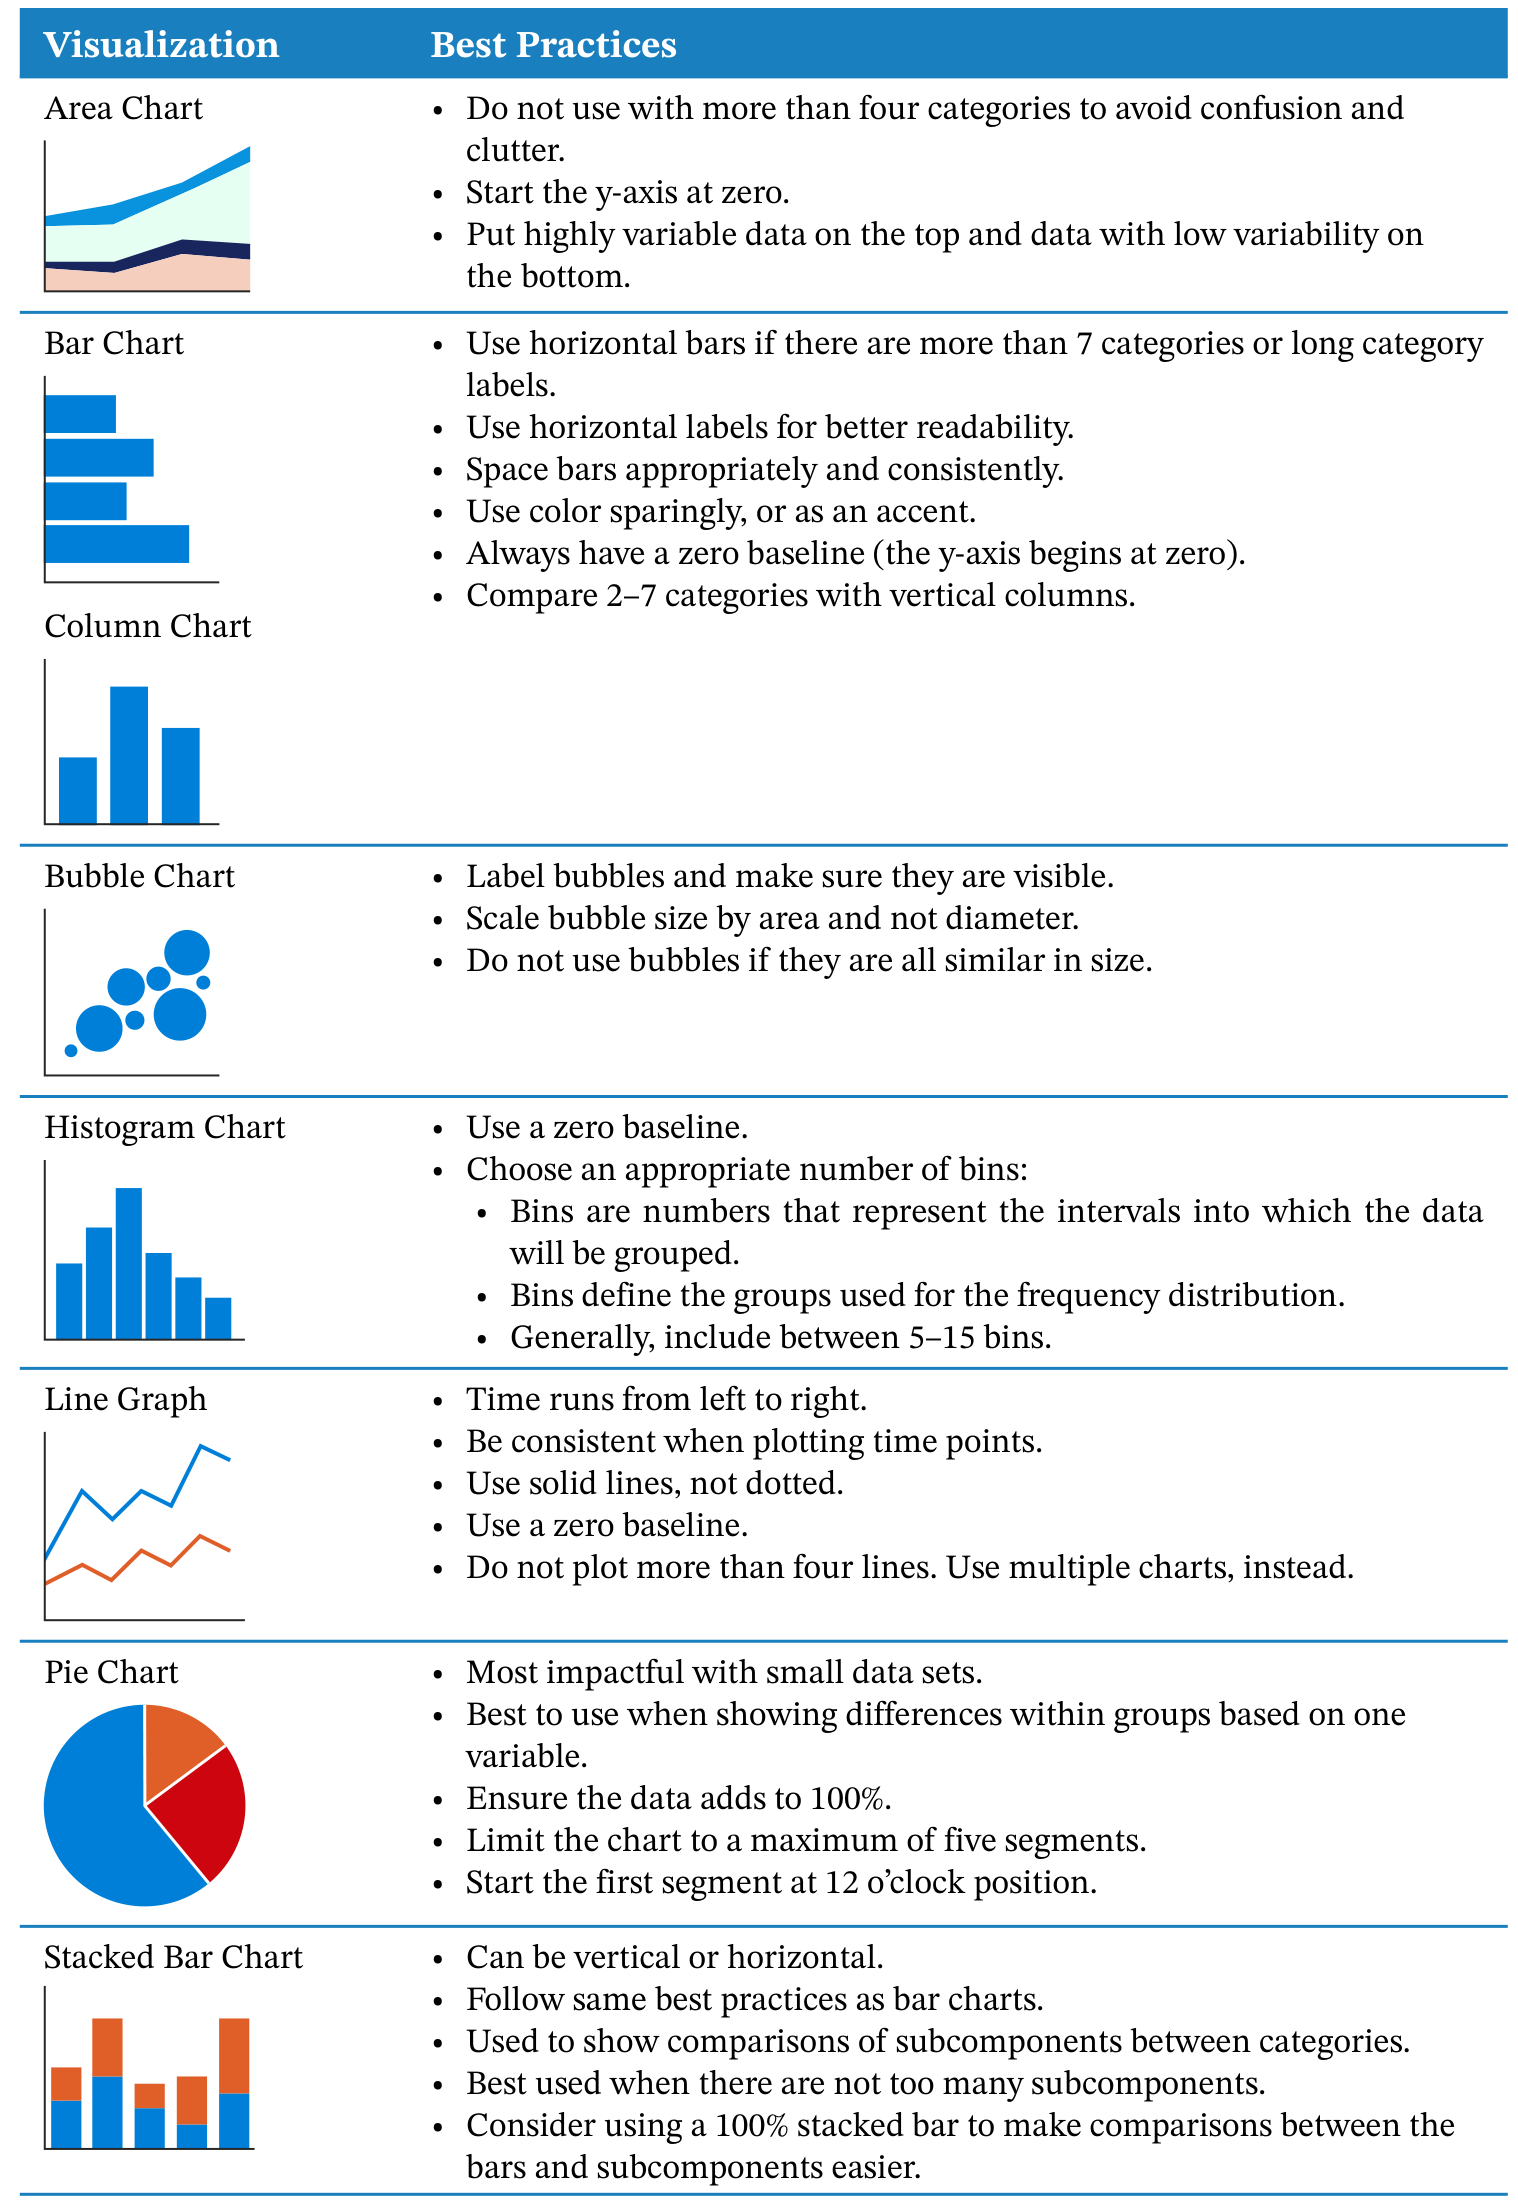
\includegraphics[width=0.95\textwidth,height=0.75\textheight,keepaspectratio]{../textbookForPractice/Figures/Ch_09/ILLUSTRATION 9.40A.png}
    \end{figure}
\end{frame}

\begin{frame}{ILLUSTRATION 9.40B}

    \begin{figure}[h]
        \centering
        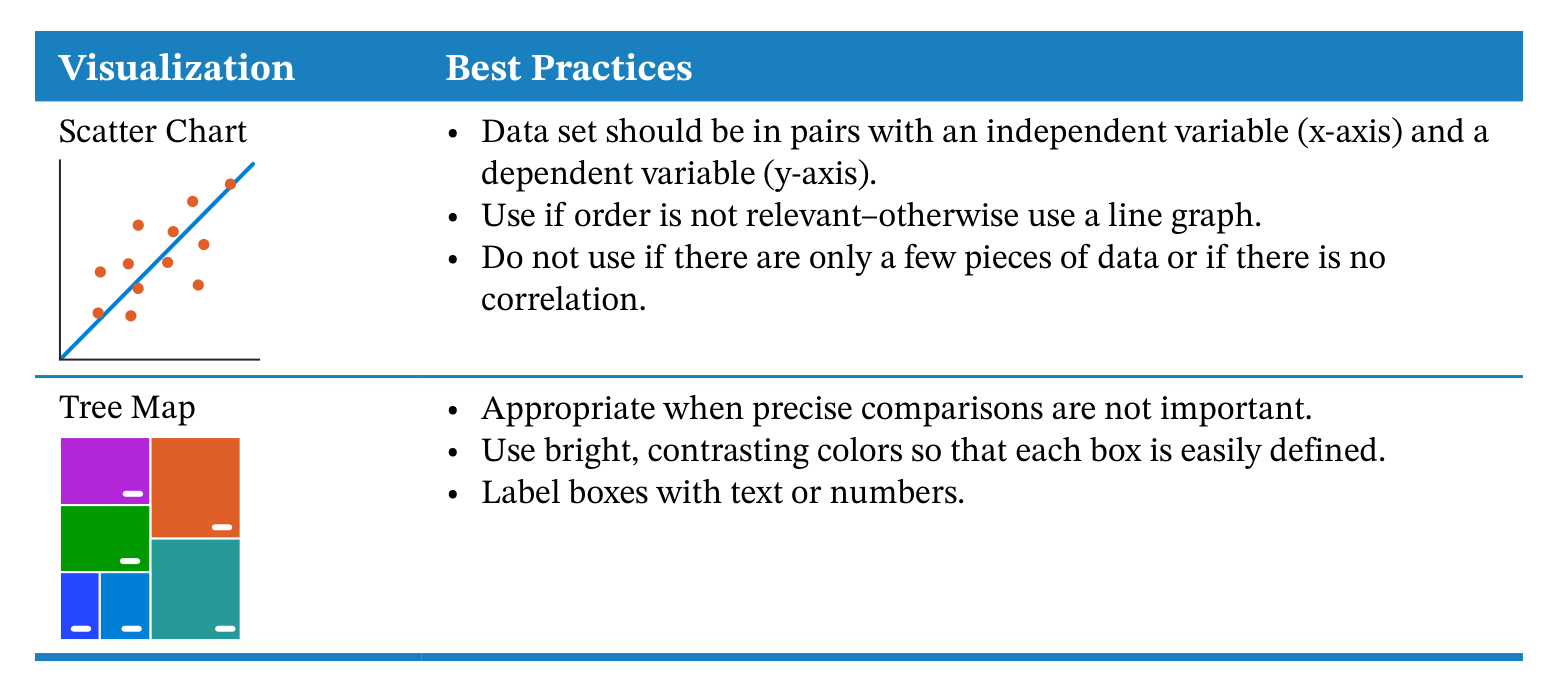
\includegraphics[width=0.95\textwidth,height=0.75\textheight,keepaspectratio]{../textbookForPractice/Figures/Ch_09/ILLUSTRATION 9.40B.png}
    \end{figure}
\end{frame}

\begin{frame}{ILLUSTRATION 9.41}

    \begin{figure}[h]
        \centering
        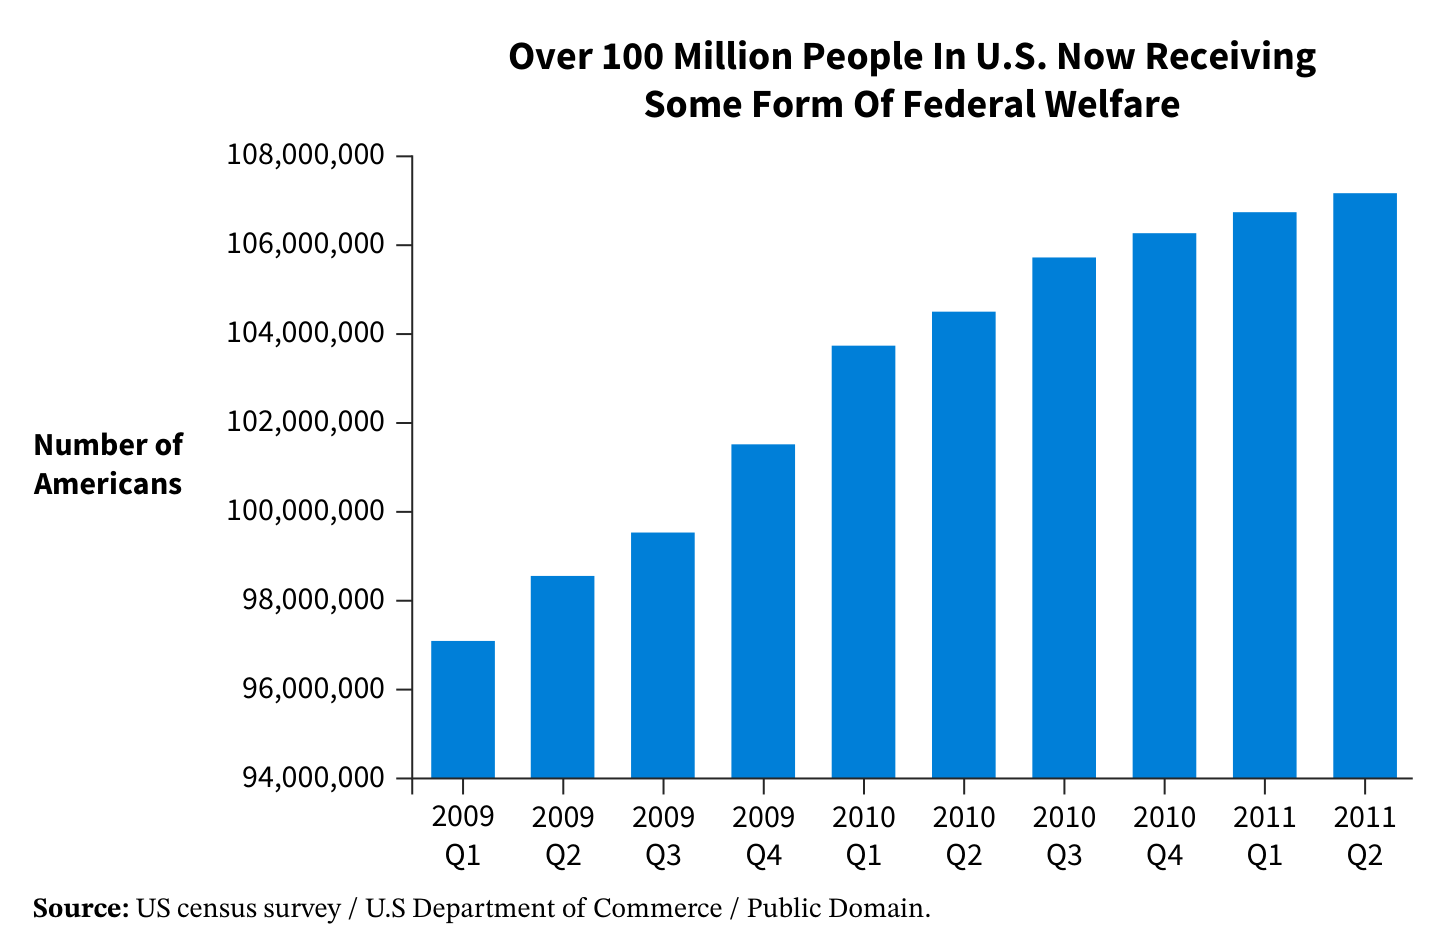
\includegraphics[width=0.95\textwidth,height=0.75\textheight,keepaspectratio]{../textbookForPractice/Figures/Ch_09/ILLUSTRATION 9.41.png}
    \end{figure}
\end{frame}

\begin{frame}{Lỗi 3: Đi Ngược Quy Ước Thiết Kế}
\begin{itemize}
    \item \textbf{Going Against Conventions:} Con người có các quy ước ngầm về màu sắc và không gian.
    \item \textit{Ví dụ:} Màu Đỏ thường mang ý nghĩa tiêu cực/lỗ, màu Xanh mang ý nghĩa tích cực/lãi. Dùng ngược lại sẽ gây nhầm lẫn trầm trọng.
    \item Trên/Phải thường mang ý nghĩa cao hơn/tăng lên. Dưới/Trái là giảm.
\end{itemize}
\end{frame}

\begin{frame}{ILLUSTRATION 9.42}

    \begin{figure}[h]
        \centering
        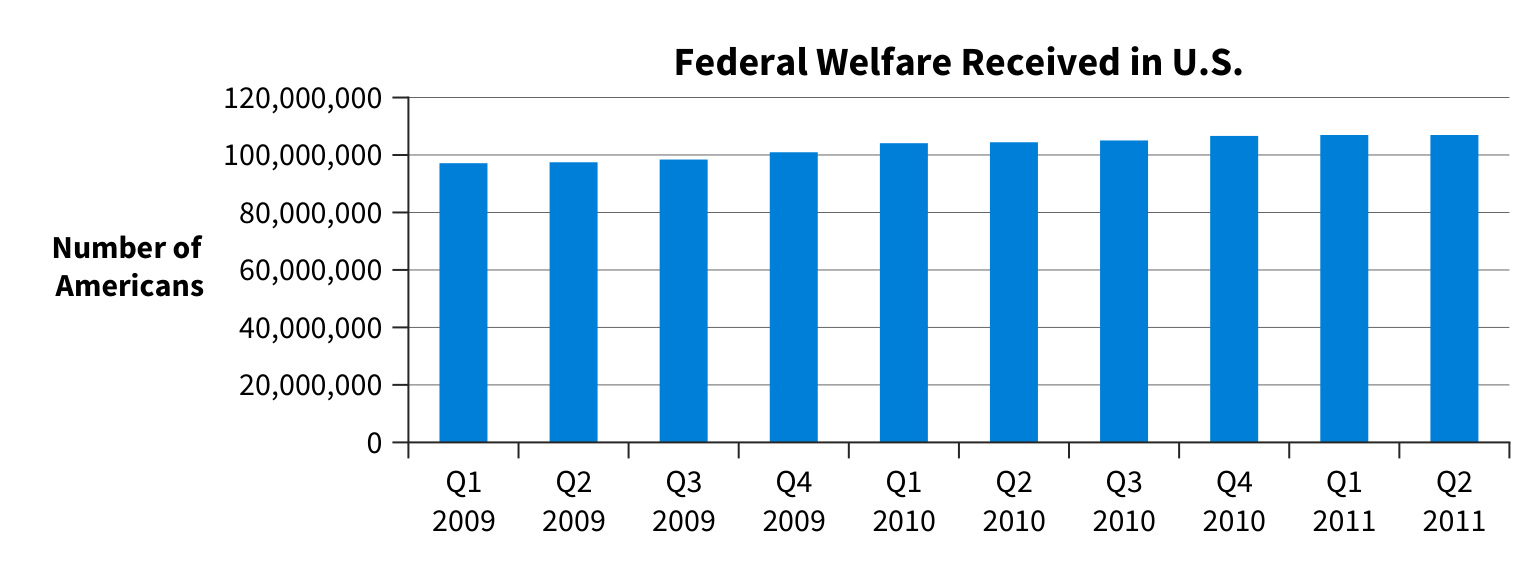
\includegraphics[width=0.95\textwidth,height=0.75\textheight,keepaspectratio]{../textbookForPractice/Figures/Ch_09/ILLUSTRATION 9.42.png}
    \end{figure}
\end{frame}

\begin{frame}{ILLUSTRATION 9.43}

    \begin{figure}[h]
        \centering
        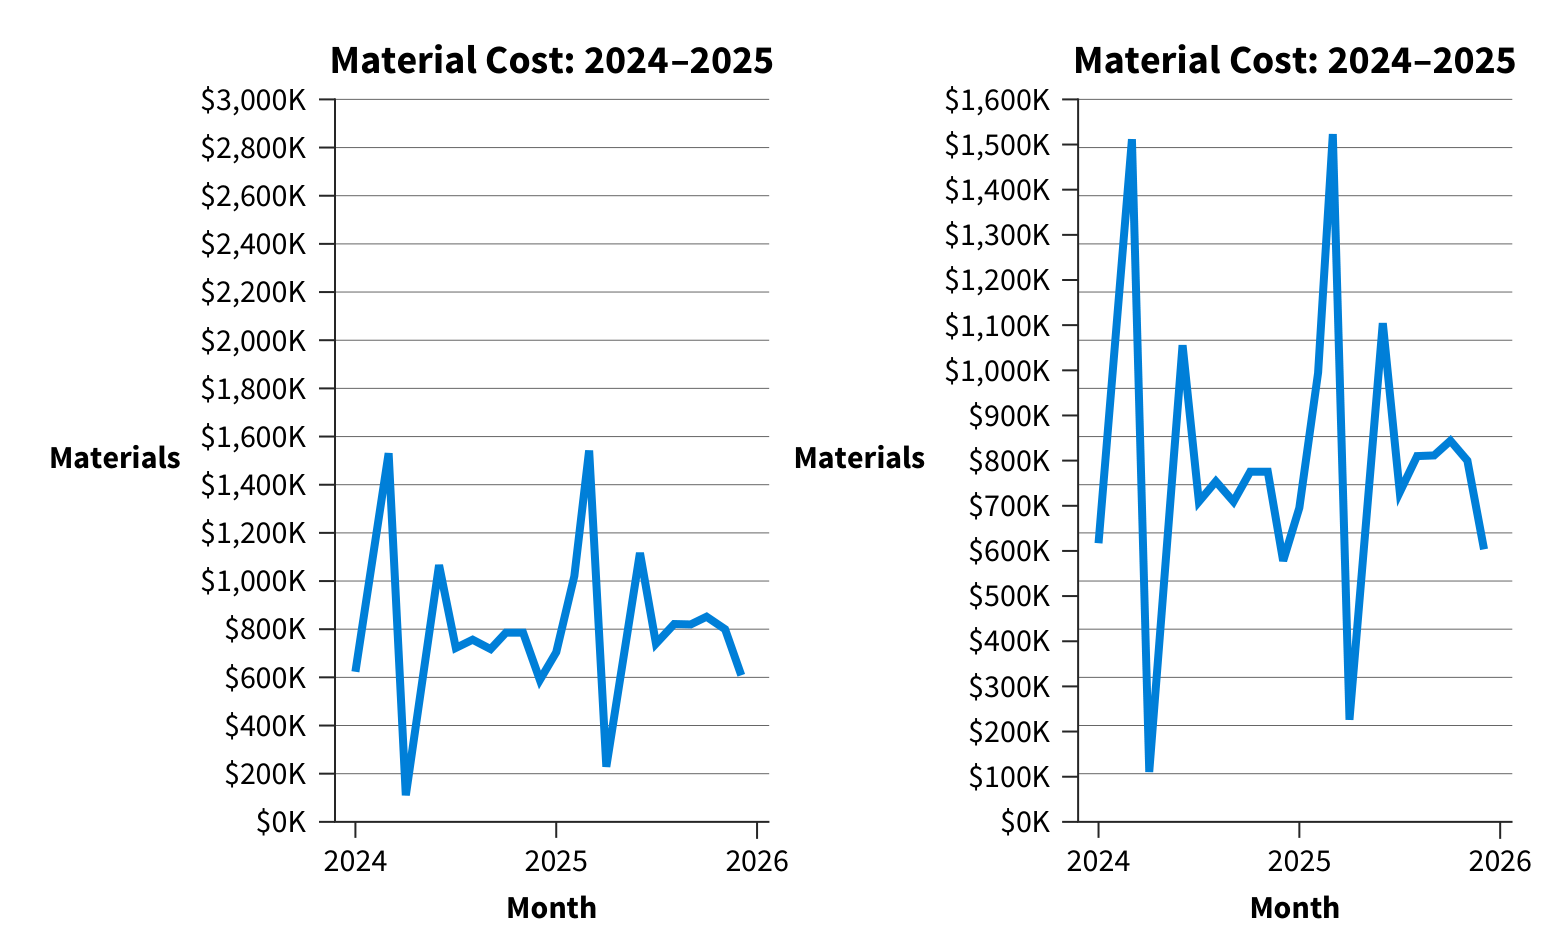
\includegraphics[width=0.95\textwidth,height=0.75\textheight,keepaspectratio]{../textbookForPractice/Figures/Ch_09/ILLUSTRATION 9.43.png}
    \end{figure}
\end{frame}

\begin{frame}{ILLUSTRATION 9.44}

    \begin{figure}[h]
        \centering
        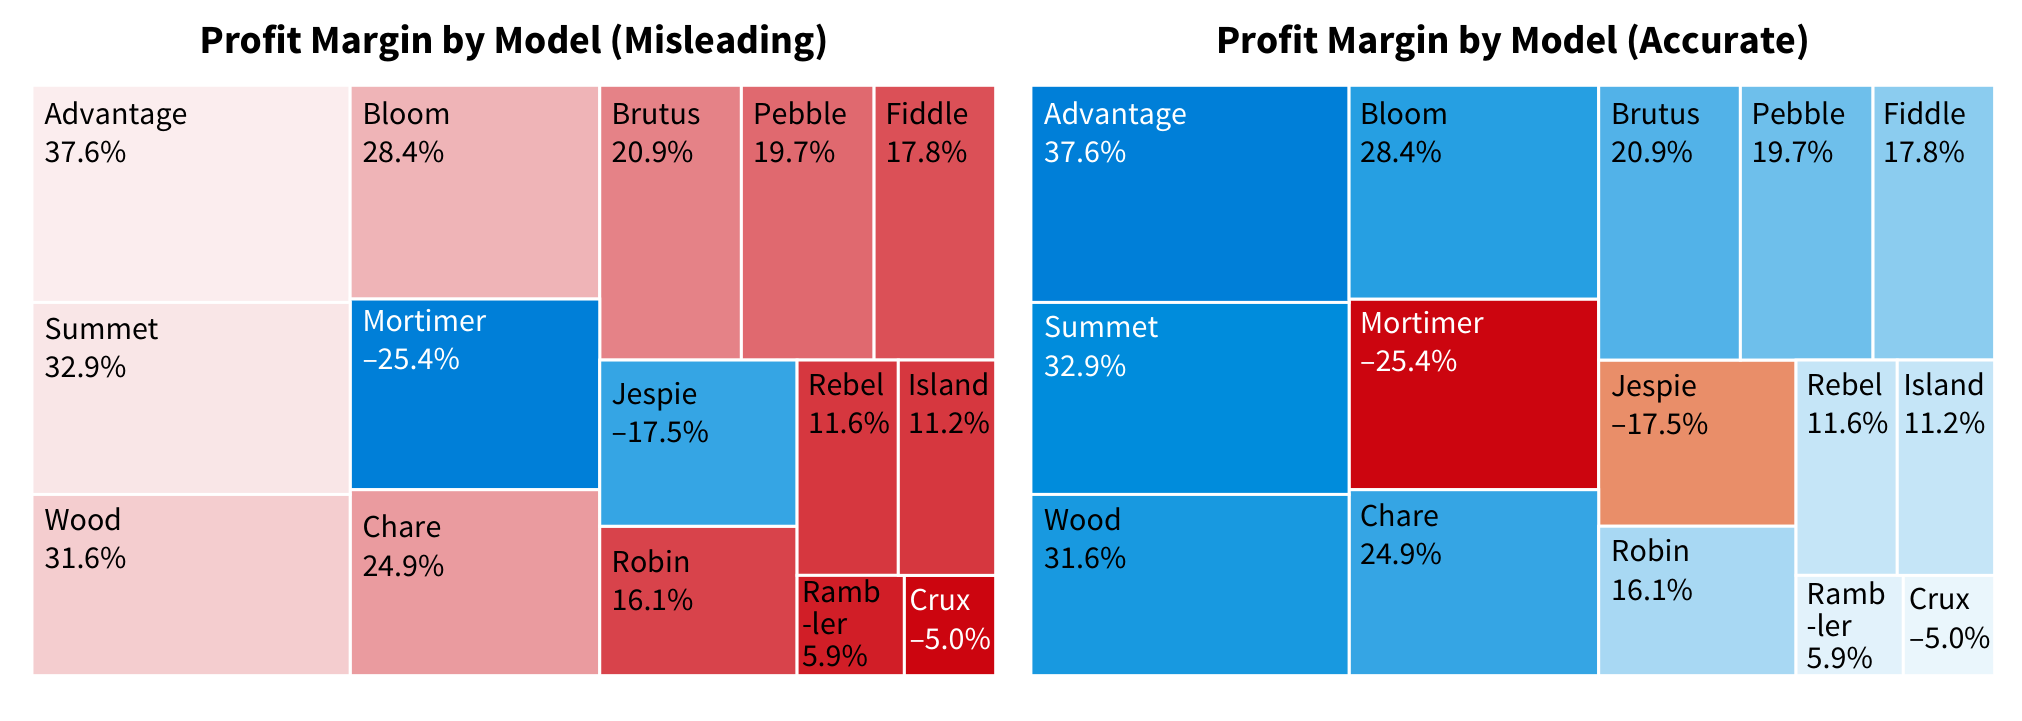
\includegraphics[width=0.95\textwidth,height=0.75\textheight,keepaspectratio]{../textbookForPractice/Figures/Ch_09/ILLUSTRATION 9.44.png}
    \end{figure}
\end{frame}

\begin{frame}{Lỗi 4: Chọn Lọc Dữ Liệu \& Dùng Sai Biểu Đồ}
\begin{itemize}
    \item \textbf{Cherry-picking:} Chỉ chọn hiển thị khoảng thời gian dữ liệu có lợi để che giấu bức tranh tổng thể.
    \item \textbf{Wrong Graph:} Dùng sai biểu đồ, ví dụ dùng Pie Chart (Biểu đồ tròn) cho dữ liệu tổng không bằng 100\%, hoặc dùng quá nhiều lát cắt.
\end{itemize}
\end{frame}

\begin{frame}{ILLUSTRATION 9.45}

    \begin{figure}[h]
        \centering
        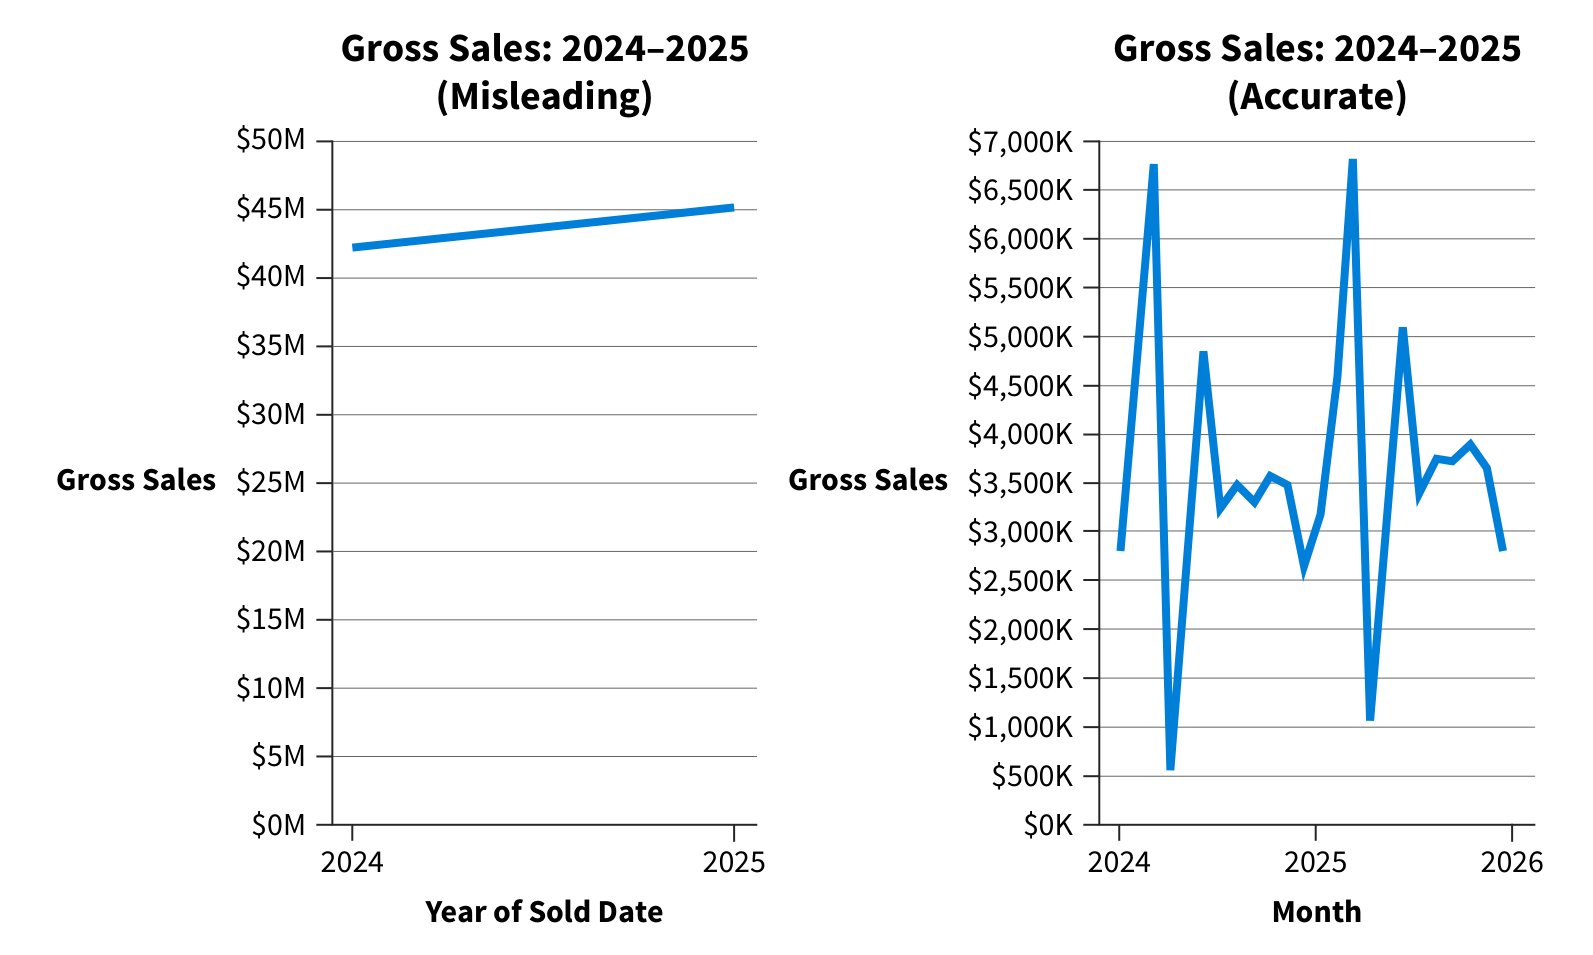
\includegraphics[width=0.95\textwidth,height=0.75\textheight,keepaspectratio]{../textbookForPractice/Figures/Ch_09/ILLUSTRATION 9.45.png}
    \end{figure}
\end{frame}

\begin{frame}{ILLUSTRATION 9.46}

    \begin{figure}[h]
        \centering
        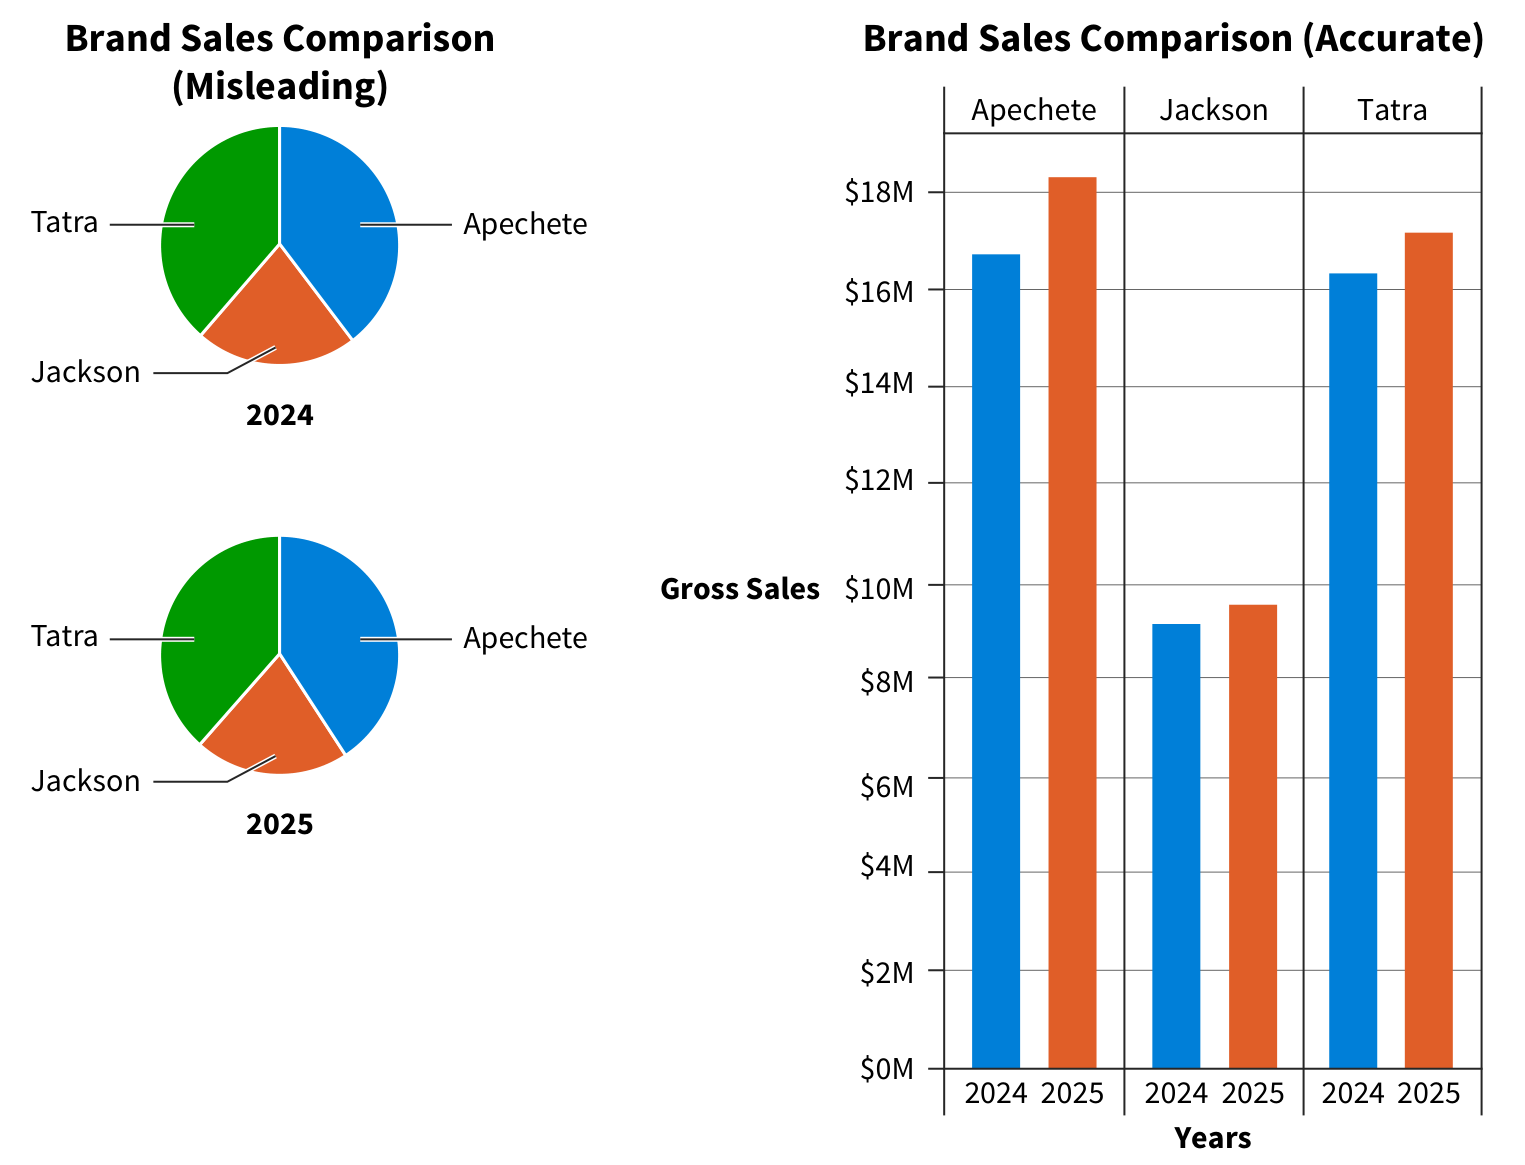
\includegraphics[width=0.95\textwidth,height=0.75\textheight,keepaspectratio]{../textbookForPractice/Figures/Ch_09/ILLUSTRATION 9.46.png}
    \end{figure}
\end{frame}

\begin{frame}{ILLUSTRATION 9.47}

    \begin{figure}[h]
        \centering
        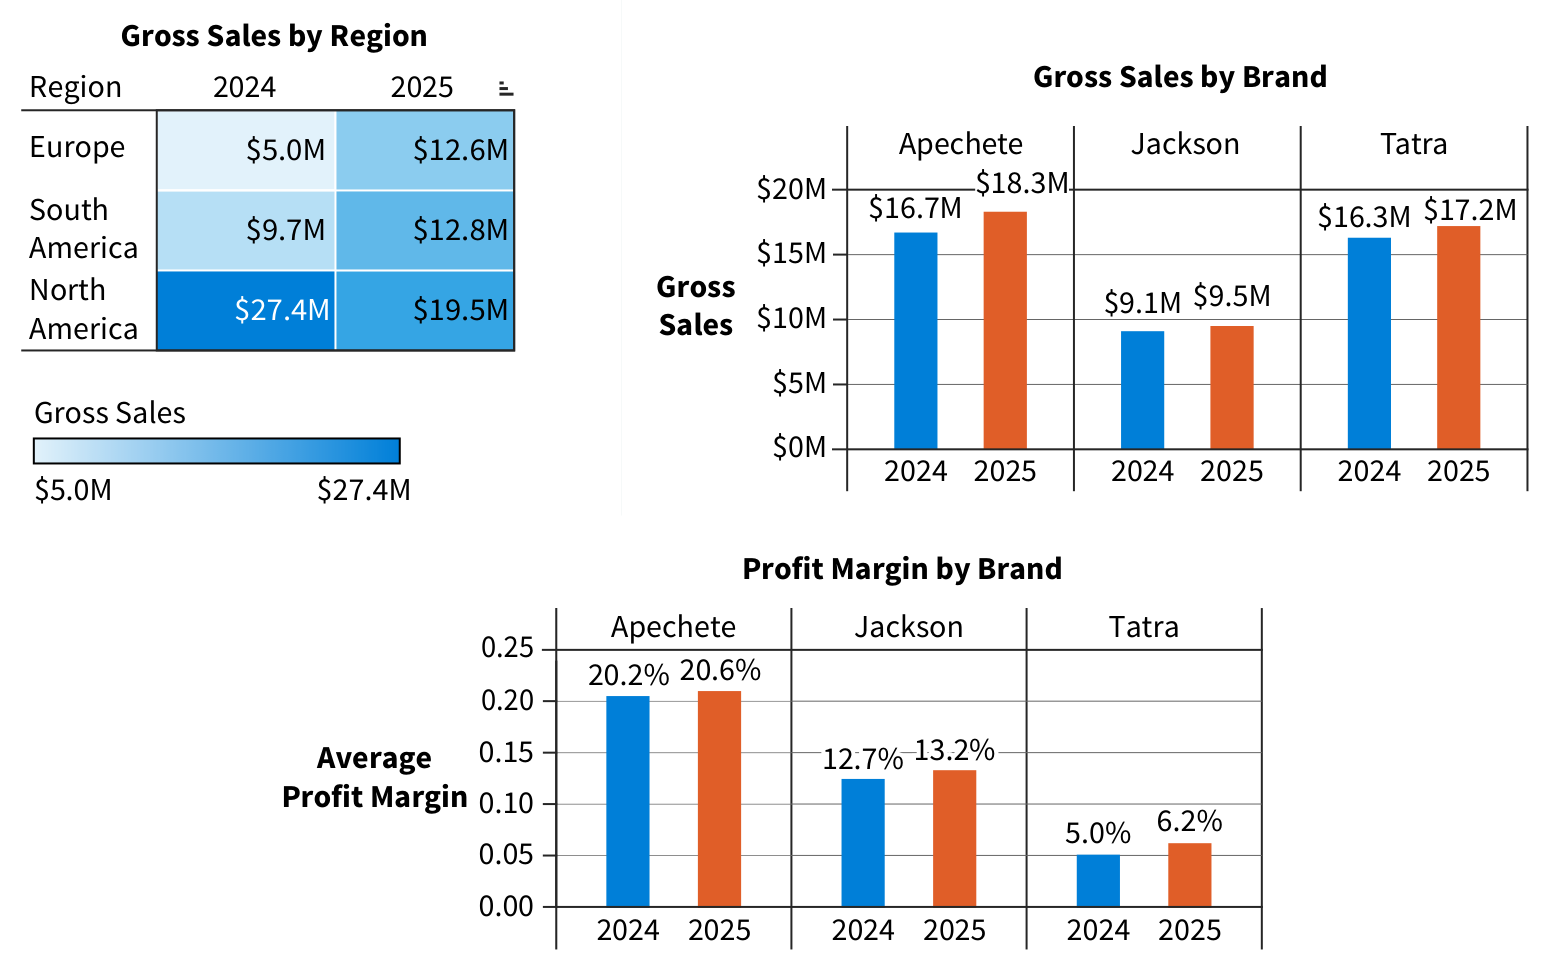
\includegraphics[width=0.95\textwidth,height=0.75\textheight,keepaspectratio]{../textbookForPractice/Figures/Ch_09/ILLUSTRATION 9.47.png}
    \end{figure}
\end{frame}

\begin{frame}{9.5 Thiết Kế Bài Thuyết Trình Tương Tác}
\begin{itemize}
    \item Việc báo cáo bằng file tĩnh truyền thống (PDF, Excel) đang dần nhường chỗ cho các báo cáo tương tác.
    \item \textbf{Interactive Dashboards:} Người dùng có thể click, filter (lọc) và drill-down (đi sâu) để xem dữ liệu theo ý muốn.
\end{itemize}
\end{frame}

\begin{frame}{ILLUSTRATION 9.48}

    \begin{figure}[h]
        \centering
        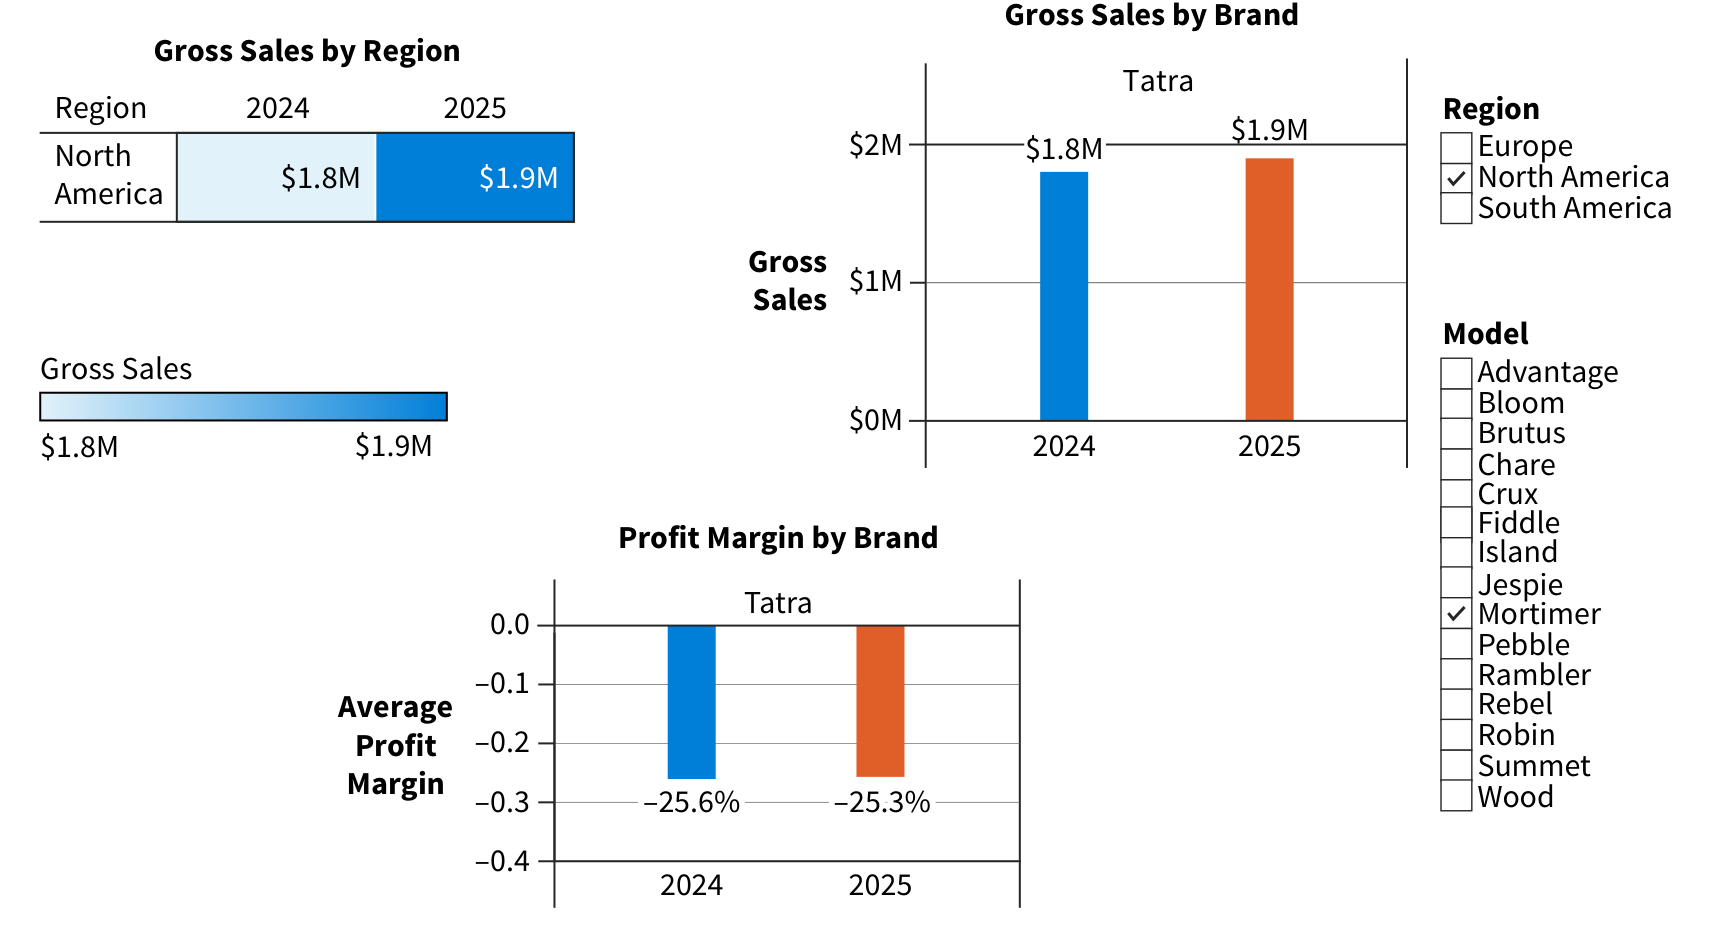
\includegraphics[width=0.95\textwidth,height=0.75\textheight,keepaspectratio]{../textbookForPractice/Figures/Ch_09/ILLUSTRATION 9.48.png}
    \end{figure}
\end{frame}

\begin{frame}{ILLUSTRATION 9.49}

    \begin{figure}[h]
        \centering
        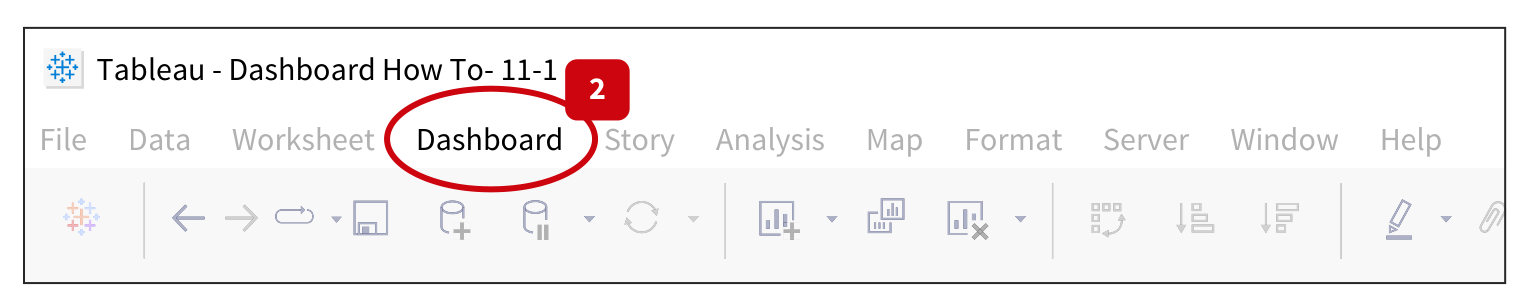
\includegraphics[width=0.95\textwidth,height=0.75\textheight,keepaspectratio]{../textbookForPractice/Figures/Ch_09/ILLUSTRATION 9.49.png}
    \end{figure}
\end{frame}

\begin{frame}{Kinh Nghiệm Thuyết Trình Trực Tiếp}
\begin{itemize}
    \item \textbf{Best Practices for Live Presentations:}
    \item Không đưa quá nhiều chữ lên slide (khán giả sẽ đọc chữ thay vì nghe bạn nói).
    \item Sử dụng biểu đồ để hỗ trợ lập luận. Giải thích rõ các trục tung/hoành trước khi phân tích xu hướng.
\end{itemize}
\end{frame}

\begin{frame}{ILLUSTRATION 9.50}

    \begin{figure}[h]
        \centering
        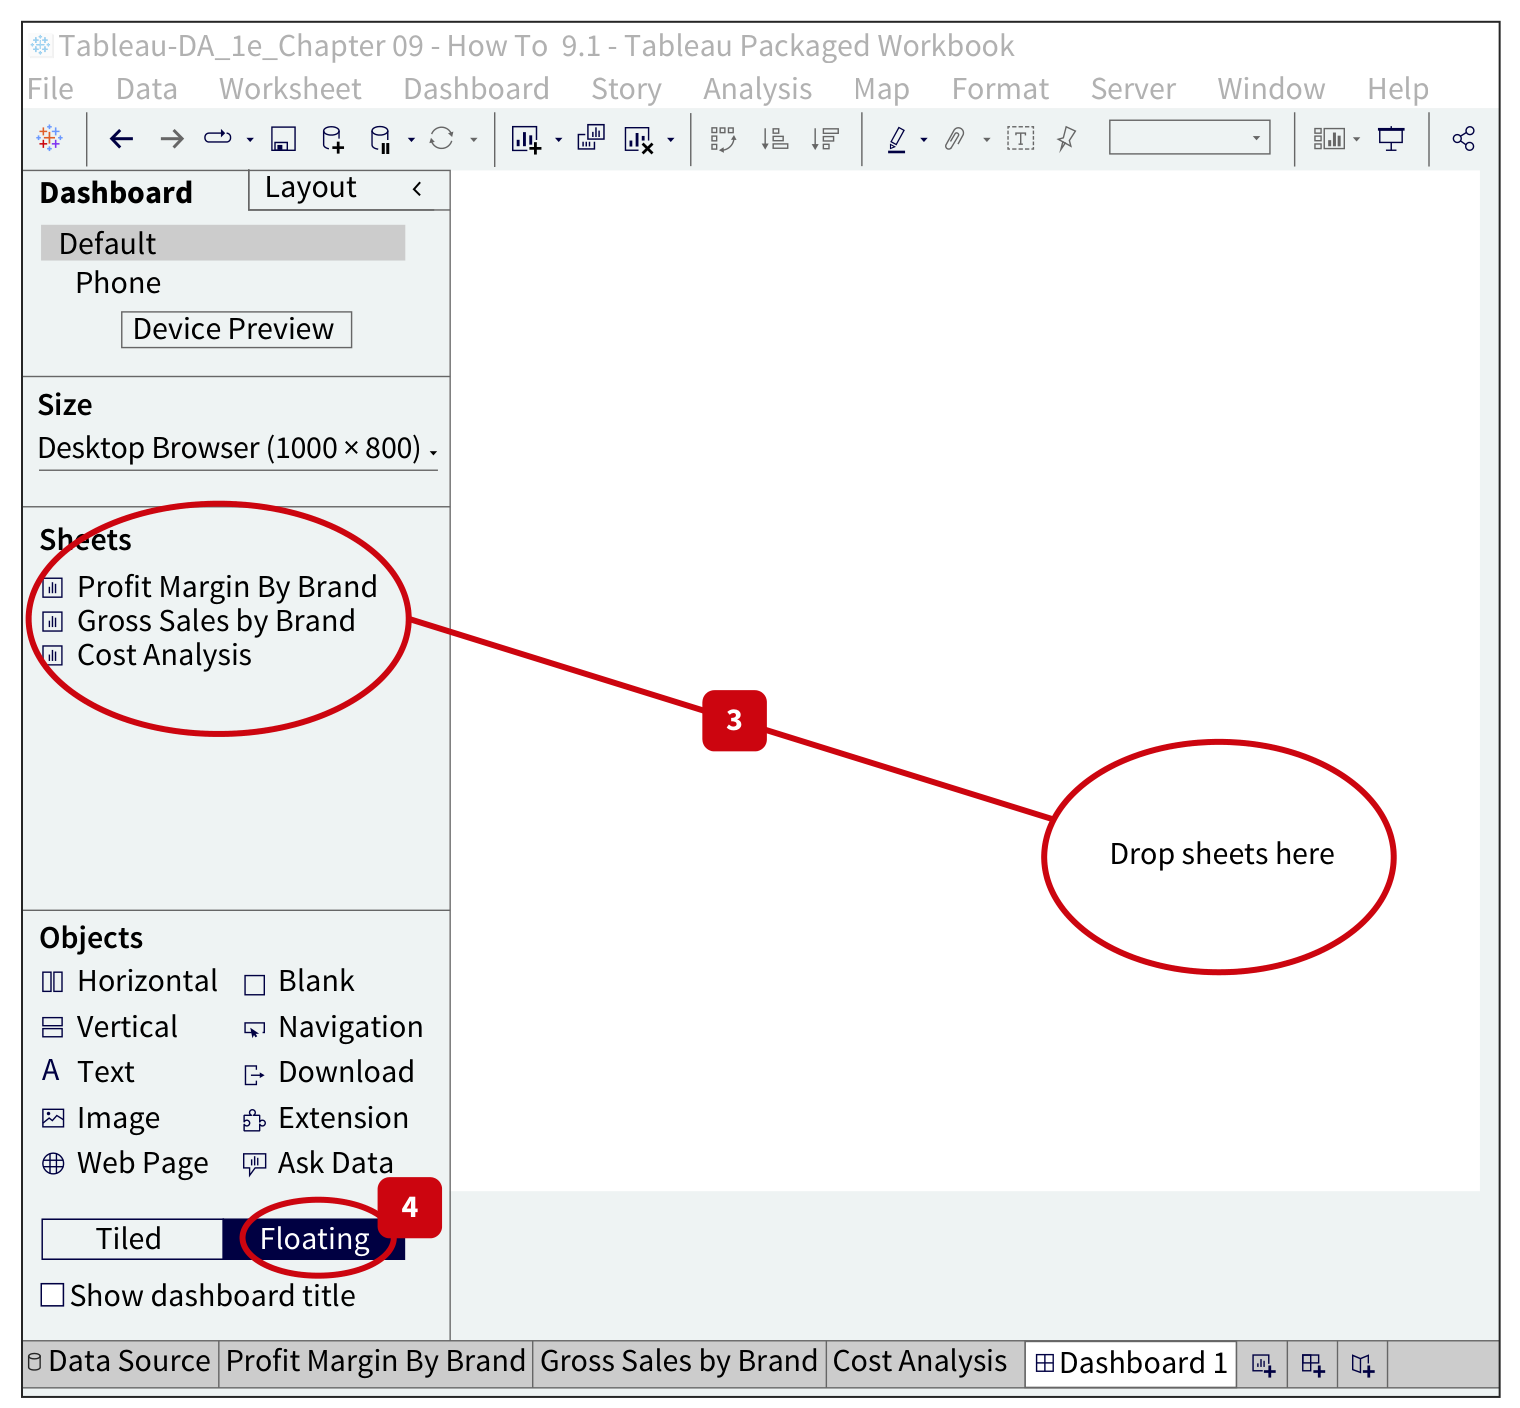
\includegraphics[width=0.95\textwidth,height=0.75\textheight,keepaspectratio]{../textbookForPractice/Figures/Ch_09/ILLUSTRATION 9.50.png}
    \end{figure}
\end{frame}

\begin{frame}{ILLUSTRATION 9.51}

    \begin{figure}[h]
        \centering
        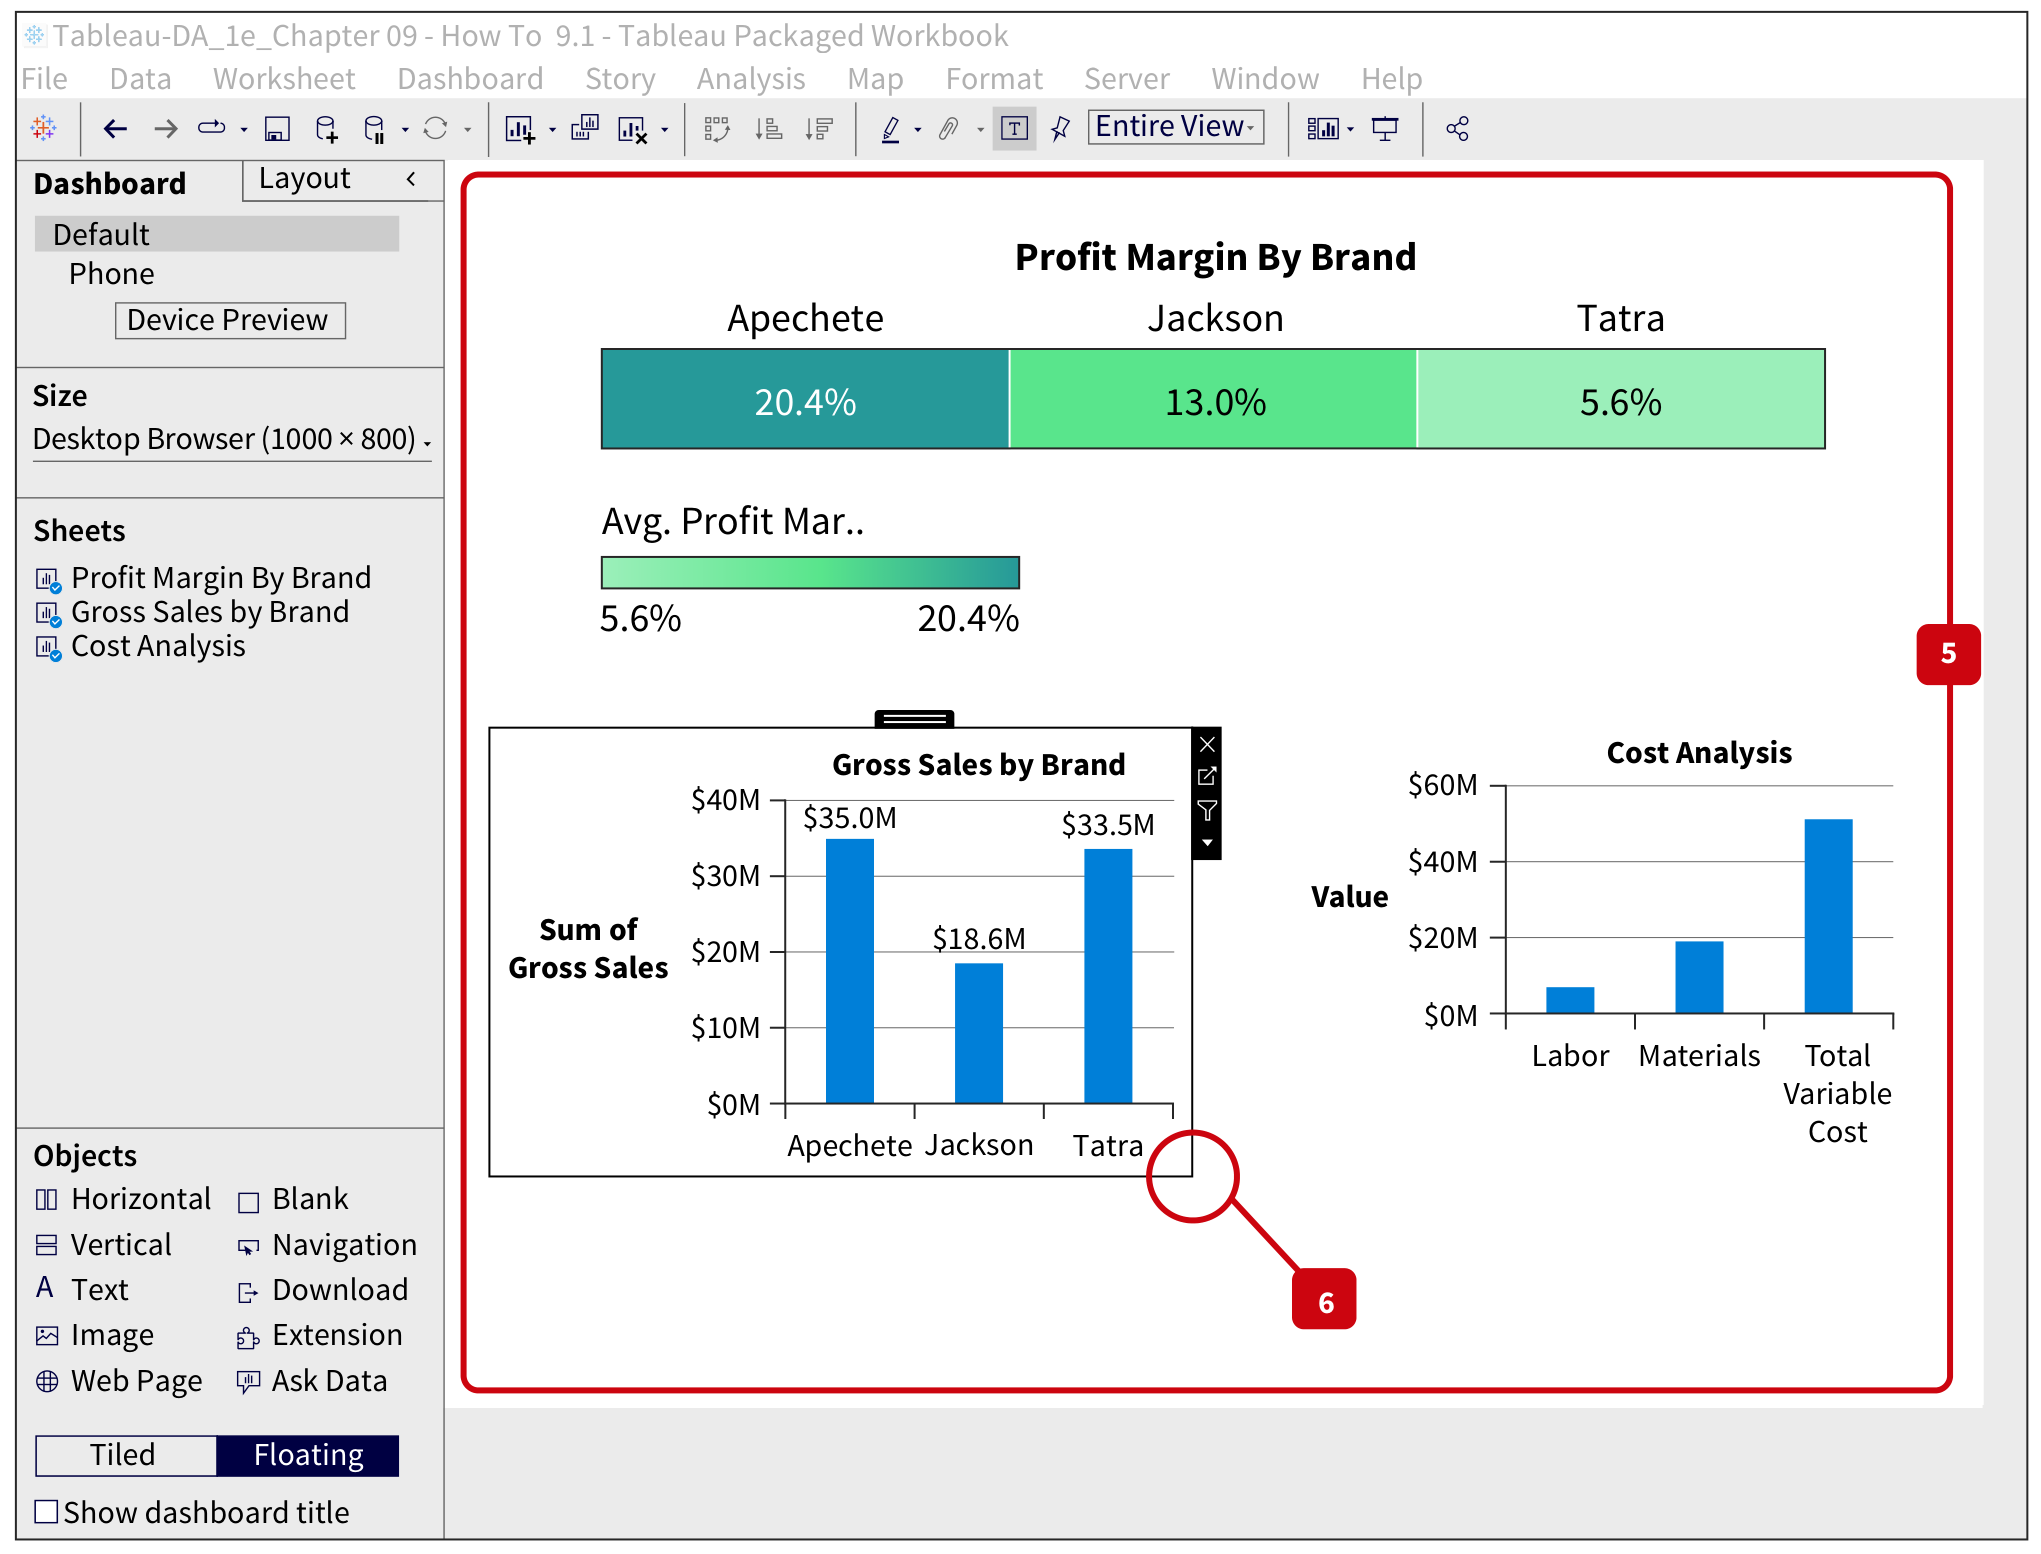
\includegraphics[width=0.95\textwidth,height=0.75\textheight,keepaspectratio]{../textbookForPractice/Figures/Ch_09/ILLUSTRATION 9.51.png}
    \end{figure}
\end{frame}

\begin{frame}{Case Study: Báo Cáo Kế Toán Trực Quan}
\begin{itemize}
    \item Ứng dụng xây dựng Dashboard trong các cơ quan nhà nước, thư viện công cộng (VD: Madison Public Library) và doanh nghiệp.
    \item Cho phép Ban Giám đốc nhìn được bức tranh thu-chi và phân bổ ngân sách real-time.
\end{itemize}
\end{frame}

\begin{frame}{ILLUSTRATION 9.52}

    \begin{figure}[h]
        \centering
        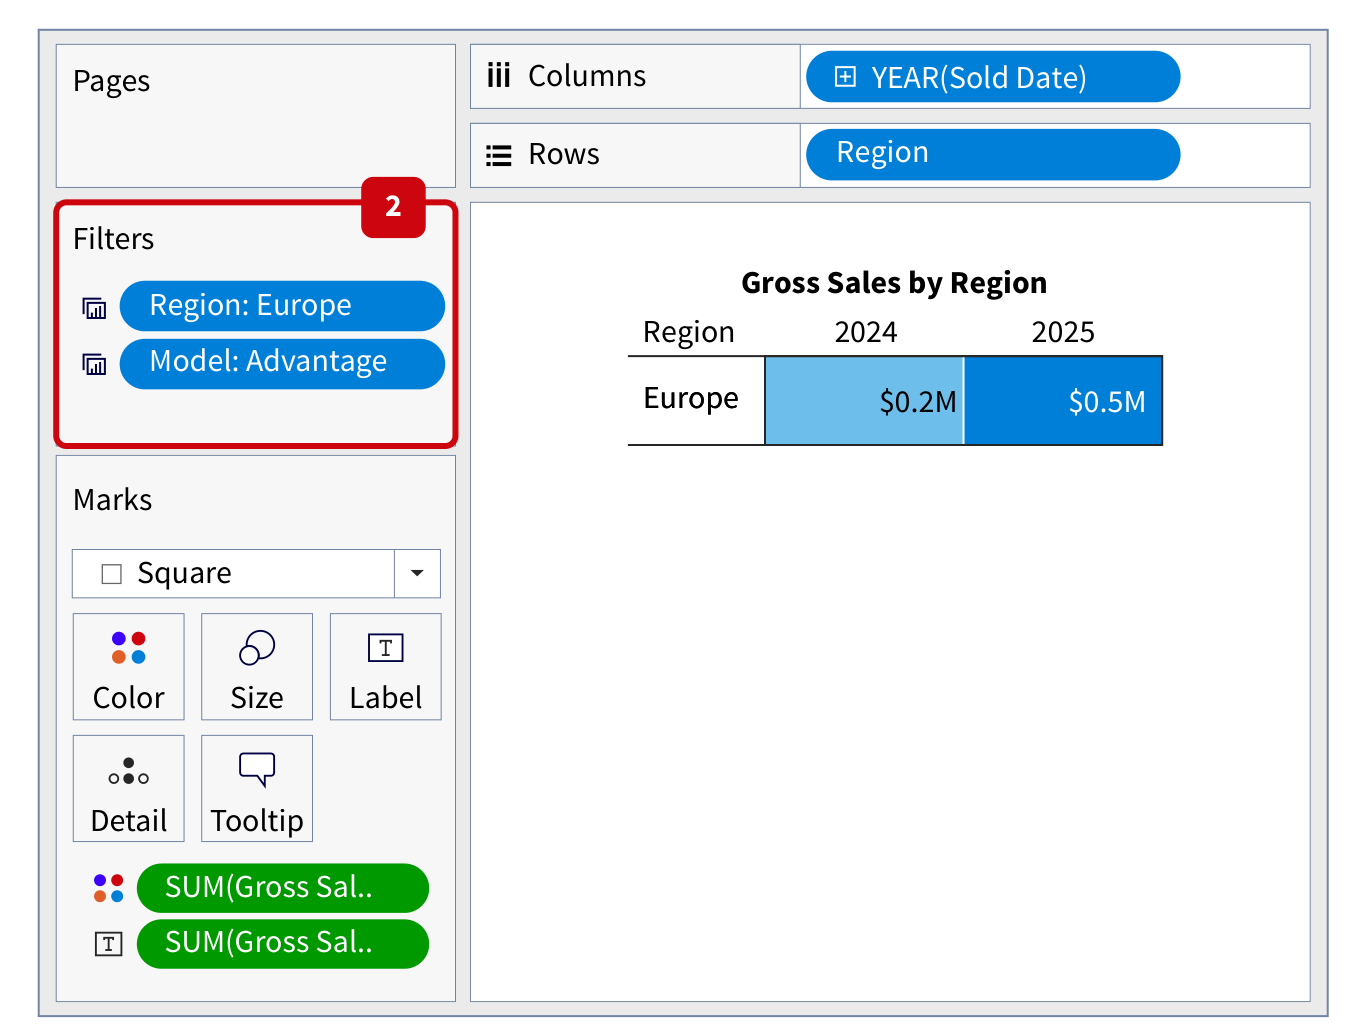
\includegraphics[width=0.95\textwidth,height=0.75\textheight,keepaspectratio]{../textbookForPractice/Figures/Ch_09/ILLUSTRATION 9.52.png}
    \end{figure}
\end{frame}

\begin{frame}{ILLUSTRATION 9.53A}

    \begin{figure}[h]
        \centering
        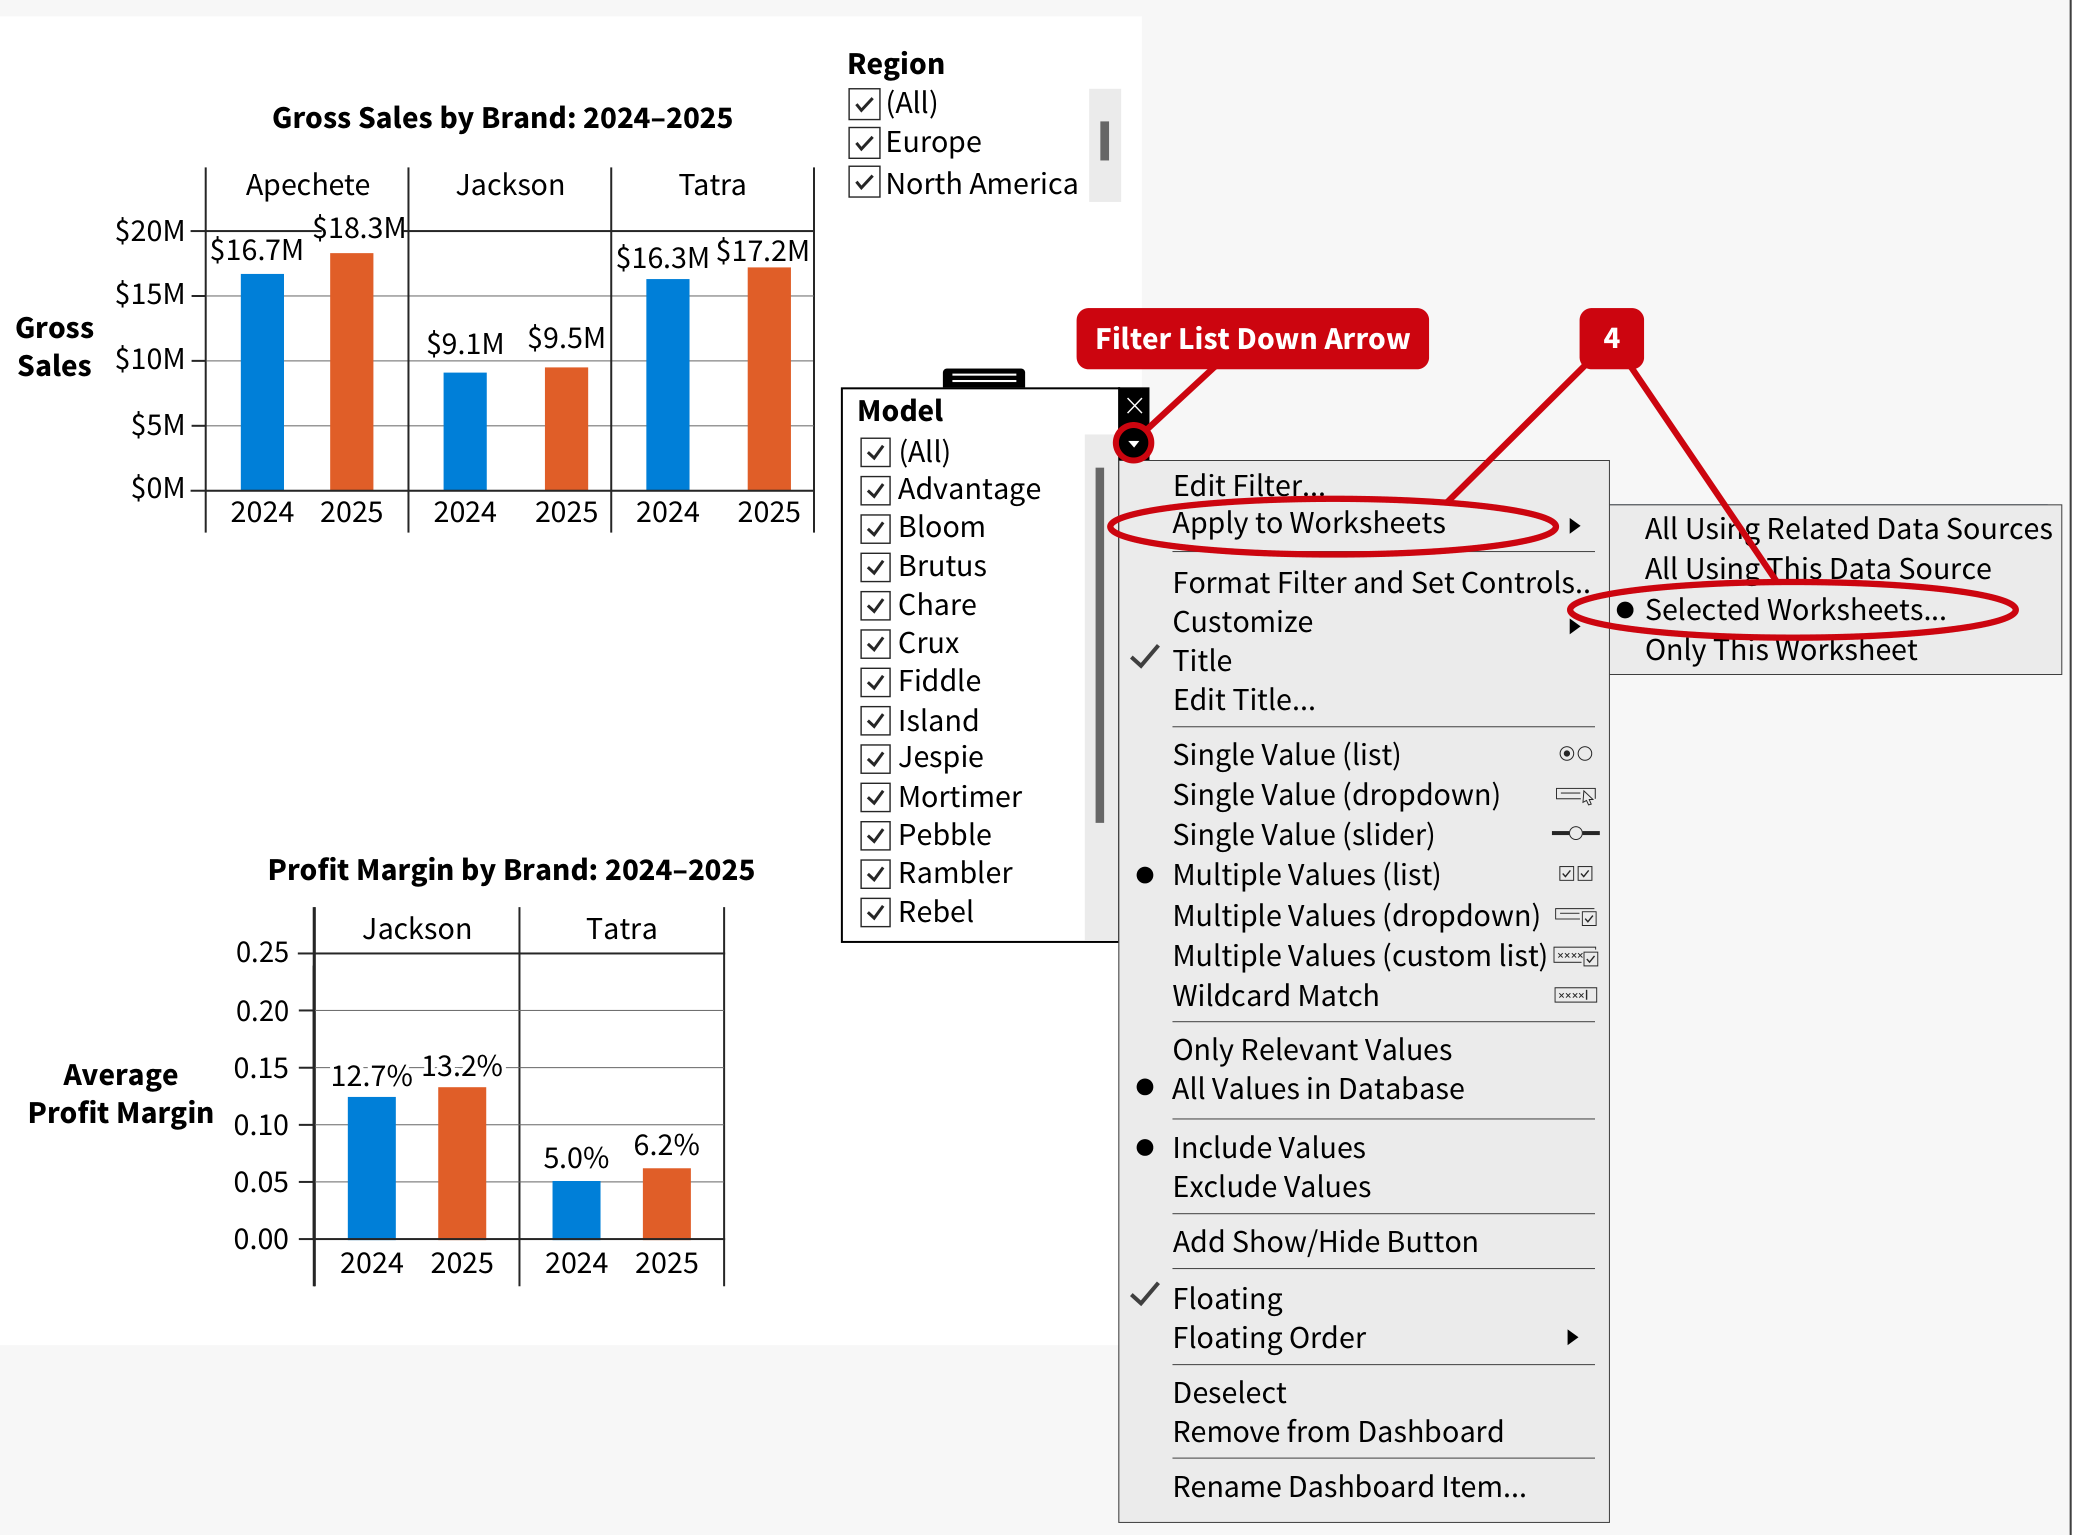
\includegraphics[width=0.95\textwidth,height=0.75\textheight,keepaspectratio]{../textbookForPractice/Figures/Ch_09/ILLUSTRATION 9.53A.png}
    \end{figure}
\end{frame}

\begin{frame}{Tổng Kết Chương}
\begin{itemize}
    \item \textbf{Tóm tắt LO 9.1 - LO 9.5:} Kỹ năng phân tích dữ liệu không chỉ nằm ở việc xử lý kỹ thuật, mà quan trọng nhất là \textbf{truyền đạt (communicate)} được giá trị của dữ liệu.
    \item Trực quan hóa đúng cách giúp tối ưu hóa ra quyết định.
\end{itemize}
\end{frame}

\begin{frame}{ILLUSTRATION 9.53B}

    \begin{figure}[h]
        \centering
        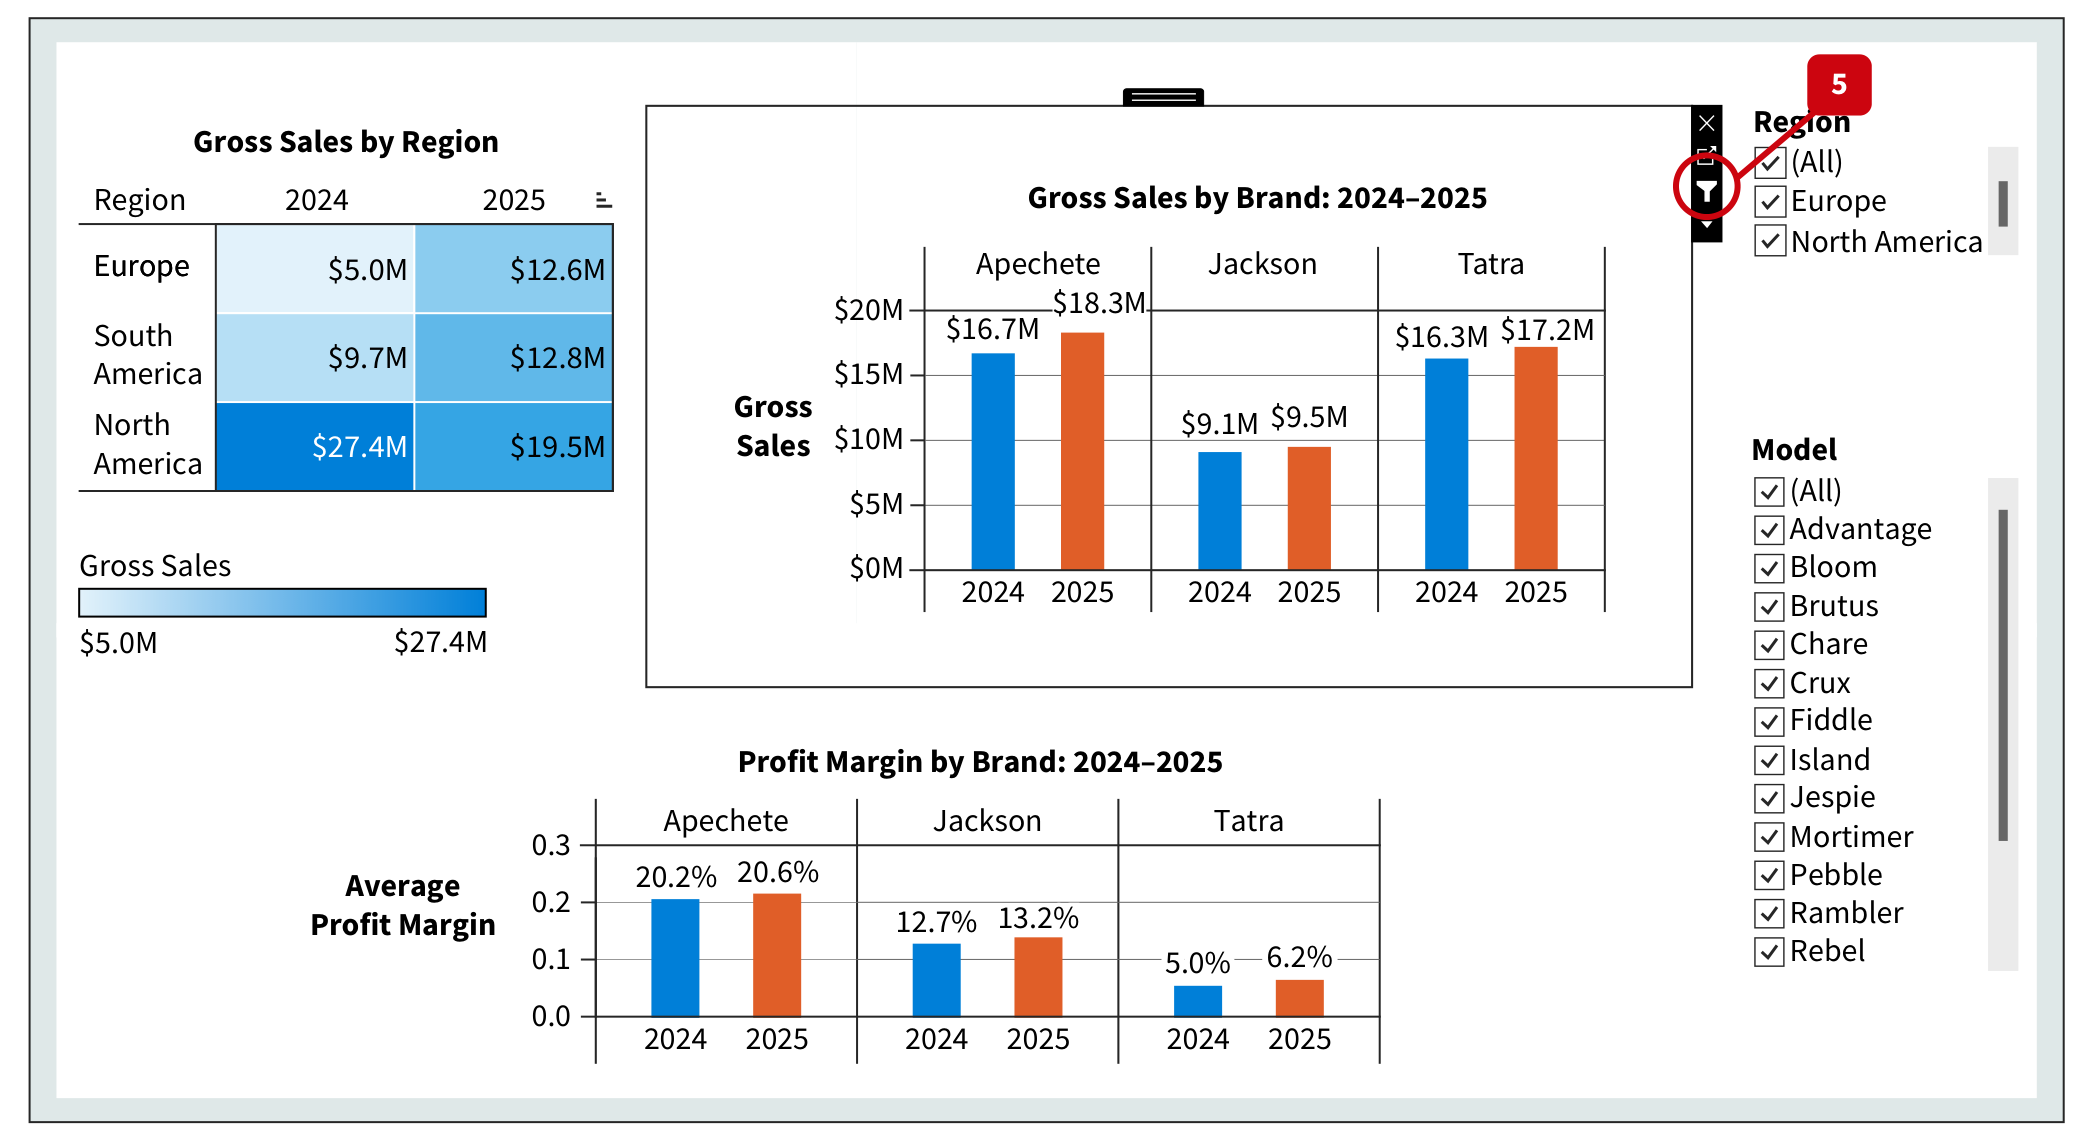
\includegraphics[width=0.95\textwidth,height=0.75\textheight,keepaspectratio]{../textbookForPractice/Figures/Ch_09/ILLUSTRATION 9.53B.png}
    \end{figure}
\end{frame}

\begin{frame}{ILLUSTRATION 9.55}

    \begin{figure}[h]
        \centering
        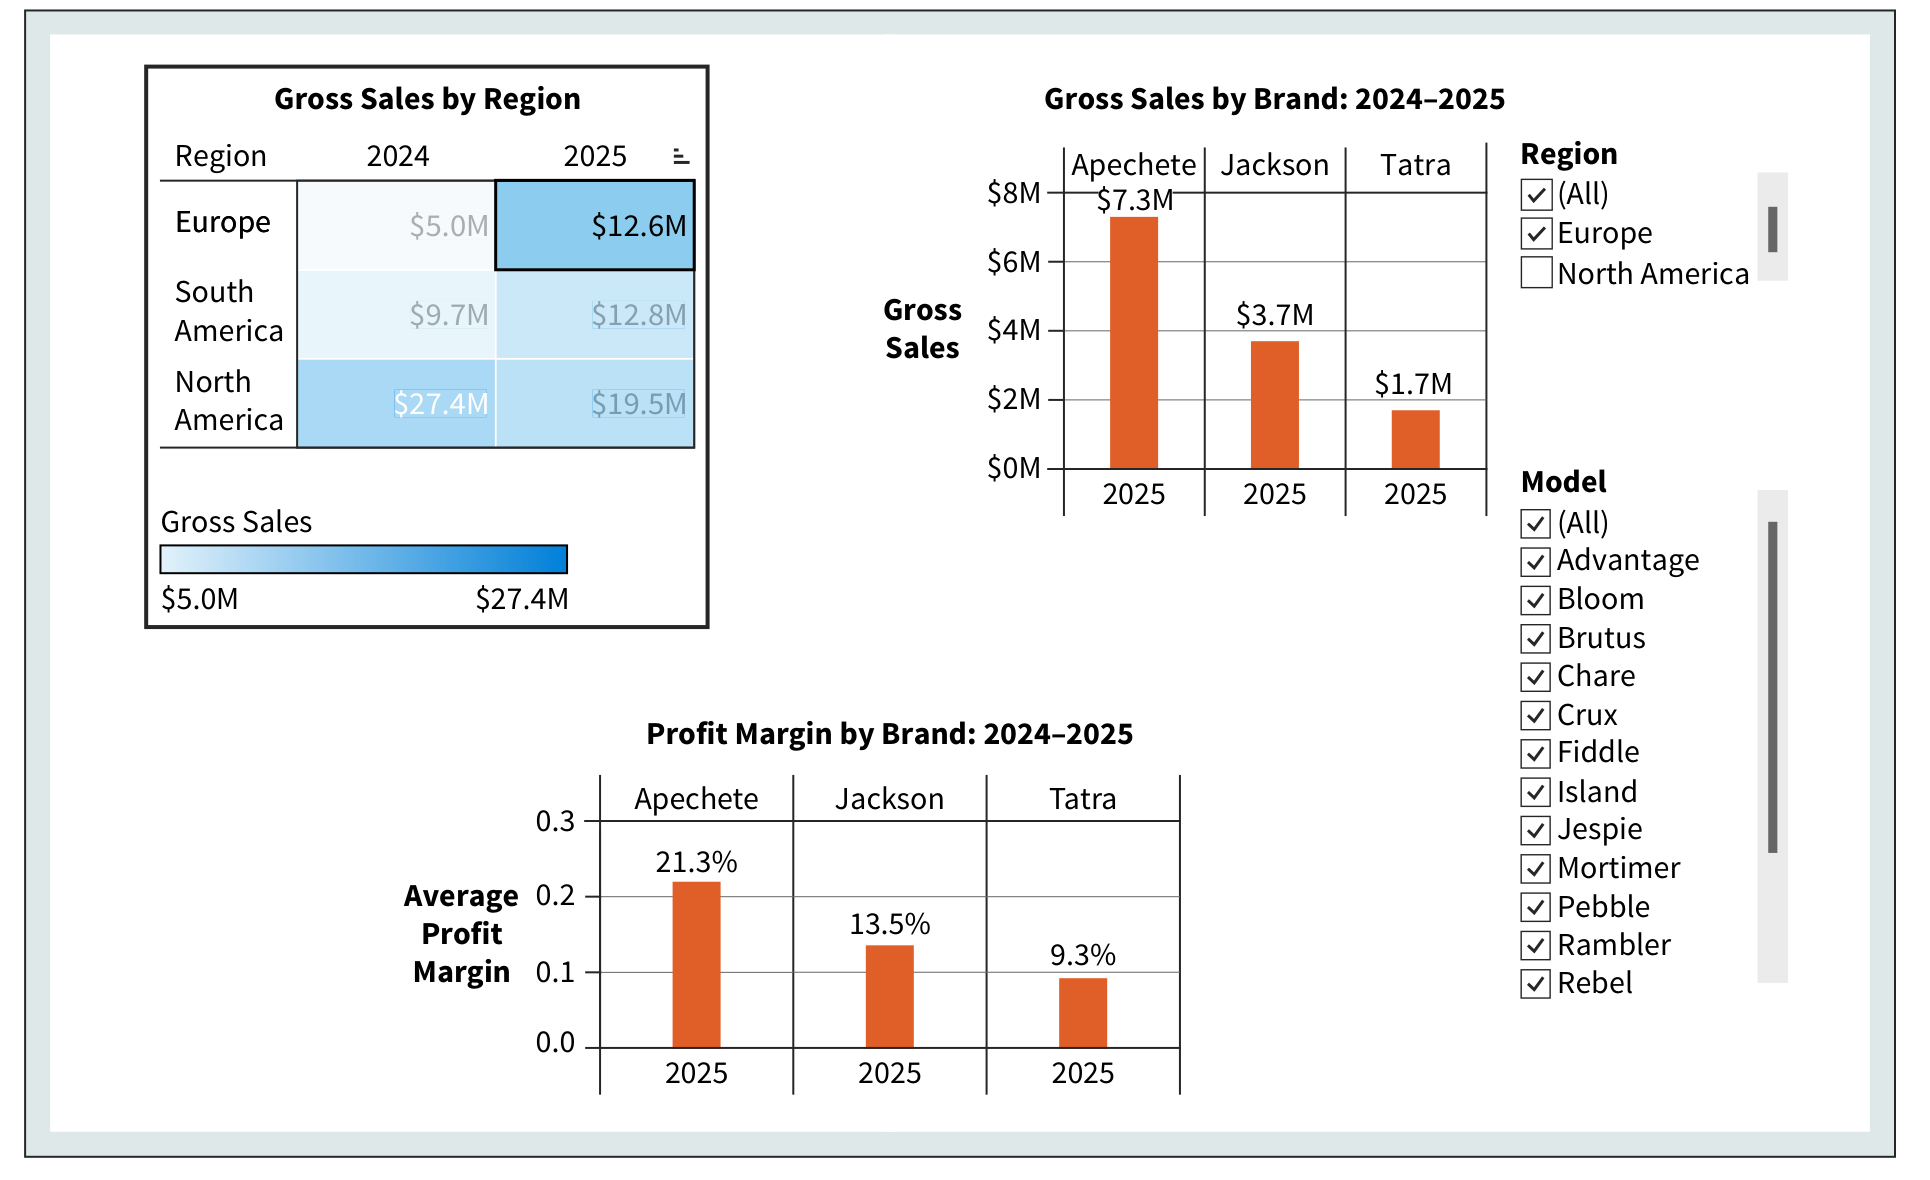
\includegraphics[width=0.95\textwidth,height=0.75\textheight,keepaspectratio]{../textbookForPractice/Figures/Ch_09/ILLUSTRATION 9.55.png}
    \end{figure}
\end{frame}

\begin{frame}{LO 4.15}

    \begin{figure}[h]
        \centering
        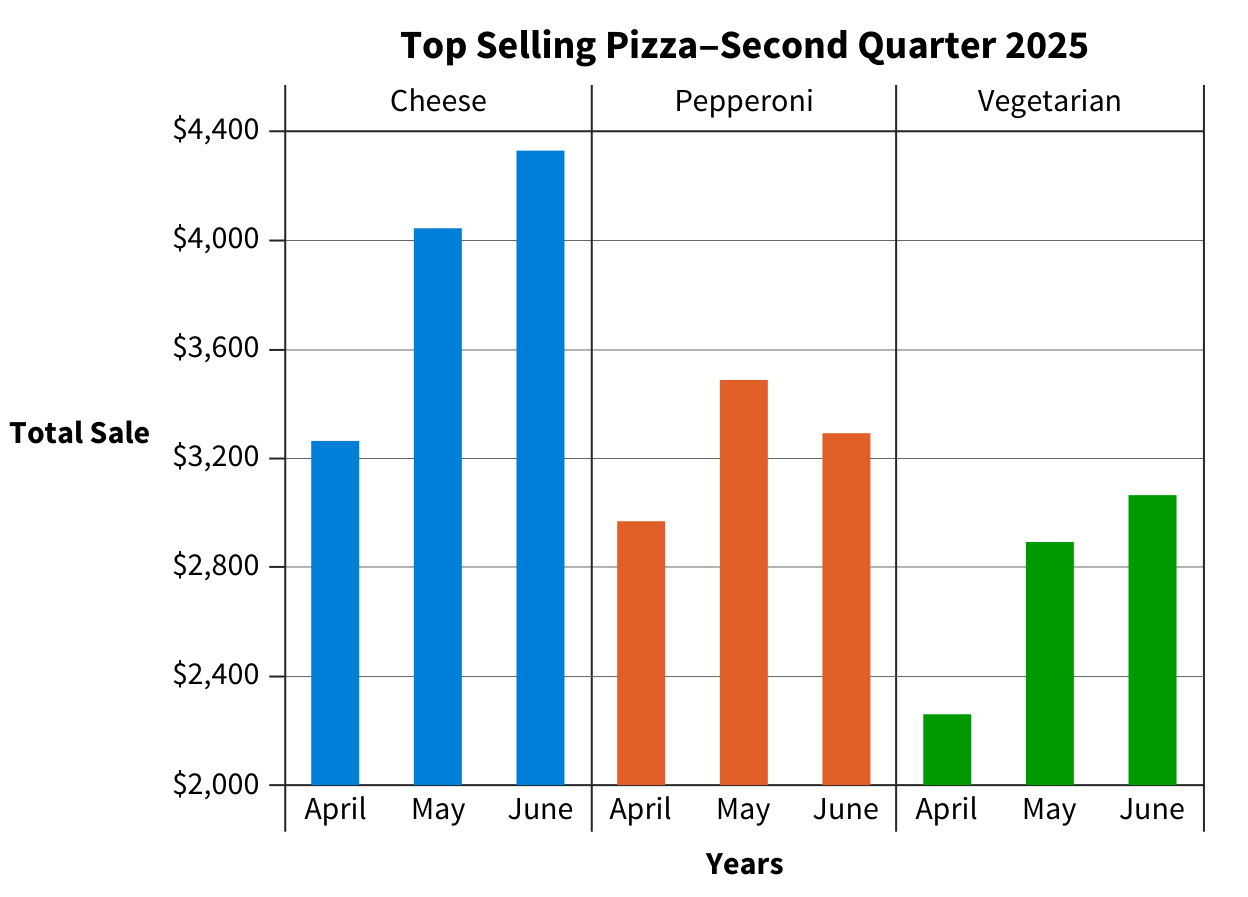
\includegraphics[width=0.95\textwidth,height=0.75\textheight,keepaspectratio]{../textbookForPractice/Figures/Ch_09/LO 4.15.png}
    \end{figure}
\end{frame}

\begin{frame}{LO 4.16}

    \begin{figure}[h]
        \centering
        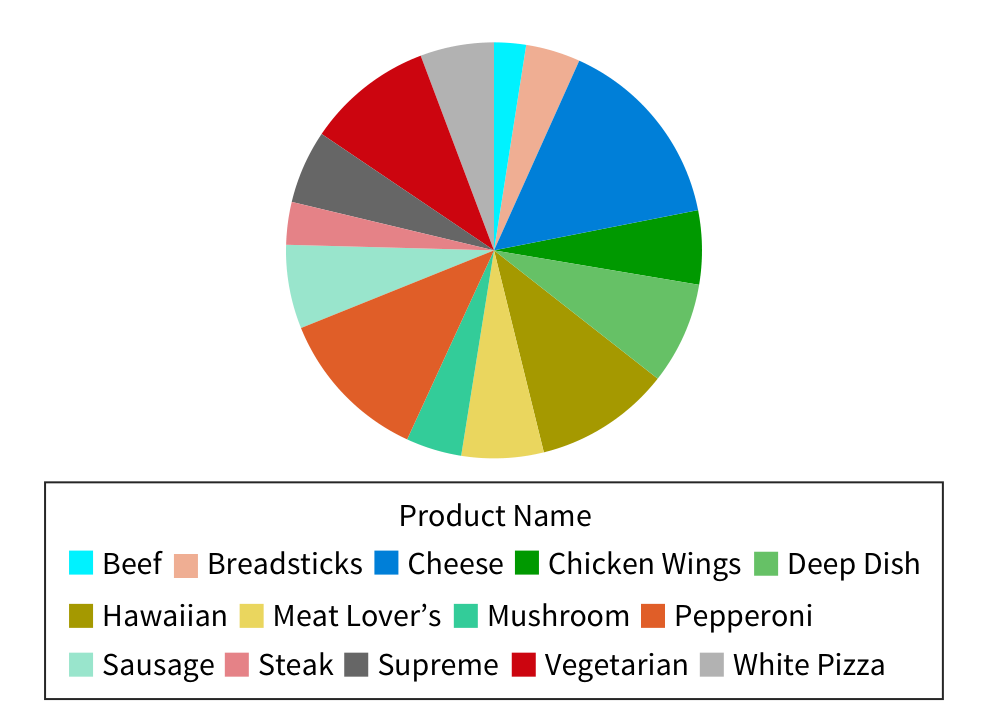
\includegraphics[width=0.95\textwidth,height=0.75\textheight,keepaspectratio]{../textbookForPractice/Figures/Ch_09/LO 4.16.png}
    \end{figure}
\end{frame}

\begin{frame}{LO 4.17}

    \begin{figure}[h]
        \centering
        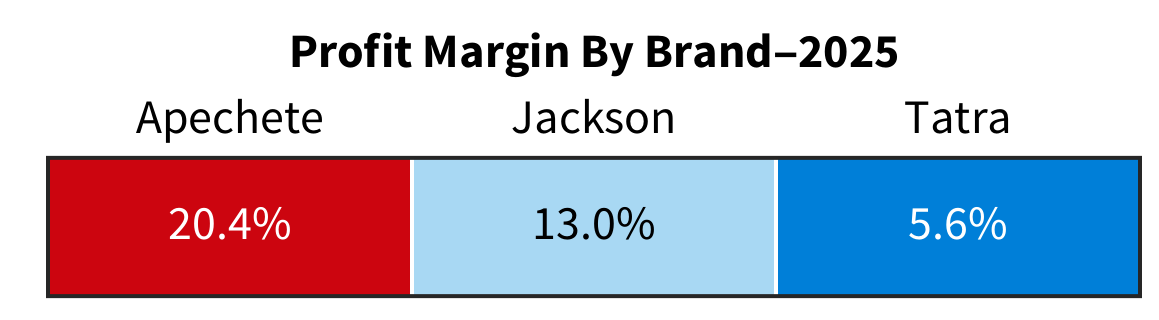
\includegraphics[width=0.95\textwidth,height=0.75\textheight,keepaspectratio]{../textbookForPractice/Figures/Ch_09/LO 4.17.png}
    \end{figure}
\end{frame}

\begin{frame}{Apply It 9.1}

    \begin{figure}[h]
        \centering
        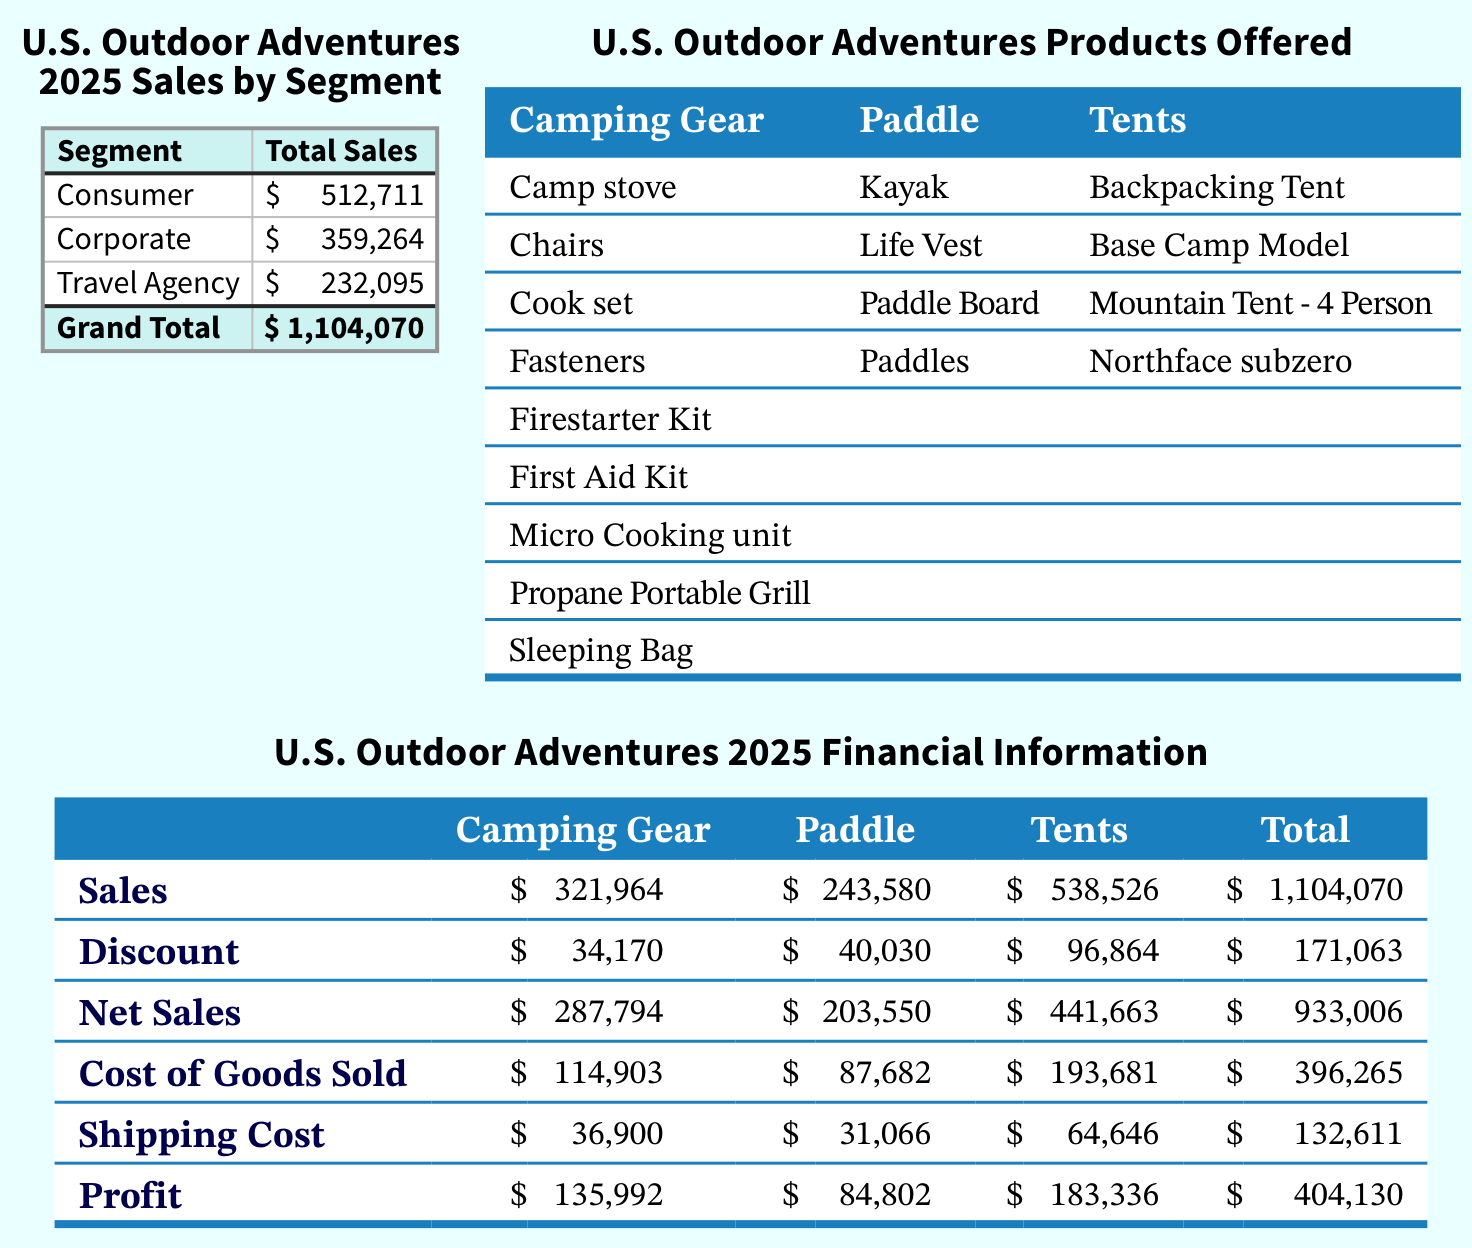
\includegraphics[width=0.95\textwidth,height=0.75\textheight,keepaspectratio]{../textbookForPractice/Figures/Ch_09/Apply It 9.1.png}
    \end{figure}
\end{frame}

\begin{frame}{Madison public library 9.1}

    \begin{figure}[h]
        \centering
        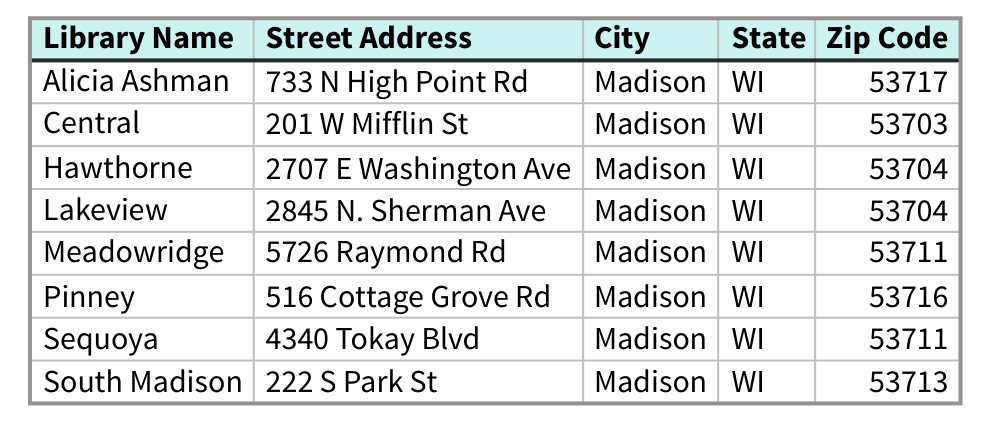
\includegraphics[width=0.95\textwidth,height=0.75\textheight,keepaspectratio]{../textbookForPractice/Figures/Ch_09/Madison public library 9.1.png}
    \end{figure}
\end{frame}

\begin{frame}{Apply It 9.2}

    \begin{figure}[h]
        \centering
        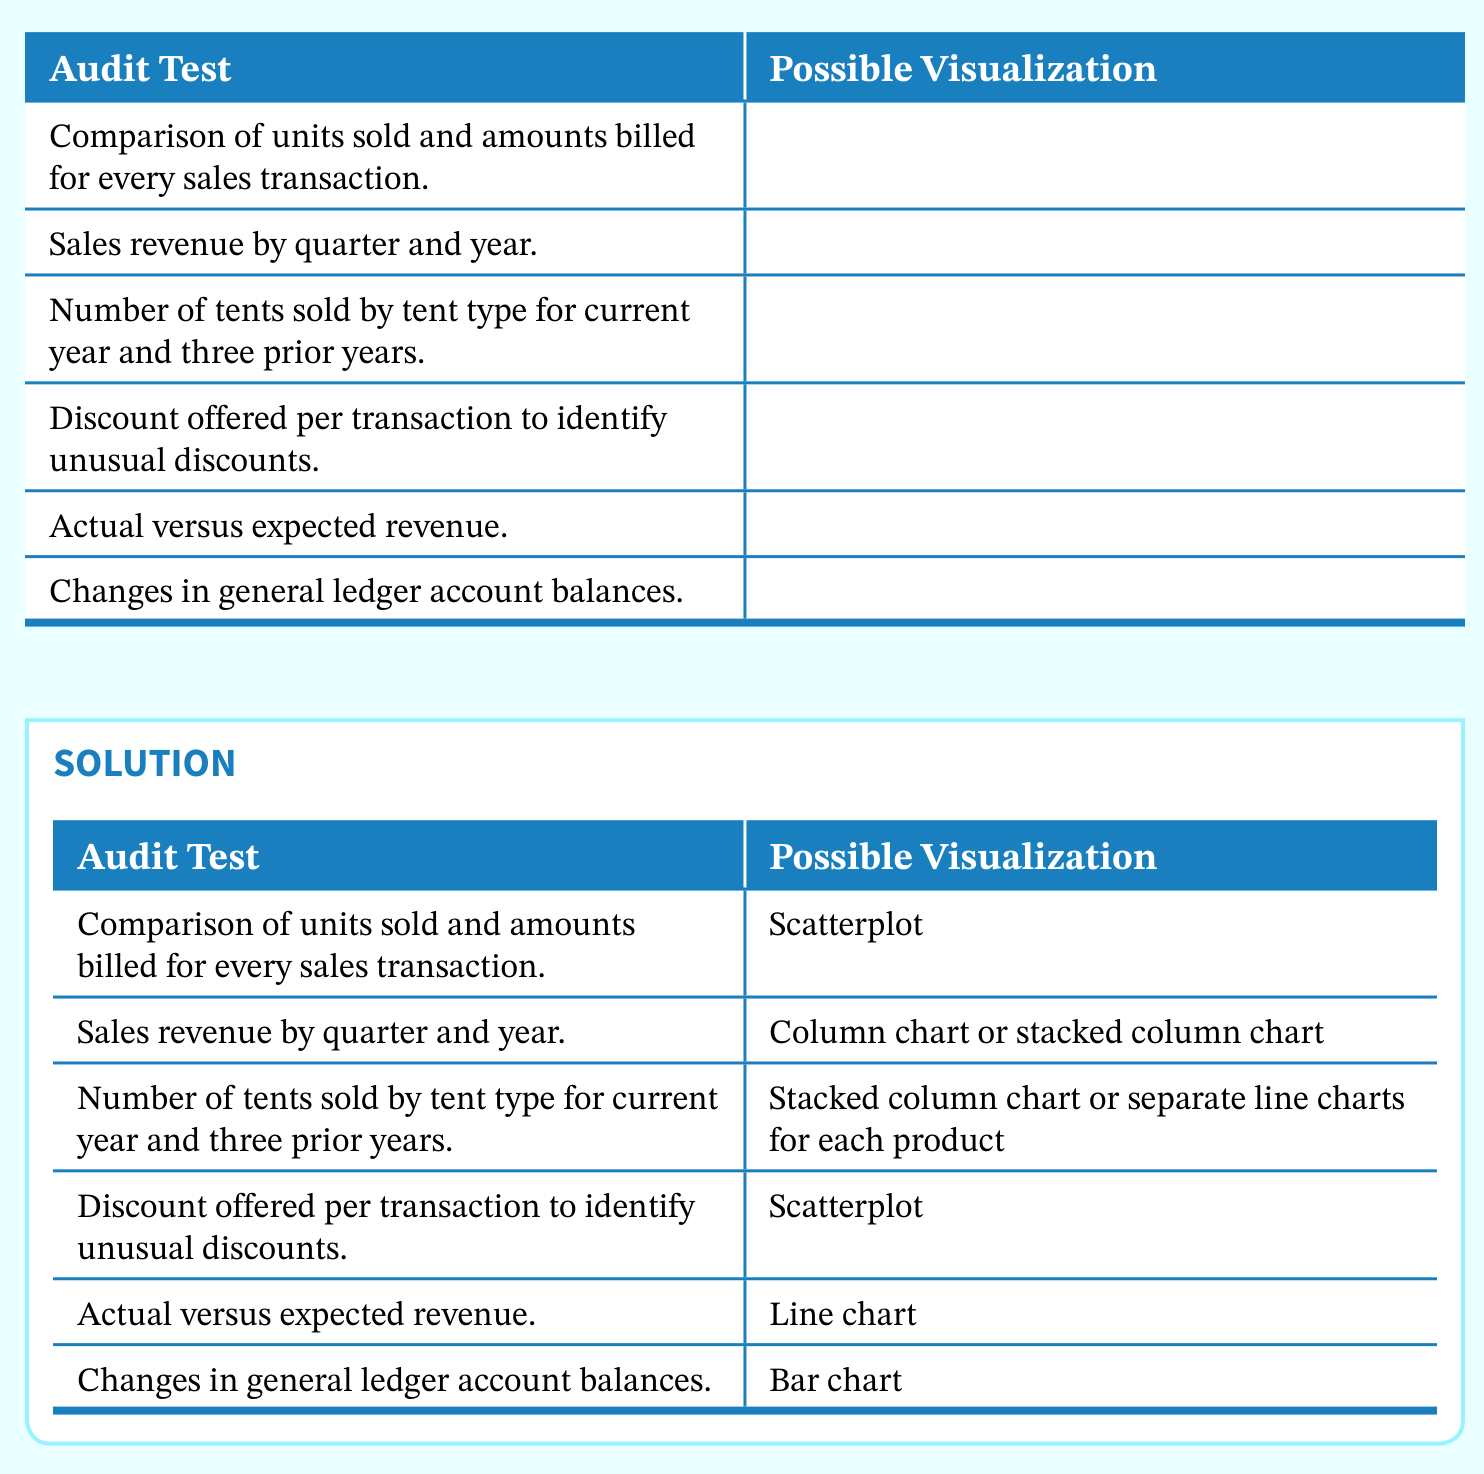
\includegraphics[width=0.95\textwidth,height=0.75\textheight,keepaspectratio]{../textbookForPractice/Figures/Ch_09/Apply It 9.2.png}
    \end{figure}
\end{frame}

\begin{frame}{Madison public library 9.2}

    \begin{figure}[h]
        \centering
        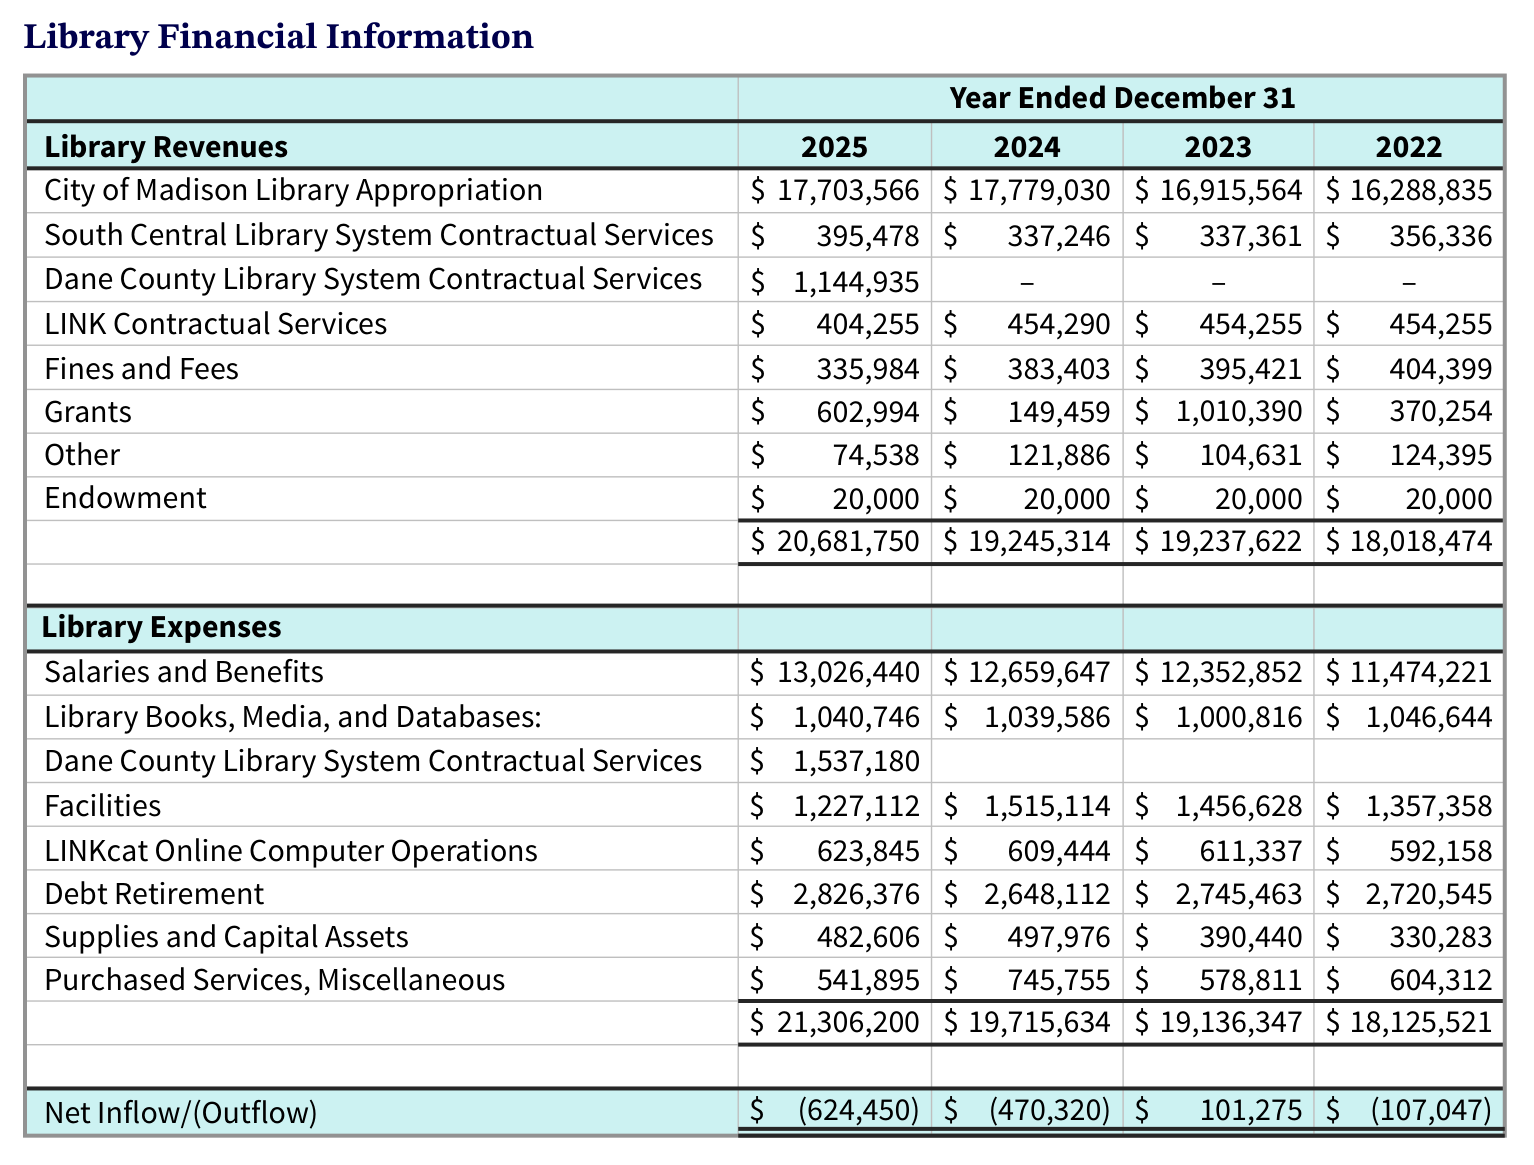
\includegraphics[width=0.95\textwidth,height=0.75\textheight,keepaspectratio]{../textbookForPractice/Figures/Ch_09/Madison public library 9.2.png}
    \end{figure}
\end{frame}

\begin{frame}{Apply It 9.3A}

    \begin{figure}[h]
        \centering
        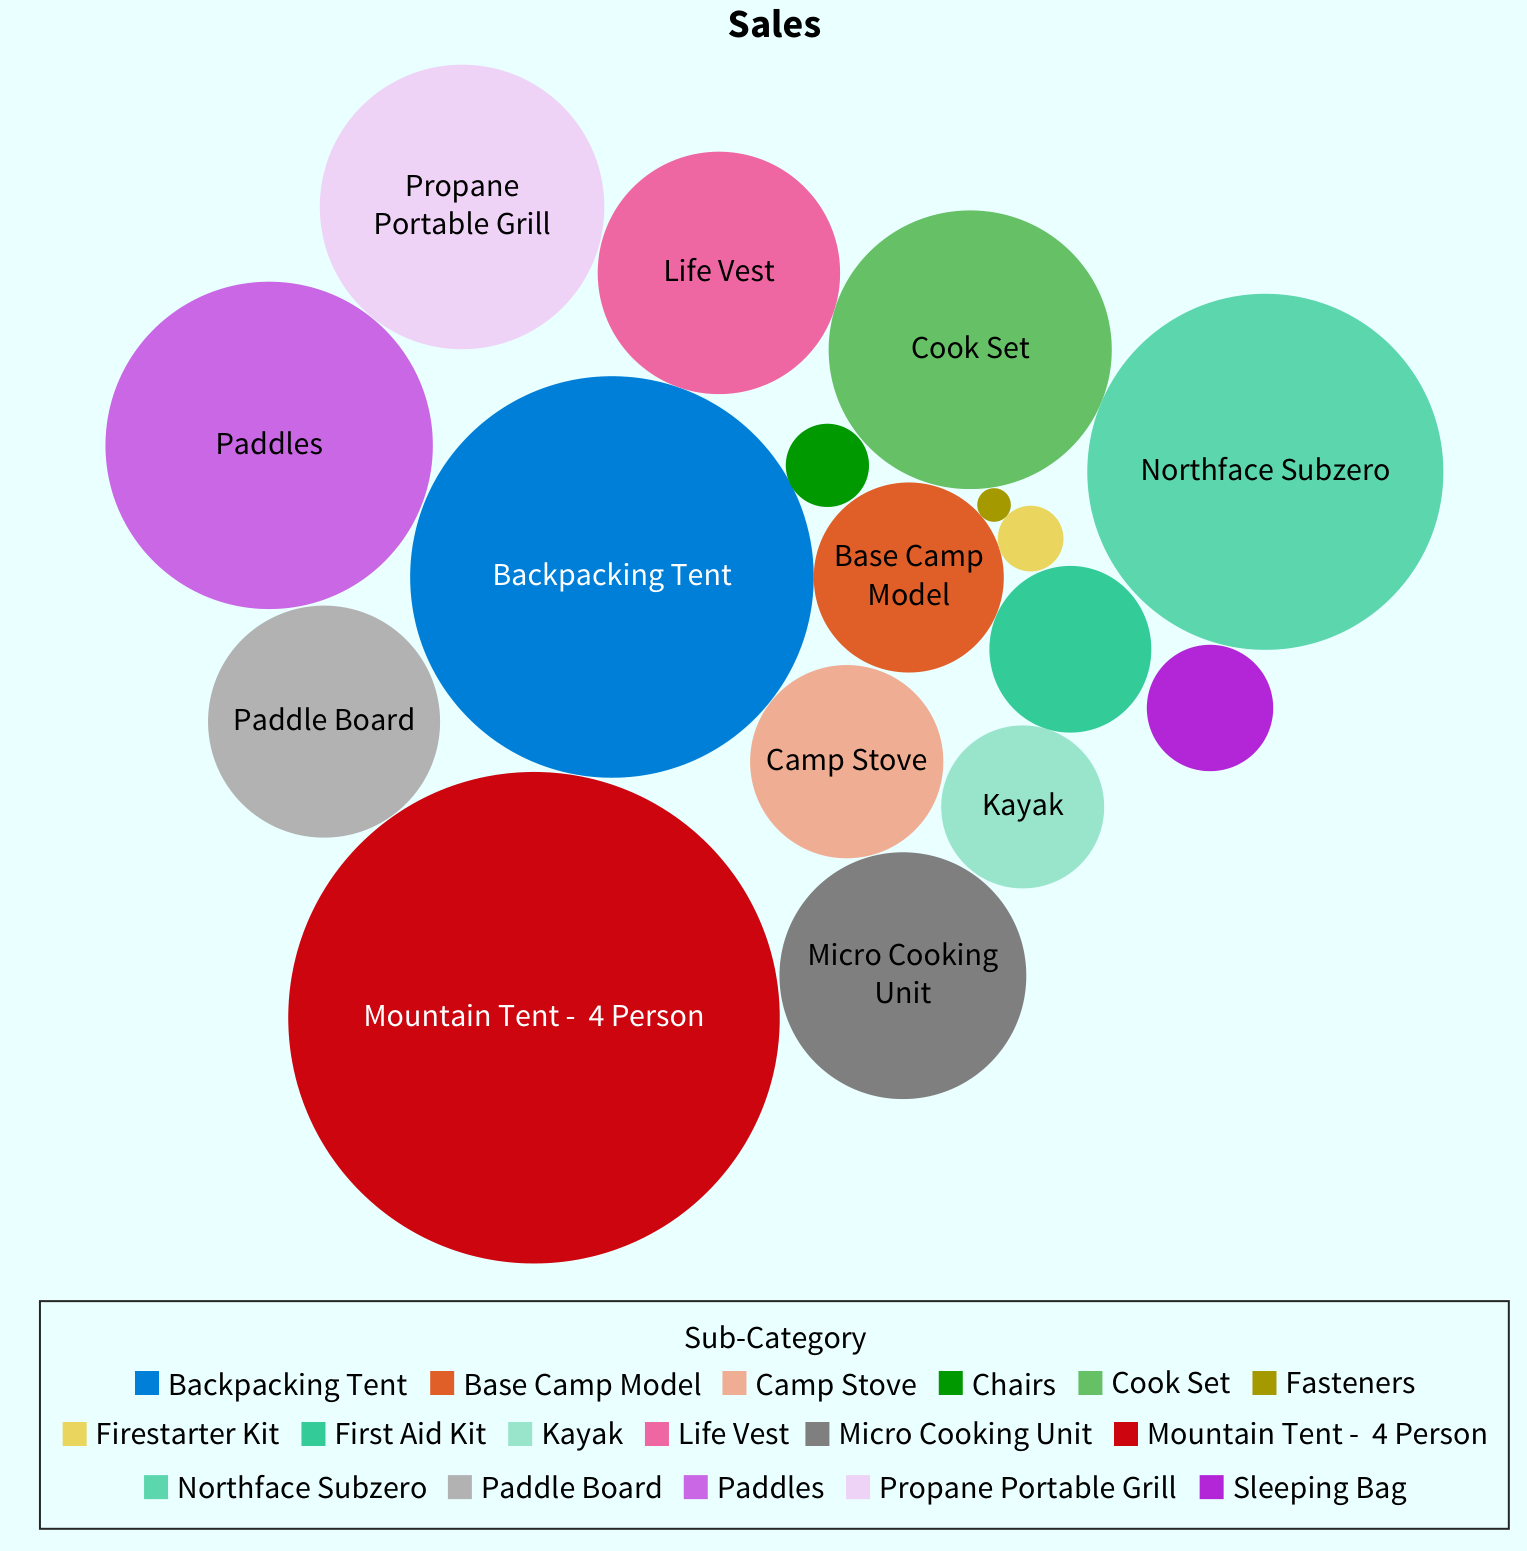
\includegraphics[width=0.95\textwidth,height=0.75\textheight,keepaspectratio]{../textbookForPractice/Figures/Ch_09/Apply It 9.3A.png}
    \end{figure}
\end{frame}

\begin{frame}{Apply It 9.3B}

    \begin{figure}[h]
        \centering
        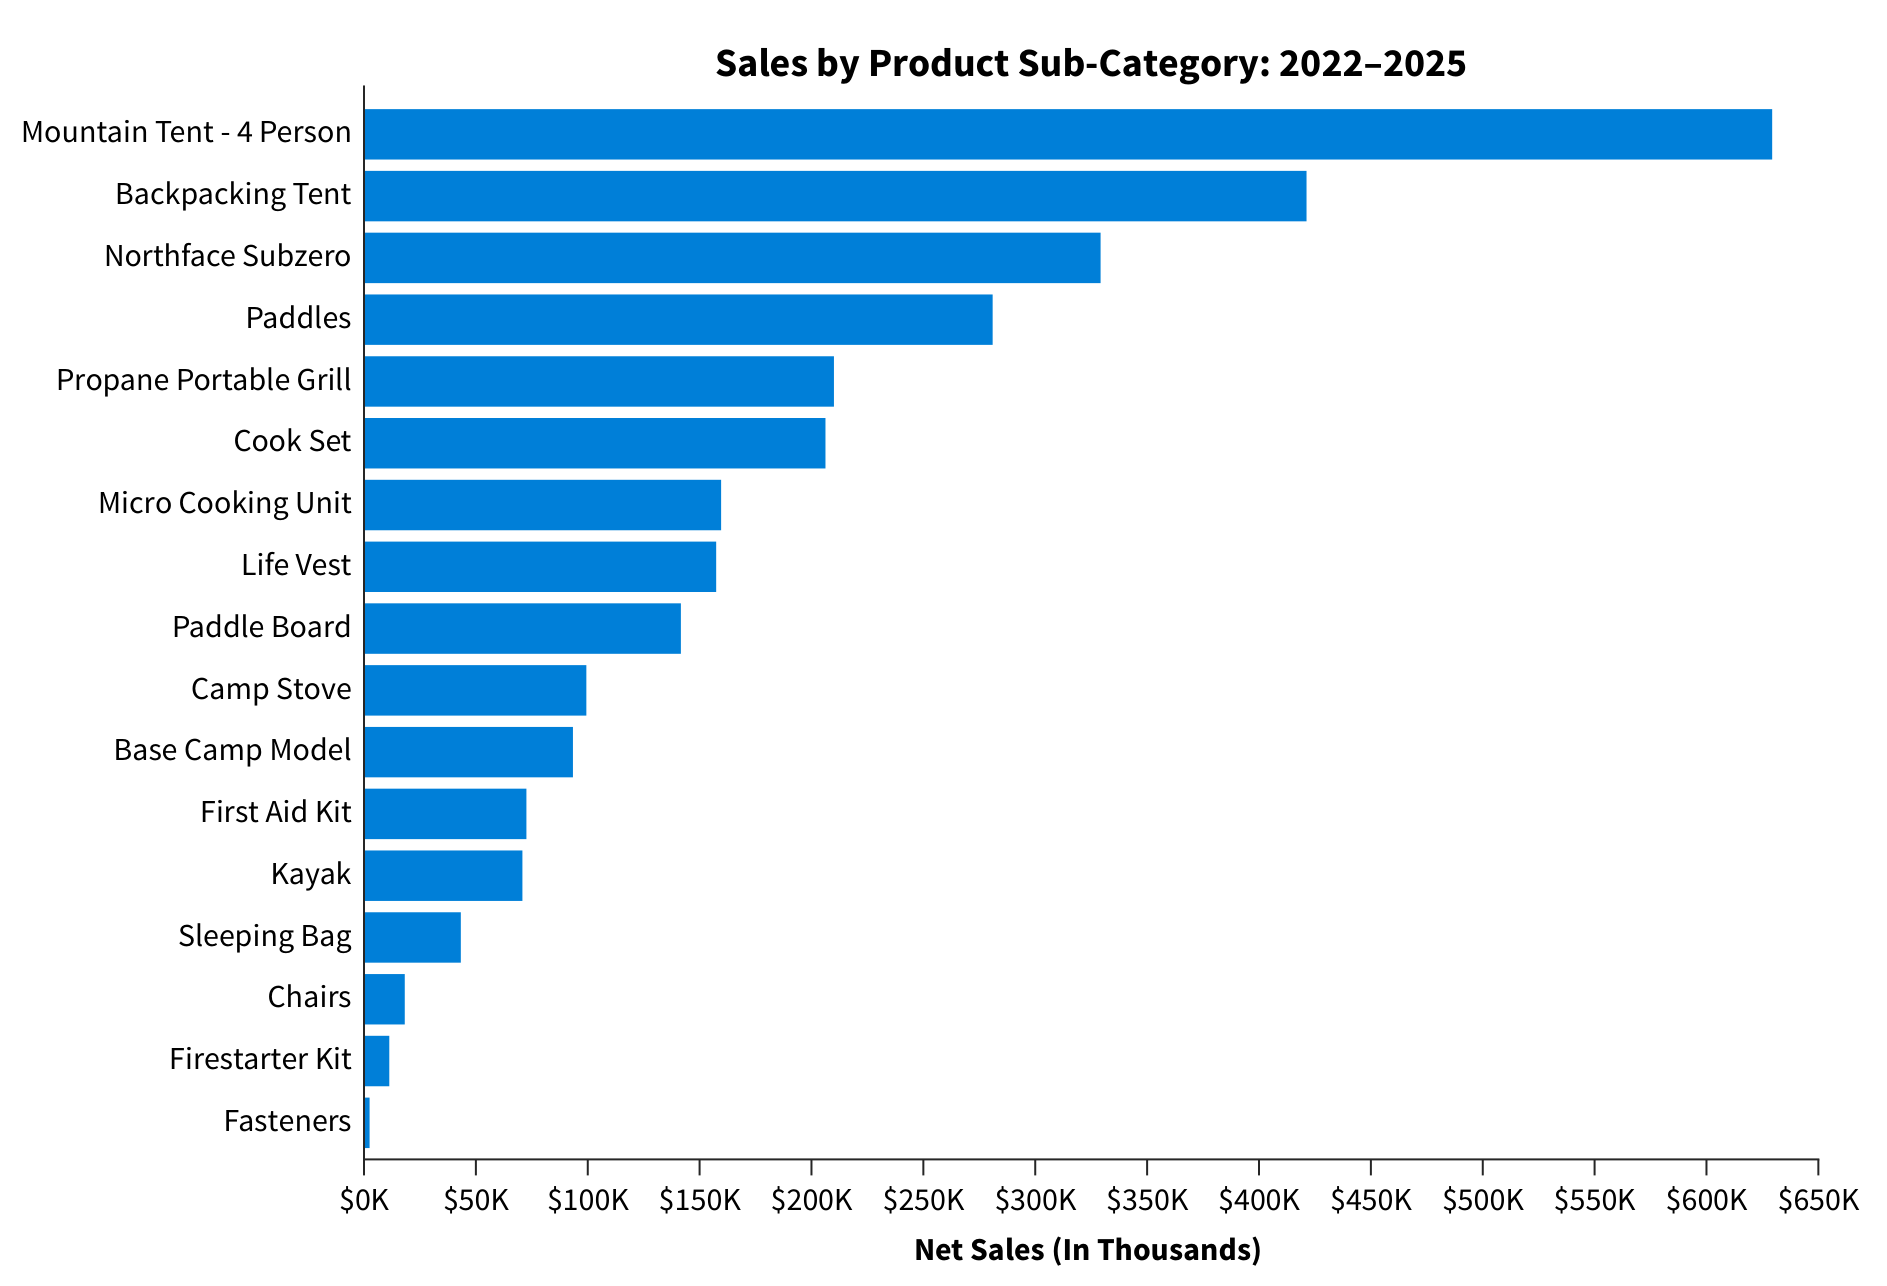
\includegraphics[width=0.95\textwidth,height=0.75\textheight,keepaspectratio]{../textbookForPractice/Figures/Ch_09/Apply It 9.3B.png}
    \end{figure}
\end{frame}

\begin{frame}{Madison public library 9.3}

    \begin{figure}[h]
        \centering
        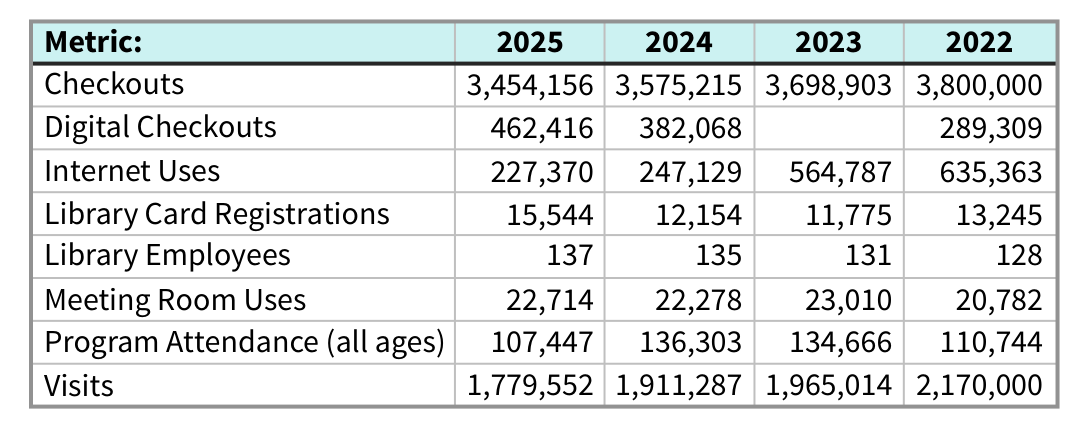
\includegraphics[width=0.95\textwidth,height=0.75\textheight,keepaspectratio]{../textbookForPractice/Figures/Ch_09/Madison public library 9.3.png}
    \end{figure}
\end{frame}

\begin{frame}{Apply It 9.4A}

    \begin{figure}[h]
        \centering
        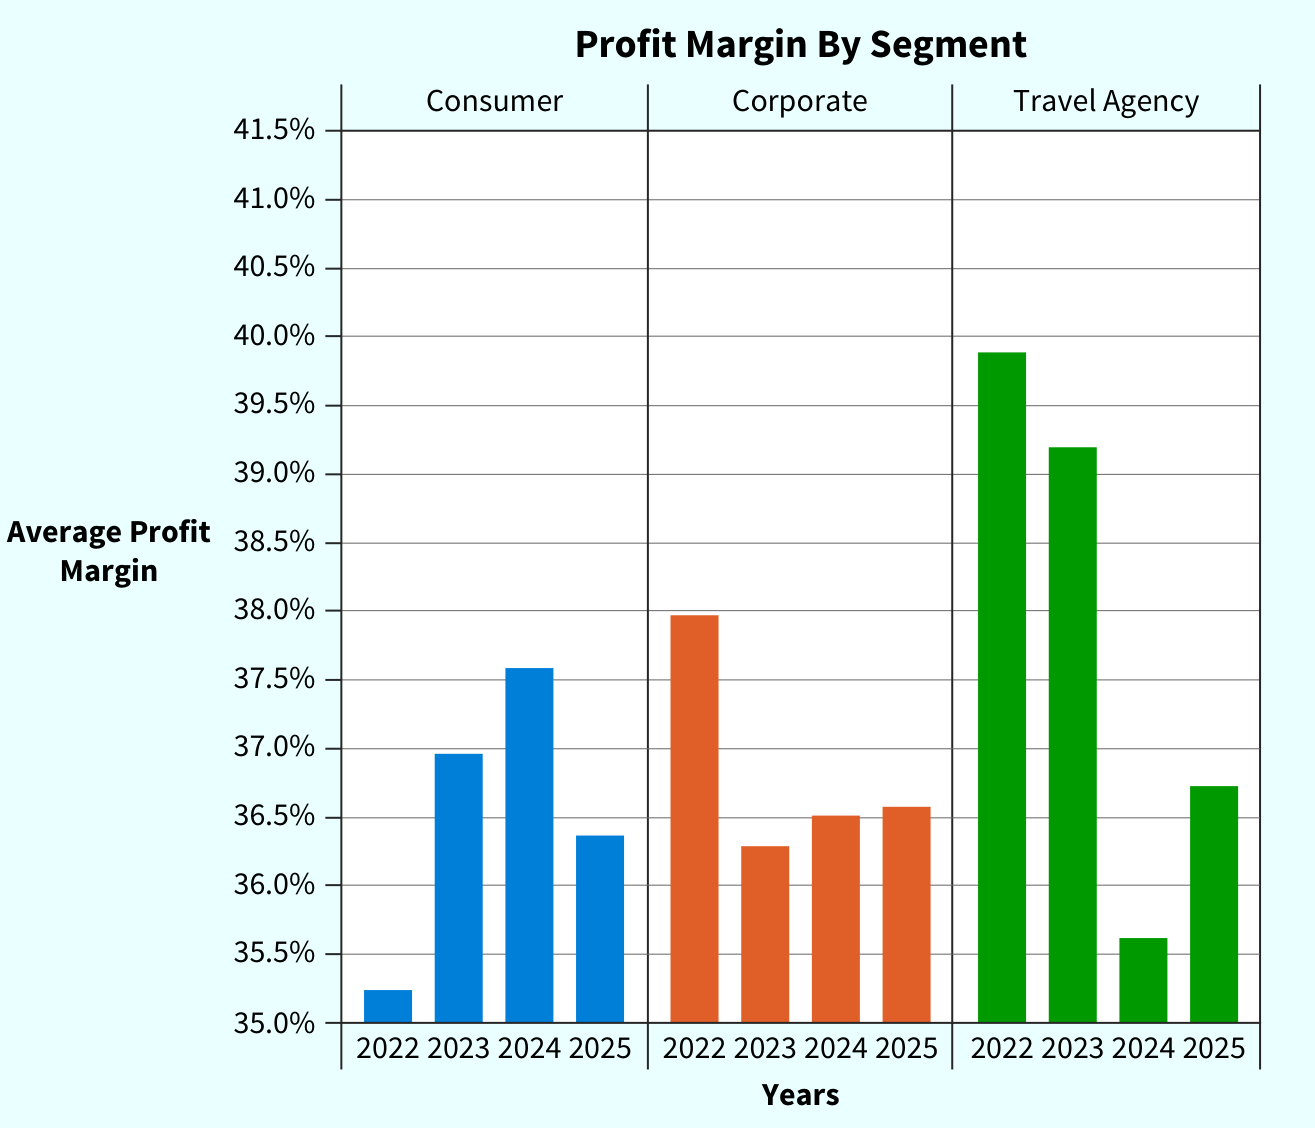
\includegraphics[width=0.95\textwidth,height=0.75\textheight,keepaspectratio]{../textbookForPractice/Figures/Ch_09/Apply It 9.4A.png}
    \end{figure}
\end{frame}

\begin{frame}{Apply It 9.4B}

    \begin{figure}[h]
        \centering
        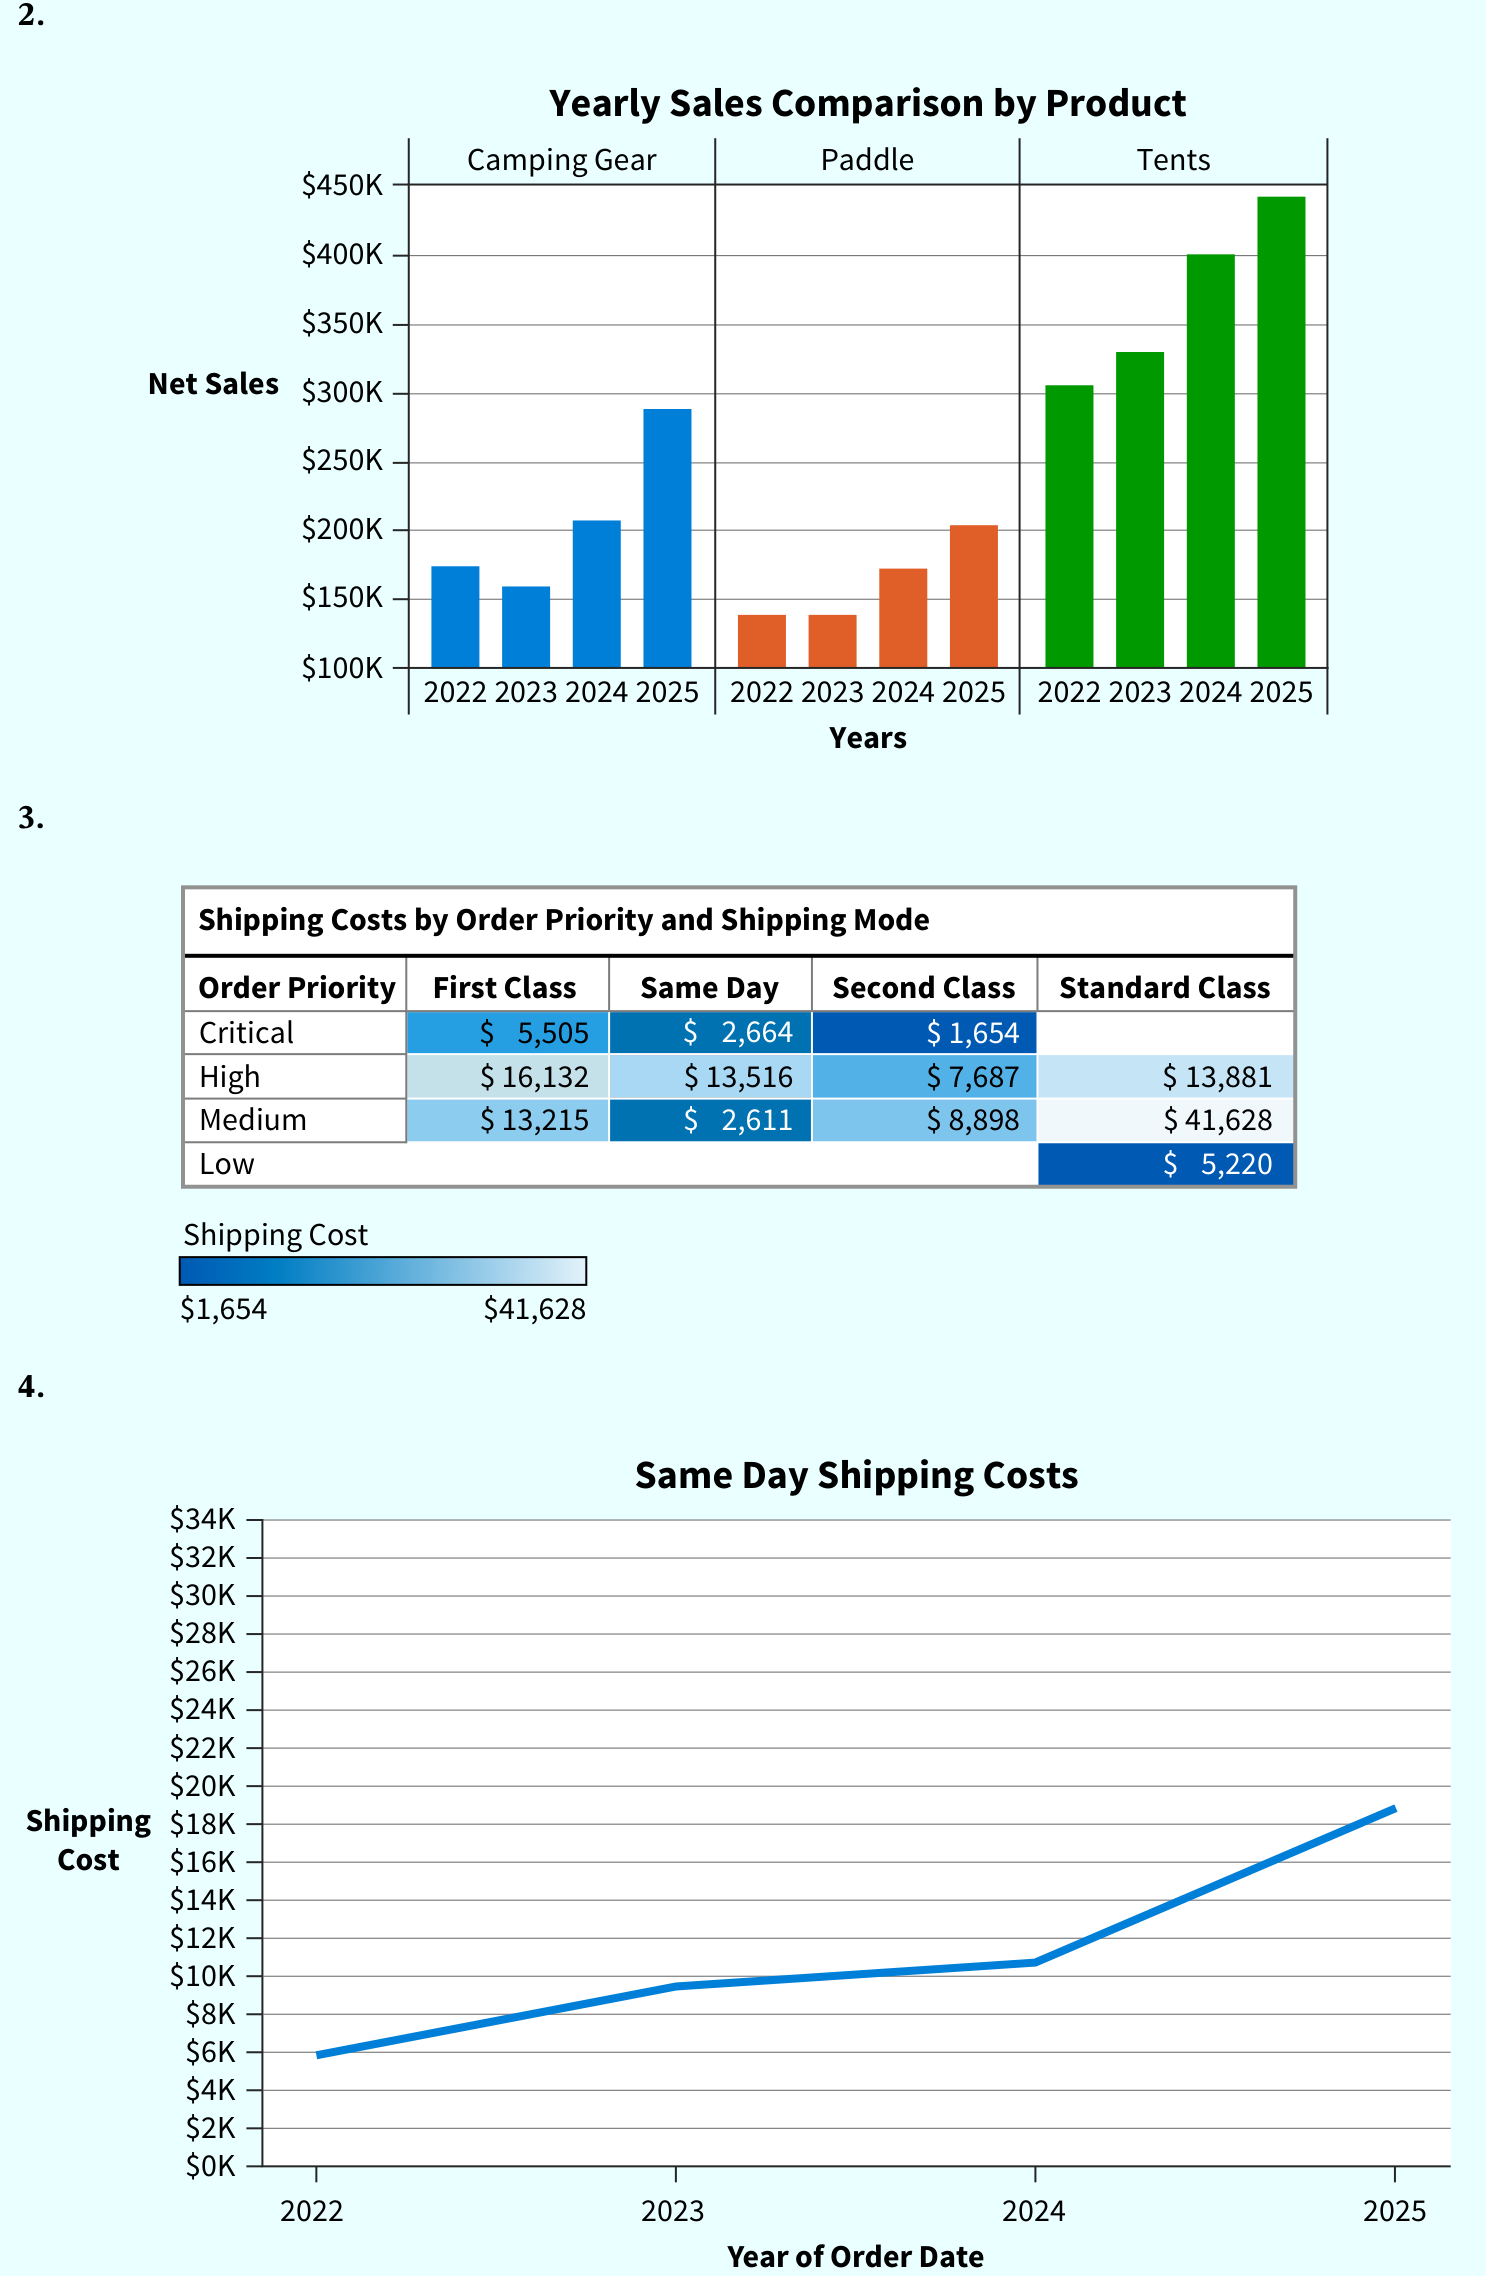
\includegraphics[width=0.95\textwidth,height=0.75\textheight,keepaspectratio]{../textbookForPractice/Figures/Ch_09/Apply It 9.4B.png}
    \end{figure}
\end{frame}

\begin{frame}{Apply It 9.4C}

    \begin{figure}[h]
        \centering
        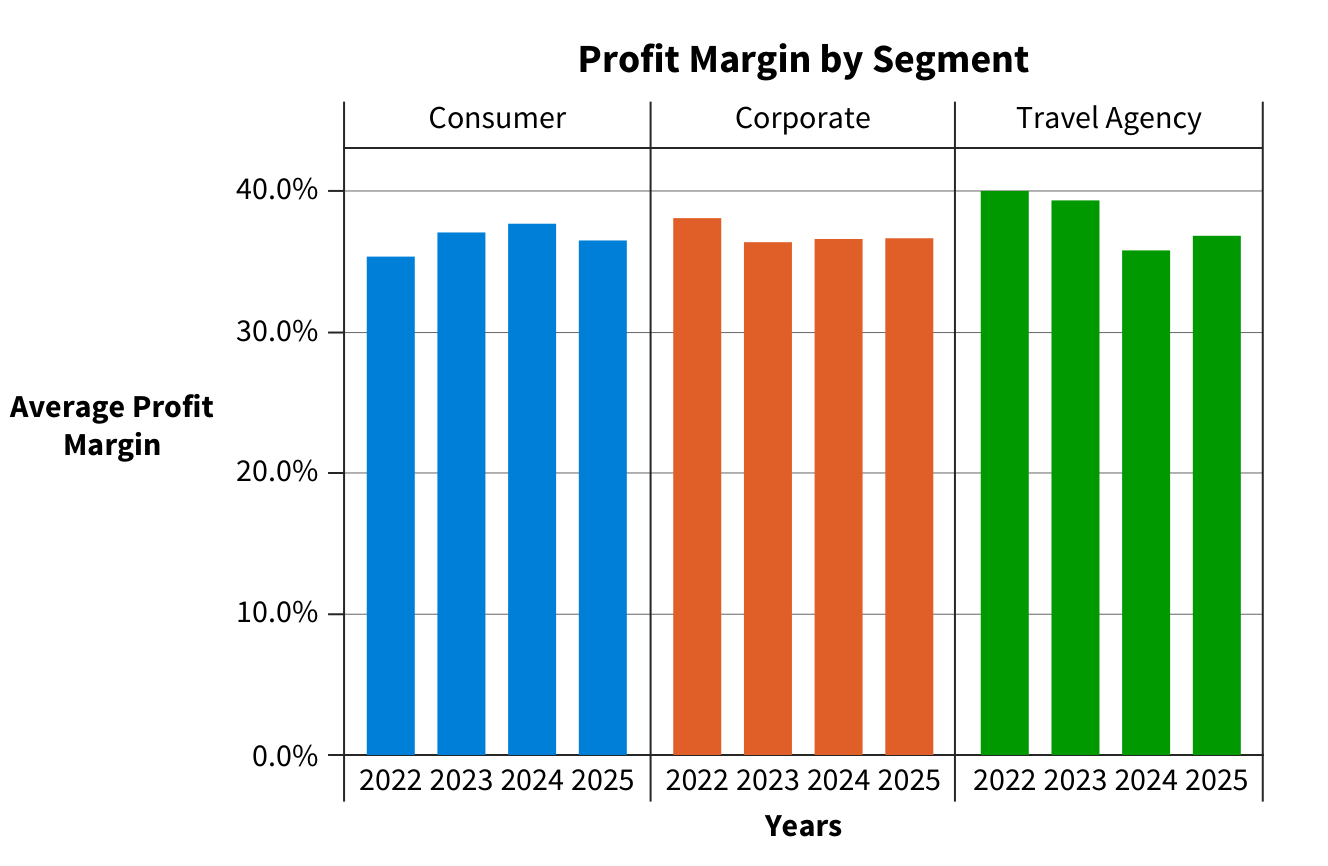
\includegraphics[width=0.95\textwidth,height=0.75\textheight,keepaspectratio]{../textbookForPractice/Figures/Ch_09/Apply It 9.4C.png}
    \end{figure}
\end{frame}

\begin{frame}{Apply It 9.4D}

    \begin{figure}[h]
        \centering
        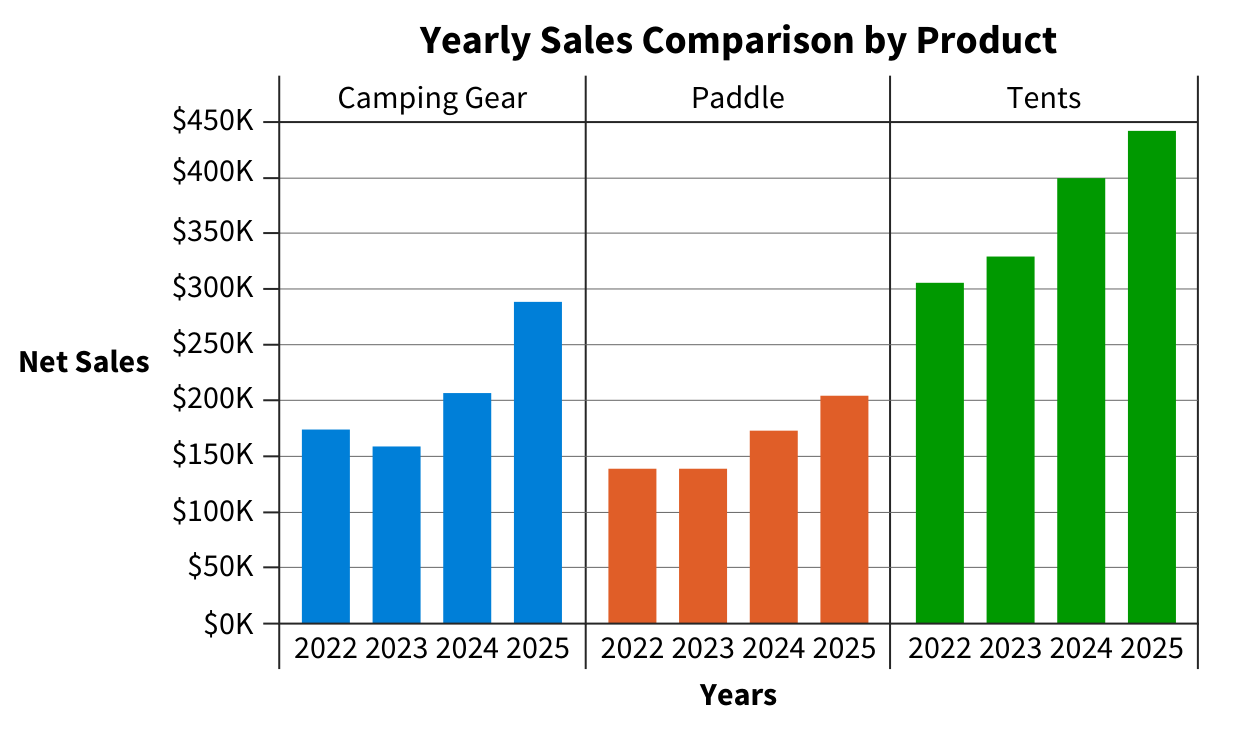
\includegraphics[width=0.95\textwidth,height=0.75\textheight,keepaspectratio]{../textbookForPractice/Figures/Ch_09/Apply It 9.4D.png}
    \end{figure}
\end{frame}

\begin{frame}{Apply It 9.4E}

    \begin{figure}[h]
        \centering
        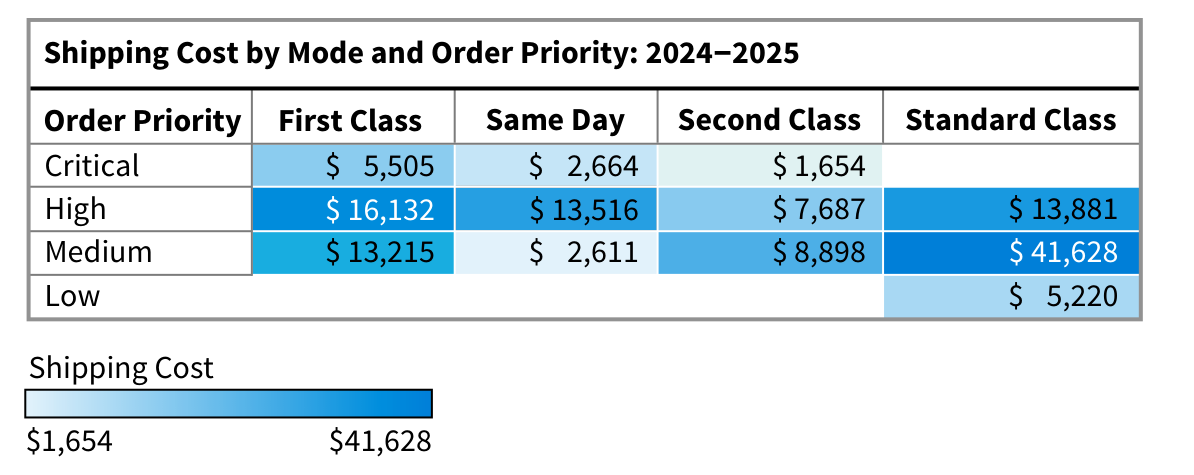
\includegraphics[width=0.95\textwidth,height=0.75\textheight,keepaspectratio]{../textbookForPractice/Figures/Ch_09/Apply It 9.4E.png}
    \end{figure}
\end{frame}

\begin{frame}{Apply It 9.4F}

    \begin{figure}[h]
        \centering
        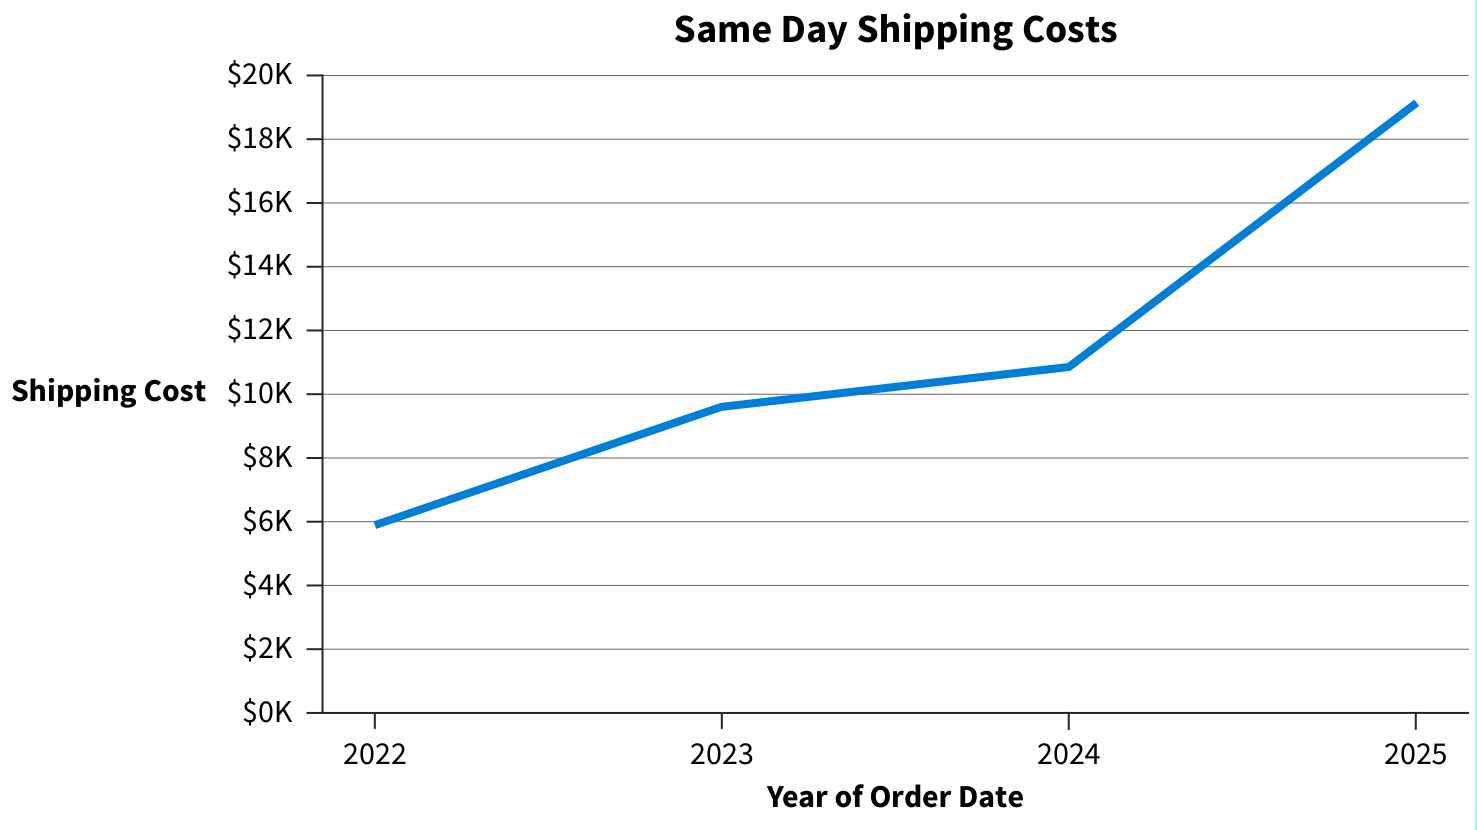
\includegraphics[width=0.95\textwidth,height=0.75\textheight,keepaspectratio]{../textbookForPractice/Figures/Ch_09/Apply It 9.4F.png}
    \end{figure}
\end{frame}

\begin{frame}{Apply It 9.5A}

    \begin{figure}[h]
        \centering
        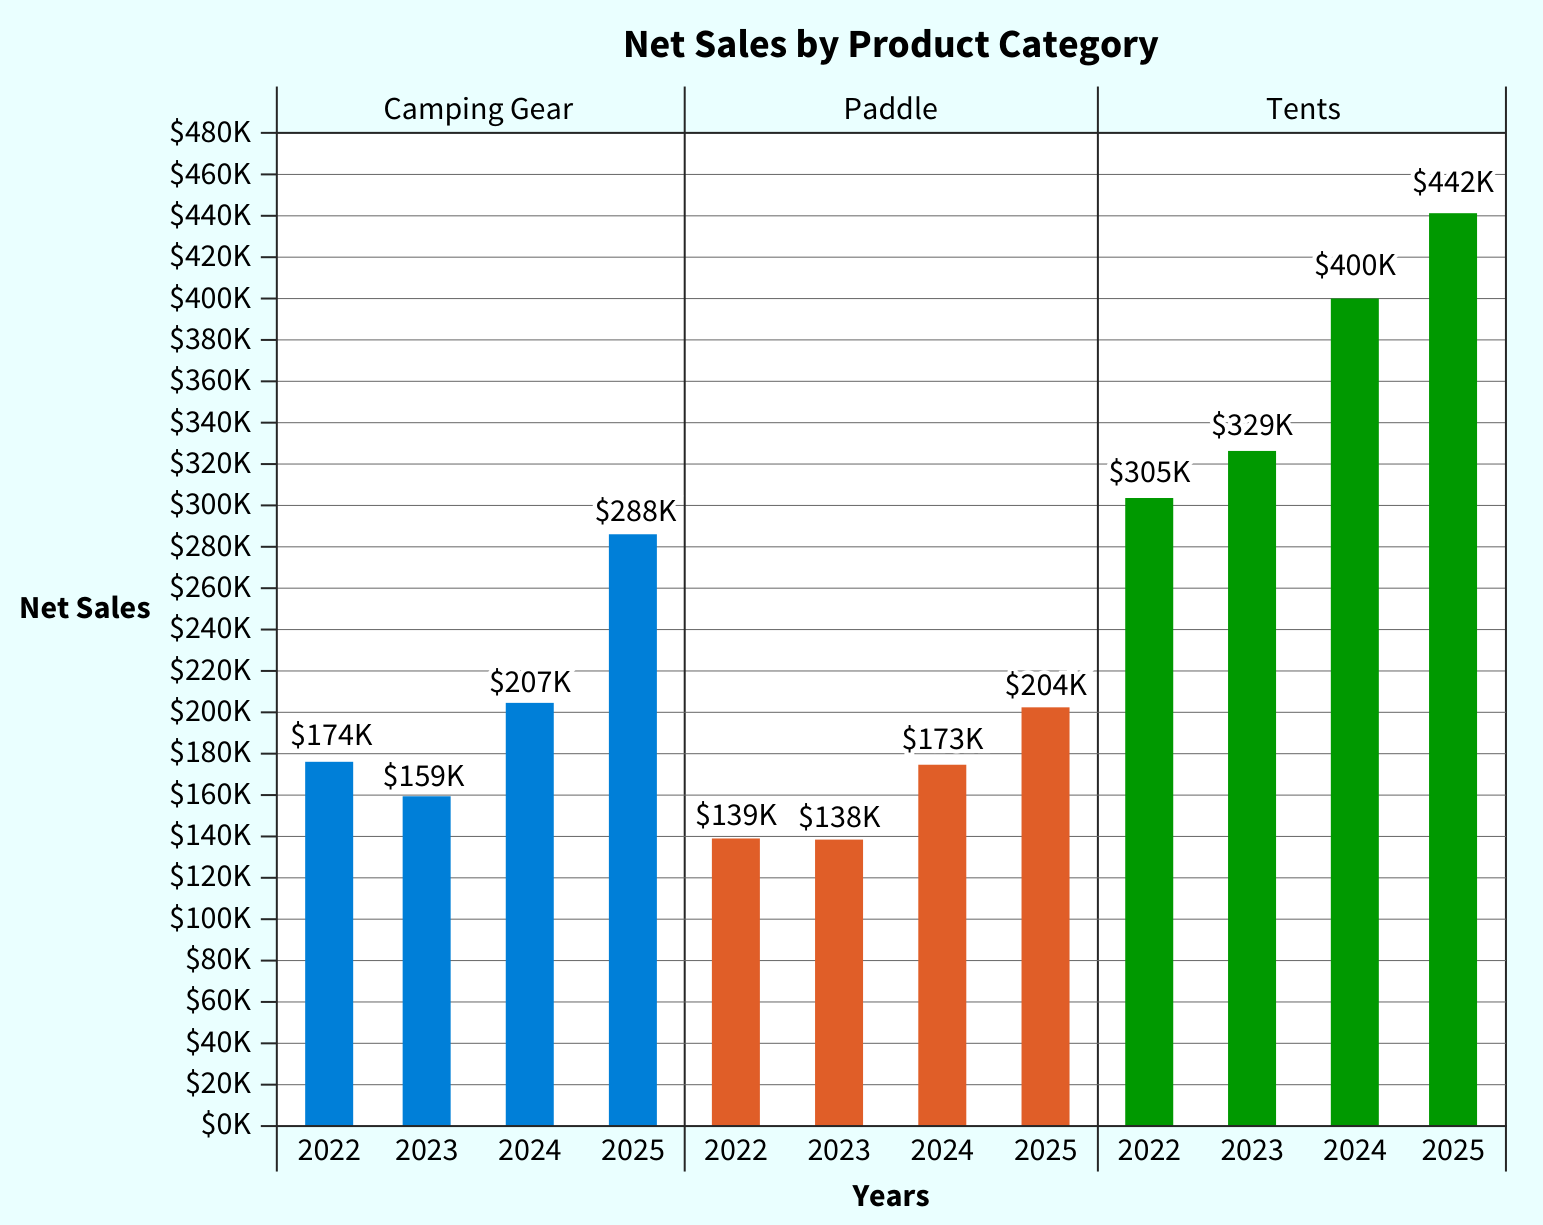
\includegraphics[width=0.95\textwidth,height=0.75\textheight,keepaspectratio]{../textbookForPractice/Figures/Ch_09/Apply It 9.5A.png}
    \end{figure}
\end{frame}

\begin{frame}{Apply It 9.5B}

    \begin{figure}[h]
        \centering
        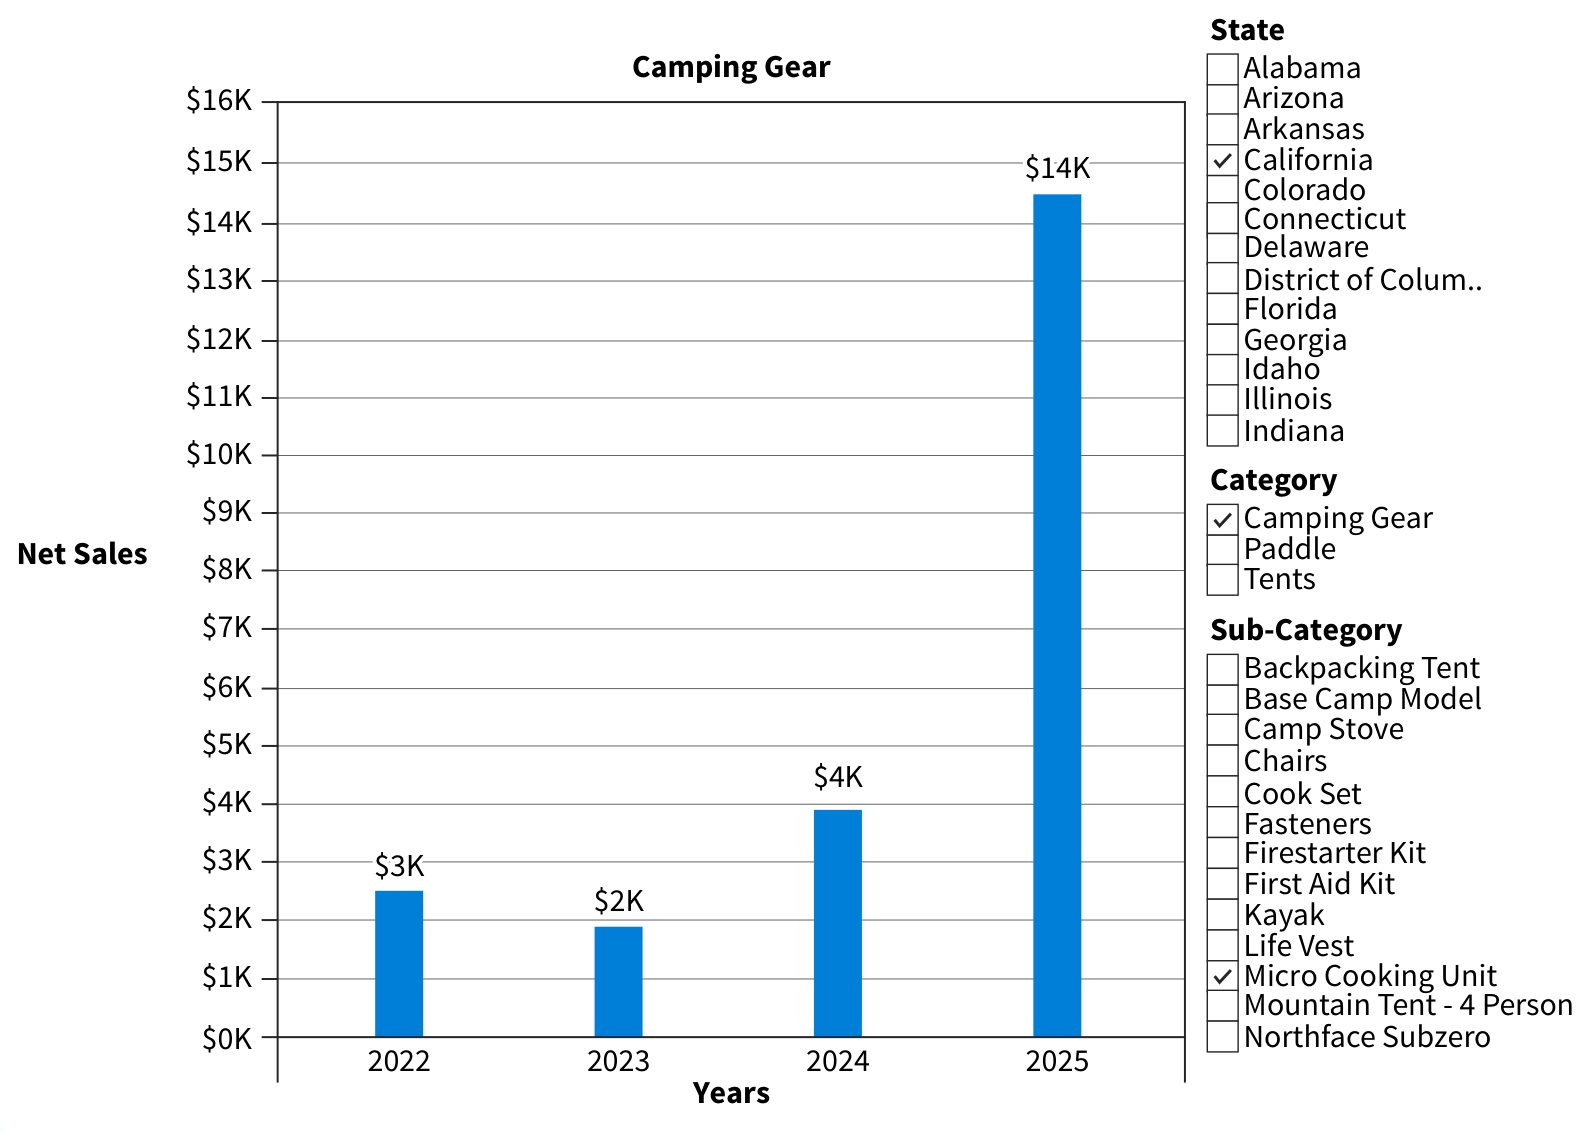
\includegraphics[width=0.95\textwidth,height=0.75\textheight,keepaspectratio]{../textbookForPractice/Figures/Ch_09/Apply It 9.5B.png}
    \end{figure}
\end{frame}

\begin{frame}{Bài tập Ngắn (Brief Exercises)}
\begin{center}
            \Huge \textbf{Phần Bài tập Ngắn} \\
            \vspace{0.5cm}
            \Large Brief Exercises (BE)
        \end{center}
\end{frame}

\begin{frame}{BE 9.8 \& BE 9.9}
    \begin{columns}
        \begin{column}{0.5\textwidth}
            \begin{figure}[h]
                \centering
                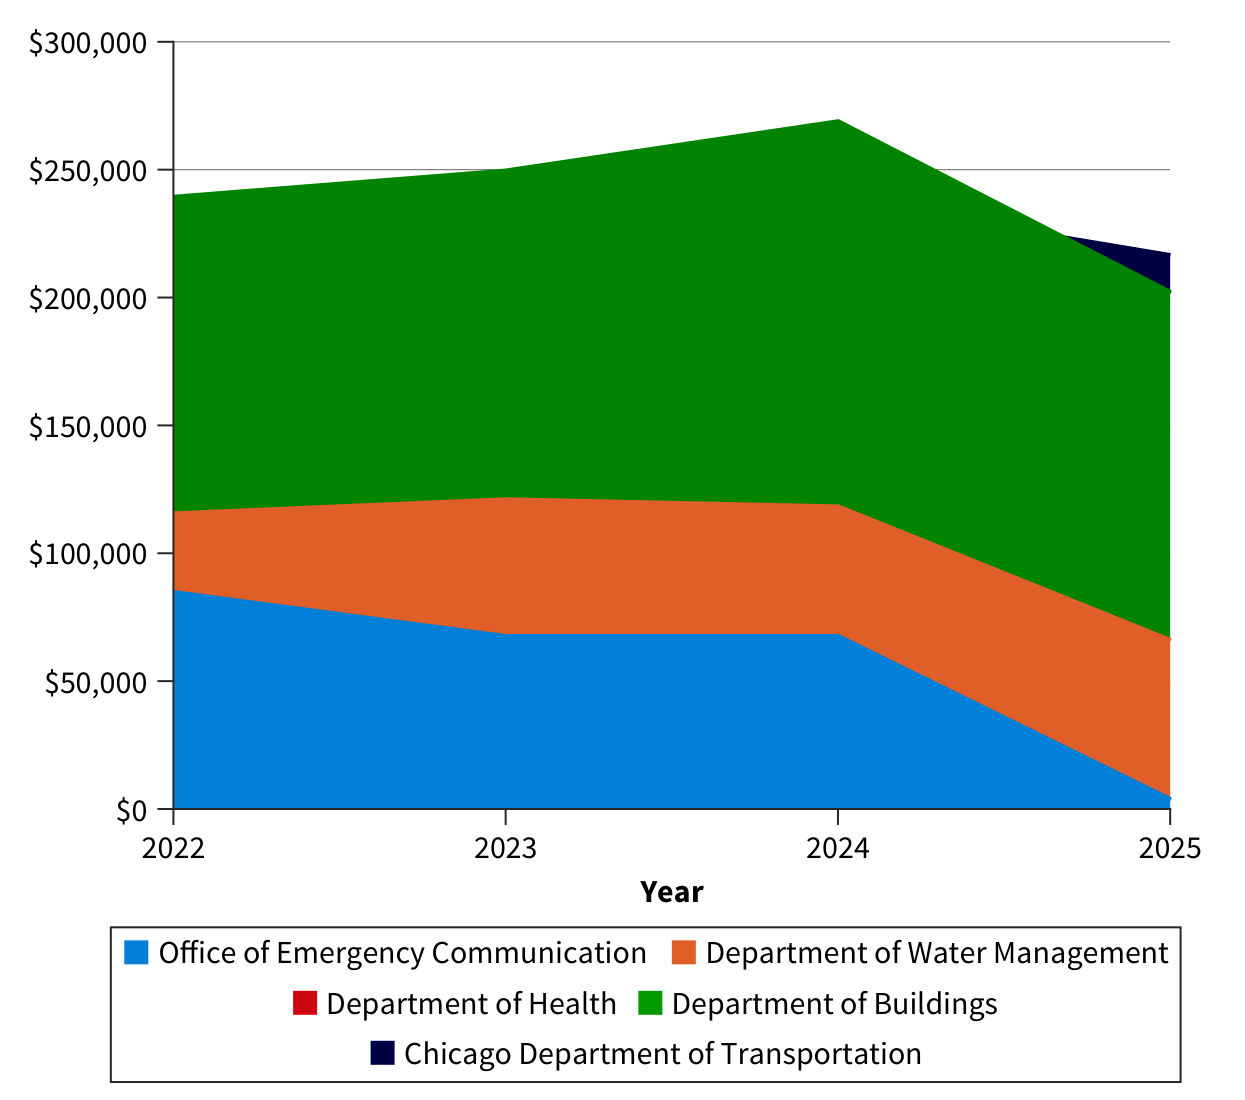
\includegraphics[width=\textwidth,height=0.7\textheight,keepaspectratio]{../textbookForPractice/Figures/Ch_09/BE 9.8.png}
            \end{figure}
        \end{column}
        \begin{column}{0.5\textwidth}
            \begin{figure}[h]
                \centering
                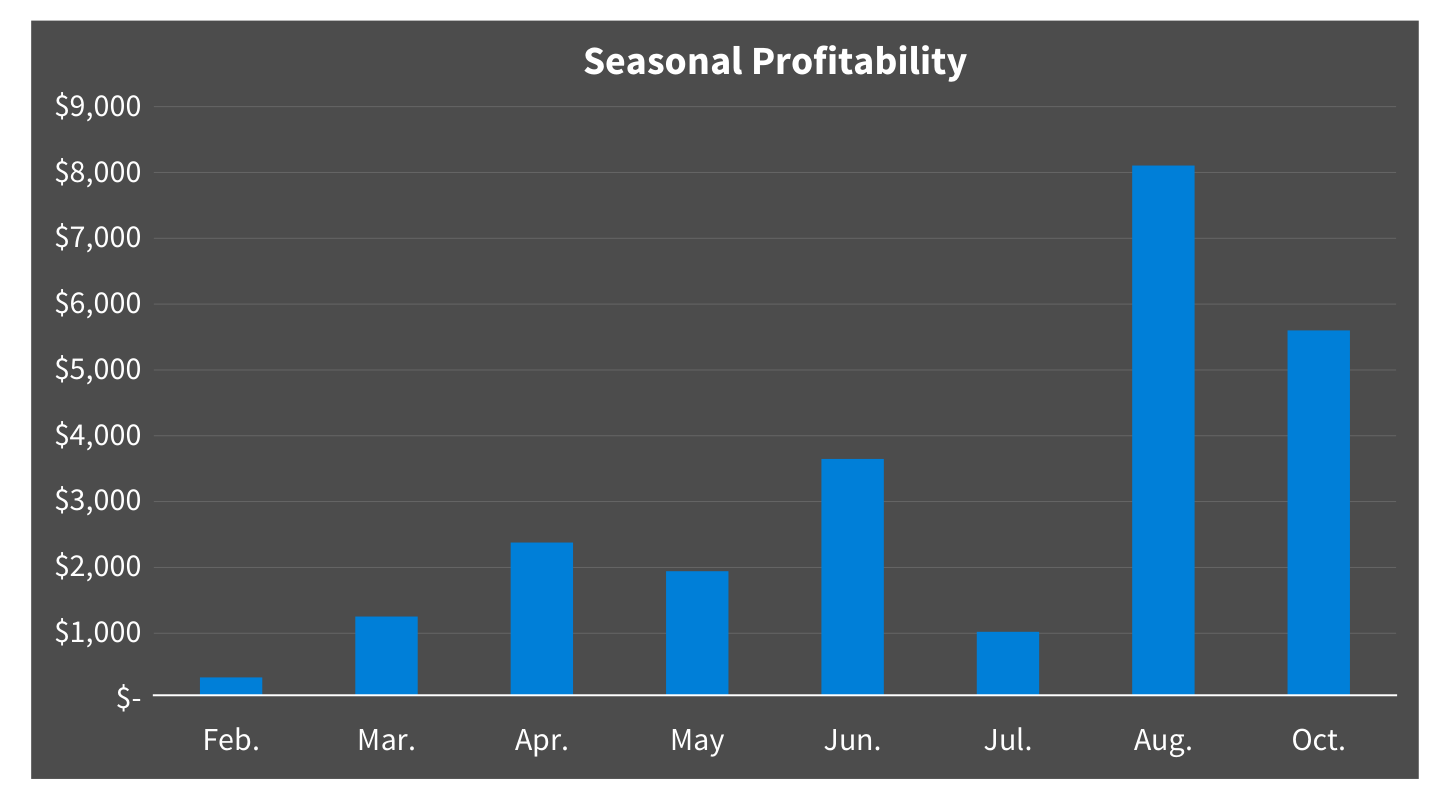
\includegraphics[width=\textwidth,height=0.7\textheight,keepaspectratio]{../textbookForPractice/Figures/Ch_09/BE 9.9.png}
            \end{figure}
        \end{column}
    \end{columns}
\end{frame}

\begin{frame}{BE 9.10 \& BE 9.11}
    \begin{columns}
        \begin{column}{0.5\textwidth}
            \begin{figure}[h]
                \centering
                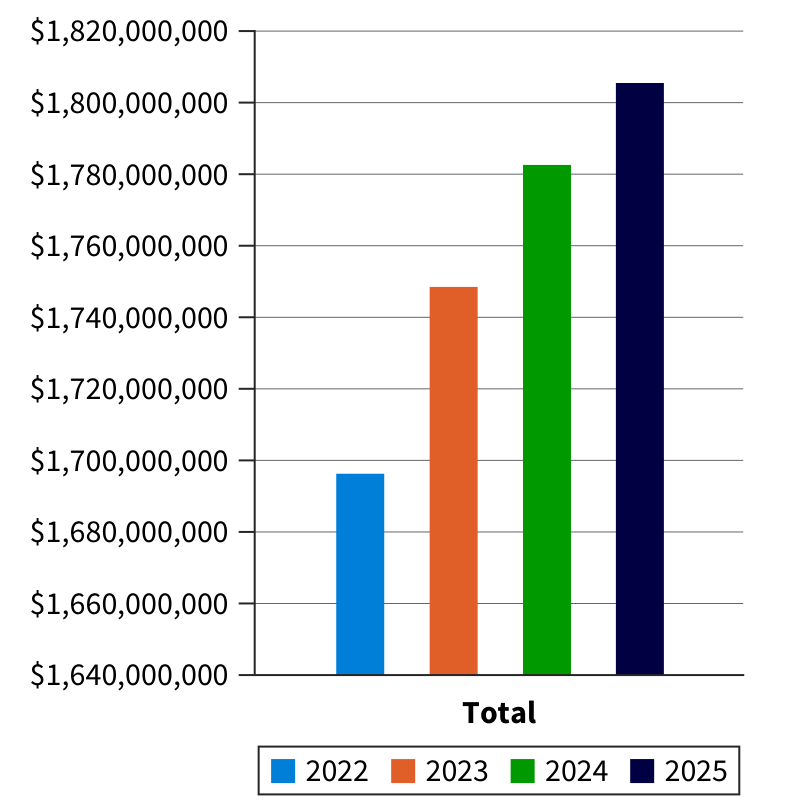
\includegraphics[width=\textwidth,height=0.7\textheight,keepaspectratio]{../textbookForPractice/Figures/Ch_09/BE 9.10.png}
            \end{figure}
        \end{column}
        \begin{column}{0.5\textwidth}
            \begin{figure}[h]
                \centering
                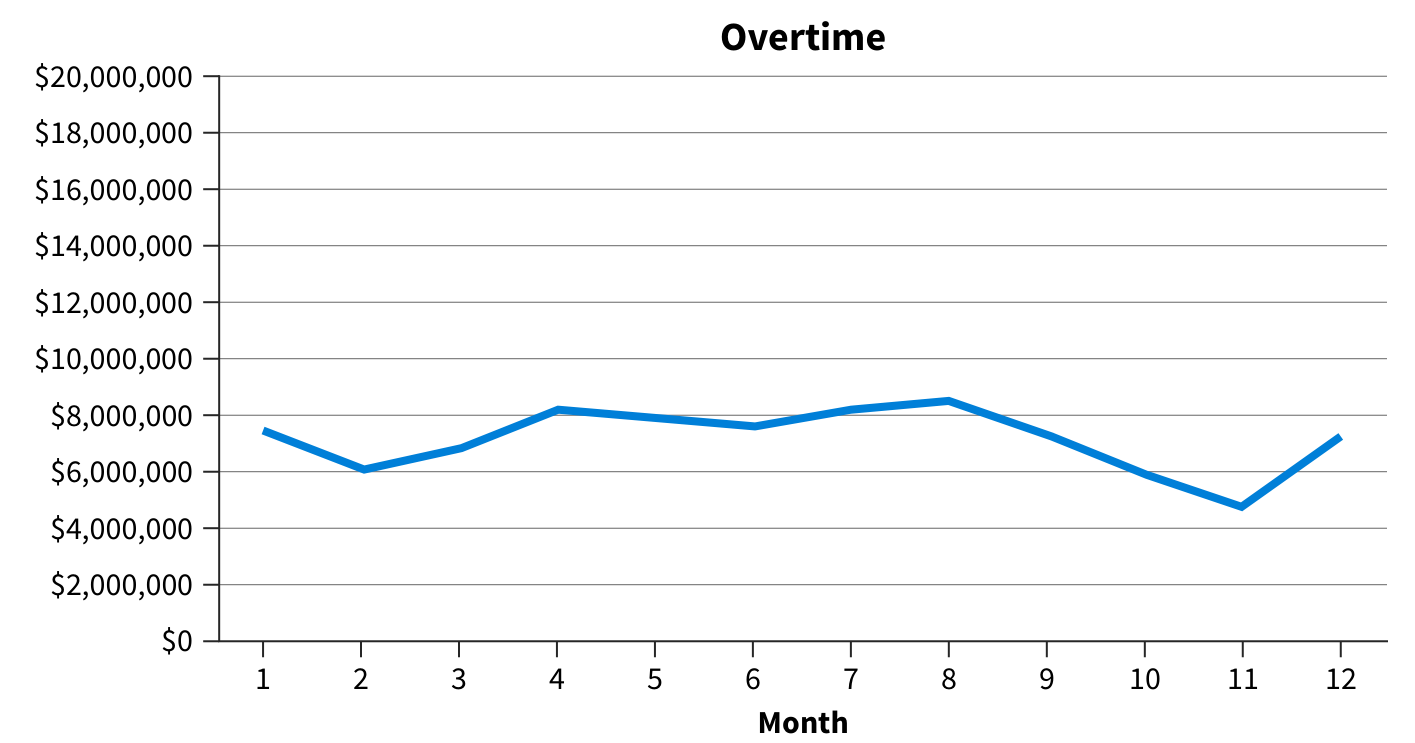
\includegraphics[width=\textwidth,height=0.7\textheight,keepaspectratio]{../textbookForPractice/Figures/Ch_09/BE 9.11.png}
            \end{figure}
        \end{column}
    \end{columns}
\end{frame}

\begin{frame}{BE 9.12 \& BE 9.13}
    \begin{columns}
        \begin{column}{0.5\textwidth}
            \begin{figure}[h]
                \centering
                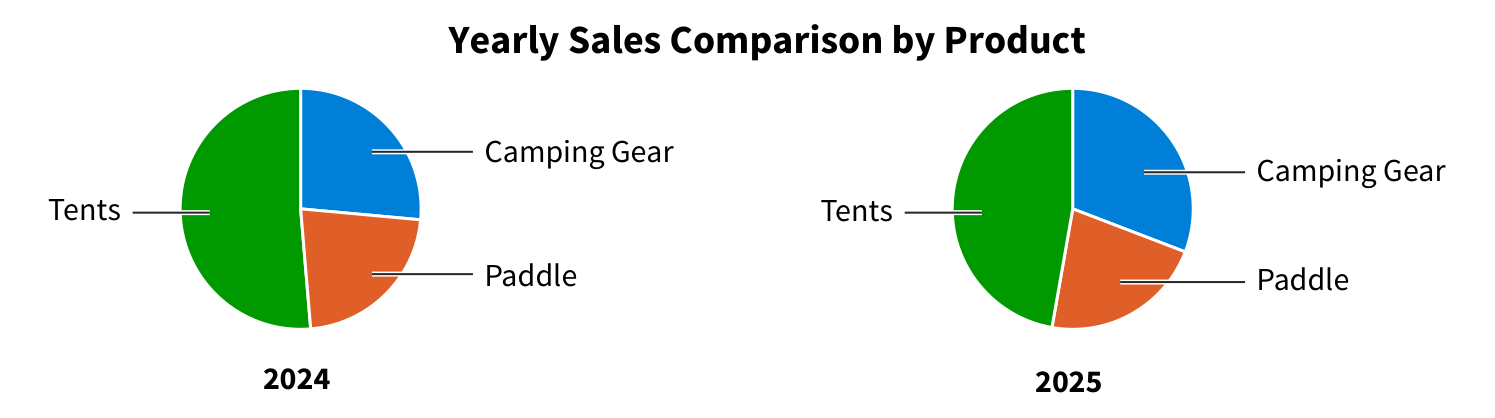
\includegraphics[width=\textwidth,height=0.7\textheight,keepaspectratio]{../textbookForPractice/Figures/Ch_09/BE 9.12.png}
            \end{figure}
        \end{column}
        \begin{column}{0.5\textwidth}
            \begin{figure}[h]
                \centering
                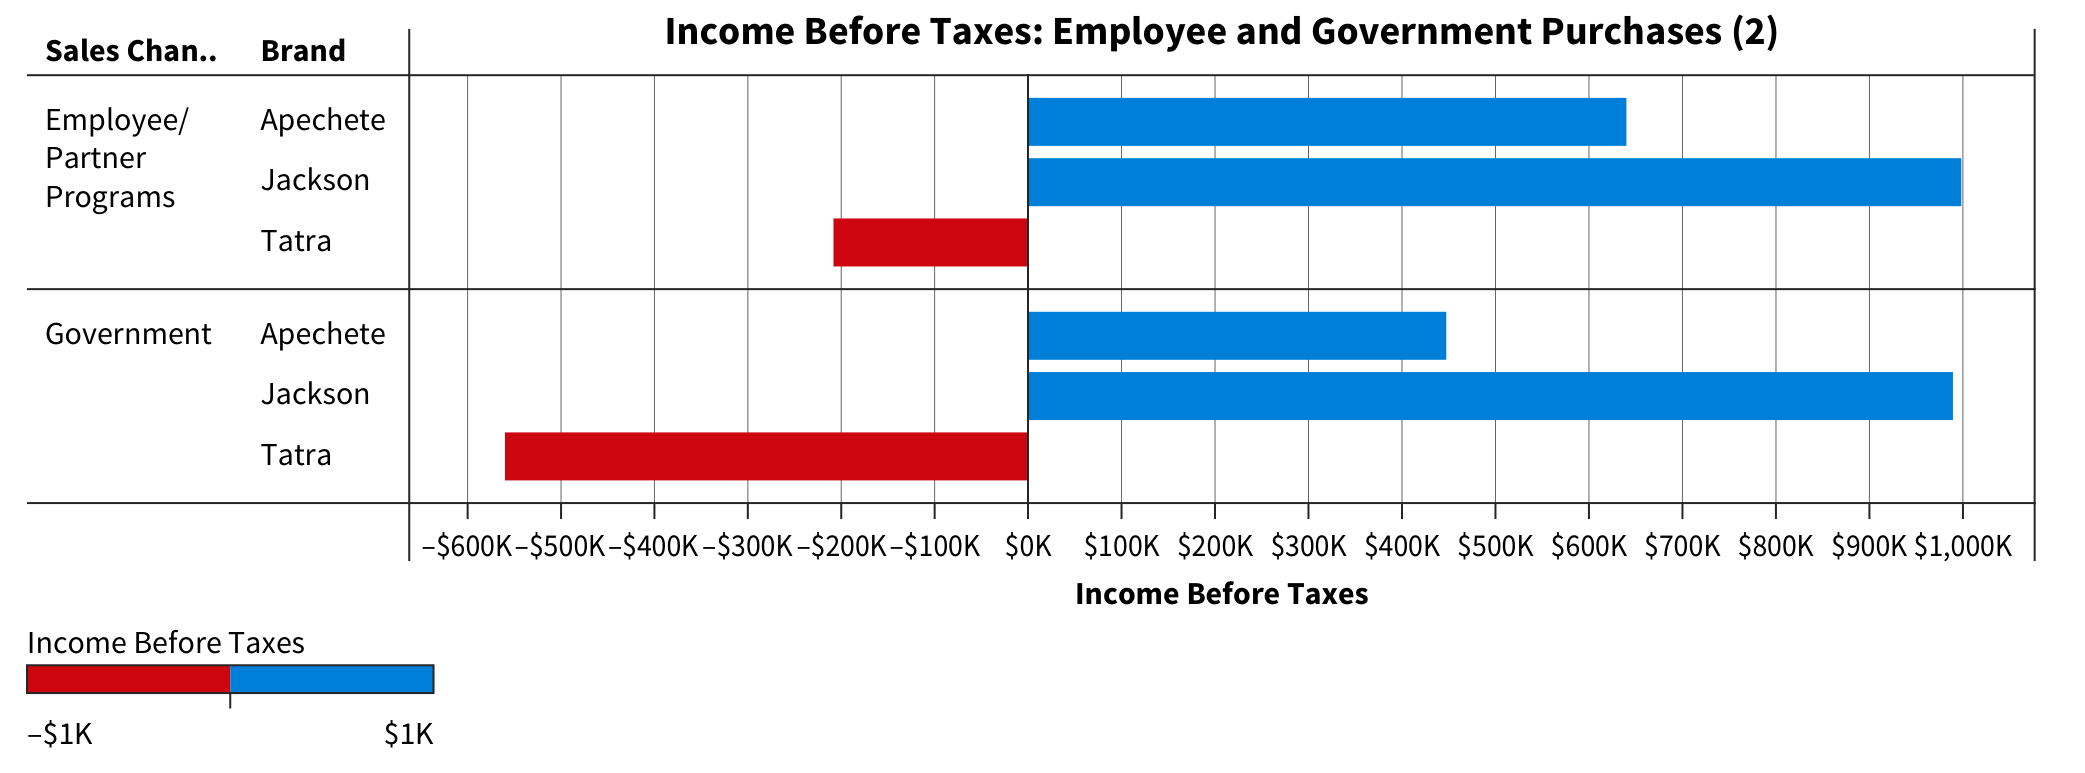
\includegraphics[width=\textwidth,height=0.7\textheight,keepaspectratio]{../textbookForPractice/Figures/Ch_09/BE 9.13.png}
            \end{figure}
        \end{column}
    \end{columns}
\end{frame}

\begin{frame}{BE 9.14 \& BE 9.15}
    \begin{columns}
        \begin{column}{0.5\textwidth}
            \begin{figure}[h]
                \centering
                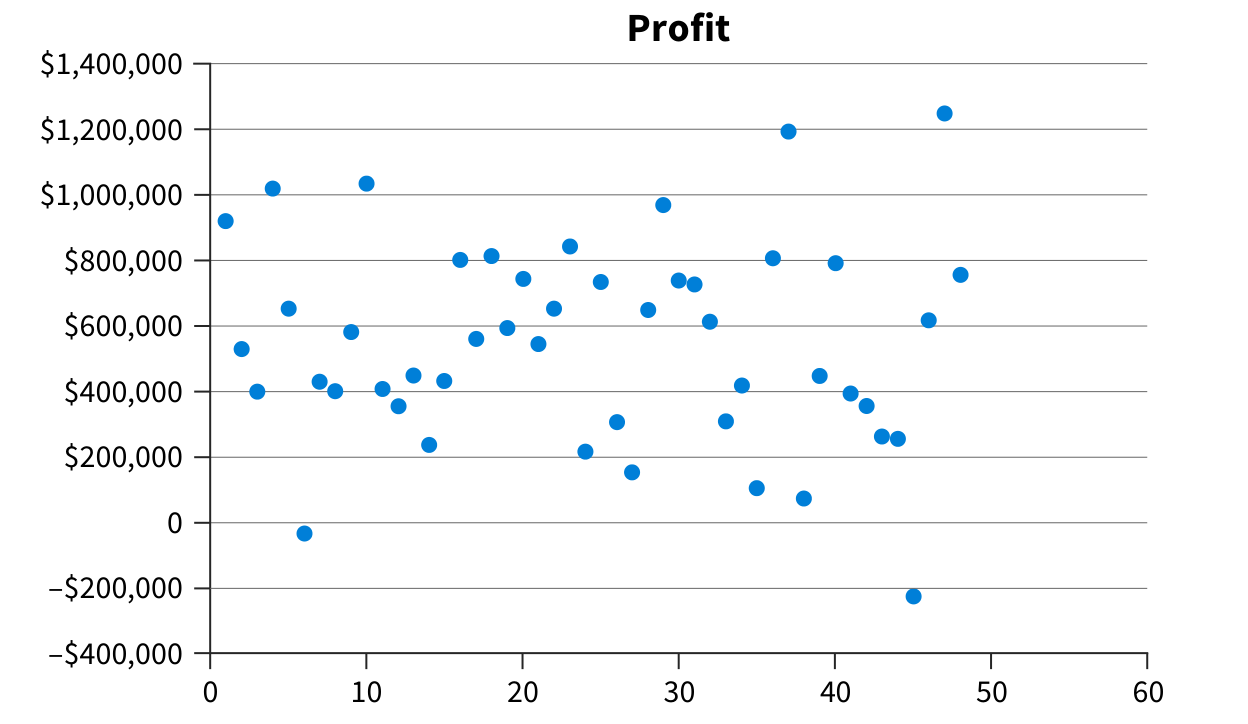
\includegraphics[width=\textwidth,height=0.7\textheight,keepaspectratio]{../textbookForPractice/Figures/Ch_09/BE 9.14.png}
            \end{figure}
        \end{column}
        \begin{column}{0.5\textwidth}
            \begin{figure}[h]
                \centering
                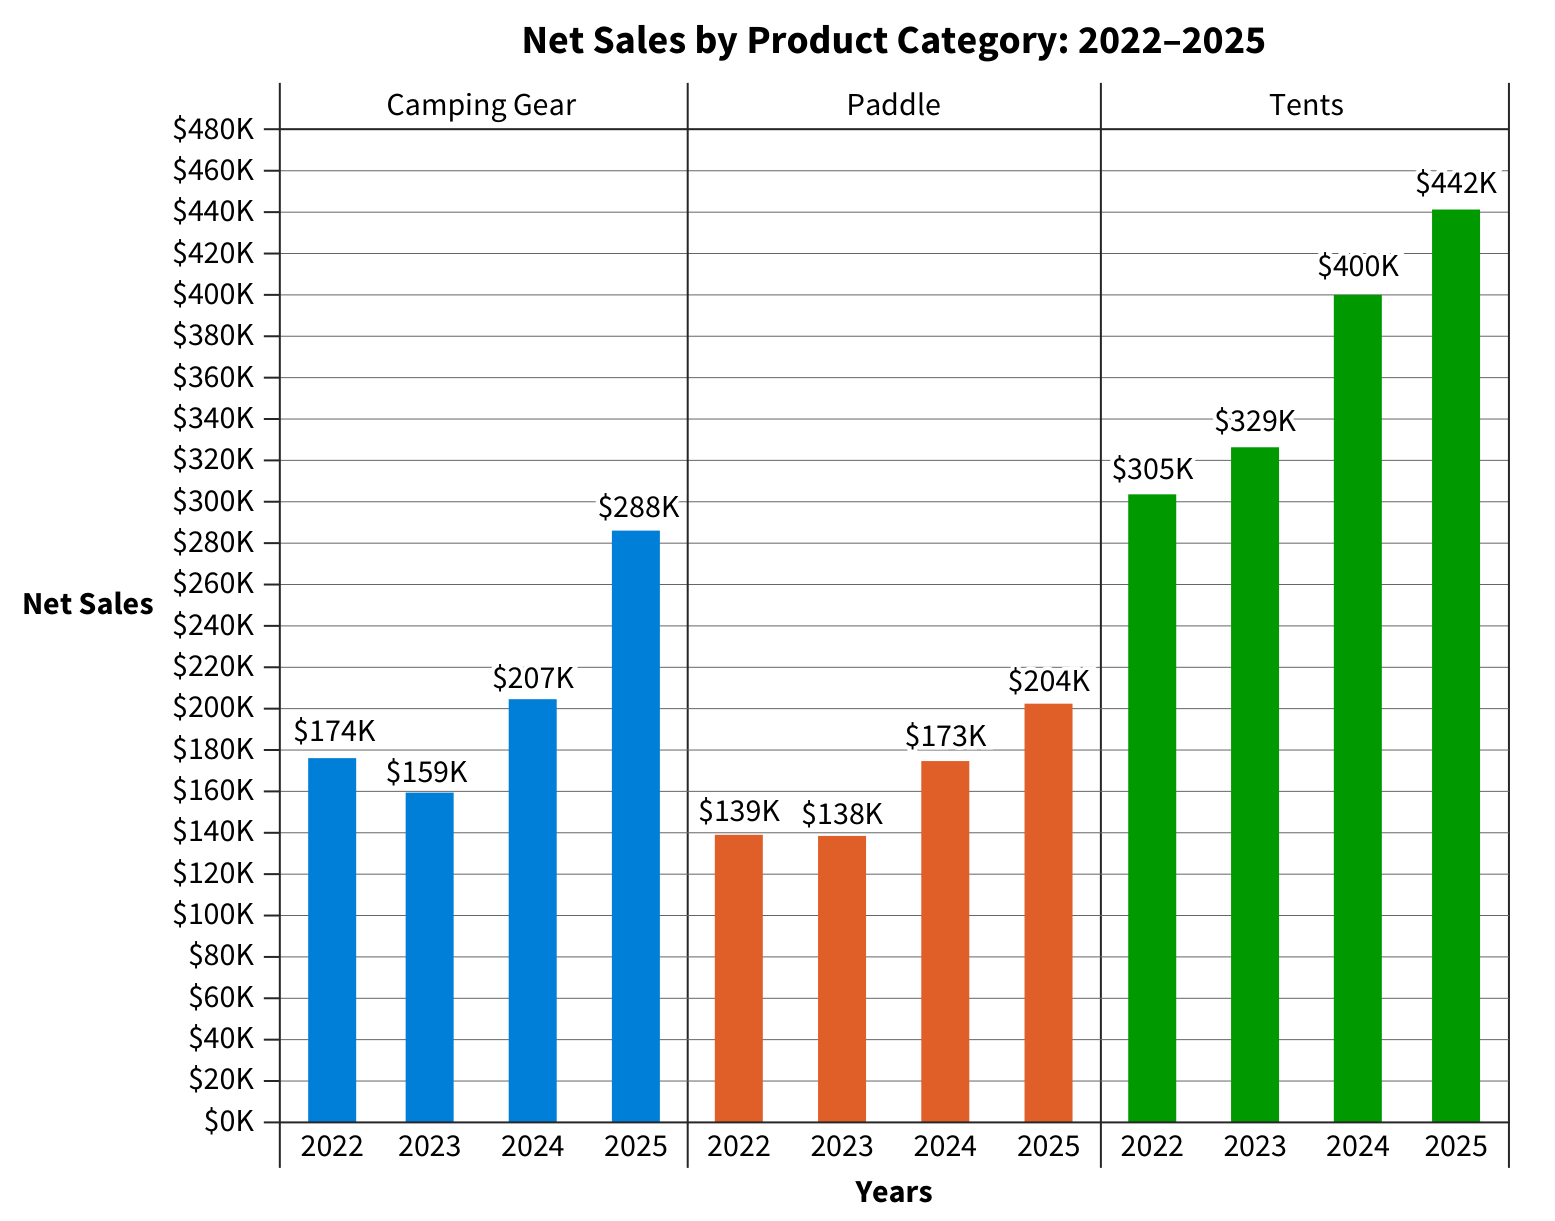
\includegraphics[width=\textwidth,height=0.7\textheight,keepaspectratio]{../textbookForPractice/Figures/Ch_09/BE 9.15.png}
            \end{figure}
        \end{column}
    \end{columns}
\end{frame}

\begin{frame}{Bài tập (Exercises)}
\begin{center}
            \Huge \textbf{Phần Bài tập} \\
            \vspace{0.5cm}
            \Large Exercises (EX)
        \end{center}
\end{frame}

\begin{frame}{EX 9.10 \& EX 9.11}
    \begin{columns}
        \begin{column}{0.5\textwidth}
            \begin{figure}[h]
                \centering
                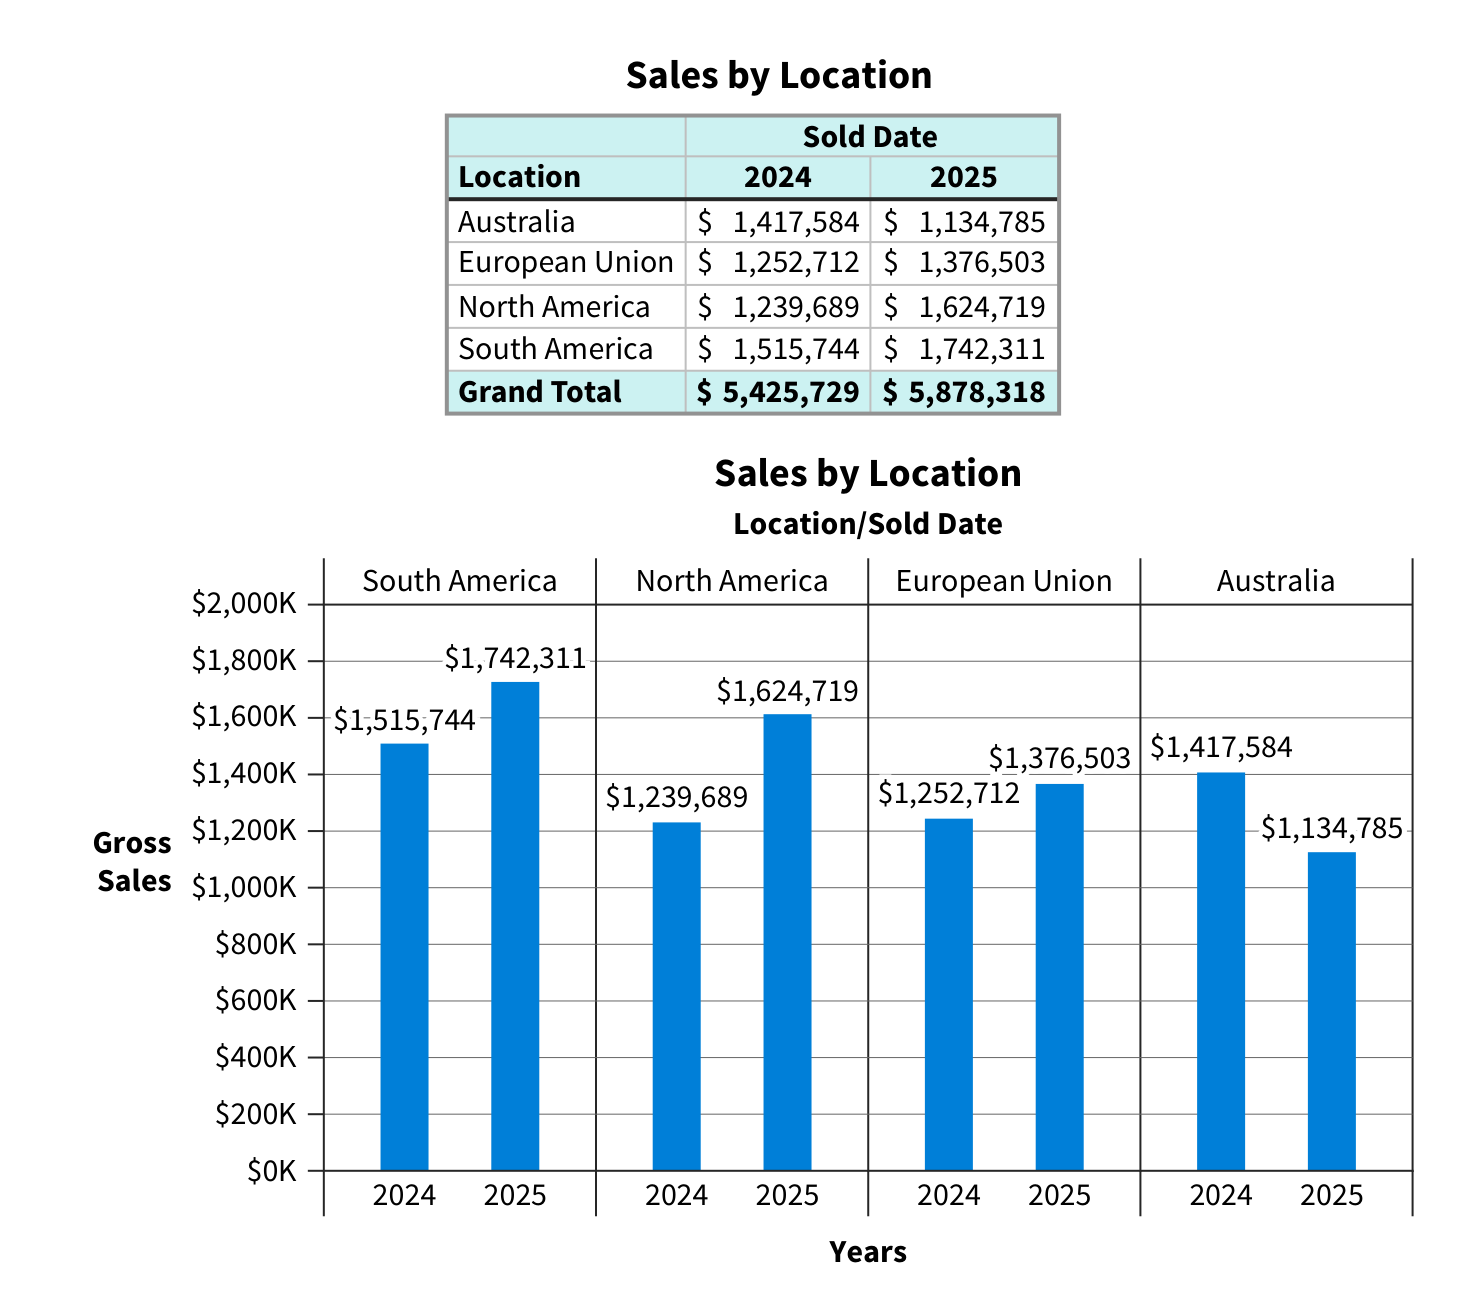
\includegraphics[width=\textwidth,height=0.7\textheight,keepaspectratio]{../textbookForPractice/Figures/Ch_09/EX 9.10.png}
            \end{figure}
        \end{column}
        \begin{column}{0.5\textwidth}
            \begin{figure}[h]
                \centering
                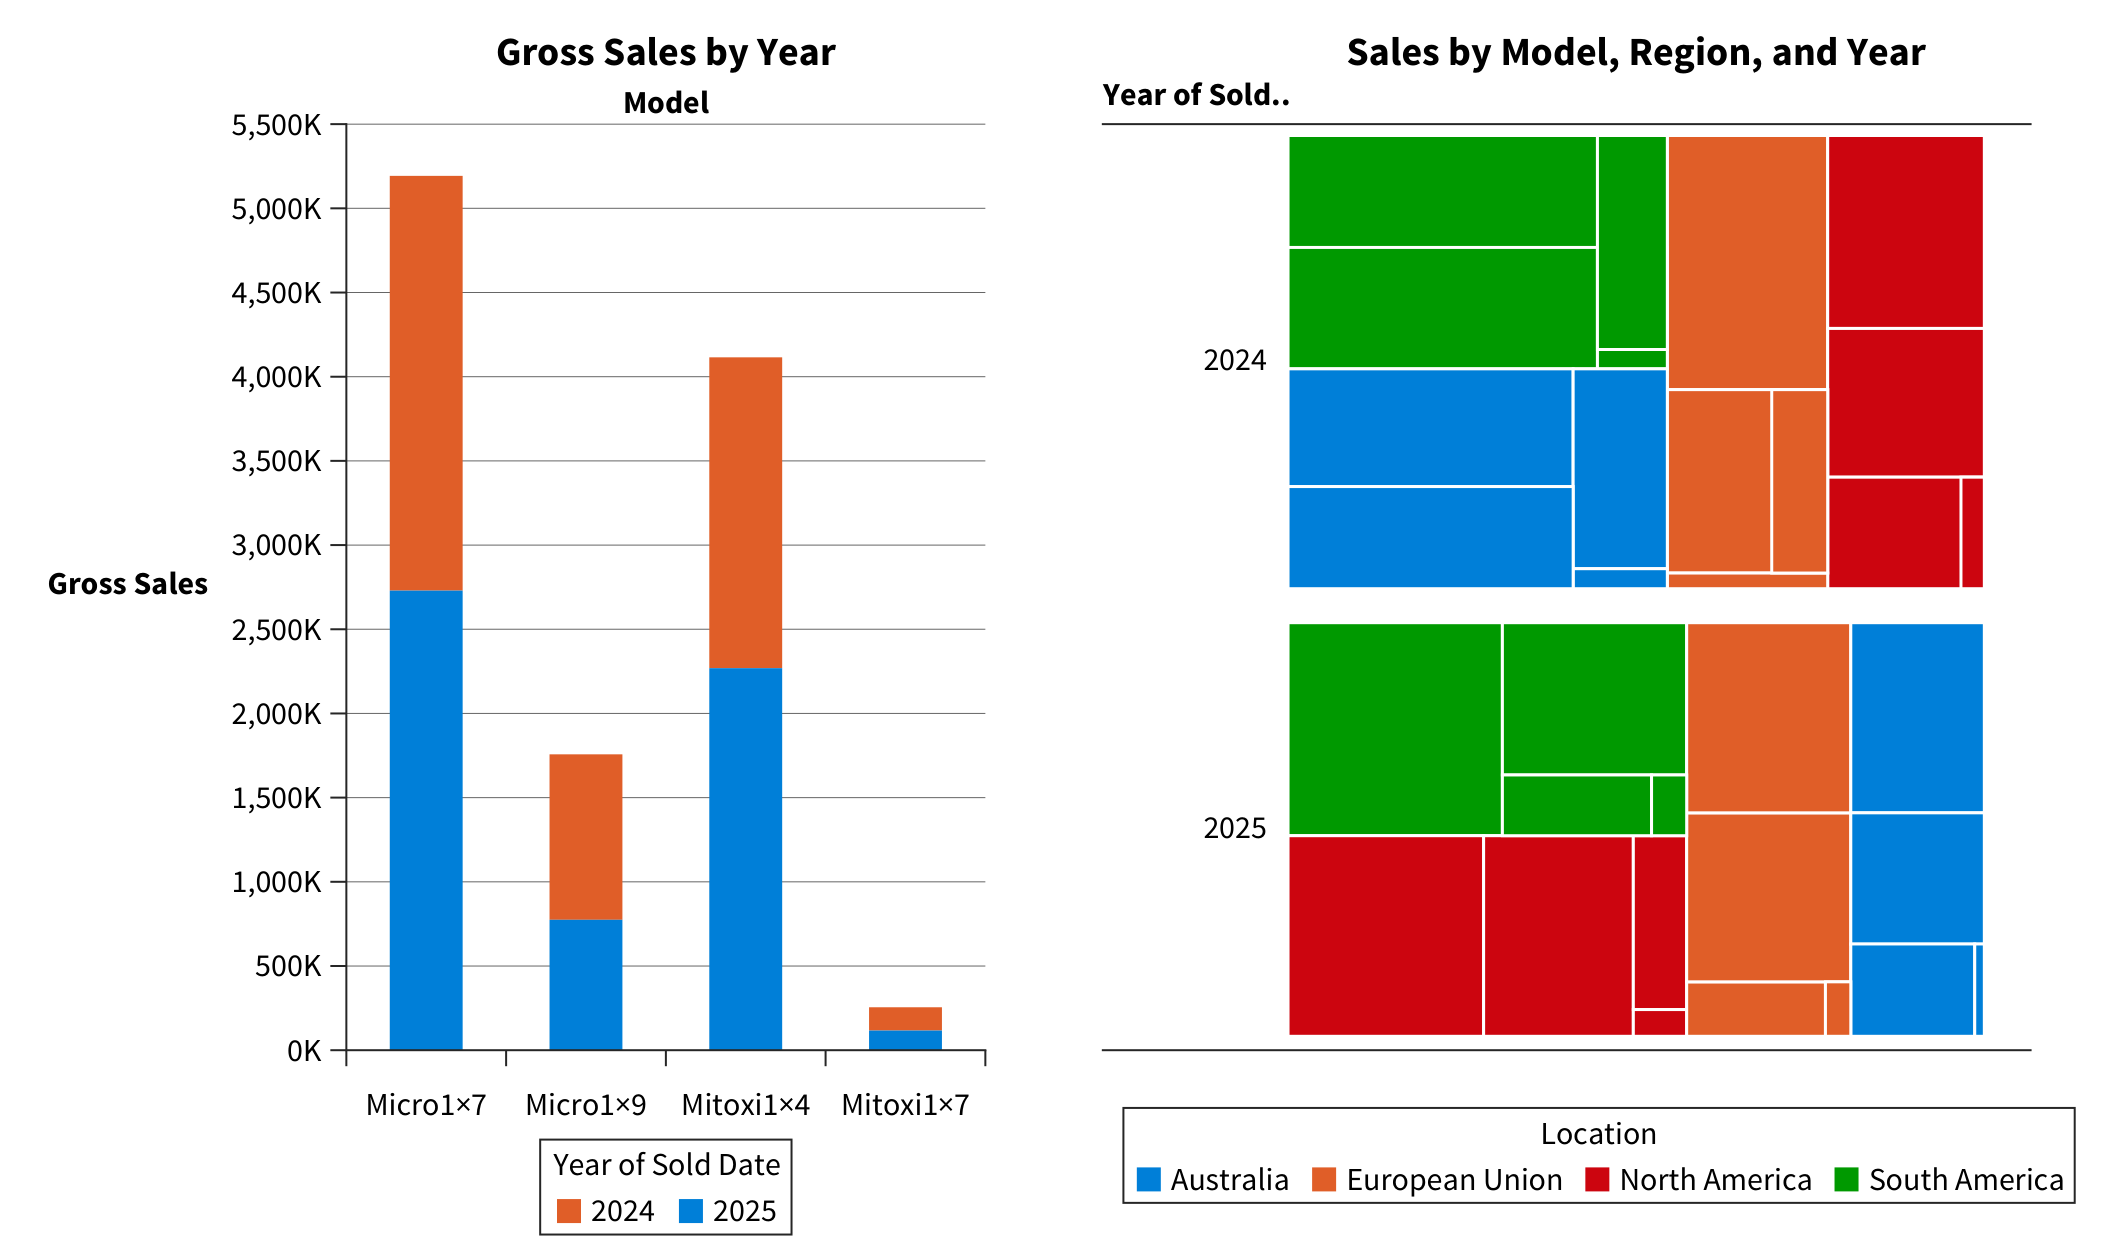
\includegraphics[width=\textwidth,height=0.7\textheight,keepaspectratio]{../textbookForPractice/Figures/Ch_09/EX 9.11.png}
            \end{figure}
        \end{column}
    \end{columns}
\end{frame}

\begin{frame}{EX 9.16 \& EX 9.17}
    \begin{columns}
        \begin{column}{0.5\textwidth}
            \begin{figure}[h]
                \centering
                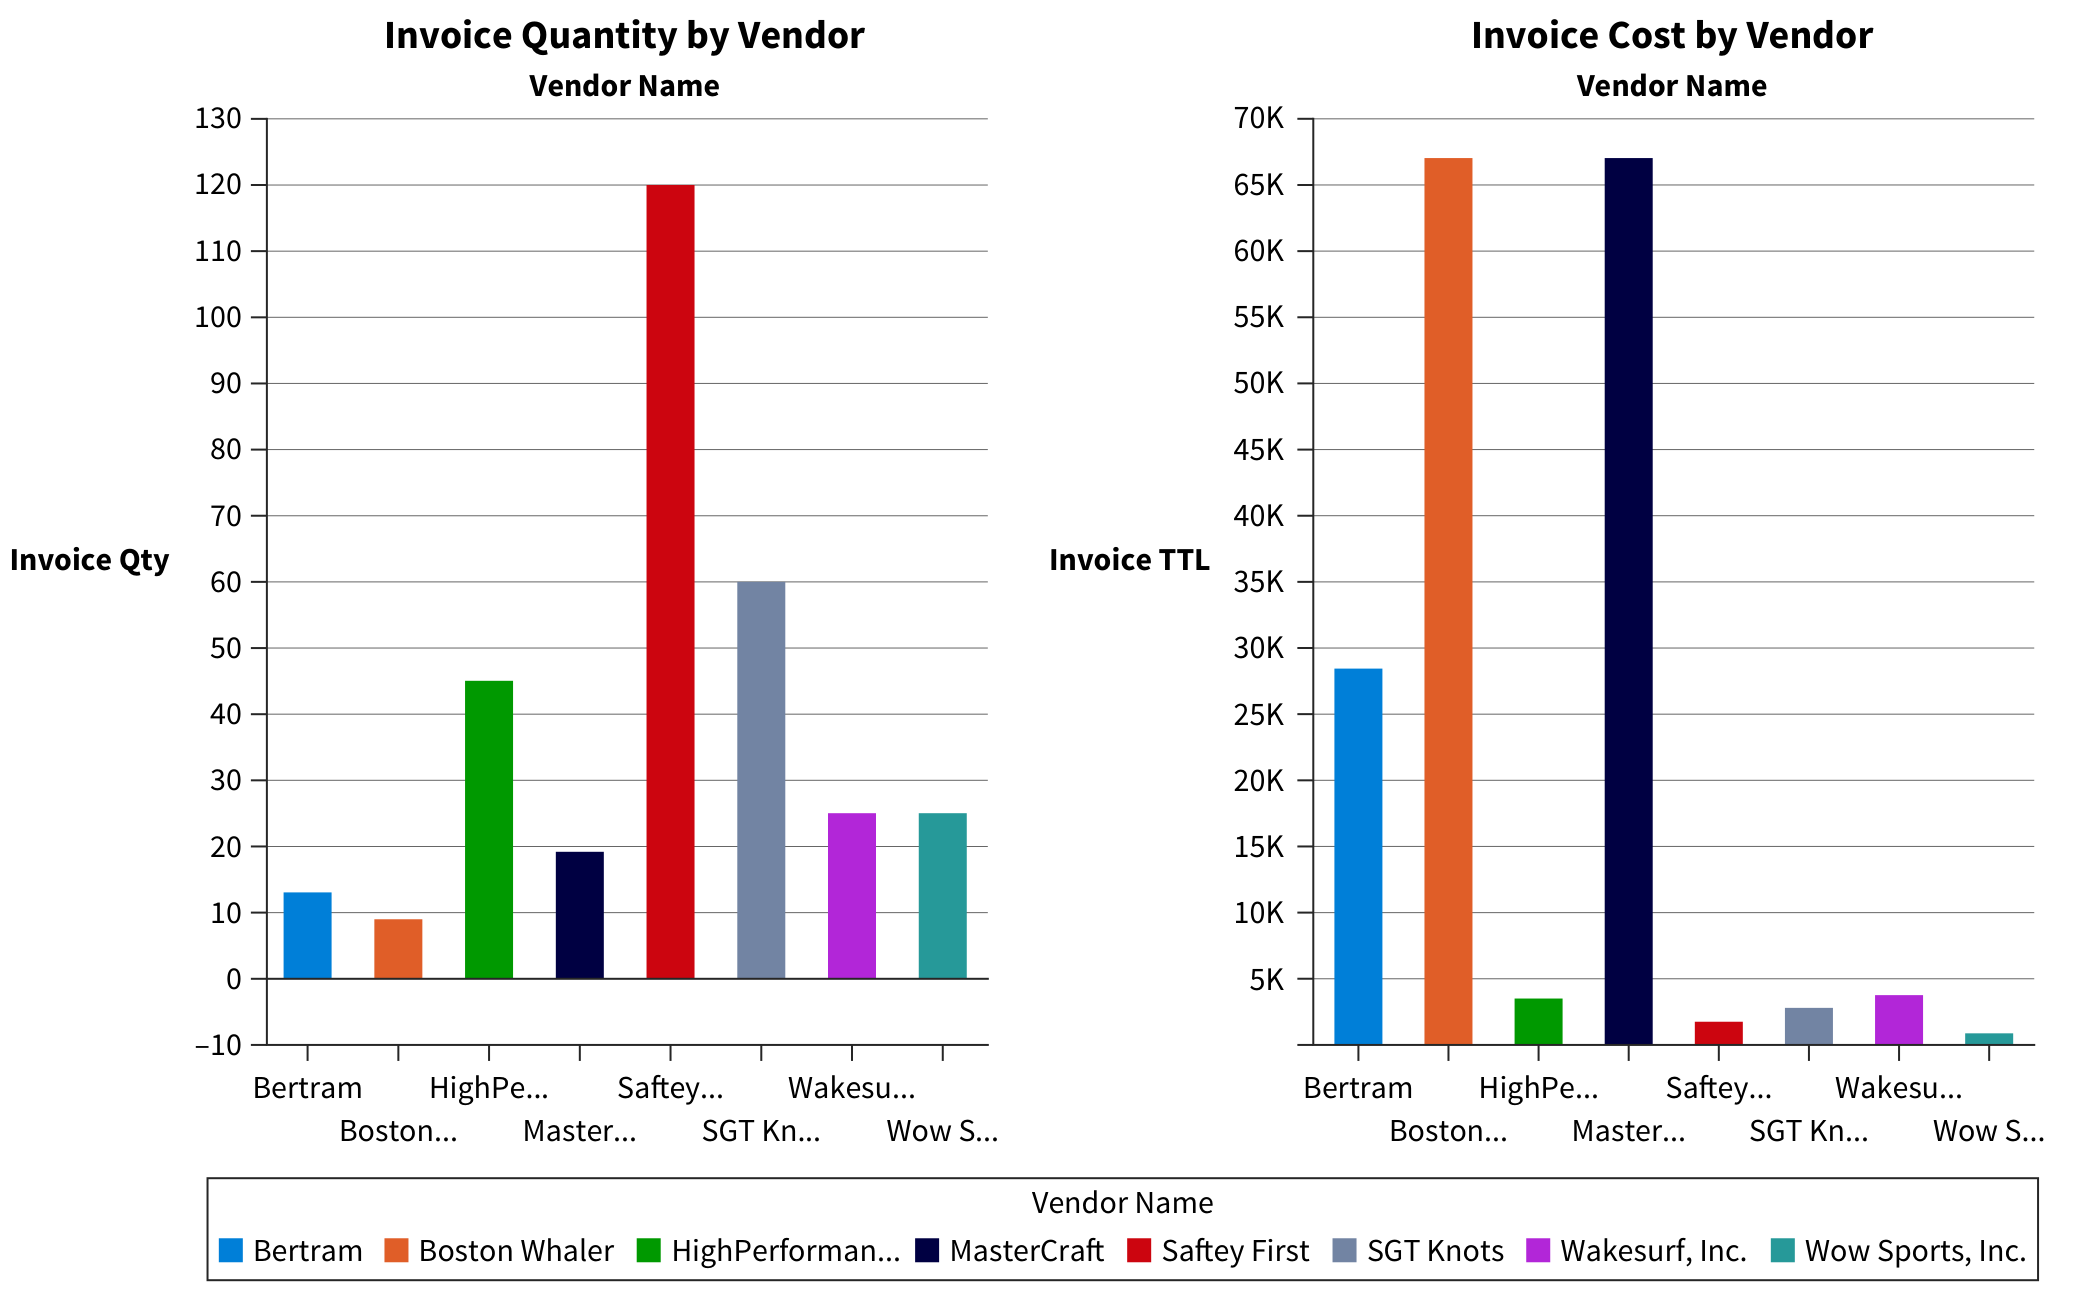
\includegraphics[width=\textwidth,height=0.7\textheight,keepaspectratio]{../textbookForPractice/Figures/Ch_09/EX 9.16.png}
            \end{figure}
        \end{column}
        \begin{column}{0.5\textwidth}
            \begin{figure}[h]
                \centering
                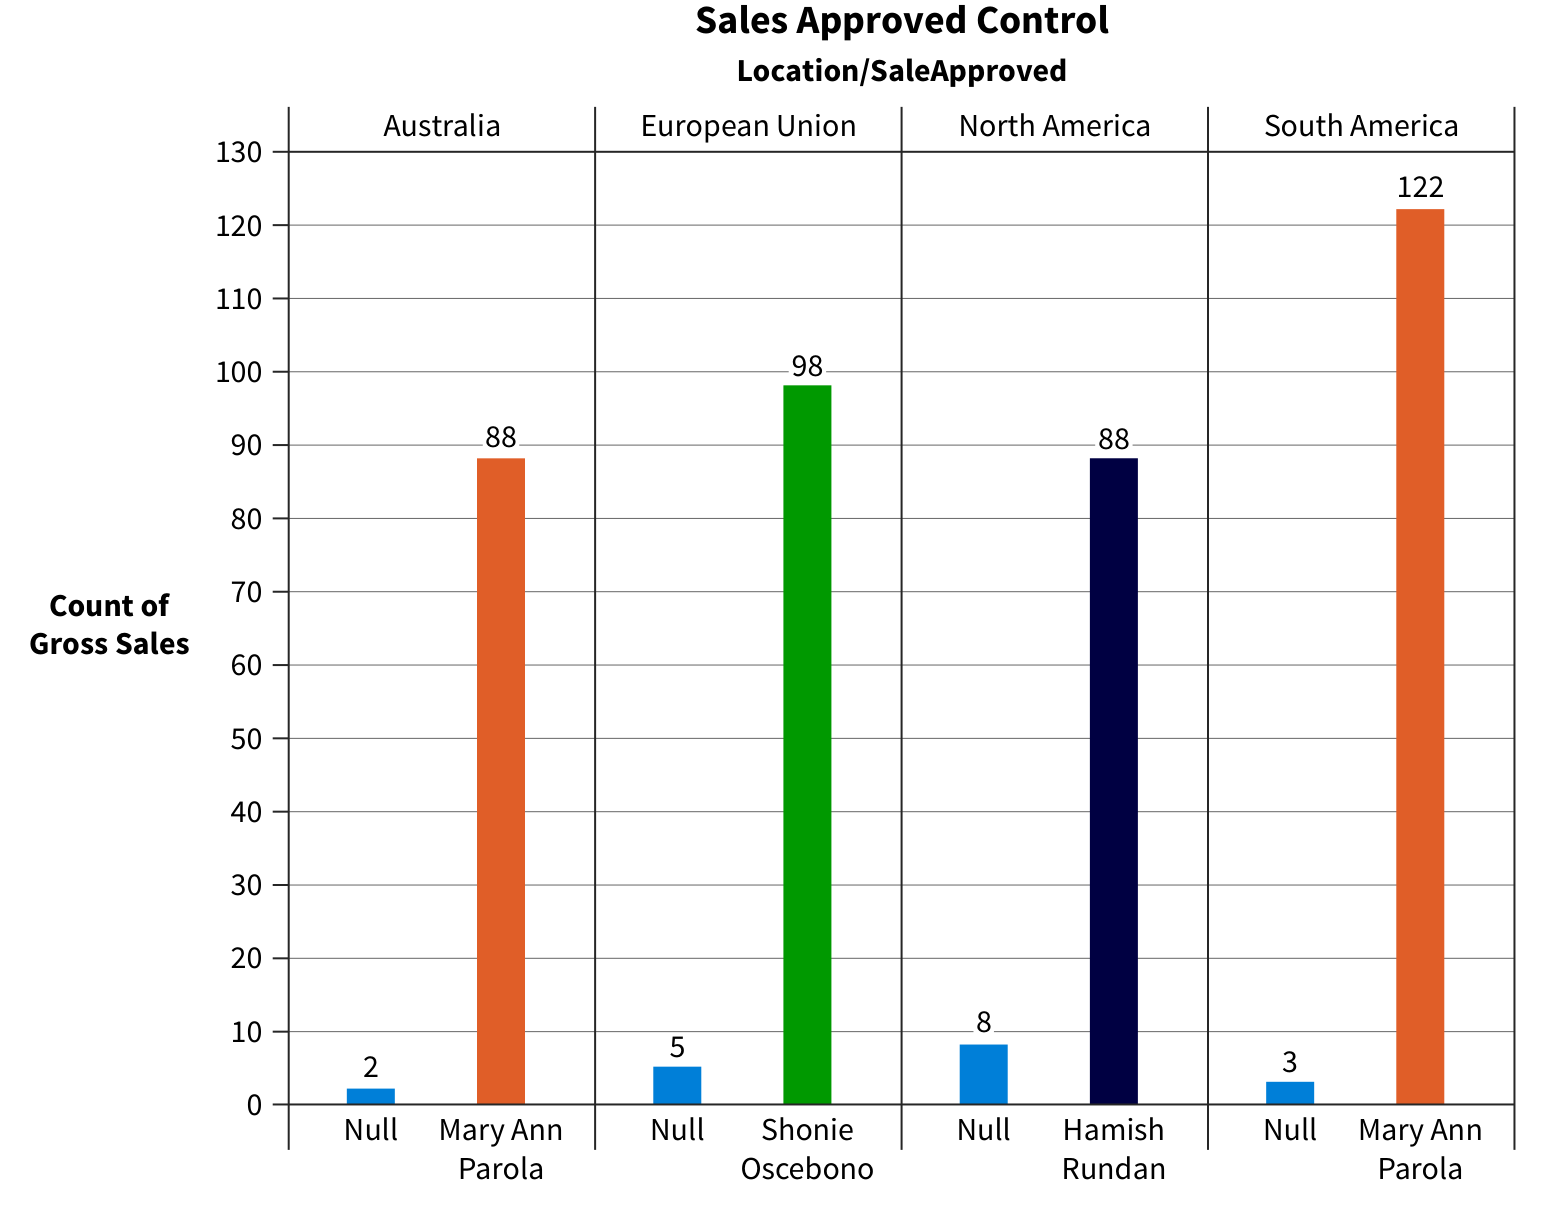
\includegraphics[width=\textwidth,height=0.7\textheight,keepaspectratio]{../textbookForPractice/Figures/Ch_09/EX 9.17.png}
            \end{figure}
        \end{column}
    \end{columns}
\end{frame}

\begin{frame}{EX 9.18 \& EX 9.20A}
    \begin{columns}
        \begin{column}{0.5\textwidth}
            \begin{figure}[h]
                \centering
                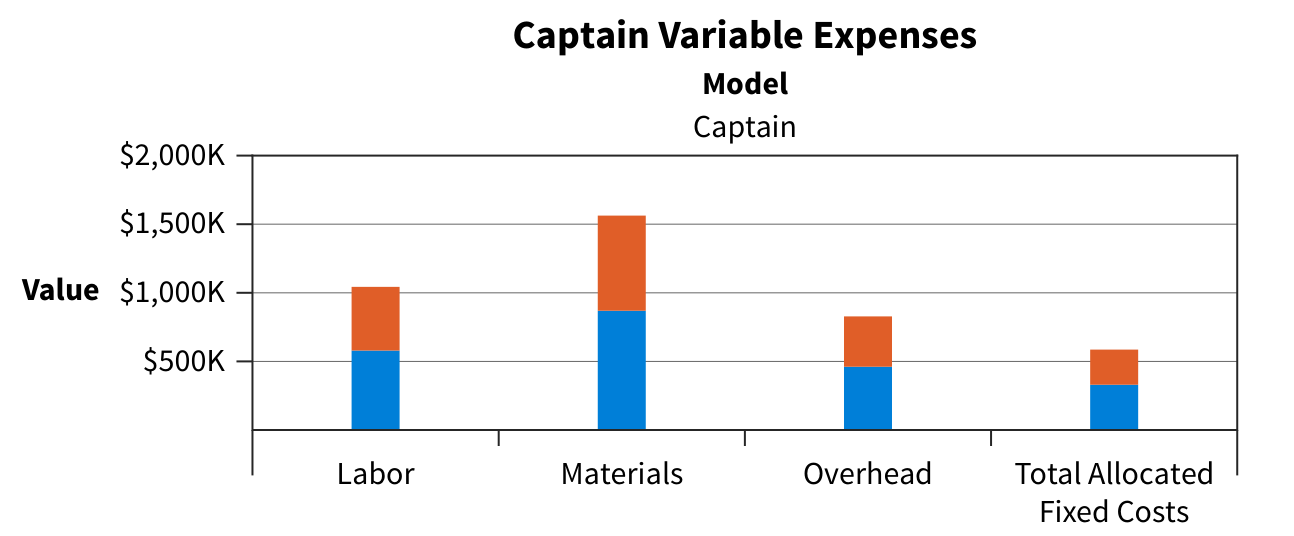
\includegraphics[width=\textwidth,height=0.7\textheight,keepaspectratio]{../textbookForPractice/Figures/Ch_09/EX 9.18.png}
            \end{figure}
        \end{column}
        \begin{column}{0.5\textwidth}
            \begin{figure}[h]
                \centering
                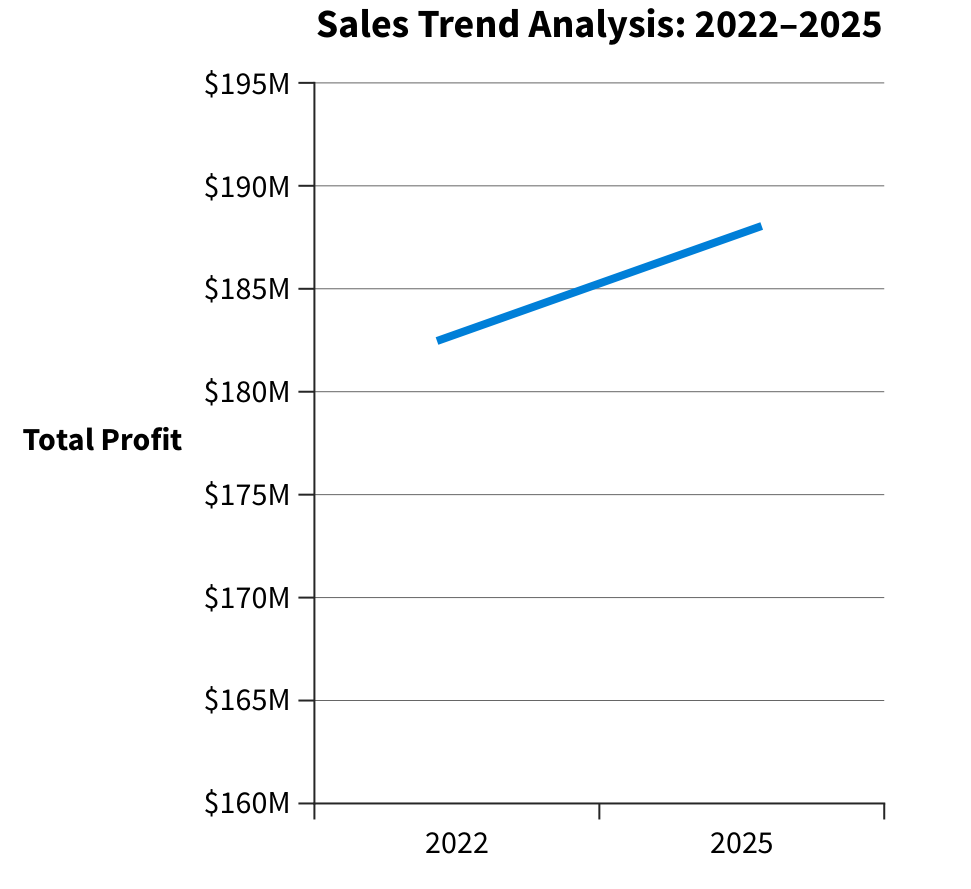
\includegraphics[width=\textwidth,height=0.7\textheight,keepaspectratio]{../textbookForPractice/Figures/Ch_09/EX 9.20A.png}
            \end{figure}
        \end{column}
    \end{columns}
\end{frame}

\begin{frame}{EX 9.20B}

    \begin{figure}[h]
        \centering
        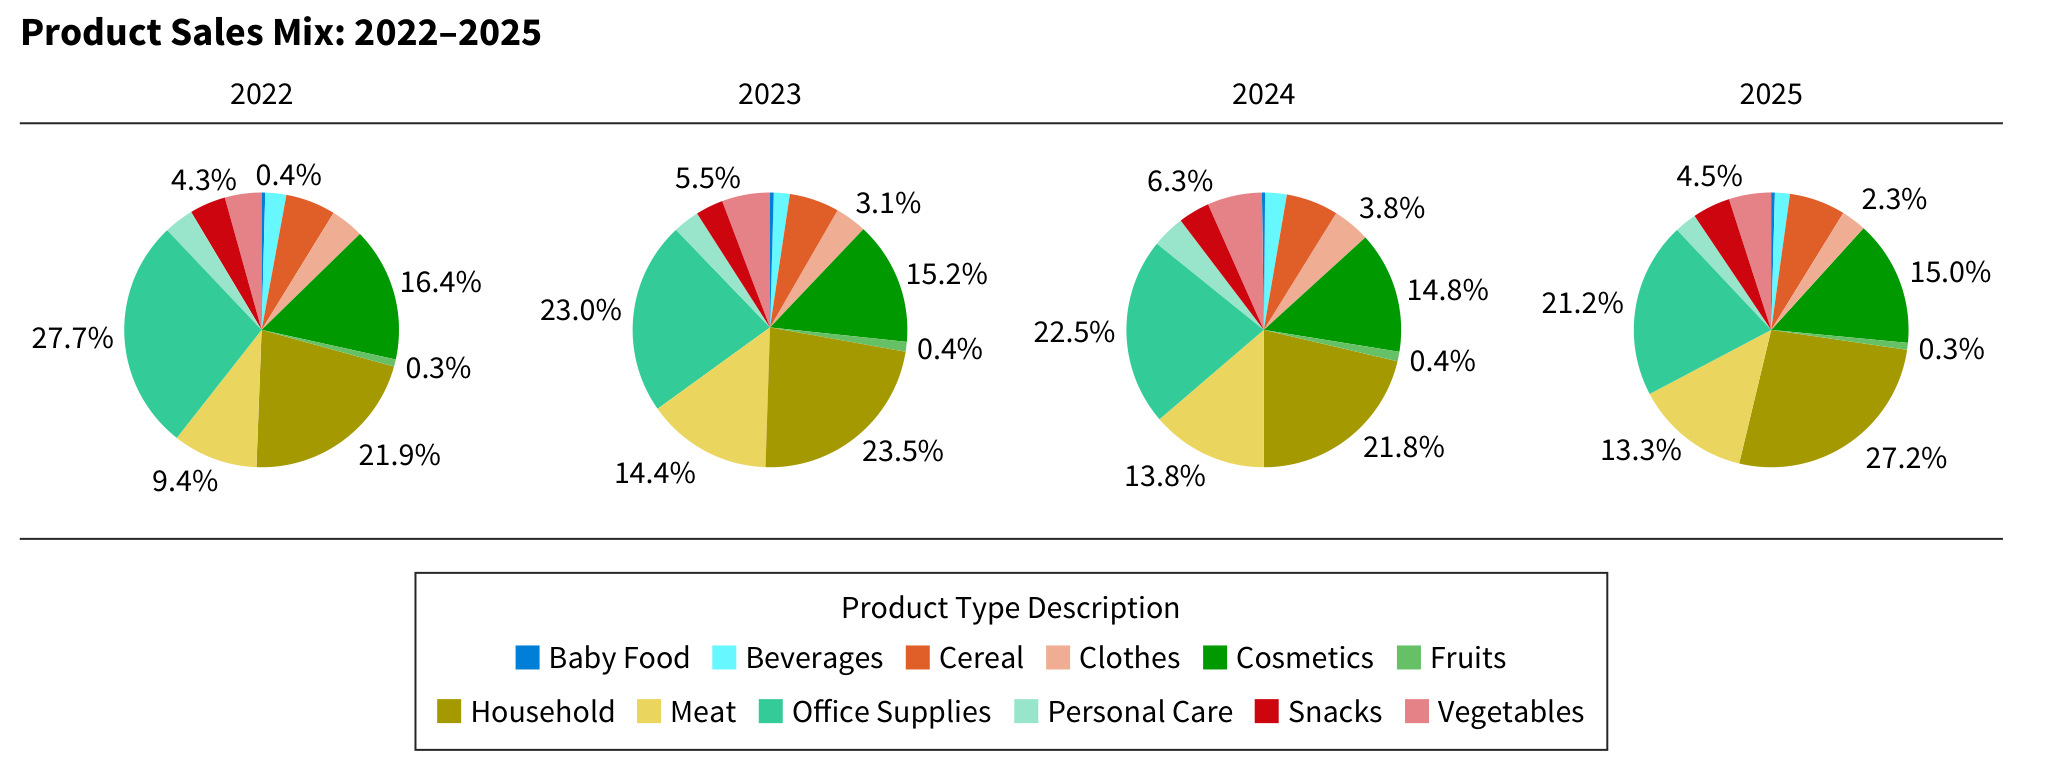
\includegraphics[width=0.95\textwidth,height=0.75\textheight,keepaspectratio]{../textbookForPractice/Figures/Ch_09/EX 9.20B.png}
    \end{figure}
\end{frame}

\begin{frame}{Kết thúc}
    \begin{center}
        \Huge \textbf{Hỏi \& Đáp} \\
        \vspace{1cm}
        \Large Cảm ơn các bạn đã lắng nghe!
    \end{center}
\end{frame}

\end{document}
